%% thesis.tex
%% Walter Dal'Maz Silva
%%
\pdfobjcompresslevel 0
\documentclass[a4paper,french,twoside]{xthesis}

\hypersetup{
    pdftitle    = {Mise au point de la carbonitruration gazeuse des alliages
                  16NiCrMo13 et 23MnCrMo5: modélisation et procédés},
    pdfsubject  = {Traitements thermochimiques},
    pdfauthor   = {Walter Dal'Maz Silva},
    pdfkeywords = {Thermochimie}     {Thermochemistry}
                  {Cinétique}        {Kinetics}
                  {Métallurgie}      {Metallurgy}
                  {Acier}            {Steel}
                  {Carbonitruration} {Carbonitriding}
                  {Cémentation}      {Carburizing}
                  {Austénite}        {Austenite}
                  {Pyrolyse}         {Pyrolysis}
                  {Modélisation}     {Modeling}
                  {Chromatographie}  {Chromatography},
    pdfproducer = {Walter Dal'Maz Silva}
}

%%%%%%%%%%%%%%%%%%%%%%%%%%%%%% New unities and shortcuts

\DeclareSIUnit[]{\atm}{atm}
\DeclareSIUnit[]{\HV}{HV0,3}
\newcommand{\sccm}{\si{\cubic\centi\metre\per\minute}}

%%%%%%%%%%%%%%%%%%%%%%%%%%%%%% Control of print version.

\newtoggle{paper}
\togglefalse{paper}

%%%%%%%%%%%%%%%%%%%%%%%%%%%%%% Document body.

\newcommand{\jury}{
  \footnotesize
  \begin{tabular}{p{0.22\textwidth}p{0.50\textwidth}p{0.28\textwidth}}
  M. M. Gouné
  & Professeur, Université de Bordeaux
  & Rapporteur 
  \tabularnewline[5pt]
  M. C. Vahlas
  & Directeur de recherche, CIRIMAT, Toulouse
  & Rapporteur 
  \tabularnewline[5pt]  
  Mme. M.-L. Giorgi
  & Professeur, LGMP, Châtenay-Malabry
  & Examinateur 
  \tabularnewline[5pt]  
  M. F. Mudry
  & Président, IRT M2P, Metz
  & Examinateur 
  \tabularnewline[5pt]   
  Mme. I. Ziegler-Devin
  & Maître de conférences, LERMAB, Nancy
  & Examinateur 
  \tabularnewline[5pt]  
  M. S. Thibault
  & Docteur-ingénieur, Safran Tech, Magny-les-Hameaux
  & Examinateur 
  \tabularnewline[5pt]
  M. J. Dulcy
  & Ingénieur de recherche, IJL-CP2S, Nancy
  & Examinateur
  \tabularnewline[5pt]  
  M. T. Belmonte
  & Directeur de recherche, IJL-CP2S, Nancy
  & Directeur de thèse 
  \tabularnewline[5pt]
  \end{tabular}
  \par\vskip0.6cm
  Institut Jean Lamour\par
  Département Chimie et Physique des Solides et des Surfaces\par\vfill
  Université de Lorraine \textendash{} Pôle M4 : matière, matériaux, métallurgie, mécanique
}

\logoschool{figures/garde/fig_logoEMMA}
\logocollege{figures/garde/fig_logoUL}
\logopartner{figures/garde/fig_logoIRT}
\logolaboratory{figures/garde/fig_logoIJL}

\jurytable{\jury}
\college{Université de Lorraine}
\school{École Doctorale Énergie Mécanique Matériaux}
\domain{Sciences des Matériaux}
\author{Walter DAL'MAZ SILVA}
\title{Mise au point de la carbonitruration gazeuse des alliages\\ 16NiCrMo13 et 23MnCrMo5: modélisation et procédés}

\begin{document}
  \newpage\setcounter{page}{1}\pagenumbering{roman}
  \cleardoublepage\thispagestyle{empty}\vspace*{\fill}%
\begin{flushright}\begin{minipage}{0.7\textwidth}%
		\begin{flushright}\itshape%
			„Glaube“ heißt Nicht-wissen-wollen, was wahr ist.\par
			(La foi, c'est refuser de connaître la vérité.)
			\par{Friedrich Nietzsche}
		\end{flushright}
\end{minipage}\end{flushright}%
\vspace*{\fill}\clearpage\thispagestyle{empty}\vfill\cleardoublepage
	
\chapter*{Remerciements}

\def\skipaknow{12pt}
\begin{flushright}
\vfill{}

Tout d'abord à mes parents, Deise et Walter, pour avoir proportionné ma vie.\\[\skipaknow]
	
À mes directeurs M. Jacky Dulcy et M. Thierry Belmonte pour leur confiance de m'avoir accepté pour réaliser cette thèse et pour tout leur soutient pendant le développement de ces travaux de thèse.\\[\skipaknow]

À l'IRT M2P pour le financement du projet à travers des partenaires industriels Safran, PSA, Peugeot Citroën, Faurecia, ECM Technologies, Ascometal, Air Liquide, Airbus Helicopters, Arcelor Mittal, UTC Aerospace Systems et Poclain Hydraulics.\\[\skipaknow]

À M. Pascal Lamesle, M. Grégory Michel et M. Simon Thibault pour leur support au cours de mes études. À Mme. Andrea Puech pour tout l'aide avec les aspects administratifs et spécialement pour sa patience avec ma \emph{distance} des aspects bureaucratiques.\\[\skipaknow]

À toute l'équipe de l'IJL, spécialement à M. Francis Kosior, pour son aide dans le monde du numérique. À M. Jaafar Ghanbaja et son inséparable microscope pour les plus belles micrographies en transmission et pour tout le partage de ses connaissances.\\[\skipaknow]

À M. Abdelkrim Redjaïmia pour nous avoir clarifié les résultats obtenus en diffraction d'électrons. À Mme. Christine Gendarme pour la réalisation des analyses chimiques des profils de diffusion et pour sa patience avec mon incapacité de polir l'emboutissage métallique.\\[\skipaknow]

À \emph{Baloo048} pour avoir proportionné des moments de simulation et programmation indescriptibles. Pour toutes les nuits que passées ensemble.\\[\skipaknow]

À mes amis Edgar Castro et Antonio Olmedilla pour être toujours disponibles pour discuter et boire un verre avec moi. À Bruno Borges Ramos pour son retard éternel à venir.\\[\skipaknow]

%À Isadora Deschamps pour m'avoir motivé de quitter ma zone de confort pour démarrer cette thèse. Pour toutes les années que je ne vais jamais oublier.\\[\skipaknow]

À Nancy Perdomo pour son amour.
\vfill{}
\end{flushright}

\cleardoublepage\phantomsection
\pdfbookmark{Resume}{Resume}
\chapter*{Résumé}

Le développement de matériaux d'ingénierie combinant ténacité et résistance à l'usure reste encore un défi. Dans le but de contribuer à ce domaine, cette thèse présente une étude de la carbonitruration des aciers 16NiCrMo13 et 23MnCrMo5. L'évolution cinétique des atmosphères à base d'hydrocarbures et d'ammoniac est étudiée numériquement, ainsi que le comportement local à l'équilibre et la cinétique de diffusion pour l'obtention de profils d'enrichissement des alliages traités. Les simulations sont confrontées à des mesures par chromatographie en phase gazeuse des produits de pyrolyse de l'acétylène et de décomposition de l'ammoniac, et aux réponses métallurgiques, par l'évaluation des profils de diffusion, des filiations de dureté et par l'identification des précipités formés par microscopie électronique en transmission. La dureté obtenue après trempe et traitement cryogénique évolue selon la racine carrée de la teneur en interstitiels en solution solide simulée à partir de la composition locale en utilisant des mesures des profils chimiques en carbone et en azote. Après revenu, les zones enrichies en azote montrent une tenue en dureté supérieure à celles obtenues avec la même teneur totale en carbone en solution, ce qui a été attribué après observation par microscopie électronique en transmission à une fine précipitation de nitrures de fer lors de cette dernière étape de traitement. Le bilan de matière des produits de pyrolyse montre que les principales espèces non détectées sont des radicaux fortement carbonés qui peuvent aussi donner lieu à la formation d'hydrocarbures polycycliques de haut poids moléculaire dans les zones froides du réacteur. À la pression atmosphérique et à basse pression l'établissement de conditions d'enrichissement en carbone à concentration constante est possible en utilisant de faibles pressions partielles d'acétylène dilué dans l'azote. La conversion atteinte par la pyrolyse de ce précurseur est pourtant importante à la température de traitement compte tenu du temps de séjour caractéristique du réacteur employé à la pression atmosphérique. La cinétique de décomposition de l'ammoniac étant beaucoup plus lente que celle des hydrocarbures légers, il a été possible de quantifier la vitesse de décomposition de cette espèce par unité de surface métallique exposée pendant la durée d'un traitement.

\par\vskip0.6cm
\noindent\textbf{Mots-clés:} Carbonitruration; Traitements thermochimiques; Martensite; Cinétique chimique; Modèles de réacteur.

\clearpage\phantomsection
\pdfbookmark{Abstract}{Abstract}
\chapter*{Abstract}

The development of engineering materials combining both toughness and wear resistance is still a challenge. Aiming to contribute to this field of study, this thesis presents a study of the carbonitriding process of alloys 16NiCrMo13~and 23MnCrMo5. Kinetics of hydrocarbon- and ammonia-based atmospheres, as well as local equilibrium and diffusion kinetics for achieving the enrichment profiles, are studied by numerical simulation. These simulations are compared to chromatography measurements of gas phase pyrolysis products of acetylene and ammonia decomposition, and with metallurgical responses, where the comparison is made with evaluated diffusion profiles, hardness measurements and the identification of precipitates by transmission electron microscopy. Hardness after quench and cryogenic treatment depends on the square root of total solid solution interstitial content simulated by using local carbon and nitrogen compositions obtained experimentally. After tempering, the regions enriched in nitrogen show better hardness stability than those with same total carbon interstitial content, what was linked to a fine precipitation of iron nitrides observed by transmission electron microscopy. Mole balance of pyrolysis products show that the main non-detected species are high-carbon radicals, which may also lead to the formation of polycyclic aromatic hydrocarbons of high molecular weight at the reactor outlet. At both atmospheric and reduced pressures, constant concentration enrichment boundary conditions were established by using low partial pressures of acetylene diluted in nitrogen. Pyrolysis of this precursor attains high conversion rates at treatment conditions given the important residence time of the atmospheric pressure reactor. Ammonia decomposition kinetics being much slower than that of low molecular weight hydrocarbons, it was possible to identify the decomposition rate of this species over a metallic sample during  a treatment. 

\par\vskip0.6cm
\noindent\textbf{Keywords:} Carbonitriding; Thermochemical treatments; Martensite; Chemical kinetics; Reactor models.

\endinput

  \cleardoublepage
  \tableofcontents
  \newpage\setcounter{page}{1}\pagenumbering{arabic}
  \part*{Introduction générale}
  \cleardoublepage\chapter*{Introduction générale}

Le développement de matériaux d'ingénierie qui combinent ténacité et résistance à l'usure et à la fatigue reste aujourd'hui encore un défi. Parmi les facteurs qui limitent la production de ce type de matériaux, on peut citer l'incompatibilité intrinsèque qui existe entre ténacité et dureté. Les facteurs économiques limitant la production de matières premières avec un niveau d'inclusions très réduit, la difficulté de maîtriser les procédés existant au niveau industriel, entre autres, imposent des contraintes à ce type de développement.

Cette thèse a pour but de contribuer à la compréhension des phénomènes régissant la carbonitruration d'aciers faiblement alliés à partir d'hydrocarbures et d'ammoniac, en particulier les alliages 16NiCrMo13 et 23MnCrMo5, et leurs réponses métallurgiques. Le procédé de carbonitruration est l'objet central de la présente étude qui traite en particulier du couplage entre cinétique chimique, hydrodynamique et transformations métallurgiques en phase solide. L'approche utilisée vise à améliorer la maîtrise à l'échelle industrielle de ce traitement basé plus spécifiquement sur l'utilisation à basse pression d'acétylène comme source première de carbone. Cela intègre des aspects à la fois expérimentaux mais aussi de modélisation, permettant à terme d'assurer le transfert des résultats de l'échelle laboratoire à l'industrie. De manière plus spécifique, les études réalisées visent à:
\begin{itemize}
  \item comprendre le rôle de l'azote sur les réponses mécaniques et métallurgiques des alliages 16NiCrMo13 et 23MnCrMo5. Cela peut être divisé en
  \begin{inparaenum}[(i)]
    \item l'étude de l'influence de l'azote sur la dureté après trempe, c'est-à-dire l'évaluation de l'effet de cet élément en solution dans la martensite et sur la formation d'austénite résiduelle, et
    \item le rôle de cet élément sur le revenu des alliages choisis entre \SIlist{483;673}{\kelvin}, ce qui est évalué par la chute en dureté observée lors des traitements effectués;
  \end{inparaenum}
  \item étudier le comportement cinétique des atmosphères à base de \ch{C2H2} et de \ch{NH3} dans des conditions d'intérêt pour les procédés thermochimiques. Cela se fait à partir des expériences et par modélisation des atmosphères à l'échelle des installations expérimentales utilisées.
\end{itemize}

Les traitements thermochimiques des matériaux métalliques sont réalisés dans des milieux réactifs grâce à une activation le plus souvent thermique et à l'apport des gaz réactifs permettant la modification partielle de la composition chimique du matériau en surface. Ils peuvent également être réalisés par immersion dans des sels fondus, ou être assistés par des décharges électriques~\cite{Chiaverini1988,Steel2006}. Ce mémoire est dédié uniquement aux traitements thermochimiques activés par voie thermique, pour lesquels la modification partielle de la composition de surface est assurée par transfert de matière entre le gaz et le métal. Ce n'est possible qu'en fixant une différence de potentiel chimique entre les constituants de l'atmosphère et ceux du matériau traité~\cite{Slycke1981i,Steel2006}. Ces traitements sont largement employés dans l'industrie pour modifier les propriétés de surface des matériaux métalliques, notamment des aciers. La nitruration, la cémentation, la nitrocarburation, la carbonitruration, la boruration, entre autres, permettent d'assurer des enrichissements de surface en azote, carbone, bore, etc. La Figure~\ref{fig:exemples-pieces} présente des pièces de transmission de puissance typiquement soumises à cette famille de traitements. 

\begin{figure}[!hb]
  \centering
  \resizebox{0.6\textwidth}{!}{
    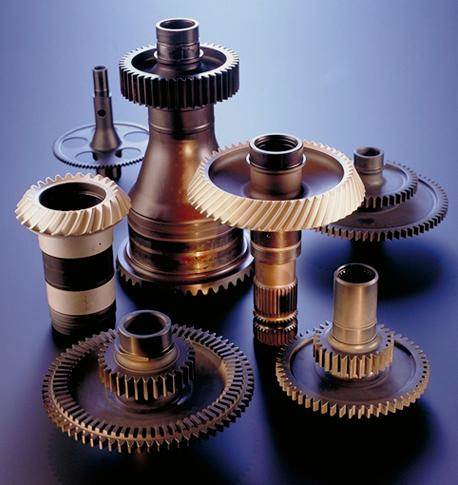
\includegraphics{figures/ch-00-example-pignon}}
  
  \caption{\label{fig:exemples-pieces}Exemples de pièces de transmission de puissance soumises à des traitements thermochimiques (source: Safran Group).}
\end{figure}

Le traitement de carbonitruration est un procédé thermochimique de traitement des matériaux qui, par l'introduction de carbone et d'azote à la surface des aciers, améliore les résistances à la fatigue et à l'usure des pièces traitées. Typiquement, la thermochimie du procédé peut être considérée comme la combinaison d'une cémentation et d'une nitruration dans le domaine austénitique, généralement dans la plage allant de \SIrange{1073}{1173}{\kelvin}~\cite{Slycke1981i,Slycke1981ii}. Bien que la pratique industrielle consiste le plus souvent en l'enrichissement simultané de l'alliage par les deux éléments interstitiels, les résultats présentés ici sont relatifs à un traitement de carbonitruration réalisé comme une séquence d'étapes de cémentation et de nitruration. Cette approche vise à explorer les réponses métallurgiques et mécaniques des alliages étudiés plutôt que les paramètres du procédé de carbonitruration~\cite{Slycke1981i,Sproge1988} et minimise la formation de composants toxiques comme les cyanures pendant le traitement. L'étude de la cinétique gazeuse du procédé se fait d'abord séparément et ses fondements seront abordées à la fin de ce chapitre.

Le plus souvent, le traitement de carbonitruration est effectué sur du fer pur, des aciers faiblement alliés à faible teneur en carbone et des pièces issues de la métallurgie des poudres. Le présent travail traite uniquement du comportement des aciers faiblement alliés. La faible teneur en carbone a pour rôle d'augmenter la cinétique du procédé \textendash{} augmentation du gradient de potentiel chimique entre la surface et le c{\oe}ur du matériau \textendash{} tout en maintenant la ténacité au c{\oe}ur des pièces. Les éléments d'alliage sont destinés à optimiser la trempabilité en surface, promouvoir le durcissement par solution solide à c{\oe}ur et favoriser la précipitation des carbures et nitrures lors du revenu. Comme les fractions d'interstitiels typiquement introduites en surface par le traitement thermochimique sont dans la gamme de fractions massiques allant de 0,005 à 0,007 (en considérant le carbone et/ou l'azote), typiquement une microstructure de martensite en lattes est obtenue dans le gradient de composition~\cite{Steel2006}. La présence d'éléments d'alliage, comme le chrome et le manganèse, implique un comportement différent de celui observé dans le système \ch{Fe-C-N}~\cite{vanGent1985,Mittemeijer1988} en raison de leurs effets sur la transformation martensitique, la résistance au revenu et la précipitation des nitrures à la température de traitement~\cite{Kaplow1983}, ce qui réduit de façon drastique la solubilité de l'azote dans l'austénite.

Le procédé exploite principalement la transformation martensitique pour obtenir les propriétés désirées dans les pièces traitées. Le traitement doit toujours être suivi d'une trempe afin de produire les résultats souhaités. Les contraintes introduites par la trempe dépassent~\footnote{Sur une profondeur qui dépend de la composition de la nuance, de la fraction en interstitiels et des conditions de transfert thermique du milieu de trempe.} l'énergie de déformation requise par la transformation martensitique~\cite{Khachaturyan1983}, ce qui conduit à une phase fragile avec des contraintes internes élevées.  Une dernière étape de revenu \textendash{} typiquement à une température de l'ordre de \SI{473}{\kelvin} \textendash{} est nécessaire pour augmenter la ténacité de la martensite pour les applications visées. Bien que le modèle de \citet{Norstrom1976}, qui sera utilisé dans l'analyse des réponses mécaniques, traduise assez bien le comportement en dureté de la martensite après trempe, les propriétés mécaniques des pièces traitées et revenues dépendent d'une série de mécanismes complexes qui seront abordés tout au long du texte. En outre, la nature des phases à l'équilibre à la température de revenu et leur cinétique de formation jouent un rôle important sur les propriétés finales des alliages qui peuvent s'établir dans des conditions de para--équilibre~\cite{Ghosh2001}.

À l'échelle du laboratoire, le procédé de carbonitruration a fait l'objet d'études à la fois à la pression atmosphérique et sous vide.  En effet, en raison de la maîtrise acquise à l'Institut Jean Lamour sur les processus interfaciaux se déroulant dans un procédé de thermogravimétrie fonctionnant à pression atmosphérique, il a été décidé de bénéficier de cette expérience pour comprendre le comportement métallurgique des nuances traitées, avant de procéder à un transfert des résultats obtenus dans ces conditions à des réacteurs opérant sous vide.

La caractérisation chimique et microstructurale des aciers traités a permis de mieux comprendre le comportement en diffusion-précipitation du carbone et plus spécialement de l'azote dans les deux alliages étudiés.  Le procédé à pression atmosphérique a également fait l'objet de diagnostics par chromatographie en phase gazeuse et par thermogravimétrie, afin de déterminer l'influence des processus de volume par rapport aux processus de surface lors de la décomposition des précurseurs et de l'enrichissement des nuances en carbone et en azote.

Pour la modélisation de l'enrichissement des alliages étudiés, le logiciel Thermo-Calc~\cite{Andersson2002,Borgenstam2000} a été employé~\footnote{L'édition 2015 de ce logiciel intègre déjà Dictra~\cite{Borgenstam2000} comme un module au lieu d'un programme séparé. Dans le texte, si l'on parle de simulation de diffusion avec Thermo-Calc~\cite{Andersson2002,Borgenstam2000}, cela veut dire l'emploi du module Dictra~\cite{Borgenstam2000}}. Ce logiciel permet de traiter la modélisation de la diffusion des éléments interstitiels et de la précipitation de nitrures et de carbures qui décrit les transformations à l'état solide. Les profils de diffusion ainsi obtenus sont comparés à des simulations en utilisant les interdépendances des diffusivités du carbone et de l'azote qui ont été proposées et validées par \citet{Slycke1981ii}. L'étude du comportement cinétique des atmosphères a été réalisée en utilisant un code développé dans les langages de programmation C++ et Python en utilisant les librairies TChem~\cite{Tchem2011} et Cantera~\cite{Cantera2014} pour le calcul des vitesses de réaction et CVode~\cite{Hindmarsh2005} pour l'intégration du système d'équations ainsi généré. Les librairies Boost~\cite{BoostGraph2001} et NetworkX~\cite{Networkx2016} ont été employées dans l'analyse des graphes chimiques permettant l'implémentation de la méthode de \citet{Lu2006i} pour la simplification des systèmes cinétiques et l'obtention de modèles compatibles avec des simulations couplées de la cinétique de décomposition des précurseurs et de l'hydrodynamique du réacteur.

Ce mémoire de thèse est divisé en trois parties: tout d'abord la Partie~\ref{part:part_1} contient une revue bibliographique et théorique des différentes avancées sur les traitements thermochimiques des aciers faiblement alliés. Ensuite, dans la Partie~\ref{part:part_2} est présentée une étude expérimentale des traitements thermochimiques et de la cinétique de décomposition des précurseurs utilisés. Enfin, la modélisation des procédés est traitée dans la Partie~\ref{part:part_3}. Cette thèse s'inscrit dans le cadre d'un partenariat de recherche entre différentes entités académiques et industrielles, réunies dans l'Institut de Recherche Technologique Matériaux, Métallurgie et Procédés (IRT M2P) autour du projet Traitements Thermochimiques Avancées. Les travaux de recherche ont été réalisés au sein de l'Institut Jean Lamour (IJL) à l'Université de Lorraine.

\endinput
  \part{Introduction et fondements théoriques}
  \label{part:part_1}
  \cleardoublepage\chapter{Aspects procédés des traitements thermochimiques}
\label{ch:aspects_procedes}

\vfill

Ce chapitre vise à introduire le sujet et à présenter un état de l'art des traitements thermochimiques par transfert de carbone et d'azote dans les aciers faiblement alliés. Une attention particulière sera accordée à la carbonitruration, procédé utilisé il y a plusieurs décennies avec la cémentation et d'autres procédés de durcissement de surface pour améliorer le comportement mécanique de pièces d'ingénierie~\cite{Slycke1981i}. Pour cela, la Section~\ref{sec:procedes} décrira les principes sous--jacents au contrôle des procédés thermochimiques permettant l'enrichissement en éléments interstitiels comme le carbone et l'azote. Ensuite, les lois de la diffusion à l'état solide et le logiciel Thermo-Calc~\cite{Andersson2002,Borgenstam2000} qui est utilisé pour la simulation des profils de diffusion--précipitation dans les alliages étudiés seront présentés Section~\ref{sec:diffusion}. Les bases de données du logiciel Thermo-Calc~\cite{Andersson2002,Borgenstam2000} contiennent les informations nécessaires aux simulations, \emph{i.e.} des polynômes pour la représentation des propriétés thermodynamiques et de transport. La Section~\ref{sec:dynamique} présente les fondements théoriques requis pour comprendre le couplage hydrodynamique--cinétique qui a lieu au sein des réacteurs réels employés pour des traitements thermochimiques. Finalement, la Section~\ref{sec:cinetique} contiendra les fondements de cinétique chimique selon la loi d'action de masse, ainsi que la méthode de simplification du mécanisme établi afin d'obtenir un nombre réduit d'espèces pour obtenir un modèle moins exhaustif mais plus rapide pour la simulation des écoulements réactifs ayant lieu dans les procédés. 

\vfill\clearpage

\section{Contrôle des procédés thermochimiques gazeux}
\label{sec:procedes}

L'objectif recherché en réalisant des traitements thermochimiques des matériaux métalliques est de transférer des atomes provenant du milieu extérieur à la surface des pièces à partir de réactions hétérogènes~\cite{Gantois2010} et de modifier, dans le cas de la carbonitruration, ses caractéristiques mécaniques. La maîtrise d'un procédé thermochimique comprend l'étude de la cinétique et de la thermodynamique du milieu permettant l'enrichissement de l'interface avec le matériau traité où ont lieu diffusion et transformations métallurgiques.  Cela revient à devoir traiter~\cite{Dulcy2007} le transport des espèces réactives en phase gazeuse vers la surface de l'acier, ce qui inclut la cinétique chimique, la diffusion dans le gaz et l'hydrodynamique du système, les réactions physicochimiques et chimiques à la surface de l'acier et le transport à l'état solide \textendash{} diffusion-précipitation \textendash{} des atomes incorporés par réaction hétérogène. Cet ensemble de phénomènes doit être pris en compte pour simuler le procédé thermochimique au moyen des équations: 
\begin{itemize}
  \item de bilan matière dans le gaz, à l'interface et dans le solide, 
  \item de conservation de la quantité de mouvement et des espèces, 
  \item de transport de la chaleur et de la diffusion de matière.
\end{itemize}

\begin{figure}[h]
  \centering{}
  \resizebox{0.9\textwidth}{!}{%
    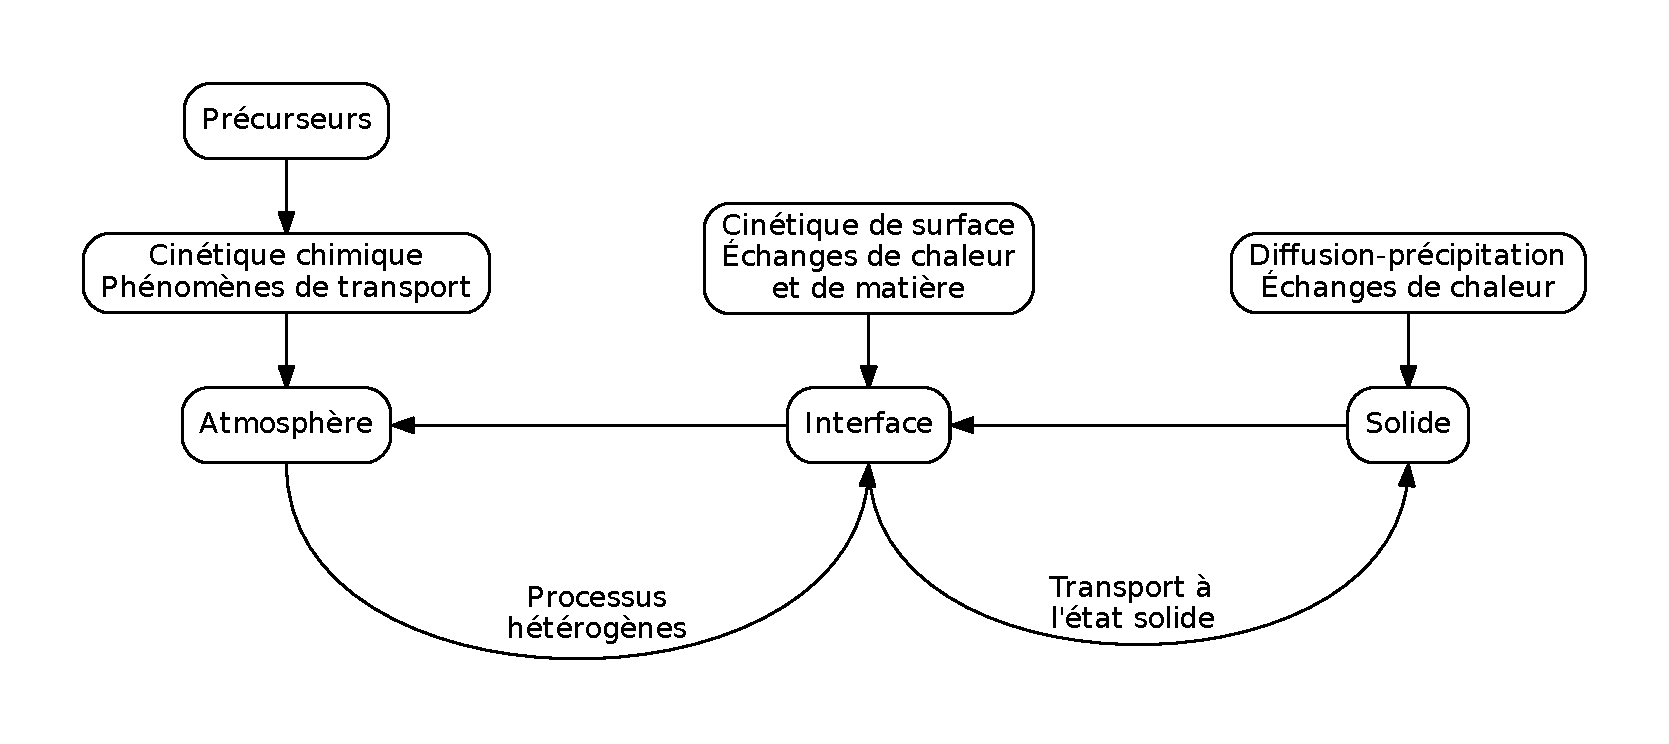
\includegraphics{figures/ch-01-schema-traitements}}
  
  \caption{\label{fig:schema-traitements}Schéma illustrant les principaux processus ayant lieu dans les différentes régions utilisées pour décrire les traitements thermochimiques gazeux.}
\end{figure}

Plusieurs simplifications qui peuvent être mises à profit pour l'optimisation des procédés sont possibles selon le comportement cinétique de l'atmosphère de traitement. Cela peut être illustré, par exemple, dans le cas où l'atmosphère atteint rapidement l'équilibre, cas pour lequel il n'y a pas de couplage entre cinétique et hydrodynamique : l'enrichissement des surfaces peut alors être simplement contrôlé en connaissant l'équilibre gaz--solide. Une autre simplification est possible si l'établissement d'un état stationnaire en phase gazeuse pour un débit donné a lieu. On peut alors considérer un pseudo--équilibre à l'interface gaz--solide. Comme ce travail aborde la carbonitruration comme une série d'étapes successives de cémentation et de nitruration, les discussions sur le contrôle des atmosphères carburantes et nitrurantes se feront séparément. \citet{Slycke1981i} ont abordé l'enrichissement simultané en carbone et en azote.

\subsection{Contrôle de l'étape de cémentation}
\label{sec:controle_cementation}

Le temps caractéristique pour atteindre l'équilibre des atmosphères \ch{CO-H2} dans la plage de température typiquement employée pour la carbonitruration  est court par rapport à la durée de traitement~\cite{Yahia1995,Dulcy2007}. Dans ce cas, l'enrichissement en carbone est indépendant de l'écoulement si le débit total des gaz précurseurs est suffisant pour permettre un enrichissement avec une condition aux limites à concentration constante à l'état stationnaire.  Si ces conditions ne sont pas atteintes, la consommation du carbone disponible dans l'atmosphère est plus rapide que l'arrivée du gaz et une condition à flux variable s'établit. Les paramètres pour établir ce type de contrôle dépendent du volume du four, de la surface totale des pièces traitées, du système de circulation de gaz, etc~\cite{Dulcy2007}. Cette hypothèse d'équilibre permet d'utiliser le potentiel carbone comme paramètre de contrôle du procédé, paramètre dont la définition la plus simple et générale est \og{}\textit{le potentiel carbone d'une atmosphère est la fraction massique en carbone d'un acier en équilibre thermodynamique avec cette atmosphère}~\cite{Dulcy2007}{}\fg.  Cette grandeur, notée $P_{C}$ dans sa représentation en pourcentage massique, est caractéristique de l'atmosphère et n'a de sens que si le système est en équilibre.  À partir des expressions de l'équilibre gaz--solide, on calcule l'activité du carbone dans le matériau. Pour cela, on prend comme état de référence le graphite, comme cela est fait dans l'Équation~\ref{eq:ellis_carbone}~\cite{Dulcy2007}.

\begin{equation}
  a_{C}^{m}=1,07\cdotp Q\cdotp\left(\frac{\si{\%}P_{C}}{100-19,6\si{\%}P_{C}}\right)
    \cdotp\exp\left(\frac{4798,6}{T}\right)
  \label{eq:ellis_carbone}
\end{equation}

Dans cette Équation~\ref{eq:ellis_carbone} le paramètre $Q$ est une fonction de la composition de l'acier et sert à introduire l'influence des éléments d'alliage dans le calcul de l'équilibre entre la fraction massique en carbone dans le matériau et l'activité correspondante dans le gaz. Une des expressions disponibles dans la littérature pour son calcul est fournie par \citet{Gunnarson1967} et est donnée par l'Équation~\ref{eq:gunnarson}.
\begin{equation}
  \begin{split}
  Q=1 & +\si{\%}\ch{Si}\left(0,15+0,033\si{\%}\ch{Si}\right)-0,0365\si{\%}\ch{Mn}
        -\si{\%}\ch{Cr}\left(0,13-0,0055\si{\%}\ch{Cr}\right)\\
      & +\si{\%}\ch{Ni}\left(0,03+0,00365\si{\%}\ch{Ni}\right)
        -\si{\%}\ch{Mo}\left(0,025+0,01\si{\%}\ch{Mo}\right)
  \end{split}
  \label{eq:gunnarson}
\end{equation}

Plusieurs expressions d'équilibre peuvent être écrites pour les atmosphères à base de \ch{CO - H2}. Le choix de l'équilibre considéré pour le réglage du procédé implique la mesure d'une grandeur physique spécifique, ce qui demandera une méthode différente de détection. En général, la mesure de la température du point de rosée, la mesure de la pression partielle d'oxygène ou la mesure par absorption infrarouge de la pression partielle de \ch{CO} sont réalisées dans ce but~\cite{Dulcy2007}. Par exemple, pour un contrôle basé sur la température de point de rosée, l'équilibre en phase gazeuse de la réaction du gaz à l'eau donné par \ch{CO + H2 <=> C_{m} + H2O} et sa constante d'équilibre en termes de pression $K_{p}$ \textendash{} pressions partielles données en \si{\atm} \textendash{} permet d'établir l'expression de l'activité $a_{C}^{g}$ du carbone dans le gaz grâce à l'Équation~\ref{eq:equilibre_point_de_rose}. 

\begin{equation}
  a_{C}^{g}=
  \frac{P\left(\ch{CO}\right)\cdot P\left(\ch{H2}\right)}
  {P\left(\ch{H2O}\right)}\cdot
  \exp\left(\frac{16763}{T}-17,5842\right)
  \label{eq:equilibre_point_de_rose}
\end{equation}

L'hypothèse d'équilibre à l'interface gaz--solide nous permet d'écrire $a_{C}^{m}=a_{C}^{g}$. Cette expression  permet de comprendre les relations entre les paramètres opératoires \textendash{} composition de l'atmosphère et la température \textendash{} et la composition de la nuance traitée \textendash{} en termes du paramètre $Q$ \textendash{} avec la teneur en carbone obtenue en surface \textemdash{} le potentiel carbone $P_{C}$. Pour des alliages différents, la teneur en carbone $P_{C}$ \textendash{} pour une activité constante de l'atmosphère $a_{C}^{g}$ \textendash{} sera d'autant moins importante que la valeur de $Q$ sera élevée. On peut vérifier cela à partir des Équations~\ref{eq:ellis_carbone}~et~\ref{eq:equilibre_point_de_rose} et de la condition d'équilibre $a_{C}^{m}=a_{C}^{g}$ en faisant:

$$
P_{C}=\frac{10000\cdotp{}a_{C}^{m}}{107\cdotp{}Q\cdotp{}{\exp\left(\frac{4798,6}{T}\right)}+1960\cdotp{} a_{C}^{m}}
$$ 

Les Équations~\ref{eq:ellis_carbone}~et~\ref{eq:equilibre_point_de_rose} permettent le calcul de la pression partielle de vapeur d'eau $P\left(\ch{H2O}\right)$ à l'équilibre dans le système. Cette grandeur est utilisée dans l'Équation~\ref{eq:point_rosee} avec la pression de travail $P_{ref}$ du système dans le calcul de la température de point de rosée $T_{r}$ du gaz qui peut être mesurée par des techniques analytiques et permet la mise au point et le suivi du procédé. Cette procédure permet de tracer des diagrammes donnant la température du point de rosée $T_{r}$ en fonction de la fraction massique en carbone pour un alliage spécifique, comme celui de la Figure~\ref{fig:dew_point_iron}.  Les données présentées ont été calculées comme cela est décrit dans cette section et comparées à celles calculées par le logiciel Thermo-Calc~\cite{Andersson2002,Borgenstam2000}, au moyen des bases de données SSUB3 pour l'équilibre en phase gazeuse et TCFE7 pour lier l'activité en carbone à sa fraction massique dans le système \ch{Fe-C}. 

\begin{equation}
T_{r}=\frac{5422,13}{14,7316+\ln\biggr(\dfrac{P_{ref}}{P\left(\ch{H2O}\right)}\biggr)}
\label{eq:point_rosee}
\end{equation}

\begin{figure}[!b]
  \centering
  \resizebox{0.6\textwidth}{!}{
    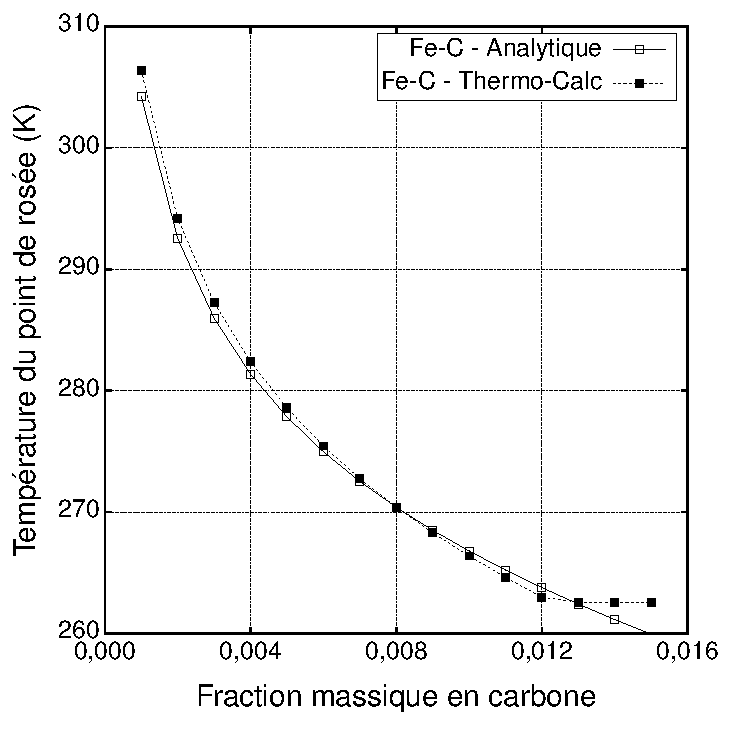
\includegraphics{figures/ch-01-dew_point_iron}}
  
  \caption{\label{fig:dew_point_iron}Température du point de rosée en fonction de la fraction massique en carbone en équilibre avec l'atmosphère pour le système à \SI{1173}{\kelvin}. Atmosphère \ch{N2 - 0,2 H2 - 0,4 CO}.}
\end{figure}

La température de point de rosée requise pour atteindre une fraction massique en carbone visée en surface décroît avec l'augmentation du paramètre $Q$ de l'Équation~\ref{eq:ellis_carbone}. Cela implique donc une pression partielle de l'eau $P\left(\ch{H2O}\right)$ en équilibre avec la surface correspondant à cette teneur en carbone plus faible: plus la fraction en carbone visée en surface est élevée, plus la température du point de rosée associée est faible. La méthode analytique proposée n'est valable que jusqu'à la limite de solubilité en carbone, activité $a_{C}^{m}={1}$. Dans le cas du système binaire \ch{Fe-C}, la fraction massique en carbone dans le matériau devient indépendante de la température du point de rosée $T_{r}$, étant donné qu'il est impossible d'avoir de la diffusion en domaines biphasés dans des systèmes binaires. Cela implique le besoin d'un contrôle précis de $T_{r}$ au voisinage de la limite de solubilité pour limiter la précipitation de cémentite.  Ce n'est pas le cas pour des alliages de fer et des considérations supplémentaires sont alors nécessaires \textemdash{} Section~\ref{sec:classical_carburizing}.

Le contrôle des atmosphères d'hydrocarbures est rapporté par \citet{Yada2013} qui montrent que pour de faibles pressions partielles \textendash{} de l'ordre de \SI{50}{\pascal} \textendash{} il est possible d'atteindre la condition de saturation en surface pour des aciers faiblement alliés. Cependant, les auteurs~\cite{Yada2013} ont réalisé un enrichissement à la saturation en carbone de l'austénite et leurs conditions expérimentales ne sont pas représentatives des réacteurs de grandes dimensions où la décomposition de l'acétylène peut être importante. Cela fait l'objet du Chapitre~\ref{ch:caracterisation_atmospheres} qui traitera des mécanismes de décomposition des hydrocarbures disponibles dans la littérature~\cite{Benzinger1996957,Becker1998177,Becker1998201,Becker1998213, Becker1998225,Norinaga2005,Norinaga2007,Norinaga2007ii,Graf2007,Khan2008, Norinaga2009,Lacroix2010132,Gorockiewicz2011,Fau2013,Ziegler2005107,Ziegler2005212,Ziegler2005231,Ziegler2007268,Ziegler201348} et de leur cinétique, puis du Chapitre~\ref{ch:modelisation_cinetique} pour leur simulation numérique. Autres résultats concernant la cémentation basse pression à partir d'hydrocarbures sont aussi fournis dans la littérature~\citet{Tsuji1987,Liu2003,Iwata2005,Kula2005,Kula201326,Zajusz2014646}.

\subsection{Contrôle de l'étape de nitruration}
\label{sec:controle_nitruration}

La nitruration gazeuse est conduite avec des atmosphères à base d'ammoniac et de ses produits de décomposition~\cite{Slycke1981i,Ginter2006}, comme cela est présenté par la Réaction~\ref{eq:ammonia_hom} et sa constante d'équilibre~\cite{Stolen2004,Landau1980} \textendash{} l'Équation~\ref{eq:ammonia_hom_k} \textendash{} qui vaut $K_{hom}=\SI{1,2E5}{\square\atm}$ à \SI{713}{\kelvin}. Cette valeur montre qu'à cette température, typique pour la nitruration des aciers, l'ammoniac devrait être déjà presque complètement dissocié~\cite{Gantois2010}. Si la température augmente à \SI{1173}{\kelvin}, on obtient $K_{hom}=\SI{2,3E7}{\square\atm}$, valeur qui correspond à une fraction résiduelle en \ch{NH3} de deux ordres de grandeur plus faible que celle disponible typiquement dans la carbonitruration. Selon \citet{Slycke1981i}, cette température impose une limite pratique pour l'enrichissement en azote des aciers faiblement alliés et on ne devrait avoir que du \ch{H2} et du \ch{N2} dans le réacteur. Si l'enrichissement en carbone a lieu en même temps que celui en azote, la fraction résiduelle d'ammoniac ne change pas de façon mesurable~\cite{Slycke1981i}.

\reaction[eq:ammonia_hom]{2 NH3 <=> N2 + 3 H2}

L'Équation~\ref{eq:ammonia_hom_k} devrait permettre de calculer la fraction molaire résiduelle d'ammoniac disponible dans le four pour permettre le transfert de matière vers le solide: ce n'est pas le cas étant donnée la cinétique de décomposition de \ch{NH3}. Selon \citet{Gantois2010} \og\textit{la faible vitesse de dissociation thermique de la molécule de \ch{NH3} en phase gazeuse implique que celle-ci se trouve dans un état de pseudo-équilibre thermodynamique vis-à-vis du temps de séjour relativement court des molécules dans le réacteur, généralement de l'ordre de quelques minutes}\fg{} à la pression atmosphérique. Les temps de séjour dans les traitements thermochimiques à basse pression sont environ de deux ordres de grandeur plus courts. Cela implique que le contrôle du procédé dépend de l'hydrodynamique du réacteur~\cite{Slycke1981i,Ginter2006}, qui impose un temps de séjour moyen des molécules en phase gazeuse dépendant principalement du débit volumique du gaz vecteur~\cite{Gantois2010}.

\begin{equation}
K_{hom}\left(T\right)=
\frac{P\left(\ch{N2}\right)\cdot
  P\left(\ch{H2}\right)^{3}}{P\left(\ch{NH3}\right)^{2}}=
\exp\left[2,3\cdot\biggr(12,392-\frac{5886}{T}\biggr)\right]
\label{eq:ammonia_hom_k}
\end{equation}

Le contrôle du débit des précurseurs permet l'établissement d'une fraction résiduelle constante d'ammoniac dans le gaz. C'est donc cette fraction résiduelle qui doit être en équilibre avec l'azote dans l'acier, comme cela est imposé par la Réaction~\ref{eq:ammonia_het} et sa constante d'équilibre \textendash{} Équation~\ref{eq:ammonia_het_k} \textendash{} \cite{Slycke1981i,Yahia1995}. C'est cette réaction globale avec le solide qui constitue l'étape limitante du procédé dans le cas du fer~\cite{Slycke1981i} et de ses alliages. D'un point de vue élémentaire, l'équilibre précédent est géré par des déshydrogénations successives de l'ammoniac, si bien que l'étape élémentaire limitante dépend des caractéristiques de la surface traitée et bien sûr de la température~\cite{Aparicio1994}.  L'augmentation de la température favorise la formation des produits dans les Réactions~\ref{eq:ammonia_hom}~et~\ref{eq:ammonia_het}, ce qui est mis en évidence par les Équations~\ref{eq:ammonia_hom_k}~et~\ref{eq:ammonia_het_k}, qui présentent des dérivées positives par rapport à la température. Il y a donc une compétition entre l'apport d'azote dans l'austénite et sa décomposition homogène. 

On doit aussi remarquer que l'équilibre introduit des contraintes additionnelles comme la réaction de denitruration \ch{N$^{s}$ <=> 1/2 N2$^(g)$} et peut conduire à la formation de défauts dans la couche: lors de l'interruption de l'apport en \ch{NH3}, le mécanisme de rétro--diffusion d'azote est régi en surface par le processus indirect de la Réaction~\ref{eq:ammonia_het}, ce qui peut provoquer une perte importante de masse. Le procédé peut encore conduire à la formation de gaz \ch{N2} aux joints de grains et autres défauts cristallins où peuvent alors se concentrer ces molécules et promouvoir la formation de porosités. Lorsque des pressions de l'ordre de quelques centaines d'atmosphères s'exercent dans les pores et que les températures sont élevées, la déformation plastique du matériau, associée à la coalescence des pores, conduit à l'apparition de défauts de surface macroscopiques. Les paramètres importants pour la compréhension de la formation de porosité sont donc la température, la durée du traitement et l'activité de l'azote dans l'austénite~\cite{Yahia1995}.  \citet{Yahia1995} observe la formation de porosités dans les échantillons de nuance XC10 avec une fraction massique en azote de 0,006 en surface. Pour les nuances traitées ici, cette teneur doit être plus élevée, dans la mesure où la présence d'éléments d'alliage (principalement le \ch{Cr}) diminue l'activité de l'azote par formation de précipités. Comme cette limite (une fraction massique $w_{N}=0,006$) se situe au-delà de celle définie dans cette étude ($w_{N}=0,004$), la formation importante de porosités n'est pas attendue.
%prévue dans les conditions étudiées.

\reaction[eq:ammonia_het]{NH3 <=>[s] N^s + 3/2 H2}

\begin{equation}
  K_{het}\left(T\right)=
  \frac{a_{N}^{m}\cdot
  P\left(\ch{H2}\right)^{\frac{3}{2}}}{P\left(\ch{NH3}\right)}=
  \exp\left[2,3\cdot\left(6,196-\frac{2943}{T}\right)\right]
  \label{eq:ammonia_het_k}
\end{equation}

C'est à partir de ce pseudo--équilibre que \citet{Lehrer1930} dans les années 1930 a établi pour \ch{Fe-N} un diagramme de phases en fonction d'une grandeur appelée potentiel de nitruration, défini par $K_{N}=\nicefrac{P\left(\ch{NH3}\right)}{P\left(\ch{H2}\right)^{\nicefrac{3}{2}}}= \nicefrac{a_{N}^{m}}{K_{het}}$. Dans cette équation $a_{N}^{m}$, l'activité de l'azote dans l'alliage est une fonction de la teneur en azote $N_{m}$ dans le métal et la relation dépend du modèle de solution adopté. L'équation donnant le $K_{N}$ peut être résolue pour des alliages industriels à l'aide du logiciel Thermo-Calc~\cite{Andersson2002,Borgenstam2000}. Cela permet d'obtenir des diagrammes $K_{N}\text{ vs }N_{m}$ et donc, de déterminer la composition de l'atmosphère permettant d'atteindre la teneur en azote désirée en surface des pièces traitées. La Figure~\ref{fig:diagrammes_kn} présente ces diagrammes pour les alliages étudiés en considérant plusieurs teneurs en carbone et utilisant le diazote à la pression atmosphérique comme état de référence de l'azote \textemdash{} voir Annexe~\ref{an:nitriding-kn}. Il faut prendre en compte le fait que c'est la teneur résiduelle de \ch{NH3} dans l'atmosphère qui permet ce calcul de pseudo--équilibre. D'autres expressions pour décrire l'équilibre gaz--matériau
%, en plus des développements de \citet{Lehrer1930}, 
sont réunies dans une synthèse écrite par \citet{Gantois2010}.

\begin{figure}[!ht]
  \centering
  \subfloat[16NiCrMo13]{
    \centering\resizebox{0.48\textwidth}{!}{
      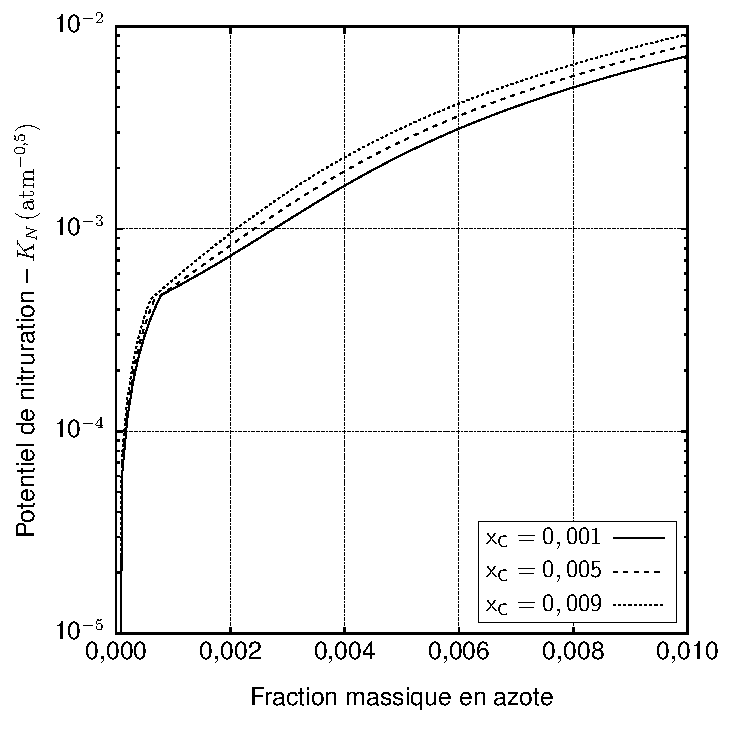
\includegraphics{figures/ch-01-kn_diagram_aero}}
  } \hfill 
  \subfloat[23MnCrMo5]{
    \centering\resizebox{0.48\textwidth}{!}{
      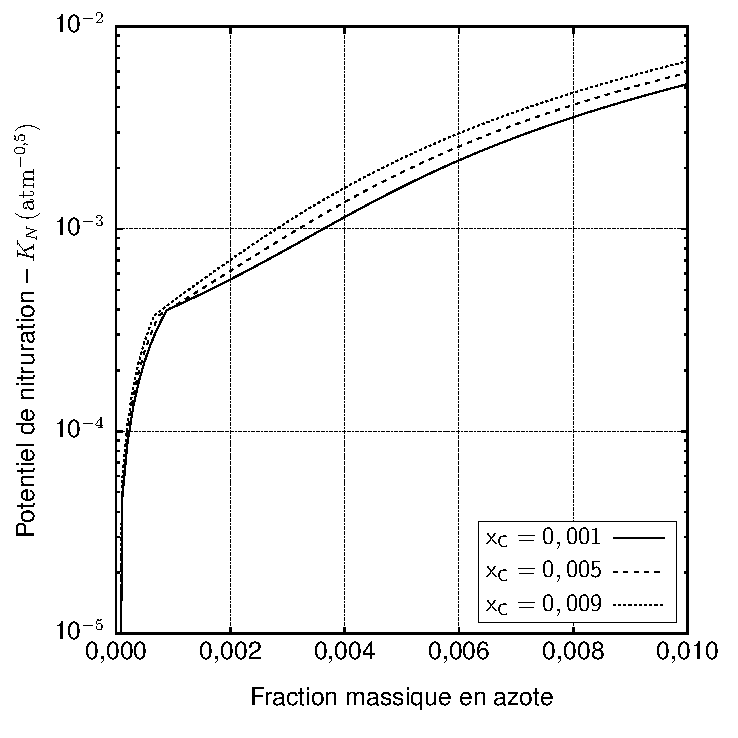
\includegraphics{figures/ch-01-kn_diagram_auto}}
  }

  \caption{\label{fig:diagrammes_kn}Diagrammes donnant le potentiel de nitruration en fonction de la fraction massique en azote en surface dans les alliages 16NiCrMo13 et 23MnCrMo5.}
\end{figure}

\section{Transport de matière à l'état solide}
\label{sec:diffusion}

\subsection{Fondements théoriques}

Le transport de matière à l'état solide est à la base de la majorité des traitements thermochimiques. L'introduction des éléments carbone et azote lors de la carbonitruration se fait à partir d'une réaction de surface entre la pièce et le milieu servant au traitement et ensuite par diffusion de ces éléments vers le c{\oe}ur des pièces traitées~\cite{Slycke1981i}.  Cette migration des atomes se produit par sauts successifs entre les défauts ou espaces vides du cristal sous l'effet de l'agitation thermique.  Si l'on traite la migration des atomes par une méthode statistique, il faut introduire les notions de probabilité de saut, de distance de saut, de directions possibles et de fréquence de vibration atomique~\cite{Jaoul2004}.  Compte tenu de la grande difficulté ou même de l'impossibilité de mesurer ces grandeurs, la définition du coefficient phénoménologique de diffusion $D$ permet, à une échelle beaucoup plus grande que celle de la maille du cristal, de quantifier le flux moyen $J$ de transport de matière.

D'un point de vue physique, c'est le gradient de potentiel chimique $\mu_{i}$, qui est responsable du mouvement atomique conduisant à une augmentation de l'entropie du système~\cite{Guiraldenq1994,Jaoul2004}. Comme il y a proportionnalité entre $\mu_{i}$ et la concentration $c_{i}$ de l'espèce $i$ on établit dans le cas général le flux $J_{i}=-D_{i}\,\vec{\nabla}\cdot{}c_{i}$, ce qui constitue la première Loi de Fick. Le bilan de matière sur ce flux conduit à la seconde loi de Fick, exprimée par l'Équation~\ref{eq:fick_nd}~\cite{Borgenstam2000} dans le cas 1-D. Ces équations régissent la cinétique de transport à l'état solide dans les systèmes simples, comme les mélanges binaires et ne prennent pas en compte des phénomènes de transformation de phases directement.

\begin{equation}
  \frac{\partial c_{i}}{\partial t}=
  \frac{\partial}{\partial x}\biggr(-J_{i}\biggr)=
  \frac{\partial}{\partial x}\biggr(D_{i}\frac{\partial c_{i}}{\partial x}\biggr)
  \label{eq:fick_nd}
\end{equation}

Plus formellement, cette formulation n'est valable que pour des systèmes où le gradient de potentiel chimique, $\nicefrac{\partial\mu}{\partial{}x}$, d'une espèce n'est dépendant que d'elle-même: les dérivées partielles d'interaction entre les éléments $i$ et $j$ du type $\nicefrac{\partial\mu_{i}}{\partial\mu_{j}}$ sont égales à zéro. Dans le cas le plus général, on doit écrire les gradients de potentiels chimiques comme étant une fonction des flux de toutes les espèces, ce qui sous forme matricielle est donnée par:

\begin{equation}
  \frac{\partial\mu}{\partial x}=\mathbf{R}\cdot\mathbf{J}
  \label{eq:potentiel_generalise}
\end{equation}

\noindent d'où on obtient la matrice des coefficients phénoménologiques d'interaction entre les gradients des potentiels chimiques d'\citet{Onsager1931,Onsager1931ii} représentée par $\mathbf{L=R^{-1}}$, où $\mathbf{R}$ est la matrice d'interaction entre les flux, à l'origine des dépendances des gradients $\nicefrac{\partial\mu}{\partial{}x}$ dépendant de la composition. Cette forme permet de prendre en compte l'influence du gradient de concentration d'un élément sur la migration des autres éléments. Elle devient nécessaire lorsque l'activité d'un élément intervient significativement sur celle d'un autre. Un exemple classique de ce genre d'interaction a été établi par \citet{Darken1949} dans le système \ch{Fe-Si-C}. Dans son expérience, \citet{Darken1949} couple deux alliages contenant des teneurs proches en carbone mais différentes en silicium. Il montre ainsi que le carbone diffuse de l'alliage le moins concentré en carbone vers celui le plus concentré en carbone, c'est-à-dire de la zone la plus riche en silicium vers celle la plus pauvre en silicium, contrairement à ce que prédit l'Équation~\ref{eq:fick_nd} qui ne tient compte que des concentrations. Cela est lié au fait que le \ch{Si} augmente l'activité du carbone dans l'austénite, impliquant le besoin d'un traitement de la diffusion selon l'approche thermodynamique proposée par \citet{Onsager1931,Onsager1931ii} pour décrire les interactions élémentaires sur les forces motrices de la diffusion. Dans le cas où l'on peut avoir précipitation dans le solide, l'équation de la diffusion à l'état solide doit être modifiée pour prendre en compte cet effet via l'introduction d'un terme source, et être résolue en alternant des étapes de diffusion et d'équilibre local~\cite{Borgenstam2000}. Une approche pour la prise en compte de ces effets est présentée par \citet{Goune2000543}.

Dans le présent travail, le code commercial Thermo-Calc~\cite{Andersson2002,Borgenstam2000} qui tient compte de cette approche d'\citet{Onsager1931}, est utilisé pour les simulations de la diffusion en systèmes multi-composants. Il est employé dans un grand nombre de problèmes différents et notamment pour simuler des traitements thermochimiques~\cite{Andersson2002,Borgenstam2000}.  Le traitement de la diffusion en système multi-composants se fait en 1-D transitoire comme décrit par \citet{Anderson1992} en utilisant fondamentalement la méthode de \citet{Agren1982} pour l'intégration de l'évolution des profils de diffusion. Les bases de données de Thermo-Calc~\cite{Andersson2002,Borgenstam2000} sont utilisées pour le calcul des facteurs thermodynamiques requis pour la détermination des coefficients de diffusion. Les résultats obtenus pour les nuances industrielles sont comparés à ceux du système \ch{Fe-C-N} tels qu'ils ont été obtenus à partir de l'intégration en utilisant les coefficients de transport fournis par \citet{Slycke1981ii}.

\subsection{Diffusion dans le système \ch{Fe-C-N}}
\label{sec:integration_slycke}

Selon \citet{Yahia1995}, plusieurs sources affirment que le comportement de l'interaction entre le carbone et l'azote en solution interstitielle dans des matrices de fer implique une réduction mutuelle de leur solubilité en l'absence d'autres éléments. En adoptant une approche géométrique du réseau cristallin~\cite{Slycke1981ii,Yahia1995}, soit CFC soit CC, le résultat semble intuitif : les rayons atomiques de ces deux atomes sont relativement grands comparés aux interstices de ces structures; l'augmentation de la concentration en l'un des deux atomes implique une réduction du nombre d'interstices disponibles pour l'autre. L'auteur~\cite{Yahia1995} montre à partir de résultats expérimentaux et de simulations que la diffusion du carbone n'est pas améliorée de manière significative par la présence de l'azote. D'autre part, l'influence du carbone sur la diffusion de l'azote est tout à fait remarquable: les répulsions entre les paires \ch{C-N} ne sont pas négligeables pour le déplacement de l'azote.  Cela implique le besoin de prendre en compte des effets d'interaction thermodynamique entre les espèces diffusant dans la simulation des profils d'enrichissement, ce qui est l'objet de cette section.

Dans le cas des aciers faiblement alliés, les profils de diffusion peuvent être approximés en imposant des dépendances aux coefficients $D_{i}$ avec la composition en éléments interstitiels~\cite{Slycke1981ii} et dans le cas plus général des éléments constituant la matrice~\cite{Borgenstam2000,Lee2011}. Cette approche~\cite{Slycke1981ii}, basée sur un modèle d'exclusion géométrique,  offre une méthode simple pour réaliser la mise au point de traitements de carbonitruration d'aciers faiblement alliés. Lorsque dans ce cas la dépendance avec la composition est introduite à l'intérieur de la dérivée partielle du terme de droite de l'Équation~\ref{eq:fick_nd}, des non--linéarités sont introduites dans le système qui maintenant adopte la forme de l'Équation~\ref{eq:fick_nd_nonlinear} pour un milieu semi--infini~\citep{Mehrer2007}.

\begin{equation}
  \frac{\partial c_{i}}{\partial t}=
  D_{i}\frac{\partial^{2}c_{i}}{\partial x^{2}}+
  \frac{\mathrm{d}D_{i}}{\mathrm{d}x}\frac{\partial c_{i}}{\partial x}
  \qquad\text{où}\qquad
  \frac{\mathrm{d}D_{i}}{\mathrm{d}x}=
  \frac{\partial D_{i}}{\partial c_{C}}\frac{\partial c_{C}}{\partial x}+
  \frac{\partial D_{i}}{\partial c_{N}}\frac{\partial c_{N}}{\partial x}
  \label{eq:fick_nd_nonlinear}
\end{equation}

Dans le cas de la carbonitruration, la solution du problème doit être établie simultanément pour le carbone et l'azote. Les Équations~\ref{eq:diff_c}~et~\ref{eq:diff_n} fournissent les coefficients de diffusion \textendash{} donnés en \si{\square\metre\per\second} \textendash{} du carbone et de l'azote, respectivement, dans l'austénite pour le système \ch{Fe-C-N}~\footnote{Pour la diffusivité du carbone seul dans l'austénite du système \ch{Fe-C}, une expression plus récente est fournie par \citet{Agren1986}. Cette expression a été modifiée par \citet{Lee2011} qui ajoutent l'effet de quelques éléments d'alliage sur la mobilité du carbone.}. Ces coefficients sont des données d'entrée du modèle développé par \citet{Slycke1981ii}.

\begin{equation}
  D_{C}^{\gamma}=4.84\cdot10^{-5}\cdot
  \exp\biggr(-\frac{155000}{RT}\biggr)\cdot E_{CN}\cdot
  \frac{\left(1-5x_{N}\right)}{1-5\left(x_{C}+x_{N}\right)}
  \label{eq:diff_c}
\end{equation}

\begin{equation}
  D_{N}^{\gamma}=9.10\cdot10^{-5}\cdot
  \exp\biggr(-\frac{168600}{RT}\biggr)\cdot E_{CN}\cdot
  \frac{\left(1-5x_{C}\right)}{1-5\left(x_{C}+x_{N}\right)}
  \label{eq:diff_n}
\end{equation}

\begin{equation}
E_{CN}(x_{C},x_{N})=
\exp\biggr(\frac{570000-320T}{RT}\cdot\left(x_{C}+0.72x_{N}\right)\biggr)
\end{equation}

Il faut noter que ces équations font intervenir les fractions molaires en carbone $x_{C}$ et en azote $x_{N}$ au lieu de leurs fractions massiques, plus communément utilisées par les métallurgistes. Cela est lié à la physique du problème selon l'approche géométrique et les détails de leur dérivation sont fournis par \citet{Slycke1981ii}. L'Annexe~\ref{an:integration_diffusion} présente le schéma numérique adopté pour l'intégration de l'ensemble des équations requises pour la modélisation de la diffusion couplée du carbone et de l'azote dans le système \ch{Fe-C-N}.

\section{Dynamique des réacteurs réels}
\label{sec:dynamique}

La Section~\ref{sec:procedes} a traité du contrôle des procédés thermochimiques en supposant des comportements proches de l'équilibre pour la cémentation (\ch{CO-H2}) ou à l'état stationnaire pour la nitruration (\ch{NH3}/\ch{NH3}-craqué). La validité de ces approches dépend du volume du réacteur employé \textendash{} qui est couplé au débit pour obtenir ce type de comportement \textendash{} ainsi que du chargement du four. En fait, même des mélanges \ch{CO-H2} peuvent conduire à des régimes transitoires considérablement longs par rapport à la durée de traitement si la vitesse de consommation du carbone de l'atmosphère par les pièces traitées est de l'ordre de la vitesse d'alimentation en précurseur du réacteur. Dans de telles situations, la connaissance du couplage hydrodynamique--cinétique chimique est essentielle et la présente section vise à introduire les concepts de base pour identifier les différents régimes possibles.

Le temps de séjour $t_s$ d'un élément de volume d'un mélange gazeux hors équilibre dans un réacteur est la variable régissant l'avancement de sa transformation. Pour la cémentation à partir d'hydrocarbures, cela implique localement de devoir connaître les espèces existant dans une région donnée du réacteur qui vont permettre l'enrichissement en carbone du matériau.  Le temps de séjour d'un élément de volume de gaz est défini par l'intervalle de temps passé dans l'enceinte du réacteur à partir de son injection. Comme les différents volumes élémentaires de gaz restent pendant des durées différentes à l'intérieur du réacteur, on définit la distribution de temps de séjour $E(t_{s})$ comme la densité de probabilité qu'un volume de gaz reste dans le réacteur dans un intervalle de temps compris entre les temps de séjour $t$ et $t+\mathrm{d}t$.

Si l'on considère la distribution de temps de séjour~\cite{Fogler1999} dans le cas d'un réacteur particulier servant à une réaction de pyrolyse d'hydrocarbures ou de décomposition d'ammoniac, on peut dans une première approche, déterminer le type d'écoulement qui caractérise ce réacteur. Cela permet d'expliciter comment se produit en moyenne l'avancement de la réaction si l'on dispose d'un mécanisme cinétique décrivant les processus homogènes. Le comportement macroscopique du réacteur peut être mesuré, par exemple, par chromatographie en phase gazeuse à la sortie du réacteur. En mesurant l'évolution temporelle, à la sortie du réacteur, d'un traceur injecté à l'entrée à un instant précis \textendash{} dans un intervalle de temps très court par rapport au temps de résidence dans l'enceinte du réacteur \textendash{} $E(t_{s})$ peut être estimée au moyen de l'Équation~\ref{eq:dts}, où $I(t_{s})$ est l'intensité du signal donné par l'instrument de mesure à l'instant $t_{s}$ d'acquisition.  L'intégrale $S$, où $t_{\infty}$ représente le temps auquel le signal est devenu trop faible pour être mesuré, assure la normalisation de la fonction densité de probabilité $E(t_{s})$.

\begin{equation}
  E(t_{s})=\frac{I(t_{s})}{S}\qquad
  S=\int_{0}^{t_{\infty}}I(t_{s})\mathrm{d}t_{s}
  \label{eq:dts}
\end{equation}

Le temps de séjour moyen est défini par le premier moment de $E(t_{s})$, ce qui correspond à l'Équation~\ref{eq:tsm}. D'autres grandeurs statistiques caractérisant l'écoulement peuvent aussi être obtenues grâce aux moments d'ordres supérieurs, comme la variance \textendash{} ordre 2 \textendash{} utile pour identifier la largeur de la distribution, et l'asymétrie associée au type d'écoulement caractérisée par le moment d'ordre 3.

\begin{equation}
 t_{m}=\int_{0}^{t_{\infty}}t_{s}E(t_{s})\mathrm{d}t_{s}
 \label{eq:tsm}
\end{equation}

Ces grandeurs ne permettent pas une comparaison directe des performances respectives de réacteurs différents. Cela se fait en définissant une grandeur sans dimension que l'on appelle \og{}temps réduit\fg{}, défini par $\theta=\nicefrac{t_{s}}{\tau}$, où $\tau$ est le temps moyen théorique nécessaire à la traversée du volume du réacteur considéré.  Le calcul de $\tau$ requiert donc la connaissance du volume accessible à l'atmosphère du réacteur, ce qui n'est pas toujours trivial à déterminer, \textit{e.g.} pour des géométries complexes avec des \og{}zones mortes\fg{}. Le choix d'exprimer le temps réduit en fonction du temps de séjour moyen expérimental permet la comparaison des distributions d'un réacteur à l'autre à partir de la transformée $E(\theta)=t_{s}E(t_{s})$.

L'intégration de cette transformation $E(\theta)$ dans tout l'intervalle de temps permet la caractérisation du comportement hydrodynamique moyen du réacteur: la distribution cumulative de temps de séjour $F(\theta)$ est alors définie par l'intégrale de $E(\theta)$ par rapport à $\theta$. Elle représente la probabilité qu'un certain volume de gaz qui est entré dans l'enceinte du réacteur sorte au bout d'un temps de séjour réduit $\theta$. Dans deux cas extrêmes de $F(\theta)$, on trouve le réacteur dit parfaitement agité et le réacteur dit piston. Les réacteurs agités sont caractérisés par l'homogénéité dans l'enceinte contenant les gaz, ce qui est lié à l'hydrodynamique et à la diffusion. Le comportement piston est l'idéalisation d'un réacteur tubulaire homogène par tranches de la section transversale à l'écoulement. Le transport selon l'axe du réacteur est alors négligeable. La Figure~\ref{fig:types_de_reacteur} présente ces comportements limites avec le réacteur tubulaire à écoulement laminaire. La caractérisation des réacteurs, la discussion sur les effets du débit, de la température et du changement du volume molaire du mélange sur le comportement de l'écoulement sont présentés Chapitre~\ref{ch:caracterisation_atmospheres}.

\begin{figure}[h]
  \centering\resizebox{0.6\textwidth}{!}{
    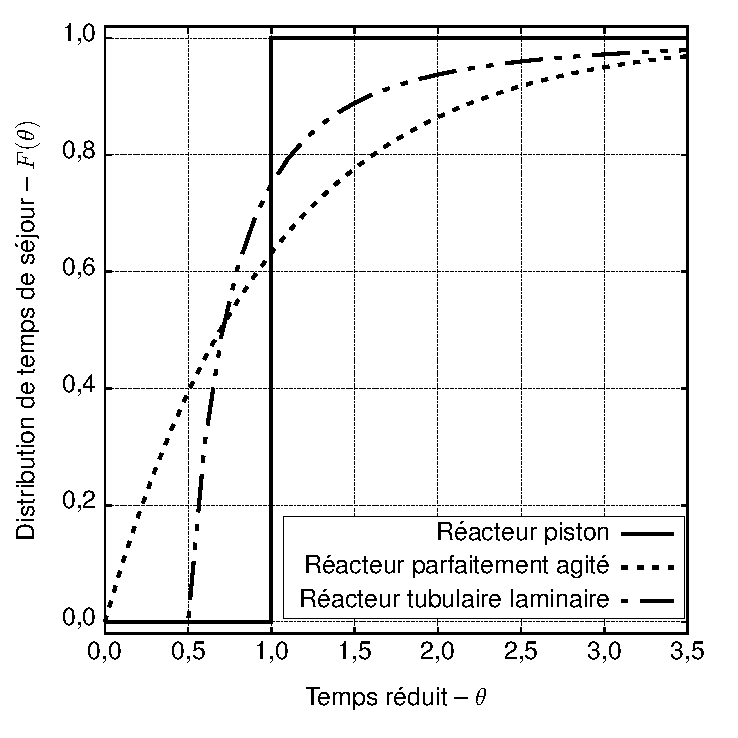
\includegraphics{figures/ch-01-types_de_reacteur}}
  
  \caption{\label{fig:types_de_reacteur}Distribution cumulative de temps de
    séjour en fonction du temps réduit pour différents types de réacteur.}
\end{figure}

\section{Cinétique des processus chimiques}
\label{sec:cinetique}

La connaissance précise du comportement de l'atmosphère carburante/nitrurante est fondamentale pour la maitrise industrielle des procédés thermochimiques.  Selon \citet{Dulcy2007} \og{}\textit{la compréhension des mécanismes de transfert de matière, des mécanismes physicochimiques associés à la réaction gaz-solide et des caractéristiques hydrodynamiques et thermiques des réacteurs a permis de concevoir des procédés permettant d'accroître la productivité par réduction des temps de traitement et corrélativement de réduire la consommation d'énergie}\fg{}.  L'optimisation des procédés thermochimiques est liée à la minimisation des résistances de transport de matière en phase gazeuse, au transfert de matière à l'interface gaz--solide et à l'intérieur du solide. Lorsque l'optimisation hydrodynamique est établie, dans le cas de la carbonitruration par exemple, il reste encore à diminuer la résistance à l'interface pour permettre la saturation de l'austénite en surface~\cite{Dulcy2007}, ce qui pour une nuance donnée représente l'optimum possible du transport à l'état solide.

Cela implique le besoin de traiter les réactions en phase gazeuse et aux interfaces gaz--solide \textendash{} parois du four et matériau traité \textendash{} afin d'améliorer la compréhension et donc le contrôle des mécanismes qui définissent la composition de l'atmosphère.  Un tel contrôle permettrait de prédire l'apport en carbone en fonction des paramètres opératoires du réacteur. Cette section présente les fondements théoriques de la cinétique chimique. Les systèmes cinétiques modélisés seront présentés avec les résultats expérimentaux au Chapitre~\ref{ch:modelisation_cinetique}.

Il faut remarquer que cette approche est valable lorsque le nombre de Knudsen~\cite{Hershey1973} $\varkappa=\nicefrac{\lambda}{L}$, où $\lambda$ est le libre parcours moyen et $L$ une dimension représentative de l'enceinte contenant le gaz, est inférieur à 0,01 \textendash{} donc dans un régime dit visqueux. À partir du moment où $\lambda$ est du même ordre de grandeur que les dimensions $L$ de l'enceinte contenant le gaz, les collisions moléculaires en phase homogène deviennent assez rares et les particules sont soumises principalement à des échanges de quantité de mouvement avec les parois du réacteur. Cette limite de régime possède deux implications fondamentales qui affectent fortement les traitements thermochimiques: comme le transport de masse et la cinétique chimique en domaine homogène dépendent des collisions entre les molécules, leur absence implique l'impossibilité de recourir aux équations des milieux continus pour modéliser le transport et toute modification de l'atmosphère résulte alors des interactions avec les surfaces catalytiques du réacteur. Pour les conditions que nous avons retenues pour la carbonitruration à basse pression (température de l'ordre de \SI{1173}{\kelvin} et pression de \SI{10}{\hecto\pascal}, dans des réacteurs ayant des dimensions de l'ordre de quelques dizaines de centimètres), on estime~\cite{Struchtrup2005} $\lambda\approx{10^{-5}}\ll{L}$ et donc le comportement du milieu peut être considéré comme continu, la description des mécanismes chimiques en phase homogène étant alors nécessaire.

\subsection{Processus homogènes: phase gazeuse}

La grande majorité des réactions chimiques ne donne pas lieu à une transformation directe des réactifs en produits finaux stables. Ces transitions s'opèrent par une série d'étapes intermédiaires faisant intervenir des états transitoires. Chacune de ces interactions est une réaction élémentaire~\cite{Green2007,Henriksen2008}. Un traitement détaillé des fondements physiques de ce sujet est disponible dans l'ouvrage de \citet{Henriksen2008}. Les réactions élémentaires conduisent en général à l'expression de lois de vitesse ayant des ordres entiers et identiques aux coefficients st{\oe}chiométriques des espèces participant à la réaction. Pour ce type de lois de vitesse dites élémentaires~\cite{Fogler1999}, les coefficients cinétiques possèdent un sens physique~\cite{Henriksen2008}.

Plusieurs logiciels et codes de simulation numérique existent pour fournir la solution de l'évolution de systèmes cinétiques chimiques. Même si plusieurs autres méthodes d'intégration de ces systèmes existent~\cite{Berberan1990, Park201342,Parumasur2005473,Bizetti2012}, on traitera la modélisation des réactions chimiques en phase gazeuse selon l'approche typique employée par la plupart des logiciels existant~\cite{Premix1998,Chemkin2000,Transport2000, SurfaceChemkin2000,Damian20021567,DetchemKin,Tchem2011,Cantera2014} dont le caractère général de la formulation est un avantage. Le problème se résume typiquement à résoudre un ensemble d'équations différentielles non--linéaires couplées, comprenant une équation pour chaque espèce chimique et une équation pour chaque variable thermodynamique indépendante. Étant donnés les écarts importants qu'il peut y avoir entre les échelles de temps pour les différents processus qui se déroulent simultanément, la solution numérique d'un tel système d'équations demande souvent l'emploi d'une méthode implicite~\cite{Coles2011} ou utilisant des intégrateurs à pas multiples, comme cela est proposé par les librairies Tchem~\cite{Tchem2011} et Cantera~\cite{Cantera2014} qui utilisent CVode~\cite{Hindmarsh2005}.

La description des vitesses de réaction adoptée dans le présent travail trouve ses fondements dans la loi d'action de masse~\cite{Landau1980}.  Cette formulation décrit l'équilibre chimique à travers des vitesses de processus directs et indirects qui doivent être les mêmes, permettant ainsi le calcul de la constante d'équilibre. Étant donnée la nature statistique de cette loi, les transformations sont dépendantes des pressions partielles \textendash{} \emph{i.e.} des quantités de matière \textendash{} des espèces participant à la réaction considérée. Pour introduire cette formulation, supposons une réaction élémentaire comme \ch{$\nu_{A}$ A + $\nu_{B}$ B <=> $\nu_{C}$ C + $\nu_{D}$ D}. La constante d'équilibre $K_{p}$ à une température donnée de cette réaction en termes de pressions partielles des espèces est fournie par l'Équation~\ref{eq:equilibrium_constant} qui la généralise. % en termes des coefficients st{\oe}chiométriques. %Le produit à droite dans cette expression, qui généralise la définition de $K_{p}$, laisse entendre implicitement que les coefficients st{\oe}chiométriques $\nu_{i}$ des réactifs sont de signe négatif et ceux des produits positifs. %Cela sera important plus tard quand on réalisera le bilan matière pour obtenir le taux d'avancement d'une réaction.

\begin{equation}
  K_{p}(T)=
  \frac{P_{C}^{\nu_{C}}P_{D}^{\nu_{D}}}{P_{A}^{\nu_{A}}P_{B}^{\nu_{B}}}=
  \prod_{i}P_{i}^{\nu_{i}}
  \label{eq:equilibrium_constant}
\end{equation}

Cette constante peut aussi être écrite en termes de concentrations des espèces à une pression totale $P$ donnée, ce que l'on note $K_{c}$ (Équation~\ref{eq:equilibrium_constant_concentration}).  Il faut remarquer que la dépendance de la constante d'équilibre $K_{c}$ avec la pression est liée au facteur $P^{-\sum\nu_{i}}$, où $\sum\nu_{i}$ représente le bilan molaire de la réaction. Considérons par exemple la décomposition de l'ammoniac, où $K_{c}\propto P^{-2}$, ce qui implique une augmentation de $K_{c}$ lorsque la pression est réduite. De l'équilibre des processus directs et indirects, une telle relation montre que la réduction de pression de \SI{1000}{\hecto\pascal} \textendash{} approximativement la pression atmosphérique \textendash{} à \SI{10}{\hecto\pascal}, typique des traitements thermochimiques à basse pression, mène à une réduction de quatre ordres de grandeur dans la quantité d'ammoniac disponible pour le traitement et donc à de possibles difficultés d'enrichissement en azote.

\begin{equation}
  K_{c}(T)=
  \big(P^{-\sum\nu_{i}}\big)K_{p}(T)=
  \prod_{i}c_{i}^{\nu_{i}}
  \label{eq:equilibrium_constant_concentration}
\end{equation}

On peut donc, à partir de la loi d'action de masse, introduire les taux d'avancement de réaction $\dot{\omega}$ dans chaque sens comme étant de la forme $\dot{\omega}=k\prod c_{i}^{\nu_{i}}$. La constante des processus directs sera notée $k_{f}$, celle des processus indirects $k_{b}$. Pour que la relation d'équilibre selon l'action de masse soit préservée, il faut que $K_{c}=\nicefrac{k_{f}}{k_{b}}$~\cite{Landau1980,Stolen2004}.  Une fois connue la constante cinétique d'un processus chimique, la thermodynamique fournit celle de la réaction indirecte \textemdash{} pour les processus réversibles. Ces constantes présentent, en général, une dépendance exponentielle avec la température qui peut être typiquement exprimée par une loi d'Arrhenius. Les données disponibles dans la littérature se trouvent le plus souvent exprimées sous forme de coefficients pour l'Équation~\ref{eq:reaction_constant}, où $A_{i}$ est le facteur pré--exponentiel lié au temps de vie moyen d'une espèce activée et à la fréquence de collision, $n_{i}$ est l'exposant de température et $E_{a,i}$ l'énergie d'activation, qui représente un seuil énergétique à dépasser pour activer la réaction.

\begin{equation}
  k_{f,i}=
  A_{i}{\biggr(\frac{T}{T_{ref}}\biggr)}^{n_{i}}\exp\left(-\frac{E_{a,i}}{RT}\right)
  \label{eq:reaction_constant}
\end{equation}

À partir de ces notions de processus directs et indirects et de la formulation de la loi d'action de masse en termes de concentrations, on peut écrire l'Équation~\ref{eq:advance_rate} pour le calcul des taux d'avancement de réaction. Cette équation est simplement le bilan entre les vitesses directes et indirectes des réactions.

\begin{equation}
  R_{i}=
  k_{f,i}\prod_{l=1}^{N_{s}}c_{l}^{\nu_{l,i}^{\prime}}-
  k_{b,i}\prod_{l=1}^{N_{s}}c_{l}^{\nu_{l,i}^{\prime\prime}}
  \label{eq:advance_rate}
\end{equation}

Finalement, en faisant le bilan molaire $\Delta{}\nu_{l}=\nu_{l,i}^{\prime\prime}-\nu_{l,i}^{\prime}$ pour l'espèce $l$ en fonction de ses coefficients st{\oe}chiométriques dans toutes les réactions où elle intervient comme produit ($\nu_{l,i}^{\prime\prime}$) et réactif ($\nu_{l,i}^{\prime}$), on obtient sa vitesse molaire de formation $\dot{\omega}_{l}$.  Cela est présenté dans l'Équation~\ref{eq:rate_species_general} qui introduit aussi le facteur $\mathbb{C}_{i}$. 

\begin{equation}
  \dot{\omega}_{l}=
  \sum_{i=1}^{N_{r}}\Delta{}\nu_{l}
  \mathbb{C}_{i}R_{i}
  \qquad\text{où}\qquad
  \mathbb{C}_{i}=
  \begin{cases}
    1 
    & \text{\footnotesize{}(i)}\\[8pt]
    \sum_{l=1}^{N_{s}}\alpha_{l,i}c_{l} 
    & \text{\footnotesize{}(ii)}\\[8pt]
    \dfrac{P_{r,i}}{1+P_{r,i}}F_{i} 
    & \text{\footnotesize{}(iii)}\\[8pt]
    \dfrac{1}{1+P_{r,i}}F_{i} 
    & \text{\footnotesize{}(iv)}
  \end{cases}
 \label{eq:rate_species_general}
\end{equation}

\clearpage

Ce facteur $\mathbb{C}_{i}$  introduit la dépendance avec la pression des processus chimiques. En général sa valeur est unitaire dans le cas (i) des réactions élémentaires \textemdash{} celles qui décrivent directement le processus chimique dans une seule étape. D'autres formulations sont présentées ci-dessous pour les réactions (ii) à trois corps, (iii) unimoléculaires et de récombinaison et (iv) bimoléculaires. % Ces descriptions supplémentaires sont nécessaires à la description des processus dont la formulation élémentaire n'est pas complètement connue ou quantifié~\cite{Green2007}.

Dans le cas d'une réaction simple, $\mathbb{C}_{i}$ est unitaire. Pour les réactions à trois corps, sa valeur représente la concentration effective du troisième corps, où $\alpha_{l,i}$ est l'efficacité du troisième corps pour l'espèce $l$ dans la réaction $i$ et $c_{l}$ sa concentration. Si toutes les espèces interviennent de manière équivalente en tant que troisième corps, les facteurs $\alpha_{l,i}$ sont tous unitaires et la concentration effective est la concentration du mélange.  Les processus de dissociation unimoléculaire et de récombinaison dépendent de la présence d'un troisième corps pour que le bilan énergétique soit possible. Selon la théorie de Lindemann, les vitesses de réaction sont proportionnelles à la concentration de ce troisième corps dans les systèmes dilués et arrivent à une valeur limite lorsque la concentration de ces espèces atteint un seuil.

Dans ce modèle de Lindemann, la pression réduite $P_{r,i}$ est définie par l'Équation~\ref{eq:reduced_pressure}. Par définition, l'efficacité du troisième corps $\alpha_{l,i}$ d'une espèce est unitaire. Si certaines espèces jouent un rôle sur la vitesse de réaction, seules les concentrations de ces espèces sont prises en compte par cette expression. Les constantes $k_{\infty,m}$ dans la limite des pressions élevées et $k_{0,m}$ dans la limite des pressions basses nécessaires à la description des réactions de types \og{}fall-off\fg{} et bimoléculaires activées chimiquement sont données comme des fonctions de la température selon l'Équation~\ref{eq:reaction_constant}. Dans le cas des réactions unimoléculaires et/ou de récombinaison, les paramètres d'Arrhenius de $k_{\infty,m}$ doivent être pris en compte pour le calcul de $k_{f,m}$. Pour les réactions bimoléculaires activées chimiquement, ce sont les valeurs de $k_{0,m}$ qui doivent être utilisées.

\begin{equation}
  P_{r,i}=\frac{k_{0,i}}{k_{\infty,i}}\sum_{k=1}^{N_{s}}\alpha_{l,i}c_{l}
  \label{eq:reduced_pressure}
\end{equation}

La transition entre les régimes de haute et basse pressions est modélisée par l'Équation~\ref{eq:falloff}, où les $a_{i}$, $T_{i}^{***}$, $T_{i}^{*}$ et $T_{i}^{**}$ sont des paramètres du modèle. Il existe d'autres formulations pour la modélisation de cette transition. Cependant, les mécanismes cinétiques employés dans le présent rapport utilisent les paramètres issus du formalisme de Troe.

\begin{equation}
  \log_{10}F_{i}=
  \biggr[1+\biggr(\frac{A}{B}\biggr)^{2}\biggr]^{-1}\log_{10}F_{cent,i}
  \label{eq:falloff}
\end{equation}

\noindent où les facteurs $F_{cent,i}$, $A$ et $B$ sont donnés par : 
\[
\begin{aligned} 
  & F_{cent,i}=
   (1-a_{i})\exp\biggr(-\frac{T}{T_{i}^{***}}\biggr)+
   a_{i}\exp\biggr(-\frac{T}{T_{i}^{*}}\biggr)+
   \exp\biggr(\frac{T_{i}^{**}}{T}\biggr)\\[5pt]
  & A=\log_{10}P_{r,i}-0,67\log_{10}F_{cent,i}-0,4\\[5pt]
  & B=0,806-1,1792\log_{10}F_{cent,i}-0,141\log_{10}P_{r,i}
\end{aligned}
\]

\clearpage

Étant donné le fait que les réactions s'accompagnent d'un changement de l'enthalpie libre du gaz ainsi que de sa masse molaire moyenne, laquelle intervient dans la concentration des espèces, l'ensemble des équations cinétiques ainsi écrites doit être fermé par une équation d'état. Cela se fait le plus souvent à l'aide de la loi des gaz parfaits donnée par l'Équation~\ref{eq:ideal_gas_law}.
%~\footnote{Les concentrations $c_{l}$ sont définies par le rapport entre le nombre de moles $N_{l}$ d'une espèce et le volume $V$ occupé par le système, $c_{l}=\nicefrac{N_{l}}{V}=\rho\nicefrac{Y_{l}}{M_{l}}$ -- où $\rho$ désigne la masse volumique et $Y_{l}$ la fraction massique relative à l'espèce de masse molaire $M_{l}$.}

\begin{equation}
  \rho=\frac{PM}{RT}\quad\text{où}\quad
  M=\sum_{i=1}^{N_{s}}X_{i}M_{i}=
  \biggr(\sum_{i=1}^{N_{s}}\frac{Y_{i}}{M_{i}}\biggr)^{-1}
  \label{eq:ideal_gas_law}
\end{equation}

Le changement de température dans le système est donné par l'Équation~\ref{eq:enthalpy_change}, où l'enthalpie molaire $h_{i}$ de l'espèce $i$ est calculée à partir d'un polynôme~\cite{Tchem2011}. Comme les procédés sont réalisés à pression constante, la dérivée de la pression au cours du temps est égale à zéro. Dans ce cas, si l'on simule un système fermé à volume variable, l'équation de la densité (ou du volume) doit être ajoutée au système d'équations différentielles à intégrer.

\begin{equation}
  \frac{\mathrm{d}T}{\mathrm{d}t}=
  -\frac{1}{\rho c_{p}}\sum_{i=1}^{N_{s}}h_{i}\dot{\omega}_{i}
  \label{eq:enthalpy_change}
\end{equation}

\subsection{Processus hétérogènes: interfaces solides}

Alors que la cinétique en phase gazeuse contrôle l'arrivée des précurseurs des traitements thermochimiques jusqu'aux surfaces des pièces à enrichir, ce sont les réactions hétérogènes qui apportent de la matière au solide. Cela n'est valable que si le nombre de Knudsen~\cite{Hershey1973} traduit un comportement visqueux, comme discuté au début de cette section. Sans quoi, la cinétique de surface gouverne le procédé. Ce n'est en général pas le cas à des pressions supérieures à \SI{1}{\hecto\pascal} comme cela a lieu dans les traitements de cémentation et de  nitruration des aciers. Par conséquent la compréhension des phénomènes d'enrichissement demande l'intégration simultanée des cinétiques homogènes et hétérogènes. Les vitesses des réactions hétérogènes doivent être proportionnelles aux flux nets des espèces participant aux réactions, lesquels sont orientés vers les surfaces. Cela comprend les flux par agitation thermique, diffusion, advection et accélération par des champs externes. En l'absence de champs, les vitesses des transports par advection et diffusion (de l'ordre de quelques \si{\metre\per\second})~\cite{Bird,Atkins2006} sont négligeables par rapport aux vitesses d'agitation thermique. On suppose donc que la vitesse de réaction ne dépend que de ce terme. La vitesse thermale moyenne $\bar{v}_{th}$ d'une espèce de masse molaire $M$ dans un gaz à température $T$ est donnée par l'Équation~\ref{eq:thermal_velocity}.

\begin{equation}
  \bar{v}_{th}=\biggr(\frac{8RT}{\pi{M}}\biggr)^{\nicefrac{1}{2}}
  \label{eq:thermal_velocity}
\end{equation}

L'Équation~\ref{eq:thermal_velocity} met en évidence une plus grande mobilité des espèces légères et donc l'influence plus prononcée de ces espèces sur les processus hétérogènes. On peut montrer à partir de la mécanique statistique~\cite{Atkins2006} que le flux $J_{i}$ d'une espèce $i$ par unité de surface est donné par l'Équation~\ref{eq:surface_flux}, où $\mathcal{N}_{i}$ désigne la concentration des molécules. Il est intéressant de noter dans cette formulation que l'effet de la température sur la masse volumique du gaz est prépondérant par rapport à son effet sur la vitesse moyenne des molécules.

\clearpage

\begin{equation}
  J_{i}=\frac{1}{4}\bar{v}_{th}\mathcal{N}_{i}=
  \frac{p_{i}N_{A}}{(2\pi{MRT})^{\nicefrac{1}{2}}}
  \label{eq:surface_flux}
\end{equation}

Ainsi, à basse pression partielle de précurseurs et à températures élevées, on doit s'attendre à que les flux d'espèces vers la surface soient faibles. Le taux d'adsorption dépend de la capacité du substrat à dissiper l'énergie de la particule arrivant; si la surface se trouve à haute température, il est très probable que l'adsorption n'ait pas lieu compte tenu des vibrations dans le solide. La probabilité d'adsorption, définie comme le rapport entre le taux d'adsorption et le flux de particules qui subissent une collision avec la surface reste faible. En outre, les processus de désorption ont des temps caractéristiques de l'ordre de \SIrange{10}{100}{\femto\second} et donc, la probabilité de recombinaison par diffusion en surface des espèces sorbées reste très faible ainsi que le taux de couverture $\theta$ de l'interface~\cite{Atkins2006}. Par conséquent, la contribution des processus de surface au changement de la composition dans le volume $V$ de l'atmosphère peut être exprimée globalement comme étant proportionnelle au flux des réactifs selon l'Équation~\ref{eq:rate_surface}, où $k_{w}$ désigne la constante de réaction et $S$ la surface traitée. 

\begin{equation}
V\frac{\mathrm{d}c_i}{\mathrm{d}t}=-k_{w}S{J_{i}}
\label{eq:rate_surface}
\end{equation}

Cette formulation suppose que le nombre de sites réactifs est intégré dans la constante de réaction $k_{w}$. En outre, comme les traitements étudiés ici sont réalisés sur des surfaces polycristallines sans orientation préférentielle, cette constante n'est qu'une moyenne globale sans aucun sens physique. Dans le cas plus général et complet de la description des processus de surface, différents types de sites sont disponibles pour les réactions hétérogènes en fonction des différents plans cristallins du matériau traité~\cite{Alcock2001}. 

Il faut remarquer qu'une telle description de processus traités de manière globale implique l'existence d'une température optimale au--delà de laquelle l'enrichissement des matériaux par voie thermochimique n'est pas favorable en raison de limitations cinétiques de surface: le transfert de matière est limité par le faible degré d'adsorption et par des conditions favorables à la désorption. Dans le cas des traitements à basse pression pour lesquels les temps de séjour dans l'enceinte du four deviennent assez courts, la conversion des précurseurs en phase gazeuse sera limitée, ce qui peut être à l'origine de difficultés d'enrichissement des surfaces.% traitées.  

\subsection{Simplification des mécanismes cinétiques}
\label{sec:simplification_cinetique_lu_and_law}

Comme cela a été défini tout au début de cette section, les processus chimiques élémentaires portent des informations relatives à la physique du système, tout en gardant aussi les relations d'interdépendance entre les espèces: les étapes élémentaires de réaction passant par des états de transition sont ainsi représentées.  En général, les mécanismes élémentaires comprennent des centaines ou même des milliers d'espèces chimiques, ce qui conduit à des ensembles de réactions de tailles similaires. Quelques exemples sont donnés par \citet{Coles2011}. Comme chaque espèce évolue au cours du temps, la modélisation en régime transitoire des écoulements réactifs \textendash{} comme c'est le cas pour les traitements thermochimiques à basse pression pendant toute la durée du traitement \textendash{} requiert d'ajouter une équation par espèce au système à résoudre.  Cela se fait le plus souvent en utilisant la méthode CFD~\footnote{De l'Anglais \textit{Computational Fluid Dynamics}.}~\cite{Liang2009} et plus récemment à l'aide de la méthode dite de Boltzmann sur réseau~\cite{Li20131194,Sullivan2006206} (LBM). Étant donné le grand nombre d'espèces typiquement présentes dans les modèles cinétiques détaillés, comme celui de \citet{Norinaga2009}, ces simulations sont généralement limitées en termes de temps de calcul, même avec les ordinateurs disponibles aujourd'hui. 

La modélisation de la pyrolyse et de la combustion des hydrocarbures atteint facilement des centaines, voire des milliers de réactions. Un mécanisme offrant une grande précision pour des courts temps de séjour et relatif à la pyrolyse 
%\textendash{} décomposition homogène \textendash{}
de l'acétylène a été proposé dans la littérature par \citet{Norinaga2007,Norinaga2007ii}.  Il a été validé expérimentalement par \citet{Norinaga2005} puis amélioré pour inclure des espèces de hauts poids moléculaires~\cite{Norinaga2009} pour arriver finalement à plus de 240 espèces et 900 réactions. La simulation directe d'écoulements réactifs qui inclurait un modèle aussi complet de la phase gazeuse n'est pas possible. Il faut tout d'abord obtenir une version simplifiée du schéma cinétique en ne gardant que les espèces du système présentant un intérêt pour l'application recherchée. Aucune méthode existant ne permet l'obtention d'un tel \og{}squelette\fg{} de mécanismes pour n'importe quel ensemble de conditions initiales. Dans le cas du système \ch{N-H} pour l'ammoniac, le mécanisme~\cite{Dirtu2006,Odochian2011} adopté est suffisamment simple pour être utilisé dans des calculs de CFD.

Avant de décrire la méthode de simplification adoptée pour inclure un modèle cinétique simplifié dans une simulation d'écoulement réactif, il convient de comprendre la différence entre réduction et simplification des modèles cinétiques. La réduction consiste en une procédure mathématique de diminution de la rigidité du système d'équations des espèces et des variables thermodynamiques considérées, rendant la solution du problème plus stable et convergente. Pour l'obtention des mécanismes squelettes, on parle de simplification : cela consiste à diminuer le nombre d'espèces et de réactions du système, en gardant les espèces majoritaires \textendash{} dont la connaissance préalable du comportement empirique lors de la pyrolyse est requise \textendash{} et celles aussi qui sont en forte interaction avec les espèces majoritaires~\cite{Coles2011}.

Plusieurs méthodes de simplification existent, comme l'analyse de sensibilité de \citet{Turanyi1989} et les hypothèses classiques des états quasi--stationnaires et d'équilibre partiel. Une comparaison entre plusieurs méthodes existantes a été effectuée par \citet{Coles2011}.  Dans le présent travail, on se limitera aux développements conduits par \citet{Lu2005} et aux applications et/ou améliorations proposées~\cite{Lu2006i,Lu2006ii,Pepiot2008}.  Ces méthodes ont comme caractéristique commune le besoin d'une connaissance préalable du comportement chimique du système. Plus récemment \citet{Curtis2015} ont proposé une implémentation à partir de la méthode de \citet{Pepiot2008} avec une sélection automatique des espèces. En outre, la méthode DRG~\footnote{De l'Anglais, Directed Relational Graph method.} de \citet{Lu2005} est très simple  à implémenter numériquement comparée à celle (CSP~\footnote{De l'Anglais, Computational Singular Perturbation method.}) de \citet{Lam1993,Lam1994}. Une utilisation de cette méthode dite des graphes de liaisons orientés de \citet{Lu2005} pour des simulations CFD est présentée par \citet{Liang2009} et s'avère satisfaisante.  La méthode de perturbation CSP de \citet{Lam1994} est utilisée avec succès par \citet{Ortega2007}. Une approche modifiée par \citet{Curtis2015} permet l'obtention automatique de mécanismes simplifiés en simulation avec une chimie adaptative.

\clearpage

La méthode~\cite{Lu2005} consiste en la construction d'un graphe de liaisons orientées entre espèces placées aux n{\oe}uds du graphe et les arêtes sont affectées d'un coefficient d'interaction $r_{ij}$ relatif aux espèces connectées ($i\rightarrow j$). Les ouvrages de \citet{Bondy1976} et \citet{Diestel2000} présentent des aspects de la théorie des graphes et de l'algorithme de recherche utilisé dans la méthode de simplification adoptée. Du fait que l'on considère le graphe orienté la matrice d'adjacence n'est pas symétrique, $r_{ij}\neq r_{ji}$, \textit{i.e.} l'espèce $i$ intervient sur la vitesse de formation de $j$ d'une manière différente de celle dont $j$ affecte $i$. Ce coefficient d'interaction $r_{ij}$ représente l'erreur sur le taux de formation de $j$ si l'on supprime $i$ du mécanisme et est défini par l'Équation~\ref{eq:coefficient_interaction}, où les paramètres ont les définitions fournies section précédente.  Le symbole de Kronecker $\delta_{jk}$ vaut l'unité si l'espèce $j$ est présente dans la réaction $k$ et zéro autrement.

\begin{equation}
  r_{ij}\equiv
  \dfrac{
   \sum_{k}^{N_{s}}\vert\nu_{i,k}\omega_{i}\delta_{jk}\vert}{
   \sum_{k}^{N_{s}}\vert\nu_{i,k}\omega_{i}\vert}
  \label{eq:coefficient_interaction}
\end{equation}

Si la valeur du coefficient est plus grande qu'un certain $\varepsilon$ défini avant la réduction, la suppression de $j$ du mécanisme produit un effet non--négligeable sur $i$. Donc, si $i$ doit être conservé dans le mécanisme, $j$ doit l'être aussi. En suivant cette logique, un graphe du système est construit de telle façon que l'arête $i\rightarrow j$ n'existe que si $r_{ij}\geq\varepsilon$. Une fois le graphe établi, on s'en sert comme algorithme de parcours en profondeur en partant des n{\oe}uds qui représentent les espèces choisies préalablement. Toutes les espèces retrouvées au cours de ce parcours sur le graphe sont retenues dans le mécanisme simplifié. Après identification de cet ensemble d'espèces, on élimine les réactions contenant d'autres espèces que celles retenues dans l'étape précedente. De cette façon, on obtient ainsi un mécanisme squelette. Il faut remarquer que le choix de $\varepsilon$ joue un rôle important sur la précision du mécanisme squelette. L'intersection de plusieurs réductions dans l'espace des états connus empiriquement produit des mécanismes avec une précision supérieure mais présentant l'inconvénient d'agréger plus d'espèces. Cette approche sera employée Chapitre~\ref{ch:modelisation_cinetique} pour l'obtention des mécanismes simplifiés à partir du mécanisme général de \citet{Norinaga2009}.

\clearpage\section{Conclusion}

Le Chapitre~\ref{ch:aspects_procedes} fait le point sur les aspects procédés liés aux traitements thermochimiques des aciers faiblement alliés. Les fondements qui y sont présentés servent de base aux discussions qui seront conduites dans les Chapitres~\ref{ch:caracterisation_atmospheres}~et~\ref{ch:modelisation_cinetique} et peuvent être résumés ainsi:
\begin{itemize}
  \item le contrôle des procédés de cémentation utilisant \ch{CO-H2} peut être réalisé à partir de diagrammes de températures de point de rosée. C'est aussi le cas pour les procédés de nitruration grâce aux diagrammes de potentiel de nitruration. Ces expressions sont disponibles pour le fer. Cette démarche peut être généralisée en utilisant la thermodynamique numérique;
  
  \item la diffusion du carbone et de l'azote à l'état solide dans des alliages à base de fer dépend des interactions entre les interstitiels et leur environnement métallurgique. Pour les systèmes plus simples, l'introduction d'une dépendance des coefficients de diffusion avec la composition peut être adoptée, mais pour les alliages \og{}réels\fg{}, l'approche formelle d'\citet{Onsager1931,Onsager1931ii} est nécessaire;
  
  \item la maîtrise des conditions aux limites pour les enrichissements en carbone et en azote nécessite un contrôle précis de l'atmosphère de traitement. Comme il n'est pas toujours possible de modéliser les réacteurs industriels par des approches limites de type réacteur \og{}agité\fg{} ou réacteur \og{}piston\fg{}, des mesures de la distribution de temps de séjour peuvent être utilisées pour prédire le degré de conversion des précurseurs dans les chambres de traitement;
  
  \item pour un suivi précis des atmosphères que l'on peut décrire comme des milieux continus, la modélisation de la cinétique détaillée doit être réalisée de manière couplée à l'écoulement et aux échanges thermiques dans le réacteur. Bien que cette approche permette le calcul du bilan énergétique interne grâce aux étapes élémentaires de la chaine de réactions, \emph{i.e} il possède une cohérence thermodynamique, son utilisation pour le suivi en temps réel et mise au point des réacteurs industriels est limitée par le grande nombre d'espèces et de réactions à considérer, ce qui couplé à la mécanique des fluides impose une contrainte en termes de temps de calcul. L'obtention de mécanismes simplifiés permet donc d'échantillonner l'ensemble des réactions et des espèces qu'il convient de retenir pour une région spécifique de l'espace des états et donc de réaliser des simulations de réacteurs réels dans un délai raisonnable pour des applications industrielles.  
\end{itemize}

\endinput
  \cleardoublepage\chapter{Approche métallurgique }
\label{ch:thermodynamique}

\vfill

Ce chapitre vise à présenter les caractéristiques et les comportements métallurgiques des alliages 16NiCrMo13 et 23MnCrMo5 sous différentes conditions de traitement et d'enrichissement. La Section~\ref{sec:thermocalc} permet de présenter rapidement l'approche CALPHAD et le logiciel Thermo-Calc~\cite{Andersson2002,Borgenstam2000}. Ce logiciel sera ensuite employé dans l'étude des systèmes binaires et ternaires \ch{Fe-C}, \ch{Fe-N} et \ch{Fe-C-N} à la Section~\ref{sec:simple_systems}, qui présente aussi leur description fournie dans la littérature. Quelques résultats concernant le calcul de diagrammes de phase pour des aciers faiblement alliés sont regroupés dans la Section~\ref{sec:low_alloy} avant de procéder dans la Section~\ref{sec:studied_alloys} aux simulations des diagrammes utiles à la compréhension des nuances étudiées. Les compositions nominales en pourcentage massique de ces alliages sont présentées Tableau~\ref{tab:composition_alliages}. Comme il s'agit d'aciers faiblement alliés, la définition des conditions aux limites pour ces simulations demande la connaissance de la thermodynamique des systèmes contenant non seulement fer, carbone et azote mais aussi nickel, chrome, manganèse et molybdène. Des résultats expérimentaux de la littérature sont nécessaires pour une simulation cohérente des systèmes métallurgiques. Ces données de base seront utilisées au cours des discussions conduites au Chapitre~\ref{ch:reponse_metallurgique}. Alors que l'enrichissement des alliages a été effectué dans des conditions favorisant l'équilibre thermodynamique, les caractéristiques mécaniques des traitements de cémentation et carbonitruration résultent d'une trempe et par conséquent d'une transformation hors équilibre du type martensitique. La Section~\ref{sec:martensite_cn} traite des propriétés obtenues et des caractéristiques métallurgiques des structures martensitiques des aciers au carbone et à l'azote. Finalement la Section~\ref{sec:carbonitrurationalliages} présente des résultats relatifs à la réponse métallurgique et mécanique des aciers faiblement alliés aux traitements thermochimiques de cémentation et de carbonitruration. Cela comprend non seulement des aspects relatifs à la structure, mais aussi des aspects liés à la composition locale des couches enrichies.

\begin{table}[!hb]
  \caption{\label{tab:composition_alliages}Composition nominale en pourcentage massique des alliages étudiés.}
  
  \centering{}\footnotesize{}%
  \begin{tabular}{\$c^c^c^c^c^c^c^c}
    \toprule[2pt] 
    \rowstyle{\bfseries}
    Alliage & Fe & C & Si & Mn & Cr & Ni & Mo\tabularnewline
    \midrule[2pt] 
    16NiCrMo13 & bal. & 0,16 & 0,25 & 0,45 & 1,00 & 3,20 & 0,25
    \tabularnewline[6pt] 
    23MnCrMo5 & bal. & 0,23 & 0,25 & 1,30 & 1,20 & 0,10 & 0,25
    \tabularnewline
    \bottomrule
  \end{tabular}
\end{table}

\vfill\clearpage

\section{L'approche CALPHAD et Thermo-Calc}
\label{sec:thermocalc}

Les premiers travaux sur les transformations de phase des aciers faiblement alliés remontent aux années 1930. À partir de ces résultats pionniers, d'énormes progrès ont été réalisés. Ce n'est qu'avec les initiatives de Kaufmann et Ansara, qui sont à l'origine de l'approche CALPHAD~\footnote{Originalement de l'Anglais \textit{CALculation of PHAse Diagrams}, Calcul des Diagrammes de Phase. Aujourd'hui la communauté CALPHAD s'intitule \textit{Computer Coupling of Phase Diagrams and Thermochemistry}, Couplage Numérique du Calcul des Diagrammes de Phase et Thermochimie.}, dans les années 1970 que le calcul des diagrammes de phase avec l'aide d'ordinateurs est devenu populaire~\cite{Spencer2007}. Dans cette méthode, l'énergie de Gibbs de chaque phase est exprimée en fonction de la température, de la composition et, parfois de la pression. À partir de ces données, qui sont généralement issues des mesures expérimentales, l'équilibre est calculé en minimisant numériquement l'énergie libre. Le plus souvent la représentation de ces données thermodynamiques est faite en utilisant des polynômes de Redlich-Kister~\cite{Redlich1948,Hillert2008}. Plusieurs modèles de solution solide sont disponibles pour que l'équilibre soit calculé, parmi lesquels on trouve le modèle classique de Bragg-Williams des solutions strictement régulières~\cite{Hillert2008}. Pour des phases st{\oe}chiométriques le modèle des solutions régulières de \citet{Hillert1970} est le plus connu. Ce sont ces modèles qui sont incorporés dans l'approche CALPHAD que l'on trouve dans le logiciel Thermo-Calc~\cite{Andersson2002,Borgenstam2000} utilisé dans la présente étude. Ce logiciel est utilisé dans la simulation des systèmes thermodynamiques formés par plusieurs groupes de matériaux, sa description détaillée étant disponible dans des publications de \citet{Sundman1985} et \citet{Andersson2002}. L'ouvrage de \citet{Hillert2008} résume globalement les fondements théoriques nécessaires à son utilisation.

Alors que l'utilisation d'un logiciel de ce type permet d'obtenir rapidement des résultats sur les matériaux ou les traitements étudiés, il est aussi facile d'obtenir des informations sans sens physique sur les phénomènes modélisés. Une connaissance préalable des phases possiblement attendues à l'équilibre dans des conditions réalistes de simulation est indispensable avant de procéder à des calculs. Pour cette raison, la suite de ce chapitre est consacrée à réunir des résultats de la littérature permettant une utilisation correcte de Thermo-Calc~\cite{Andersson2002,Borgenstam2000}. L'intérêt principal d'utiliser un logiciel prédisant les équilibres thermodynamiques pour l'étude et la mise au point de traitements thermochimiques est de prédire la formation des précipités qui apparaissent lors du traitement, ce qui induit une consommation des éléments d'alliage de la matrice austénitique que l'on peut observer par microscopie électronique en transmission. Cela permet également de simuler les limites de solubilité des phases dans les alliages en fonction des teneurs en éléments interstitiels et d'estimer les fractions de phases à une température donnée. Il est aussi possible  de déterminer les facteurs thermodynamiques pour le transport à l'état solide. La connaissance des fractions des éléments d'alliage consommés lors de l'enrichissement des matériaux en carbone et principalement en azote est nécessaire pour comprendre d'abord la réponse mécanique \textendash{} en dureté \textendash{} lors de la trempe, et pour estimer ensuite les possibles équilibres de phases lors du revenu. Comme la formation de ces précipités \og piège \fg{} des éléments interstitiels et conduit aussi à appauvrir la matrice en éléments d'alliage, la réponse au revenu des aciers faiblement alliés peut se rapprocher de celle du fer pur, comme cela sera discuté dans la Section~\ref{sec:carbonitrurationalliages}. Ce type de précipitation à haute température produit une barrière à la diffusion du carbone et de l'azote, ce qui peut être traité par Thermo-Calc~\cite{Andersson2002,Borgenstam2000}. En ce qui concerne le contrôle des procédés, le logiciel permet de généraliser les méthodes présentées dans la Section~\ref{sec:procedes} \textendash{} le calcul des diagrammes de température de point de rosée et de potentiel de nitruration \textendash{} pour des systèmes métallurgiques contenant plusieurs composants chimiques. Pour ces simulations, on se servira des bases de données TCFE7, SSOL4, SSUB3 de Thermo-Calc~\cite{Andersson2002,Borgenstam2000}. On peut résumer les applications de cette approche dans ce rapport au calcul:
\begin{itemize}
  \item des diagrammes de phase binaires,
  \item des sections pseudo-binaires des alliages,
  \item des sections isothermes des alliages,
  \item des diagrammes de potentiel de nitruration,
  \item des diagrammes de température de point de rosée, et
  \item des profils de diffusion-précipitation.
\end{itemize}

\section{Équilibre des phases: résultats de la littérature}
\label{sec:low_alloy_literature}

\subsection{Systèmes modèles: \ch{Fe-C}, \ch{Fe-N} et \ch{Fe-C-N}}
\label{sec:simple_systems}

La description des alliages à base de fer commence avec celles des systèmes connus les plus simples : les diagrammes d'équilibre \ch{Fe-C}, \ch{Fe-N} et \ch{Fe-C-N}. En fait, pour des raisons cinétiques, l'équilibre \ch{Fe-C} n'est normalement pas atteint et le système représentatif pour les aciers est en fait celui du diagramme binaire métastable \ch{Fe-Fe3C}~\cite{Mittemeijer2010} dans lequel le carbone se trouve soit en solution solide avec le fer \textendash{} de limite de solubilité très faible à basse température \textendash{} soit sous forme de cémentite. Ce diagramme (Figure~\ref{fig:binaire_fe_c}) présente les domaines monophasés de la ferrite de structure cubique centrée (CC) connue comme phase $\alpha$ et stable à basse température, de l'austénite $\gamma$ cubique face centrée (CFC) stable à des températures intermédiaires, de la cémentite \ch{Fe_{3}C} et de la phase $\delta$ qui est aussi \og{}CC\fg{} comme la phase $\alpha$ mais se situe près de la température de fusion et dont l'importance technologique est limitée. La simulation de ce diagramme a été réalisée avec les bases de données TCFE7 et SSOL4 conduisant à des résultats assez similaires en termes de domaines de phase représentés graphiquement sur la Figure~\ref{fig:binaire_fe_c}.

Pour la cémentation, les frontières entre les domaines $\alpha+\gamma$ ($\mathrm{A_{3}}$) et $\gamma+\ch{Fe3C}$ ($\mathrm{A_{cm}}$) avec le domaine monophasé de l'austénite sont d'une importance cruciale : la première frontière détermine la température minimale pour conduire le traitement \textendash{} une ligne équivalente peut être calculée pour les systèmes faiblement alliés \textendash{} tandis que la seconde fixe la fraction massique en carbone pour atteindre la saturation de l'austénite et est donc liée au contrôle des atmosphères d'enrichissement. C'est l'activité du carbone sur cette limite $\mathrm{A_{cm}}$ qu'on a calculée à la Section~\ref{sec:controle_cementation}, pour laquelle on observe Figure~\ref{fig:binaire_fe_c} une limite de solubilité dans l'austénite de l'ordre de $w_{s,C}\approxeq0,013$ dans la plage de température typique de la carbonitruration. Cette saturation de l'austénite conduit à la formation de carbures du type \ch{Fe3C}. Si l'on considère encore ce diagramme pour prédire le comportement lors d'un revenu réalisé à \SI{573}{\kelvin} après une trempe, c'est encore \ch{Fe3C} qui est le carbure d'équilibre.

\begin{figure}[h]
  \centering
  \subfloat[\label{fig:binaire_fe_c}\ch{Fe-Fe3C}]{
    \centering
    \resizebox{0.48\textwidth}{!}{
      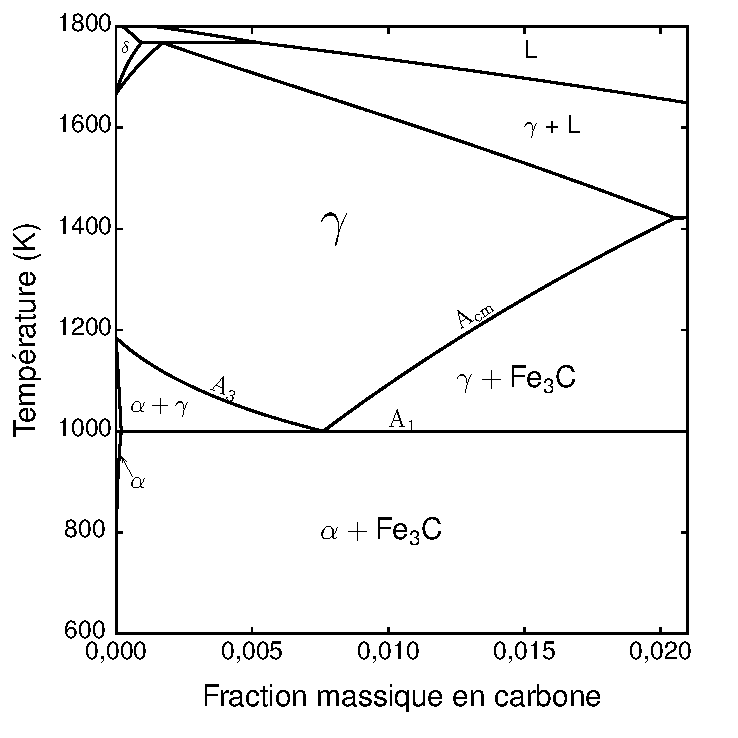
\includegraphics{figures/ch-02-diagram_fe_cem}}
  }\hfill
  \subfloat[\label{fig:binaire_fe_n}\ch{Fe-N}]{
    \centering
    \resizebox{0.48\textwidth}{!}{
      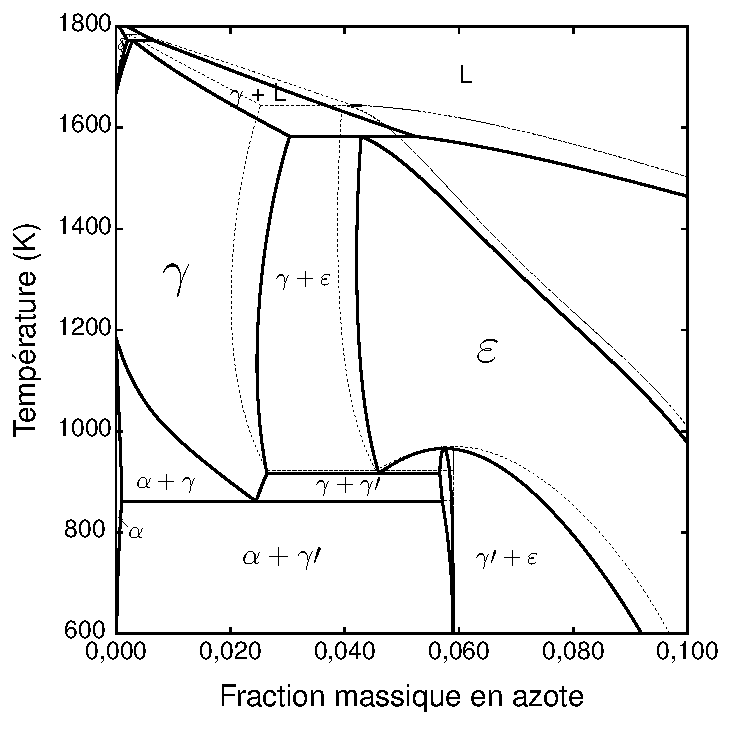
\includegraphics{figures/ch-02-diagram_fe_n}}
  }
  
  \caption{\label{fig:binaires_fe}Diagrammes binaires des systèmes \protect\subref{fig:binaire_fe_c} \ch{Fe-Fe3C} et \protect\subref{fig:binaire_fe_n} \ch{Fe-N}. Thermo-Calc~\cite{Andersson2002,Borgenstam2000}. Traits pleins base de données SSOL4, pontillés TCFE7. Les résultats pour les deux bases de données se superposent dans le diagramme \ch{Fe-Fe3C}.}
\end{figure}

Dans le cas du système \ch{Fe-N} les phases $\alpha$, $\gamma$ et $\delta$ constituent les domaines monophasés \textendash{} avec l'azote comme élément en solution interstitiel \textendash{} auxquels il faut ajouter $\gamma\prime$, phase intermétallique \ch{Fe4N_{(1-x)}} non-st{\oe}chiométrique de structure \og{}CFC\fg{} et $\varepsilon$, intermétallique \ch{Fe2N_{(1-x)}} non-st{\oe}chiométrique de structure hexagonale compacte \og{}HC\fg{}~\cite{Frisk199179,Du1993,Gantois2010}. La Figure~\ref{fig:binaire_fe_n} présente les phases en équilibre de \SIrange{600}{1800}{\kelvin}. On observe dans ce cas des résultats distincts selon la base de données utilisée, notamment une réduction du domaine monophasé $\gamma$ pour la base de données TCFE7, pour laquelle le nitrure \ch{Fe4N} est aussi considéré comme étant st{\oe}chiométrique. Dans la plage de températures employées pour la carbonitruration, l'allure de ce diagramme est semblable à celle observée dans le système \ch{Fe-Fe3C}. Comme pour le système \ch{Fe-Fe3C}, deux lignes dans le diagramme sont particulièrement importantes pour les traitements en phase austénitique : la limite $\alpha+\gamma/\gamma$ détermine la température minimale pour le procédé tandis que la frontière $\gamma/\gamma+\varepsilon$ donne la saturation en azote, qui est située au-delà de la saturation en carbone dans ce cas (une fraction massique de l'ordre de 0,025 en azote).

Pour le système ternaire \ch{Fe-C-N}, les mêmes configurations que celles trouvées dans les binaires sont possibles, auxquelles il faut ajouter la présence des domaines biphasés $\ch{Fe3C}+\varepsilon$ et $\alpha+\varepsilon$, comme cela est exposé dans \citet{Gantois2010}. En faisant un parallèle avec la discussion conduite sur l'étape de revenu dans le système \ch{Fe-Fe3C}, on s'attend à une précipitation de \ch{Fe4N_{(1-x)}} à \SI{573}{\kelvin} pour le système \ch{Fe-N}. Bien que cette phase soit observée expérimentalement, la formation de nitrures intermédiaires de type \ch{Fe16N2}~\cite{Liu2000} est amplement rapportée dans la littérature~\cite{Kaplow1983,vanGent1985,Mittemeijer1988,Cheng199013,Cheng19902857,Fall1996,vanGenderen1997,Sherby2008}. Ces nitrures se forment lors du vieillissement à température ambiante et se décomposent en \ch{Fe4N_{(1-x)}} lors du revenu des alliages \ch{Fe-N}. On reviendra sur ce sujet au Chapitre~\ref{ch:reponse_metallurgique}.

À partir de cette compilation de résultats, et pour simuler les systèmes \ch{Fe-C} et \ch{Fe-N} dans les conditions qui nous intéressent pour les traitements thermochimiques, il faut retenir les phases~\footnote{En raison des modèles de solution utilisés dans le formalisme CALPHAD, les phases à considérer dans une simulation sont décrites par leurs structures cristallines et par les différents sites disponibles dans les réseaux. Cela implique normalement que l'on doit fournir à Thermo-Calc~\cite{Andersson2002,Borgenstam2000} les structures selon leurs nomenclatures utilisées par ces bases de données et non nécessairement par leurs nomenclatures d'usage.} suivantes dans les calculs d'équilibre:
\begin{itemize}
  \item $\alpha$, allotropie \og{}CC\fg{} du fer stable à la température ambiante,
  \item $\gamma$, structure \og{}CFC\fg{} présente à partir de \SI{1000}{\kelvin},
  \item \ch{Fe3C}, la cémentite, carbure de fer, et
  \item les nitrures de types \ch{Fe4N_{(1-x)}} et \ch{Fe2N_{(1-x)}}.
\end{itemize}

\subsection{Alliages réels: aciers faiblement alliés}
\label{sec:low_alloy}

La connaissance des systèmes présentés Section~\ref{sec:simple_systems} est indispensable à la compréhension des traitements de cémentation et de carbonitruration, les phases requises pour les simuler faisant aussi partie de l'ensemble nécessaire pour les simulations d'équilibres dans les aciers. Il s'avère toutefois que l'introduction d'éléments d'alliage dans les aciers faiblement alliés déplace les domaines des diagrammes de phases et introduit de nouvelles phases possibles à l'équilibre. On s'intéresse donc aux alliages de fer contenant des atomes de \ch{Cr}, \ch{Ni}, \ch{Mo}, \ch{Mn}, \ch{Si}, \ch{C} et \ch{N}, du type de ceux décrits au Tableau~\ref{tab:composition_alliages}. Dans un premier temps, on s'intéresse aux résultats de la littérature qui peuvent nous permettre de simuler l'état d'équilibre dans des alliages réels.
 
La simulation de l'état d'équilibre dans des alliages requiert la connaissance préalable des phases qui possiblement peuvent constituer le système. Cette limitation de l'approche CALPHAD est intrinsèquement liée aux modèles de solution et à leur représentation polynomiale: c'est en minimisant l'énergie libre des solutions décrites par des modèles structuraux pré-définis que les phases à l'équilibre sont établies. De cette manière, l'approche reste semi-empirique. D'autres méthodes disponibles pour le calcul des diagrammes de phase, telles que les méthodes \textit{ab initio} et les méthodes d'approximation quantique sont aussi disponibles~\cite{Bozzolo2007} mais leur emploi demande une étude spécifique des systèmes en question que nous n'avons pas réalisée. On trouve aussi un intérêt à utiliser ces approches plus fondamentales pour obtenir des données nécessaires à l'approche CALPHAD, ce qui réduit le besoin de données expérimentales~\cite{Bozzolo2007}.
 
Dans ce cadre semi-empirique, on cherchera dans cette section à déterminer quels sont les carbures et nitrures stables dans la plage de températures pour l'enrichissement en carbone et en azote des alliages étudiés. Ensuite, on s'intéressera non seulement à la séquence de précipitation, mais aussi à la distribution des éléments d'alliage dans les carbures et nitrures formés à basse température en condition de revenu. L'introduction d'éléments d'alliage ayant une affinité supérieure à celle du fer pour le carbone et l'azote implique la formation de différents types de carbures et de nitrures, en lieu et place de ceux formés à partir du fer uniquement~\cite{Steel2006}. À partir des coupes isothermes pour les systèmes  \ch{Fe-Mo-C}~\cite{Chatfield1977} et  \ch{Fe-Mn-C}~\cite{Hillert197797} on vérifiera que pour les teneurs en éléments d'alliage du Tableau~\ref{tab:composition_alliages}, le carbure associé à la saturation en carbone lors de l'étape de cémentation est certainement du type \ch{Fe3C} pour les deux alliages. Cela a été confirmé récemment par \citet{Djurovic2011479}. Lors du revenu, la précipitation de carbures de type \ch{M23C6}~\cite{Kuo1985991} est probable~\footnote{Lorsque les carbures formés sont alliés, on utilise la lettre \ch{M} pour représenter les atomes occupant les sites associés aux éléments métalliques faisant partie de ces réseaux.}. En considérant l'analyse des systèmes ternaires \ch{Fe-Cr-C}~\cite{Benz1974} et quaternaires \ch{Fe-Cr-Ni-C}~\cite{Hillert19912187}, on observe que pour les compositions considérées, le carbure stable devrait aussi être du type \ch{M3C}. Dans le cas où les alliages sont plus riches en \ch{Cr} et \ch{Mo}, la description du système \ch{Fe-Cr-Mo-C} faite par \citet{Hillert1992} s'avère utile. \citet{Raghavan1992} montre pour le système \ch{Fe-Cr-C-N} le besoin de considérer aussi l'équilibre de l'austénite avec des carbures \ch{M23C6} et \ch{M7C3} à la température d'enrichissement dans des alliages avec plus de 0,7\% de chrome en poids. 

Le nickel, en tant qu'élément non-carburigène, ouvre le domaine de phase austénitique à des températures moins élevées~\cite{Steel2006}. Le système \ch{Fe-Cr-Mn-C}~\cite{Lee1993} suggère aussi que des carbures du type \ch{M7C3}  devraient faire partie des phases à considérer pour les simulations d'équilibre des alliages étudiés. Dans le coin riche en fer des systèmes contenant \ch{Cr}, \ch{Mo} et \ch{Mn}, ces atomes de substitution ont pour effet principal de stabiliser le carbure \ch{M23C6} et déplacent la composition eutectoïde vers des valeurs plus faibles en carbone. Le chrome favorise quant à lui la formation de nitrures du type \ch{MN}, pour lesquels le chrome est toujours l'élément prépondérant~\cite{Steel2006}. La limite de solubilité en carbone doit être réduite en raison de la présence d'éléments carburigènes. Ces éléments jouent aussi un rôle dans leur répartition entre la matrice et les précipités. Dans le cas de l'azote, cette réduction doit être beaucoup plus prononcée, comme dans le cas de l'équilibre pour le système \ch{Fe-Cr-N}~\cite{Raghavan1987}. Le Tableau~\ref{tab:phases_retenir} résume les phases à retenir dans la simulation des alliages étudiés avec leur composition possible selon la base de données TCFE7 de Thermo-Calc~\cite{Andersson2002,Borgenstam2000}. Bien que \citet{Catteau2016} rapportent la présence de nitrures du type \ch{MnSiN2}~\cite{Weitzer1987178} dans l'alliage 23MnCrMo5 enrichi en azote, il n'a pas été possible de l'insérer dans les simulations en raison de l'absence de données thermodynamiques. \citet{Weitzer1987178} fournissent une description de ce système mais les paramètres thermodynamiques ne sont pas fournis pour utilisation avec l'approche CALPHAD.

\begin{table}
  \caption{\label{tab:phases_retenir}Phases à retenir pour la simulation d'équilibre des phases des alliages 16NiCrMo13 et 23MnCrMo5. Le carbure \ch{M3C} peut être substitué à l'azote et le nitrure \ch{MN} est décrit par le même réseau de l'austénite dans la base de données TCFE7.}
  
  \centering{}\footnotesize{}%
  \begin{tabular}{\$l^l}
    \toprule[2pt] 
    \rowstyle{\bfseries}
    Phase & Description\tabularnewline
    \midrule[2pt] 
    $\alpha$    & Ferrite, solution de \ch{Cr,\,Fe,\,Mn,\,Mo,\,Ni,\,Si}
    \tabularnewline[6pt]
    $\gamma$    & Austénite, solution de \ch{Cr,\,Fe,\,Mn,\,Mo,\,Ni,\,Si}
    \tabularnewline[6pt]
    \ch{M3C}    & Cémentite alliée, M = (\ch{Cr,\,Fe,\,Mn,\,Mo,\,Si})
    \tabularnewline[6pt]
    \ch{M23C6}  & Carbure substitué, M = (\ch{Cr,\,Fe,\,Mn,\,Mo,\,Ni})
    \tabularnewline[6pt]
    \ch{M7C3}   & Carbure substitué, M = (\ch{Cr,\,Fe,\,Mn,\,Mo,\,Ni,\,Si})
    \tabularnewline[6pt]
    \ch{MN}     & Nitrure \ch{CrN} substitué, M = (\ch{Cr,\,Fe,\,Mn,\,Mo,\,Ni,\,Si})
    \tabularnewline[6pt]
    \ch{MnSiN2} & Nitrure mixte de manganèse-silicium\tabularnewline
    \bottomrule
  \end{tabular}
\end{table}

\section{Simulation des alliages étudiés}
\label{sec:studied_alloys}

Avant de procéder à l'analyse des profils de diffusion et des réponses mécaniques induites, il est utile de connaître l'équilibre local des phases à la fin d'un cycle de traitement \textendash{} juste avant la trempe \textendash{} le long des profils en carbone et en azote. Pour cela, le logiciel Thermo-Calc~\cite{Andersson2002,Borgenstam2000} a été utilisé pour simuler les coupes pseudo-binaires et isothermes à la température de traitement des alliages étudiés \textemdash{} Tableau~\ref{tab:composition_alliages}. Ces simulations considèrent comme états de référence pour le carbone et l'azote, le graphite et \ch{N2} à la pression atmosphérique, respectivement. Les phases compilées dans le Tableau~\ref{tab:phases_retenir} sont considérées dans ces simulations. On doit remarquer, lorsque les simulations prennent en compte plus de trois éléments d'alliage, que les conodes des diagrammes ne se trouvent plus dans le plan des coupes pseudo-binaires et isothermes et seuls les seuils de précipitation des carbures et des nitrures peuvent être déterminés graphiquement~\cite{Hillert2008}. Des informations additionnelles, comme la répartition des phases en domaines multi-phasés, demandent des  calculs spécifiques pour la composition requise.

\subsection{Diagrammes pseudo-binaires}

En tenant compte des résultats de la littérature et des simulations des systèmes simplifiés présentées précédemment, on peut établir des coupes pseudo-binaires en fonction de la fraction massique en carbone des alliages 16NiCrMo13 et 23MnCrMo5 à l'aide de Thermo-Calc~\cite{Andersson2002,Borgenstam2000}, Figure~\ref{fig:pseudo_binaires}. Cela permet d'identifier la limite de solubilité en carbone lorsque les autres éléments sont fixés pour la condition de traitement, dans la plage de températures typiquement employée pour les traitements thermochimiques, mais aussi de prédire les différents précipités attendus lors du revenu. Les deux nuances présentent de grandes similitudes entre elles en ce qui concerne le domaine austénitique $\gamma$. La température de l'eutectoïde est environ \SI{50}{\kelvin} inférieure pour la nuance 16NiCrMo13 (Figure~\ref{fig:aero_pseudo_binaire}) du fait de la présence de nickel. Cependant, cette température augmente légèrement pour la nuance 23MnCrMo5 (Figure~\ref{fig:auto_pseudo_binaire}) si on la compare à celle du système \ch{Fe-C} (Figure~\ref{fig:binaire_fe_c}). Par rapport à ce diagramme modèle \ch{Fe-C}, les coupes ont la même allure à haute température avec l'apparition des domaines multi-phasés pour les équilibres des carbures que l'on ne retrouve pas dans le fer pur de types \ch{M23C6} et \ch{M7C3}. Le carbure \ch{M23C6} est le principal carbure prédit pour l'alliage 16NiCrMo13 en dessous d'une fraction massique en carbone de 0,006 qui est la valeur recherchée en surface \textendash{} teneur à partir de laquelle la formation d'austénite résiduelle $\gamma_{R}$ est favorisée \textendash{} dans les traitements de cémentation et de carbonitruration. Ce n'est pas le cas pour l'alliage 23MnCrMo5, lequel favorise la précipitation de \ch{M7C3}. En comparant les bases de données SSOL4 et TCFE7, on observe une grande similitude entre les simulations pour les faibles teneurs en carbone et pour le domaine $\gamma$. Alors que les mêmes carbures sont prédits par les deux bases, les domaines peuvent être décalés en fraction en carbone ou en température et des domaines supplémentaires peuvent être présents.

\begin{figure}[h]
  \centering
  \subfloat[\label{fig:aero_pseudo_binaire}16NiCrMo13]{
    \centering\resizebox{0.48\textwidth}{!}{
      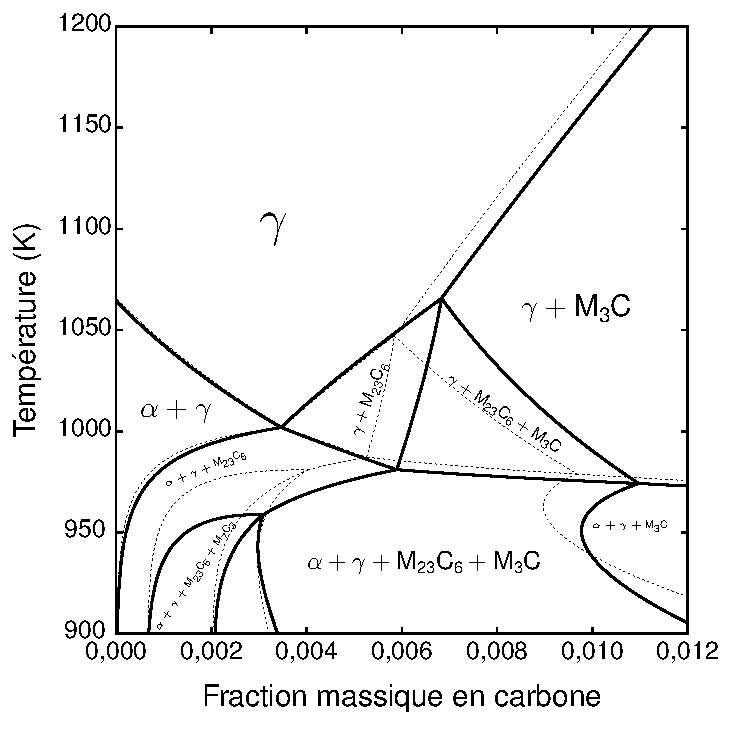
\includegraphics{figures/ch-02-diagram_pseudo_bin_aero}}
  }\hfill
  \subfloat[\label{fig:auto_pseudo_binaire}23MnCrMo5]{
    \centering\resizebox{0.48\textwidth}{!}{
      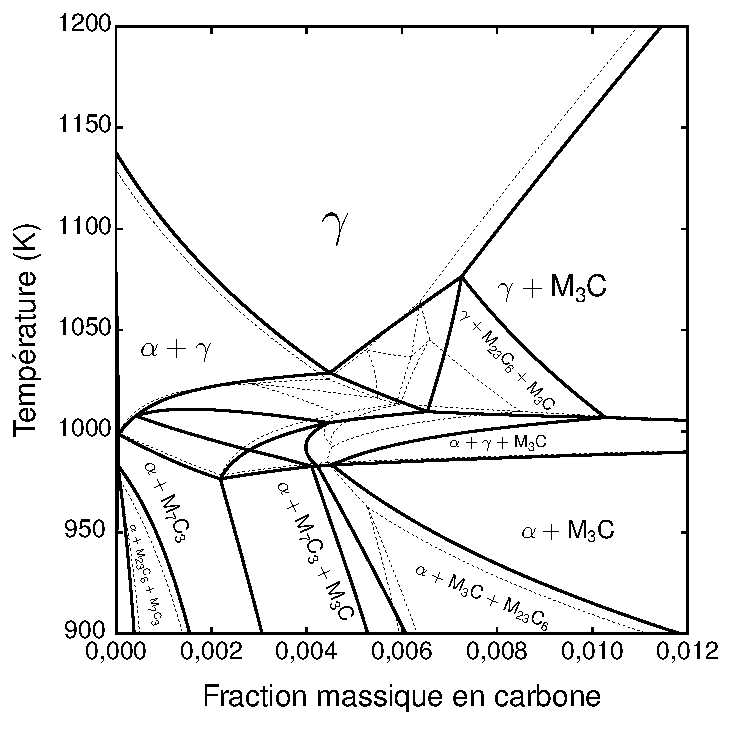
\includegraphics{figures/ch-02-diagram_pseudo_bin_auto}}
  }
  
  \caption{\label{fig:pseudo_binaires}Diagrammes pseudo-binaires établis en fonction de la fraction massique en carbone des alliages \protect\subref{fig:aero_pseudo_binaire} 16NiCrMo13 et \protect\subref{fig:auto_pseudo_binaire} 23MnCrMo5. Résultats obtenus avec Thermo-Calc~\cite{Andersson2002,Borgenstam2000}. Traits pleins base de données SSOL4, pontillés TCFE7.}
\end{figure}

Pour les deux nuances, la fraction massique en carbone permettant d'atteindre la saturation en surface dans la plage allant de \SIrange{1143}{1213}{\kelvin} se situe entre 0,009 et 0,011 et varie linéairement.  Les deux diagrammes de la Figure~\ref{fig:pseudo_binaires} montrent une réduction de la fraction massique en carbone pour la transformation de décomposition de l'austénite \textendash{} le point équivalent à la transformation eutéctoïde dans le système \ch{Fe-C} \textendash{} ce qui résulte de l'augmentation de l'activité de cet élément en présence des éléments d'alliage: la précipitation des carbures est favorisée. Dans tous les cas, en ce qui concerne l'enrichissement en carbone, les diagrammes montrent une limite de solubilité en carbone assez proche et les réponses en enrichissement aux conditions de cémentation et de carbonitruration au-delà de \SI{1150}{\kelvin} doivent rester similaires. Lors du revenu, les précipitations de cémentite alliée \ch{M3C} et de carbures \ch{M23C6} sont attendues pour des fractions massiques en carbone allant de 0,003 à 0,006, teneurs typiquement recherchées dans les couches traitées.

Des coupes pseudo-binaires établies en fonction de la fraction massique en azote sont tracées Figure~\ref{fig:pseudo_binaires_azote}. Ces diagrammes ne présentent plus de grandes similitudes avec leurs équivalents dans le système \ch{Fe-N}. Cela est dû a la présente d'éléments nitrurigènes, notamment le chrome, qui conduisent à la formation de nitrures \ch{MN} dans la plage de composition considérée. Pour des faibles teneurs en azote ($w_{N}\le 0,002$) le carbure prépondérant à basse température dans chaque alliage \textendash{} \ch{M23C6} pour la nuance 16NiCrMo13 et \ch{M7C3} pour 23MnCrMo5 \textendash{} se trouve à l'équilibre avec le nitrure \ch{MN}. En augmentant la teneur en azote, on observe simultanément la diminution de la température de transformation austénitique et le remplacement de ces carbures par la cémentite alliée. La phase \ch{Si3N4} est possible selon la base de données TCFE7. Cette phase ne sera pas considérée en raison de sa lente cinétique de précipitation à faible teneur en \ch{Si} dans les alliages \textendash{} cette phase est typiquement observée dans les aciers au silicium où la fraction en \ch{Si} dépasse 0,015.

\begin{figure}[!ht]
  \centering
  \subfloat[\label{fig:aero_pseudo_binaire_azote}16NiCrMo13]{
    \centering\resizebox{0.48\textwidth}{!}{
      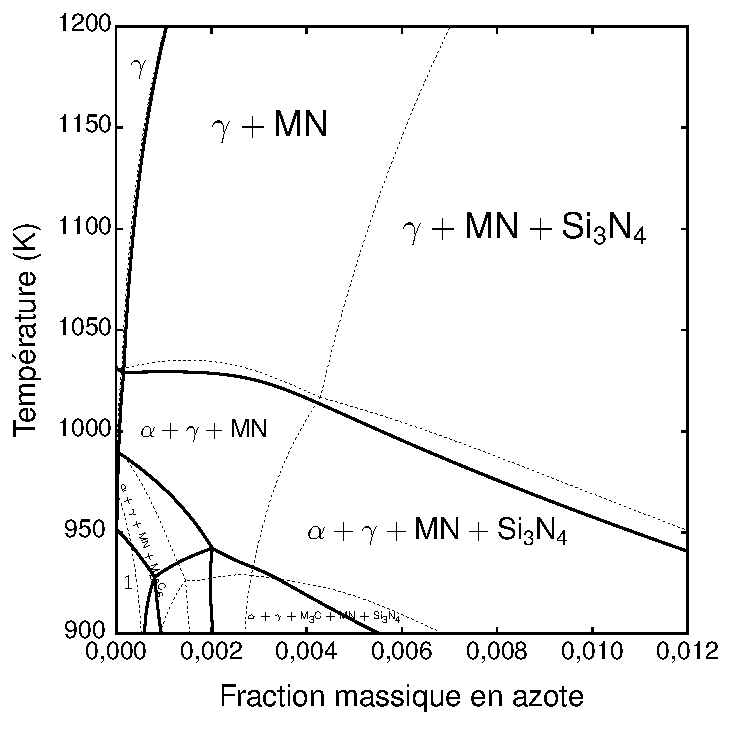
\includegraphics{figures/ch-02-diagram_pseudo_bin_aero_nitro}}
  }\hfill
  \subfloat[\label{fig:auto_pseudo_binaire_azote}23MnCrMo5]{
    \centering\resizebox{0.48\textwidth}{!}{
      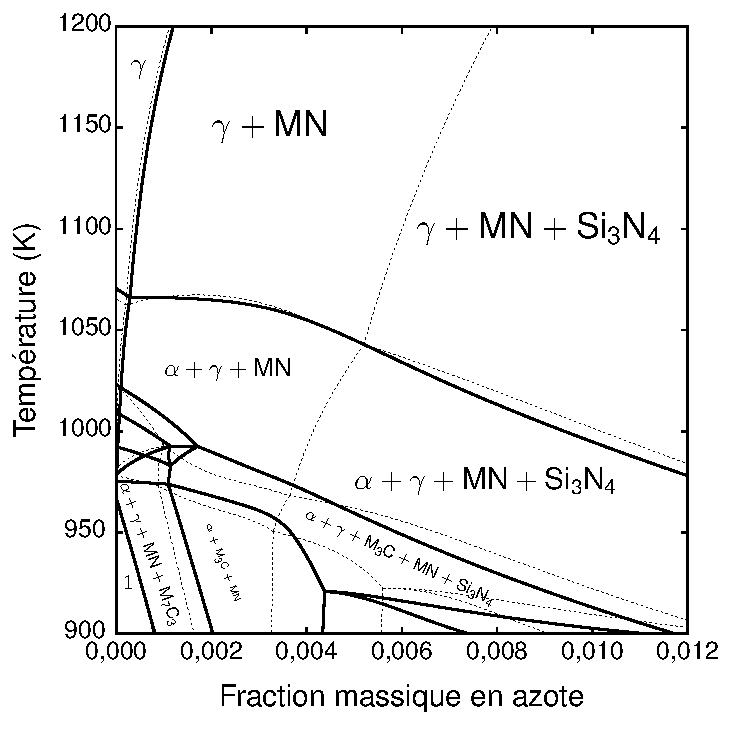
\includegraphics{figures/ch-02-diagram_pseudo_bin_auto_nitro}}
  }

  \caption{\label{fig:pseudo_binaires_azote}Diagrammes pseudo-binaires  établis en fonction de la fraction massique en azote des alliages \protect\subref{fig:aero_pseudo_binaire_azote} 16NiCrMo13 et \protect\subref{fig:auto_pseudo_binaire_azote} 23MnCrMo5. Résultats obtenus avec  Thermo-Calc~\cite{Andersson2002,Borgenstam2000}. Traits pleins base de données SSOL4, pontillés TCFE7.}
\end{figure}

\subsection{Coupes isothermes}

Bien que les diagrammes pseudo-binaires soient utiles à prédire les phases formées lors de la saturation et le comportement d'alliage pendant le refroidissement, des coupes isothermes peuvent être aussi utilisées pour le contrôle des procédés pendant la phase d'enrichissement. La Figure~\ref{fig:isothermes} présente des diagrammes établis en fonction des fractions en carbone et azote simulés à \SI{1173}{\kelvin} pour les deux alliages de cette étude. La limite de solubilité en azote \textendash{} une fraction massique inférieure à 0,001, à partir de laquelle des nitrures substitués de st{\oe}chiométrie \ch{MN} sont précipités \textendash{} s'avère être très peu dépendante de la fraction massique en carbone, lequel sature l'austénite autour de 0,01. La saturation en carbone conduit, pour les deux nuances, à la formation de cémentite alliée dans la région \og{}1\fg{}, des diagrammes, comme cela se voit également dans la Figure~\ref{fig:pseudo_binaires}. Les régions \og{}2\fg{} et \og{}3\fg{} ne présentent aucun intérêt dans le cas présent.

\begin{figure}[!bh]
  \centering
  \subfloat[\label{fig:isothermal_aero}16NiCrMo13]{
    \centering\resizebox{0.48\textwidth}{!}{
      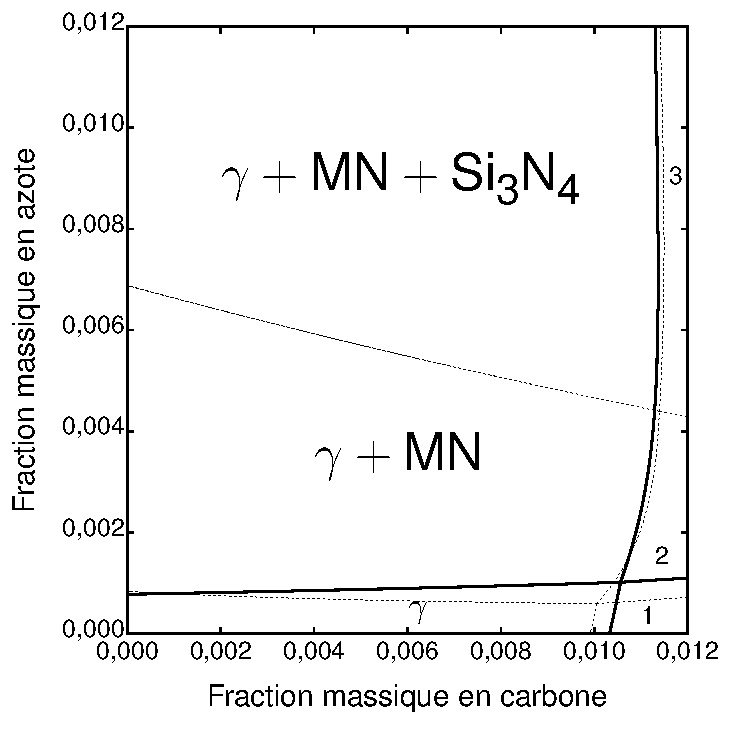
\includegraphics{figures/ch-02-diagram_isothermal_aero}}
  }\hfill
  \subfloat[\label{fig:isothermal_auto}23MnCrMo5]{
    \centering\resizebox{0.48\textwidth}{!}{
      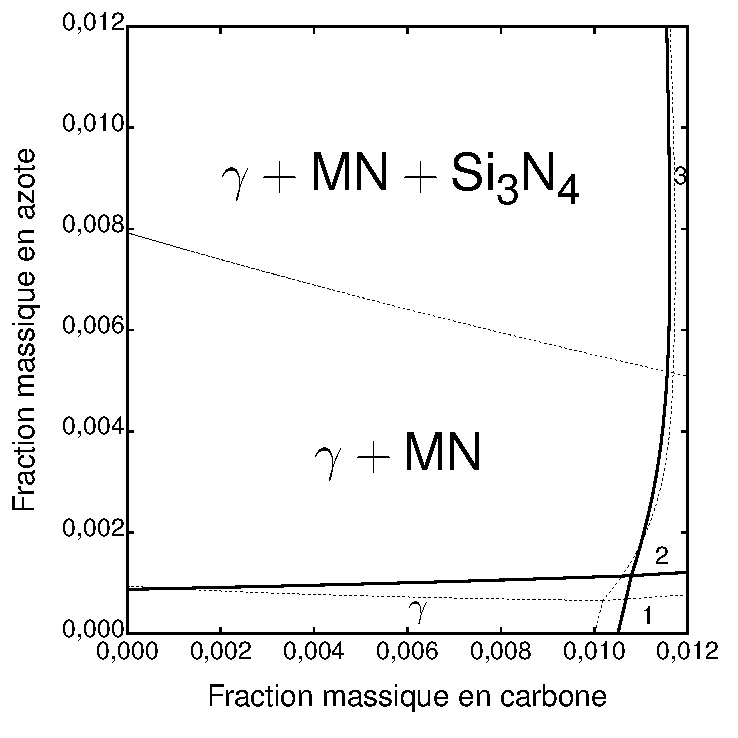
\includegraphics{figures/ch-02-diagram_isothermal_auto}}
  }

  \caption{\label{fig:isothermes}Coupes isothermes à \SI{1173}{\kelvin} établies en fonction des fractions massiques en carbone et azote des alliages \protect\subref{fig:isothermal_aero} 16NiCrMo13 et \protect\subref{fig:isothermal_auto} 23MnCrMo5. Résultats obtenus avec Thermo-Calc~\cite{Andersson2002,Borgenstam2000}. Traits pleins base de données SSOL4, pontillés TCFE7.}
\end{figure}

Comme lors des phases de cémentation, la condition à la limite pour le carbone correspond à une saturation en carbone de la surface dans l'austénite, la précipitation de cémentite n'est donc pas prise en compte \textemdash{} on suppose que la formation et solution de \ch{M3C} est instantanée et la phase n'est pas utilisée dans la simulation. Cela rend possible de réaliser la simulation sans adopter un modèle d'homogénéisation et donc plus rapidement. En revanche, les fractions massiques en azote visées au-delà de 0,003, introduites dans les alliages par la carbonitruration et la nitruration austénitique, impliquent la précipitation de nitrures du type \ch{MN} et un appauvrissement en éléments d'alliage, notamment le chrome et le molybdène, de la matrice austénitique.  Pour tenir compte de cette précipitation et de ses effets, il faut recourir à la Figure~\ref{fig:consommation_matrice} qui montre la consommation du chrome conduisant à la formation des nitrures \ch{MN}. On observe l'évolution de l'azote en solution solide en fonction de la teneur totale dans l'alliage. Jusqu'à la limite de solubilité, la pente des courbes de la Figure~\ref{fig:consommation_azote} est unitaire. Ensuite, les courbes suivent un chemin qui dépend de la composition de l'alliage. Des résultats similaires sont obtenus avec les bases de données TCFE7 et SSOL4. Comme les matériaux sont traités pendant une durée suffisamment longue pour supposer un équilibre des phases, l'azote ainsi calculé sera considéré comme étant représentatif de la composition de la martensite.% obtenue lors de la trempe.

\begin{figure}[h]
  \centering
  \subfloat[\label{fig:consommation_chrome}Chrome en solution solide.]{
    \centering\resizebox{0.48\textwidth}{!}{
    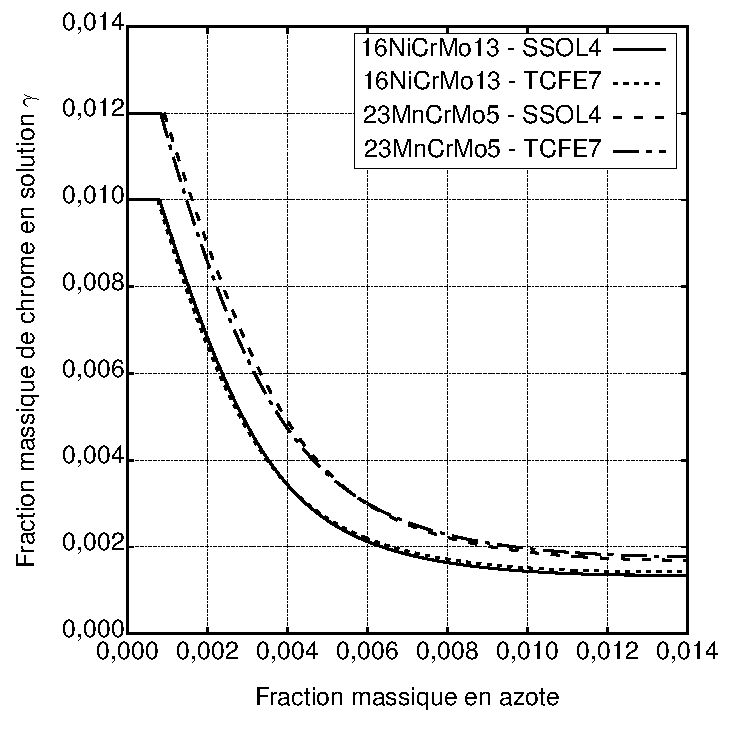
\includegraphics{figures/ch-02-consommation_alliage}}
  }\hfill\subfloat[\label{fig:consommation_azote}Azote en solution solide.]{
    \centering\resizebox{0.48\textwidth}{!}{
    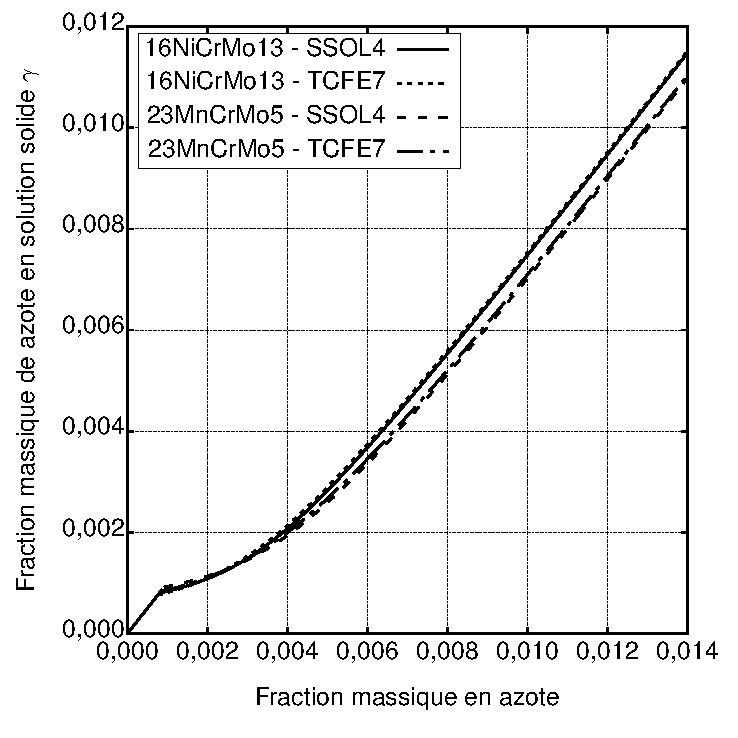
\includegraphics{figures/ch-02-consommation_azote}}
  }

  \caption{\label{fig:consommation_matrice}Simulation de la consommation des éléments en solution solide et formation de nitrures à \SI{1173}{\kelvin}. Résultats obtenus avec Thermo-Calc~\cite{Andersson2002,Borgenstam2000}, bases de données SSOL4 et TCFE7.}
\end{figure}

Les principales caractéristiques des alliages étudiés à retenir, établies au cours de la Section~\ref{sec:studied_alloys} à l'aide de Thermo-Calc~\cite{Andersson2002,Borgenstam2000}, peuvent être résumées ainsi:
\begin{itemize}
  \item les seuils de précipitation de cémentite en domaine $\gamma$ à \SI{1173}{\kelvin} correspondent à des fractions massiques de l'ordre de 0,01. Cependant, l'activité associée à cette valeur \textendash{} en utilisant le graphite comme état de référence \textendash{} n'est pas la même pour les deux nuances. Pour les simulations d'enrichissement, la valeur simulée pour chaque nuance doit être utilisée comme condition à la limite si l'on désire considérer une condition de précipitation de \ch{Fe3C} en surface;
  \item on s'attend à la formation de nitrures du type \ch{MN} pendant l'enrichissement en azote, ce qui doit advenir pour des fractions massiques de cet élément de l'ordre de 0,001. Cette précipitation produit un appauvrissement de la matrice de l'alliage que doit favoriser un comportement au revenu plus proche de celui du système \ch{Fe-C-N}. 
\end{itemize}

\section{Métallurgie de la carbonitruration}
\label{sec:metallurgie_cn}

Les sections précédentes ont principalement abordé le cas de l'équilibre des systèmes métallurgiques étudiés et donc précisent les phases formées pendant l'enrichissement en carbone et en azote. Cette étape est nécessaire pour le contrôle des procédés thermochimiques car elle sert à connaître les seuils de précipitation des nitrures et des carbures, ainsi que l'appauvrissement en éléments d'alliage dans les matrices enrichies. Maintenant, il convient de discuter du comportement des alliages au cours des étapes conférant les propriétés finales à partir des compostions établies par l'enrichissement. La martensite au carbone et à l'azote sera d'abord traitée avant que soient abordées les réponses au revenu des aciers faiblement alliés contenant ces éléments interstitiels.

\subsection{La martensite au carbone et à l'azote}
\label{sec:martensite_cn}

L'obtention des propriétés mécaniques désirées après les traitements thermochimiques dans le domaine austénitique résulte généralement d'une séquence de trempe et revenu. Cela implique une transformation de type martensitique pendant la trempe~\cite{Steel2006}, qui par contraction thermique, dépasse le seuil de contraintes requis pour former la martensite~\cite{Khachaturyan1983}. L'approche mécanique de ce genre de transformation est décrite dans une publication classique de \citet{Kurdjumov1976}. Beaucoup de travaux sont disponibles dans la littérature sur la martensite au carbone des aciers faiblement alliés et sur ses transformations pendant le revenu. Un travail de référence de \citet{Krauss1999} compile de manière concise les propriétés et structures attendues dans des situations rencontrées dans les traitements thermochimiques.

Si l'on considère les enrichissements en carbone dans la plage de 0,005-0,006 en fractions massiques, on doit s'attendre à observer la formation d'une microstructure martensitique en lattes pour des taux de refroidissement typiques~\cite{Krauss1999}. Cette morphologie n'est pas seulement dépendante de la composition \textendash{} ponctuelle dans les traitements thermochimiques \textendash{} et donc de la température $M_{s}$ de début de transformation martensitique, mais aussi de la température à laquelle la transformation s'est passée, laquelle peut être influencée par le milieu de trempe~\cite{Umemoto1983}. Du fait de son caractère fragile, cette martensite est normalement soumise au revenu avant l'utilisation des pièces trempées. Le revenu de la martensite au carbone peut être appréhendé à partir de la plage de température et du traitement thermique appliqué. De manière plus générale, il intègre l'histoire thermique de la pièce après la réalisation de la trempe et donc comprend même les transformations issues des étapes du traitement cryogénique ainsi que le vieillissement à la température ambiante. Dans ce contexte, \citet{Cheng1988} décrivent la suite de transformations qui ont lieu dans la martensite \ch{Fe-C}, suite qui est affectée par la présence d'éléments d'alliage dont l'effet principal est de décaler la plage des températures de chaque régime, notamment en ce qui concerne la transformation des carbures intermédiaires. \citet{Morra2001} fournissent données des cinétiques de ces processus pour quelques aciers.

Dans le cas de la martensite à l'azote, un nombre très limité de publications est disponible~\cite{Catteau2014,Catteau2016}. La littérature est centrée sur le système \ch{Fe-N}, pour lequel les transformations métallurgiques induites par les étapes de revenu et de vieillissement à la température ambiante sont connues~\cite{Kaplow1983,vanGent1985,Mittemeijer1988,Cheng199013,Cheng19902857,Fall1996,vanGenderen1997,Sherby2008}. La formation du nitrure intermédiaire \ch{Fe16N2} a lieu à température ambiante après une centaine d'heures de vieillissement, ce qui apporte une augmentation de la résistance mécanique de la martensite \ch{Fe-N}. Avec le revenu, ce nitrure cohérent devient incohérent et donc la résistance supplémentaire qu'il apporte n'est pas conservée. Bien que comportement, \emph{i.e.} dureté, après trempe de la martensite au carbone puisse être directement décrit par la teneur interstitielle~\cite{Cohen1968,Norstrom1976,Krauss1999,Hutchinson20115845}, le rôle de l'azote n'est pas explicité. 

Pour des faibles teneurs en azote, \citet{Briant1982} montre que cet élément peut induire une fragilisation pendant le revenu. De plus, pour les aciers faiblement alliés, en raison de la formation de nitrures à la température d'enrichissement, la martensite obtenue diffère de la composition de l'alliage de départ, et est plus proche de celle du système \ch{Fe-N}. \citet{Cheng1992} comparent le revenu d'une martensite mixte au carbone et à l'azote (\ch{Fe-C-N}) à celui des systèmes binaires \ch{Fe-C} et \ch{Fe-N}. Les auteurs~\cite{Cheng1992} concluent que la présence simultanée des deux interstitiels accélère la décomposition \ch{Fe16N2 -> Fe4N} et retarde celles des carbures intermédiaires en cémentite et de l'austénite résiduelle, lesquels restent métastables à des températures plus élevées. L'azote en solution solide réduit également la vitesse critique de refroidissement pour la trempe \textendash{} augmentation de la trempabilité de l'alliage. Néanmoins, l'austénite résiduelle est une réalité dans les aciers et sa transformation finale en martensite n'est normalement pas complète~\cite{Steel2006}.

\citet{Norstrom1976} a proposé un modèle pour prédire la limite élastique de la martensite en fonction de sa morphologie et de sa teneur en carbone (Équation~\ref{eq:norstrom_model}). Cette équation prend en compte la friction interne dans le fer pur $\sigma_{0}$, la contribution des éléments d'alliage $\sigma_{1}$, deux termes de Hall-Petch pour incorporer les tailles $d$ des lattes et $D$ des paquets de martensite, la densité intrinsèque de dislocations dans le fer pur martensitique $\rho_{0}$ et son augmentation avec la teneur en carbone $K(C)$.

\begin{equation}
  \sigma_{y}=\sigma_{0}+\sigma_{1}+\frac{k_{y}}{D^{\nicefrac{1}{2}}}
    +\frac{k_{s}}{d^{\nicefrac{1}{2}}}+
    \alpha{Gb}\biggr[\rho_{0}+K(C)\biggr]^{\nicefrac{1}{2}}
  \label{eq:norstrom_model}
\end{equation}

La dépendance du dernier terme de l'Équation~\ref{eq:norstrom_model} avec la racine carrée de la densité de dislocations avait déjà été proposée par \citet{Cohen1968} et trouve ses bases physiques dans la mécanique des dislocations~\cite{Haasen19962009,Hutchinson20115845}. Comme la densité des dislocations augmente de manière linéaire avec la teneur en carbone~\cite{Krauss1999,Morito20031475}, on peut vérifier la validité de cette approche en traçant la résistance mécanique en fonction de la racine carrée de la teneur en interstitiels. Ce modèle reste applicable jusqu'à la transformation de la martensite cubique en martensite quadratique connue sous l'appellation \og{} point-H \fg{}~\cite{Sherby2008}. 
Selon \citet{vanGent1985} la teneur limite en azote pour la transformation de la martensite de cubique à quadratique se situe à une fraction massique d'environ 0,002. Cette valeur n'est pas en accord avec celle rapportée par \citet{Sherby2008} qui la situent à une fraction atomique de 0,0275 pour le carbone et pour l'azote. L'utilisation des fractions atomiques semble plus raisonnable dans ce cas étant donné le caractère du phénomène physique mis en jeu: l'occupation des sites interstitiels produisant une déformation quadratique du réseau cristallin. Cette valeur en fraction atomique correspond à une fraction massique en carbone de 0,006 et en azote de 0,0075.

Bien que $\sigma_{y}$ dépende de plusieurs facteurs comme la morphologie de la martensite, le durcissement par solution solide et la densité et la mobilité des dislocations~\cite{Krauss1999}, la dépendance la plus marquée est celle relative à la teneur en interstitiels en solution solide. Cela permet une comparaison directe entre les matériaux de base fer~\cite{Grange1977,Hutchinson20115845}. \citet{Hutchinson20115845} montrent, par exemple, que pour les nuances~\footnote{Ici rapportées en pourcentages massiques.} Fe-1,7Mn-0,23Si-0,12C et Fe-1,7Mn-0,21Cr-0,23Si-0,23C la contribution des éléments d'alliage dans l'Équation~\ref{eq:norstrom_model} correspond à 10-12\% de la limite élastique, alors que la contribution due à la taille de grain est à environ 13\%, les dislocations à 12-13\%, la structure martensitique à 35-39\% et la contribution de la teneur en interstitiels en solution solide à 61-66\%.

\subsection{Réponses des couches carbonitrurées}
\label{sec:carbonitrurationalliages}

% \cite{Xiong2013} \cite{Xiong2008}

Dans un second temps, il convient de présenter quelques résultats importants relatifs aux traitements thermochimiques des aciers faiblement alliés. Les principaux aspects spécifiques dont ce paragraphe fera état sont \begin{inparaenum}[(i)] \item la dureté après revenu, \item la fraction en austénite résiduelle et \item les précipités formés lors du revenu. \end{inparaenum} Les alliages comparés sont présentés sur le Tableau~\ref{tab:comparaison_alliages}.

\begin{table}[!hb]
  \caption{\label{tab:comparaison_alliages}Comparaison entre les compositions nominales  en pourcentage massique des alliages cités dans la Section~\ref{sec:carbonitrurationalliages} et les alliages étudiés.}
  
  \centering{}\footnotesize{}%
  \begin{tabular}{\$c^c^c^c^c^c^c^c^c}
    \toprule[2pt] 
    \rowstyle{\bfseries}
    Alliage & Fe & C & Si & Mn & Cr & Ni & Mo & Autre(s)
    \tabularnewline
    \midrule[2pt]
    15NiMoCr10~\cite{Loukachenko2006} 
    & bal. & 0,15 & 1,19 & 0,44 & 0,99 & 2,50 & 1,98 & V-0,29
    \tabularnewline[6pt]  
    27CrMo4~\cite{Loukachenko2006}
    & bal. & 0,27 & - & - & 1,15 & - & 0,27 & -
    \tabularnewline[6pt]
    27MnCr5~\cite{Loukachenko2006}
    & bal. & 0,27 & 0,25 & 1,20 & 0,98 & - & - & -
    \tabularnewline[6pt]
    Nuance 1~\cite{Preciado2006}
    & bal. & 0,18 & 0,25 & 0,75 & 1,00 & - & 0,20 & -
    \tabularnewline[6pt]
    Nuance 2~\cite{Preciado2006}
    & bal. & 0,14 & 0,25 & 0,45 & 0,95 & 3,25 & 0,25 & -
    \tabularnewline[6pt]
    Nuance B~\cite{Marray2012}
    & bal. & 0,18 & 0,19 & 0,34 & 3,12 & 0,40 & 0,46 & V-0,70 W-0,45
    \tabularnewline[6pt]    
    16NiCrMo13 & bal. & 0,16 & 0,25 & 0,45 & 1,00 & 3,20 & 0,25 & -
    \tabularnewline[6pt] 
    23MnCrMo5 & bal. & 0,23 & 0,25 & 1,30 & 1,20 & 0,10 & 0,25 & -
    \tabularnewline
    \bottomrule
  \end{tabular}
\end{table}

\subsubsection*{Dureté après revenu} 

L'introduction intentionnelle de silicium minimise la chute de dureté lors du revenu à \SI{573}{\kelvin} de l'acier 15NiMoCr10 cémenté~\cite{Loukachenko2006}. Cela résulte du fait que l'introduction de \ch{Si} retarde la cinétique de décomposition des carbures du type $\varepsilon-\ch{Fe_{2-4}C}$ formés durant le revenu en cémentite \ch{M3C}, la présence de ces carbures $\varepsilon$ étant confirmée par microscopie électronique à transmission. Ce n'est pas le cas pour les alliages 27CrMo4 et 27MnCr5 carbonitrurés, pour lesquels le revenu à cette température (\SI{573}{\kelvin}) produit une chute plus importante en dureté pour une même dureté initiale \textendash{} qui dépend presque uniquement de la teneur totale en éléments interstitiels en solution solide pour les aciers faiblement alliés~\cite{Grange1977}. \citet{Loukachenko2006} a utilisé ces alliages \textendash{} 27CrMo4 et 27MnCr5 \textendash{} dans le but de vérifier des résultats présentés dans la littérature sur l'alliage 20Cr4, résultats qui établissaient que le matériau conserve sa dureté \og{}de trempe\fg{} même après un revenu à \SI{573}{\kelvin} grâce à une précipitation secondaire de nitrures du type $\gamma^{\prime}-\ch{Fe4N}$. Ces résultats n'ont pas pu être reproduits, l'auteur~\cite{Loukachenko2006} ayant mis en évidence une décroissance continue de la dureté lors du revenu à \SI{573}{\kelvin}. En fait, même pour l'alliage 15NiMoCr10 cémenté, une certaine chute en dureté a été observée après le revenu \textendash{} quand on la compare à l'état après trempe \textendash{} ce qui a été attribué à la précipitation de carbures de type \ch{M23C6} et \ch{M6C}, le second étant lié à la teneur modérée en molybdène (une fraction massique d'environ 0,02) dans cette nuance, en bon accord avec des simulations réalisées à l'aide de Thermo-Calc~\cite{Andersson2002,Borgenstam2000}. 

On doit remarquer que l'alliage 23MnCrMo5 ici traité présente des similitudes chimiques avec la nuance 27MnCr5 \textemdash{} Tableau~\ref{tab:comparaison_alliages}. Plus spécifiquement, l'enrichissement en carbone et/ou en azote des alliages 23MnCrMo5 et 27MnCr5 peut conduire à la même composition en surface si la teneur en \ch{Mo} dans la seconde nuance \textendash{} où le molybdène n'est pas ajouté intentionnellement \textendash{} se trouve proche de celle de l'alliage 23MnCrMo5. Dans ce cas, on ne s'attend pas à ce que l'alliage  soit capable de retenir la dureté nécessaire si des contraintes de Hertz de l'ordre de \SI{2,45}{\giga\pascal} sont imposées après revenu à \SI{573}{\kelvin}, conditions visées par \citet{Loukachenko2006}.

\subsubsection*{Austénite résiduelle} 

Un autre aspect qui doit être considéré pour décrire comment s'établissent les propriétés mécaniques des aciers est la fraction d'austénite résiduelle obtenue après trempe. Cela résulte de la transformation incomplète de l'austénite dans les microstructures métastables à basse température pendant le refroidissement fortement hors équilibre~\cite{Steel2006}. L'effet de la présence d'austénite résiduelle est controversé dans la littérature~\cite{Preciado2006}: bien qu'elle puisse diminuer la résistance à l'usure ou la fatigue de contact, cette phase hors équilibre promeut la fermeture des fissures produites par fatigue et donc diminue leur vitesse de propagation.

\citet{Loukachenko2006} montre, par exemple, que la fraction volumique $V_{\gamma_{R}}$ d'austénite résiduelle $\gamma_{R}$ pour la nuance 15NiMoCr10 en fonction de la température du milieu de trempe $T_{q}$ est en bon accord avec l'Équation~\ref{eq:koistinen} proposée par \citet{Koistinen1959}. Dans ce cas, le traitement cryogénique est considéré comme une continuation directe de la trempe. Après revenu, l'austénite résiduelle n'est plus observée du fait de sa décomposition en martensite. \citet{Yahia1995} montre à partir d'une étude bibliographique et expérimentale la validité de l'approche de \citet{Koistinen1959} pour l'effet de l'azote dissous dans l'austénite à partir du calcul de la température initiale de formation de la martensite $M_{s}$.

\begin{equation}
  V_{\gamma_{R}}=100\times\exp[-0,011(M_{s}-T_{q})]
  \label{eq:koistinen}
\end{equation}

L'effet d'un traitement cryogénique après cémentation et revenu des alliages notés \og{}Nuance 1\fg{} et \og{}Nuance 2\fg{} dans le Tableau~\ref{tab:comparaison_alliages} est étudié par \citet{Preciado2006}, contrairement à la pratique habituelle consistant à réaliser ce traitement avant le revenu. Il faut remarquer que la composition moyenne de la \og{}Nuance 2\fg{} rapportée par les auteurs~\cite{Preciado2006} est équivalente à celle de l'alliage 16NiCrMo13. Ce traitement cryogénique réalisé après revenu a amélioré la résistance à l'usure des alliages étudiés, ce qui a été attribué à la ségrégation du carbone et des éléments d'alliage induite par le cycle cryogénique. Cependant, la mise en évidence de ce mécanisme n'a pas été établie.

\subsubsection*{Précipités observés expérimentalement}

\citet{Yahia1995} met en évidence après trempe la formation de précipités polyédriques avec des dimensions de l'ordre de \SI{0,5}{\micro\metre} aux anciens joints de grains austénitiques de l'alliage 27CrMo4. La formation de précipités sous forme de bâtonnets avec des longueurs de l'ordre de \SI{0,1}{\micro\metre} et sous forme de polyèdres avec une longue diagonale de l'ordre de \SI{0,2}{\micro\metre} a aussi été mise en évidence. L'identification de ces précipités par microscopie électronique en transmission (MET) montre que les bâtonnets sont des nitrures \ch{CrN} (hors contour de grain), tandis que les précipités sous forme de polyèdre sont des carbures du type \ch{M3C} contenant \ch{Fe}, \ch{Mn} et \ch{Cr}. Dans le cas de la nuance 27MnCr5, une faible densité de précipités le long des contours de grain austénitiques a été observée pour la cémentation et la carbonitruration à des teneurs massiques en carbone supérieures à 0,65\%, contrairement à l'alliage 27CrMo4. Ces effets n'ont pas été mis en évidence après nitruration. Grâce à des analyses par micro-sonde électronique et diffraction des rayons x, ces précipités ont aussi été identifiés comme étant des carbures de type \ch{M3C}. Ces résultats~\cite{Yahia1995,Loukachenko2006} concernant l'alliage 27CrMo4 seront confrontés dans ce mémoire avec ceux obtenus pour la nuance 16NiCrMo13. Une attention particulière sera prêtée à l'estimation des niveaux d'austénite résiduelle après trempe, compte tenu du fait que la principale différence entre les alliages étudiés réside dans leurs teneurs en nickel respectives.

\citet{Marray2014} observent la présence de carbures \ch{M23C6} et \ch{M7C3} après enrichissement de l'alliage noté \og{}Nuance B\fg{}, alors qu'aucune précipitation à haute température n'est observée pour la nuance 16MnCr5, laquelle est aussi assez proche de la nuance 23MnCrMo5. Cette observation est en accord avec les diagrammes des Figures~\ref{fig:auto_pseudo_binaire}~et~\ref{fig:auto_pseudo_binaire_azote}. De plus, la séquence de précipitation observée tout au long du profil enrichi pour la \og{}Nuance B\fg{} est en accord avec ce à quoi l'on doit s'attendre selon des simulations réalisées à l'aide de Thermo-Calc~\cite{Andersson2002,Borgenstam2000}, ce qui montre la fiabilité de l'approche CALPHAD pour les étapes d'enrichissement. Enfin, \citet{Marray2012} compile des expressions utiles pour le calcul des températures de début de transformation martensitique.

\clearpage\section{Conclusion}

Dans le Chapitre~\ref{ch:thermodynamique} nous avons introduit les concepts de la métallurgie à l'équilibre et hors équilibre pour les systèmes modèles à base fer et faiblement alliés. La simulation des diagrammes pseudo-binaires et isothermes des nuances industrielles étudiées a été réalisée, simulation dont on se servira au Chapitre~\ref{ch:reponse_metallurgique}. Les principaux points du chapitre peuvent être résumés ainsi:
\begin{itemize}
  \item l'approche CALPHAD permet l'estimation des phases à l'équilibre pour un ensemble de conditions et de compositions données en fonction de la disponibilité des données thermodynamiques. L'obtention de ces données est normalement empirique et même si des efforts sont réalisés pour diminuer ce besoin avec l'emploi des méthodes \textit{ab initio}, reste que CALPHAD est semi-empirique;
  
  \item les principales phases à l'équilibre composant les systèmes à base de fer, carbone et azote sont la ferrite, l'austénite, \ch{M3C}, \ch{Fe4N_{(1-x)}} et \ch{Fe2N_{(1-x)}}. L'inclusion d'éléments carburigènes et nitrurigènes conduit à la formation des carbures et des nitrures \ch{M23C6}, \ch{M7C3}, \ch{MN}, \ch{MnSiN2}, etc.;
  
  \item en présence d'éléments carburigènes, l'allure à haute température (domaine  $\gamma$) des diagrammes pseudo--binaires établis en fonction du carbone dans les alliages étudiés reste proche de celle du système \ch{Fe-C}, alors que le carbure en équilibre dans cette région reste le même \ch{M3C}. Ce n'est pas le cas pour les pseudo--binaires établis en fonction de l'azote où le nitrure \ch{MN} remplace \ch{Fe2N_{(1-x)}}. Selon les simulations réalisées, en diminuant la température, le carbure dont on favorise la précipitation après enrichissement en carbone est le \ch{M23C6} pour l'alliage 16NiCrMo13 et le \ch{M7C3} pour la nuance 23MnCrMo5;
  
  \item l'approche thermodynamique est limitée par le fait que les traitements de cémentation et de carbonitruration sont terminés par une trempe. Par conséquent sa validité reste limitée à la seule phase d'enrichissement. Cependant, les simulations des diagrammes de phase peuvent aider à identifier les carbures et nitrures probables formés lors du revenu.
\end{itemize}

\endinput
  \part{Résultats expérimentaux}
  \label{part:part_2}
  \cleardoublepage\chapter{Dynamique des traitements}
\label{ch:caracterisation_atmospheres}

\vfill

Pour suivre la structure adoptée dans la Partie~\ref{part:part_1}, les résultats expérimentaux concernant la mise au point des procédés seront présentés dans ce chapitre avant les réponses métallurgiques des alliages exposées Chapitre~\ref{ch:reponse_metallurgique}. La Section~\ref{sec:experimental_system} présente les dispositifs expérimentaux employés pour les traitements thermochimiques et les études des atmosphères. Ensuite, la caractérisation du réacteur et la méthode d'analyse à basse pression sont présentées Section~\ref{sec:caracterization_gaz}. Le comportement hydrodynamique du réacteur est caractérisé dans le but de mieux maîtriser les conditions aux limites des traitements thermochimiques. Cela se fait initialement à partir de la connaissance de la fonction de distribution du temps de séjour. L'allure et les temps caractéristiques de cette distribution déterminent, pour un ensemble de conditions d'opération données, le type de couplage entre l'hydrodynamique et la cinétique réactionnelle des gaz employés pour les traitements. Ensuite, on présente le système de prélèvement du chromatographe à basse pression. La mise au point de l'atmosphère carburante à base de mélanges \ch{CO-H2} est présentée dans la Section~\ref{sec:classical_carburizing}, qui présente les calculs de température de point de rosée pour les alliages choisis.  Des études sur la pyrolyse de l'acétylène ainsi que sur la cémentation à partir d'hydrocarbures font partie de la Section~\ref{sec:pyrolyse_acetylene}.  La cinétique de cémentation, \textit{i.e.} la prise de masse en fonction du temps, est étudiée à l'aide d'une thermobalance couplée au réacteur. En ce qui concerne la nitruration à partir de l'ammoniac, la Section~\ref{sec:pyrolyse_ammonia} présente son comportement de décomposition de \ch{NH3} et la cinétique de décarburation pendant l'étape de nitruration. Ces résultats sont utilisés pour réaliser les traitements des alliages qui seront analysés d'un point de vue métallurgique au Chapitre~\ref{ch:reponse_metallurgique} et confrontés aux simulations de décomposition des précurseurs au cours des traitements au Chapitre~\ref{ch:modelisation_cinetique}.

\vfill\newpage

\section{Système expérimental}
\label{sec:experimental_system}

\begin{figure}[!b]
  \subfloat[\label{fig:reacteur_pa}Réacteur à la pression atmosphérique.]{
     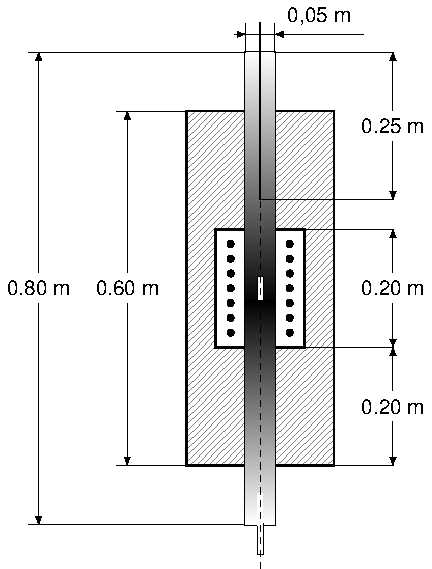
\includegraphics[width=6.5cm]{figures/ch-03-reacteur_pa}
  }\hfill
  \subfloat[\label{fig:reacteur_bp}Réacteur à basse pression.]{
    \raisebox{20mm}{
      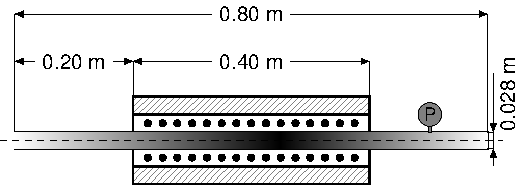
\includegraphics[width=8.5cm]{figures/ch-03-reacteur_bp}}
  }

  \caption{\label{fig:experimental_system}Schémas des réacteurs employés pour les traitements thermochimiques et le suivi de la décomposition des précurseurs.}
\end{figure}

\subsection{Réacteur à la pression atmosphérique}
\label{sec:reacteur_pa}

Les études de traitements thermochimiques ont été réalisées dans un réacteur tubulaire en alumine présentant un rapport surface-volume $\nicefrac{S}{V}=\SI{0,8}{\per\centi\metre}$ et un diamètre de \SI{50}{\milli\metre} schématisé Figure~\ref{fig:reacteur_pa}. L'enceinte de traitement en \ch{Al2O3} est considérée inerte, \textit{i.e.} les transformations chimiques des gaz précurseurs sont produites uniquement en phase homogène ou sur les surfaces des pièces traitées.  Pour assurer l'homogénéité en composition des gaz utilisés pour les traitements thermochimiques, un système d'alimentation de gaz permet le mélange des précurseurs dans un volume de ballast d'environ \SI{1000}{\cubic\centi\metre} avant introduction dans la zone de traitement du réacteur. L'injection des gaz se fait par un tuyau en alumine d'un diamètre interne de \SI{2}{\milli\metre} entrant par la partie supérieure du réacteur et injectant les gaz à \SI{100}{\milli\metre} de la partie supérieure de l'échantillon. Ceci permet d'assurer, pour les débits typiquement utilisés dans ce réacteur, de l'ordre de \SIrange{500}{1000}{\sccm}, la dissipation du jet de gaz produit par l'injecteur et un écoulement laminaire autour de la pièce traitée. Le chauffage est assuré par des résistances électriques placées autour de la zone centrale du tube réacteur sur une longueur de \SI{0,2}{\metre}, produisant une région de température constante d'environ \SI{80}{\milli\metre} et permettant des cycles thermiques jusqu'à \SI{1373}{\kelvin}. Cette zone est représentée sur la Figure~\ref{fig:experimental_system} par un gradient de gris, le rectangle central représentant la position de l'échantillon. Compte tenu de la longueur de cette région, pour assurer un traitement homogène des pièces, les échantillons ne doivent pas dépasser environ \SI{50}{\milli\metre} dans la direction de l'axe du réacteur. Par conséquent, des échantillons ayant des dimensions de \SI{40 x 14 x 4} {\milli\metre} ont été découpés dans des barres forgées des deux matériaux étudiés et polis au papier abrasif jusqu'à une granulométrie de \SI{14}{\micro\metre} avant traitement. Pour les suivis de prise de masse avec la thermobalance, chaque échantillon de longueur \SI{40}{\milli\metre} a été découpé en deux en raison de la limite de masse imposée par la thermobalance, conduisant à des pièces ayant pour dimensions \SI{20 x 14 x 4}{\milli\metre}. 

La caractérisation des produits à la sortie du réacteur est faite par un équipement de chromatographie gazeuse Carlo Erba Instruments modèle GC6000 Vega Series 2. Le système de chromatographie est équipé d'un détecteur à ionisation par flamme et d'un autre par conductivité thermique (Annexe~\ref{an:caracterisation_atmospheres}). La thermobalance couplée au système n'est pas représentée et se trouve à la verticale du réacteur. Une description détaillée de la thermobalance employée ici et de la technique de thermogravimétrie est fournie par \citet{Jaoul2004}. Un hygromètre Dewpro MMY 245 est aussi disponible pour la mesure de la température du point de rosée des atmosphères de cémentation.

\subsection{Réacteur à basse pression}
\label{sec:reacteur_bp}

\begin{figure}[!b]
  \centering\resizebox{0.6\textwidth}{!}{
    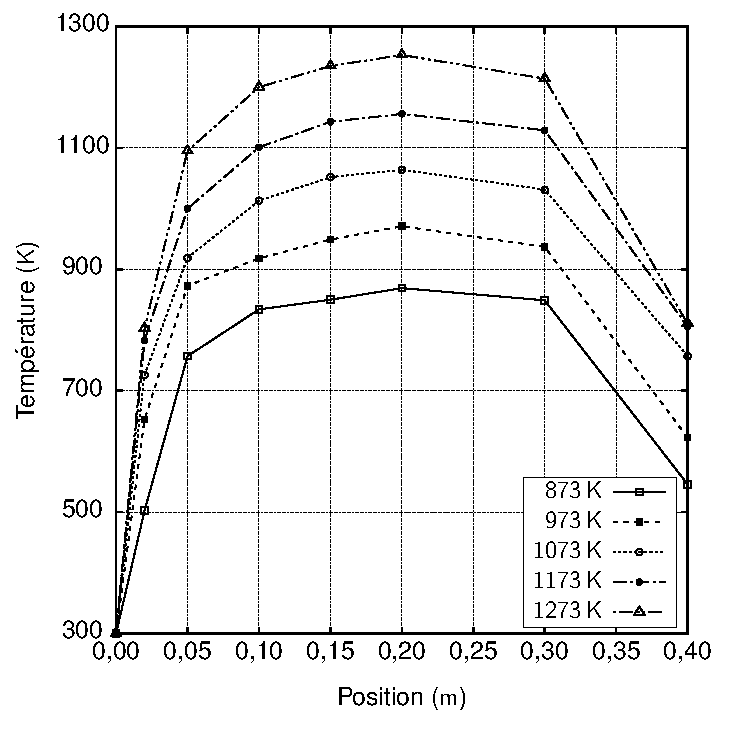
\includegraphics{figures/ch-03-reactor_bp_temperature}}
  
  \caption{\label{fig:temperature_profiles_bp}Profils de température dans la zone chaude du réacteur dans les expériences à basse pression (Figure~\ref{fig:reacteur_bp}) en fonction de la coordonnée de l'axe du réacteur mesurée à partir de l'entrée dans la zone de contrôle pour des températures de consigne entre \SIrange{873}{1273}{\kelvin}.}
\end{figure} 

Le système employé pour les études à basse pression est assez similaire de celui employé à la pression atmosphérique et le contrôle de son alimentation est réalisé par le même système et donc le même volume de ballast pour assurer l'homogénéité des gaz à l'entrée. L'alimentation des gaz est faite par la gauche (Figure~\ref{fig:reacteur_bp}), les systèmes de mesure de pression, de pompage et de caractérisation étant placés à droite. Le contrôle de température est opéré sur une longueur de \SI{0,4}{\metre} par des résistances disposées régulièrement, ce qui conduit aux profils présentés Figure~\ref{fig:temperature_profiles_bp}. Ces profils mesurés sont utilisés pour l'intégration des mécanismes cinétiques dans le Chapitre~\ref{ch:modelisation_cinetique}. Un tube en quartz présentant un rapport surface-volume $\nicefrac{S}{V}=\SI{1,4}{\per\centi\metre}$ et un diamètre de \SI{28}{\milli\metre} est utilisé comme enceinte de réacteur. Le système de chromatographie avec prélèvement à basse pression placé à la sortie de ce réacteur est décrit Section~\ref{sec:chromatographie_bp}.

\section{Caractérisation des réacteurs et des atmosphères}
\label{sec:caracterization_gaz}

\subsection{Dynamique du réacteur utilisé à la pression atmosphérique}
\label{sec:dynamique_experimentale}

Les fondements théoriques présentés à la Section~\ref{sec:dynamique} ont été utilisés pour l'évaluation du comportement dynamique du réacteur fonctionnant à la pression atmosphérique (Figure~\ref{fig:reacteur_pa}). Les mesures de distribution de temps de séjour $E(t_{s})$ ont été faites par le suivi de la réponse en tension d'un détecteur à ionisation par flamme en fonction du temps après injection d'un volume de \SI{10}{\cubic\centi\metre} de \ch{CH4} à l'entrée du réacteur. L'injection a lieu dans un intervalle de temps très court par rapport au temps de séjour estimé \textendash{} en considérant un débit de \SI{500}{\sccm} \textendash{} de l'ordre de \SI{100}{\second} pour un réacteur piston avec les dimensions du réacteur employé et de \SI{500}{\second} si l'on suppose un comportement de réacteur parfaitement agité. Étant donnée la faible quantité de méthane injectée, sa décomposition homogène n'est pas favorisée par la loi d'action de masse, ce qui rend possible l'évaluation de la fonction $E(t_{s})$. De plus, le \ch{CH4} est le composé le plus stable de la série des hydrocarbures aliphatiques. La détermination de la distribution de temps de séjour a été établie pour des débits de \SIlist{250;500;1000}{\sccm} à une température de \SI{1173}{\kelvin} en utilisant \ch{N2}  comme gaz porteur en l'absence d'un échantillon métallique à l'intérieur du réacteur.

Deux acquisitions ont été effectuées pour chaque condition. Ces essais ont été répétés avec une éprouvette métallique de dimensions \SI{40 x 14 x 4}{\milli\metre} placée à \SI{100}{\milli\metre} de l'injecteur de gaz dans l'axe du réacteur, les autres conditions restant inchangées. La face de \SI{14 x 4}{\milli\metre} était tournée vers le jet de gaz dans cette expérience. Un essai additionnel à \SI{1023}{\kelvin} avec un débit de \SI{500}{\sccm} a aussi été réalisé avec le four d'abord vide puis chargé. Le Tableau~\ref{tab:temps_caracteristics} rassemble les temps caractéristiques identifiés: $t_{\infty}$, le temps de disparition d'une espèce injecté par un pulse, $t_{m}$, le temps moyen de séjour et $\sigma$, le moment d'ordre un de la distribution de temps de séjour.

\begin{table}[!hb]
  \caption{\label{tab:temps_caracteristics}Temps caractéristiques du réacteur opéré à la pression atmosphérique en fonction des paramètres chargement, température et débit pour des mélanges dilués en \ch{N2} et nombre de Bodenstein associé.}
  
  \centering{}\footnotesize{}
  \begin{tabular}{\$c^c^c^c^c^c^c}
    \toprule[2pt]  
    \rowstyle{\bfseries}
    Condition 
    & Température $(\si{\kelvin})$ 
    & Débit $(\si{\cubic\centi\metre\per\minute})$
    & $t_{\infty}(\si{\second})$ 
    & $t_{m}(\si{\second})$
    & $\sigma(\si{\second})$
    & $Bo$
    \tabularnewline
    \midrule[2pt]  
    Non-chargé & 1023 & 500  & 657 & 250 & 112 & 6,5  \tabularnewline[6pt]
    Non-chargé & 1173 & 500  & 533 & 217 & 98  & 6,7  \tabularnewline[6pt]
    Non-chargé & 1173 & 1000 & 343 & 136 & 61  & 7,0  \tabularnewline[6pt]
    Chargé     & 1023 & 500  & 633 & 254 & 109 & 6,8  \tabularnewline[6pt]
    Chargé     & 1173 & 500  & 611 & 241 & 103 & 6,9  \tabularnewline[6pt]
    Chargé     & 1173 & 1000 & 361 & 127 & 62  & 5,9  \tabularnewline%
    \bottomrule
  \end{tabular}
\end{table}

Avant de procéder à l'analyse des résultats, quelques remarques préliminaires sont nécessaires. En supposant le réacteur à la température ambiante, on peut estimer que le délai entre l'injection du pulse de méthane et l'arrivée à la sortie du réacteur (Figure~\ref{fig:reacteur_pa}) est de l'ordre de \SI{100}{\second} pour un débit de \SI{500}{\cubic\centi\metre\per\minute} et de \SI{50}{\second} pour \SI{1000}{\cubic\centi\metre\per\minute}.  Si l'on considère une zone homogène de \SI{80}{\milli\metre} à la température de traitement $T_{r}$ (Section \ref{sec:experimental_system}) suivie d'un gradient de température décroissant jusqu'à l'ambiante à la sortie du réacteur, l'accélération produite par l'expansion du gaz devrait réduire ce temps par un facteur de l'ordre de 2,0. Cette réduction doit être plus faible, étant donnée l'augmentation de la viscosité du gaz porteur de \SIrange{17,5}{46,7}{\micro\pascal\second} entre \SIrange{298}{1173}{\kelvin}~\cite{Lienhard2008}. Par conséquent, le délai requis pour permettre l'arrivée du gaz au détecteur (Figure~\ref{fig:residence_time_distribution_raw}) est raisonnable puisqu'il n'est pas limité par le transport dans le tuyau qui conduit au détecteur.

\begin{figure}[h]
  \centering
  \subfloat[Réacteur non-chargé.]{
    \centering\resizebox{0.48\textwidth}{!}{
      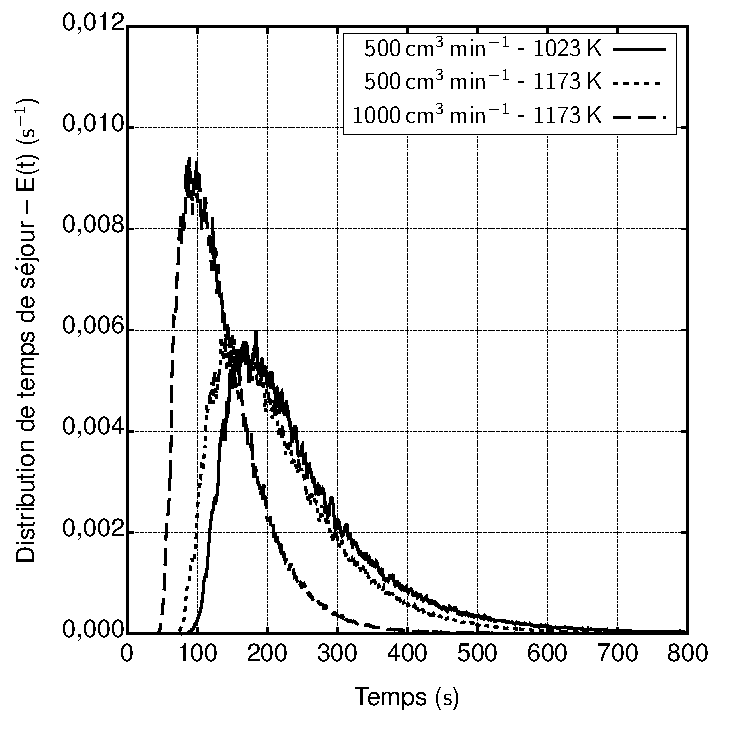
\includegraphics{figures/ch-03-rtd_raw_unloaded}}
  }\hfill
  \subfloat[Réacteur chargé.]{
    \centering\resizebox{0.48\textwidth}{!}{
      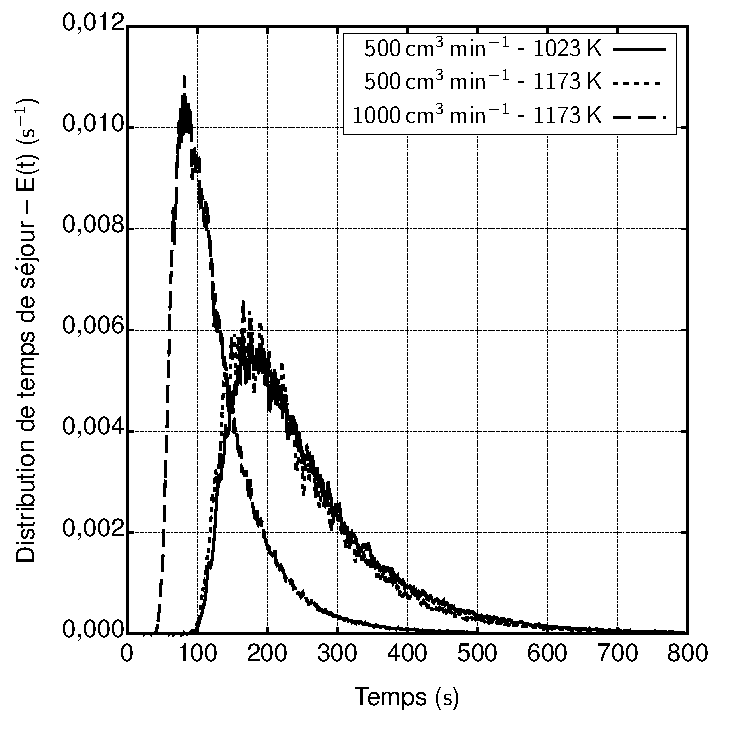
\includegraphics{figures/ch-03-rtd_raw_loaded}}
  }
  
  \caption{\label{fig:residence_time_distribution_raw}Densité de probabilité des distributions du temps de séjour non-normalisées en fonction du temps pour différentes conditions de débit et de température.}
\end{figure}

L'augmentation du débit diminue le temps de séjour moyen $t_{m}$ et réduit aussi la largeur $\sigma$ du pic de la densité de probabilité $E(t_{s})$, ce que l'on vérifie dans le comportement de la grandeur $\sigma$, le moment d'ordre 2 de la distribution, ce qui va à l'encontre des hypothèses définissant des réacteurs du type piston. La Figure~\ref{fig:residence_time_distribution_raw} met en évidence ce comportement du réacteur en fonction des différents débits employés avec et en l'absence d'un échantillon métallique. L'allure de ces courbes se rapproche du comportement d'un réacteur tubulaire laminaire, pour lequel un délai sur l'arrivée des espèces à la sortie produit une montée en intensité assez prononcée \textendash{} composante du comportement de type piston \textendash{} suivie d'une décroissance d'allure exponentielle \textemdash{} composante du comportement de type réacteur agité. À une température donnée, ce comportement est plus évident pour des débits plus élevés \textemdash{} le gaz est contraint de traverser le
réacteur sur une durée plus courte.

Si l'on compare les intégrales normalisées des courbes de la Figure~\ref{fig:residence_time_distribution_raw} tracées en fonction du temps réduit (Figure~\ref{fig:residence_time_distribution_integrated}) avec le comportement théorique (Figure~\ref{fig:types_de_reacteur}), on observe que le réacteur adopte un comportement approximativement du type laminaire. Les conditions expérimentales employées conduisent à des nombres de Reynolds de l'ordre de l'unité à la pression atmosphérique. Les traitements sous vide mènent à des valeurs beaucoup plus faibles et donc l'écoulement doit aussi être laminaire. Le nombre de Knudsen estimé Section~\ref{sec:cinetique} assure un comportement du type visqueux dans les deux limites de pression étudiées. Les courbes intégrées et normalisées (Figure~\ref{fig:residence_time_distribution_integrated})  montrent~\cite{Fogler1999} que dans la plage de débits étudiée, le réacteur conserve le même type de comportement. Le chargement du réacteur à la température de traitement avec des pièces métalliques agit quant à lui dans le sens d'une faible augmentation du temps de séjour  moyen. Lorsque l'effet du chargement avec des échantillons de même taille que ceux qui sont utilisés pour les études métallurgiques ne produit pas de changement important de $t_{m}$, on se contente alors de réaliser les études expérimentales sur la pyrolyse de l'acétylène et de l'ammoniac sans échantillon. Cela permet aussi de séparer les effets de catalyse sur les surfaces métalliques des phénomènes ayant lieu dans le gaz ou sur les parois du réacteur.

\begin{figure}[h]
  \centering
  \subfloat[Réacteur non-chargé.]{
    \centering\resizebox{0.48\textwidth}{!}{
    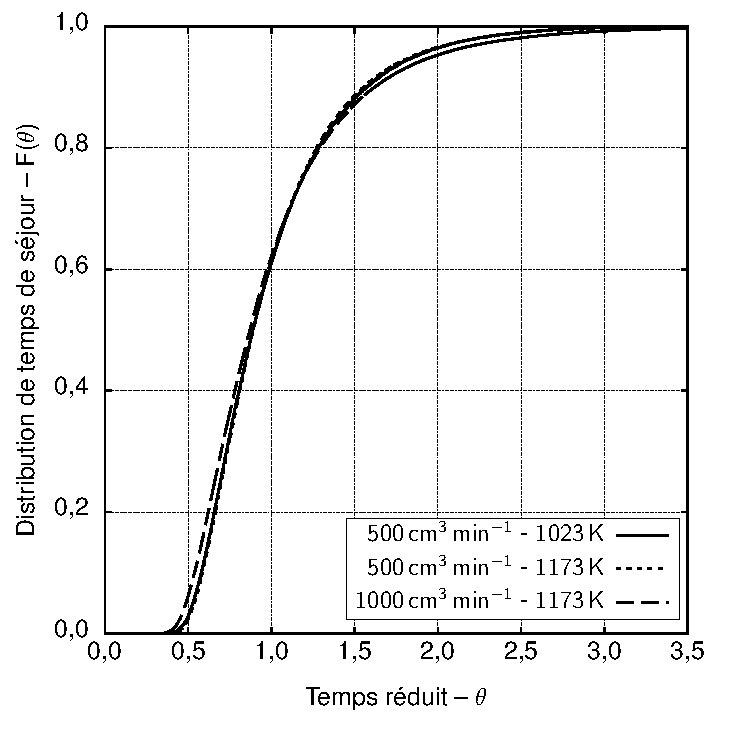
\includegraphics{figures/ch-03-rtd_unloaded}}
  }\hfill
  \subfloat[Réacteur chargé.]{
    \centering\resizebox{0.48\textwidth}{!}{
    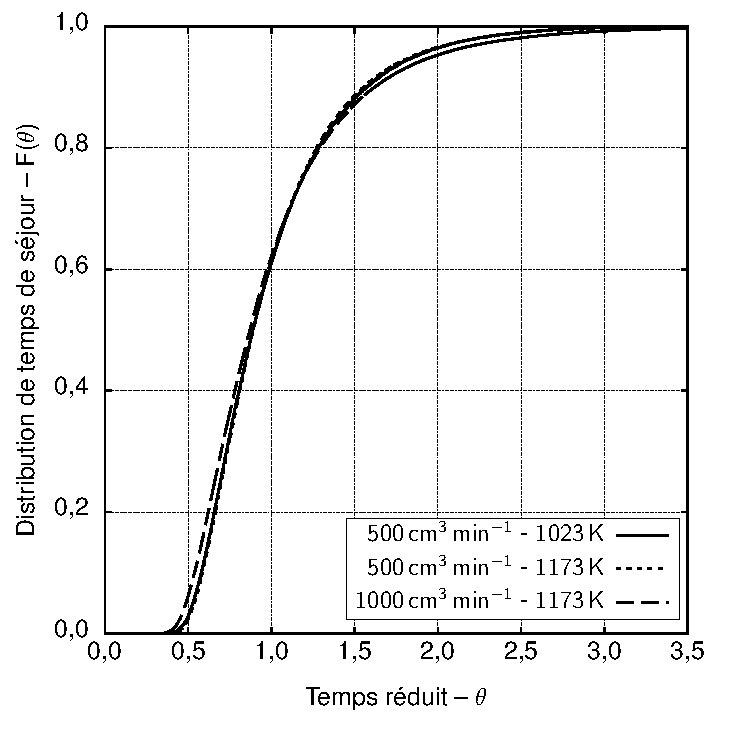
\includegraphics{figures/ch-03-rtd_loaded}}
  }

  \caption{\label{fig:residence_time_distribution_integrated}Distributions du temps de séjour intégrées et normalisées en fonction du temps réduit $\theta$. Les courbes sont identifiées par les conditions de débit et de température.}
\end{figure}

Le comportement de mélange des nouveaux éléments de volume arrivant dans l'enceinte du réacteur peut être caractérisé par les nombres de Bodenstein ou de Peclet axial~\cite{Becker1998177,Fogler1999}.  Les définitions de ces nombres sont présentées Équation~\ref{eq:bodenstein_peclet}, où $D$ désigne le coefficient de diffusion moléculaire, $d$ le diamètre du tube, $L$ sa longueur et $\bar{\nu}$ la vitesse moyenne. Une valeur élevée ($Bo{}\geq{}50$) implique un comportement de ségrégation \textendash{} les nouveaux volumes rentrant dans le réacteur ne sont pas dilués dans le contenu de l'enceinte~\cite{Becker1998177} \textendash{} tandis qu'un réacteur agité possède un nombre de Bodenstein réduit. Ce critère n'est valable que pour des ratios $\nicefrac{L}{d}\geq40$ et son utilisation directe produit une incertitude importante. Dans ce cas, l'ajustement des distributions expérimentales au moyen de l'Équation~\ref{eq:rtd_bodenstein} conduit à des résultats plus fiables~\citep{Becker1998177}.

\begin{equation}
  Pe_{ax}=\frac{192D}{\bar{\nu}d}\quad\quad\quad 
  Bo=Pe_{ax}\frac{L}{d}
  \label{eq:bodenstein_peclet}
\end{equation}

\begin{equation}
  E(\theta)=\frac{1}{2}\sqrt{\frac{Bo}{\pi\theta}}
    \biggr[\exp\biggr(\frac{(1-\theta)^{2}Bo}{4\theta}\biggr)\biggr]^{-1}
  \label{eq:rtd_bodenstein}
\end{equation}

Les valeurs ainsi obtenues pour le nombre de Bodenstein (Tableau~\ref{tab:temps_caracteristics}) montrent que le chargement et/ou l'augmentation du débit conduisent à l'augmentation de l'effet de mélange dans le réacteur. Pour des valeurs de l'ordre de 5, le comportement de mélange ne peut pas être considéré comme étant ségrégé.  Ces estimations ne sont valables que pour le méthane, mais l'ordre de grandeur et le type de comportement restent inchangés pour d'autres espèces, en raison de la proximité des valeurs des coefficients de diffusion des hydrocarbures légers et de celles des dérivés de l'ammoniac dans les gaz utilisés~\footnote{Pour leurs sections de collision, voir \citet{Bird}, par exemple.}.  
Alors que la valeur de $t_{m}$ est associée aux taux d'avancement des réactions globales de décomposition des gaz précurseurs et donc au comportement du réacteur à l'état stationnaire, c'est la valeur de $t_{\infty}$ qu'il convient de considérer pour connaitre le temps nécessaire au renouvellement de l'atmosphère \textemdash{} ici déterminée pour une valeur de $F(t_{\infty})=0,99$. Cette valeur de $t_{\infty}$ représente donc le temps minimal pour démarrer le suivi de la pyrolyse des atmosphères à l'état stationnaire et aussi le temps nécessaire pour atteindre des enrichissements à concentration constante pour les atmosphères à l'équilibre thermodynamique, comme dans le cas de la cémentation à partir de mélanges \ch{CO-H2}.

\subsection{Chromatographie gazeuse à basse pression}
\label{sec:chromatographie_bp}

La mise au point des traitements thermochimiques demande la connaissance préalable de la cinétique de décomposition des précurseurs pour l'enrichissement des matériaux dans la gamme de pressions étudiée. Pour cela, cette étude comprend des mesures par chromatographie gazeuse des produits issus de la décomposition de l'ammoniac et de l'acétylène. Bien que la chromatographie gazeuse à la pression atmosphérique soit une technique bien connue et employée dans la caractérisation des atmosphères gazeuses, son emploi sous pression réduite n'est pas simple. Cette section décrit la méthode employée pour réaliser l'acquistion des chromatogrammes à basse pression ainsi que les limitations qui doivent être prises en compte dans l'analyse des résultats.

L'acquisition des données à basse pression se fait par un équipement Perkins Elmer modèle Clarus 580 équipé d'une colonne pour la séparation primaire des composants qui sont ensuite divisés dans une colonne Molsieve 5A pour la séparation des composants de la bande atmosphérique (\ch{N2}, \ch{O2}, \ch{CH4}, etc.) et dans une colonne Poraplot U pour l'identification des hydrocarbures et de l'ammoniac. La détection de ces produits se fait par un détecteur du type TCD. Bien qu'il s'agisse d'un système conventionnel de chromatographie gazeuse, le prélèvement de l'échantillon pour l'injection dans les colonnes se fait d'une façon particulière. Le système mis en place est connecté à une des sorties du réacteur employé dans l'étude, laquelle est soumise à un pompage intermittent vers le système de prélèvement à basse pression. L'appareil est composé d'une série de vannes qui permettent le remplissage d'un ballon en élastomère par les produits prélevés à la sortie du réacteur, ballon qui fait office d'enceinte tampon. Après le remplissage du ballon, les gaz ainsi prélevés sont comprimés à la pression atmosphérique puis injectés dans la boucle de prélèvement de l'équipement de chromatographie. La Figure~\ref{fig:systeme_bp} présente un schéma du système de prélèvement, où \og{}$B$\fg{} désigne le ballon d'échantillonnage et \og{}$P$\fg{} la pompe à vide. La séquence d'opérations automatisée du système est fournie Annexe~\ref{an:caracterisation_atmospheres}. %et certains détails complémentaires.

\begin{figure}[h]
  \centering\resizebox{0.6\textwidth}{!}{
    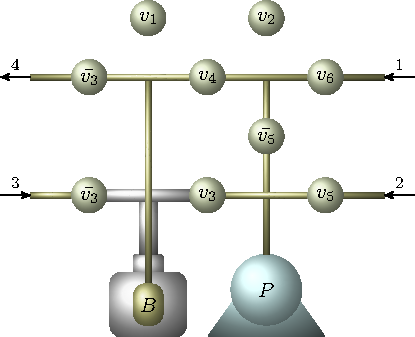
\includegraphics{figures/ch-03-schema_gcbp}}
  
  \caption{\label{fig:systeme_bp}Système de prélèvement à basse pression. Les flèches désignent: 1 -- le prélèvement du réacteur, 2 -- la sortie du système de chromatographie, 3 -- l'entrée d'air pour comprimer l'échantillon et 4 -- l'injection du système de chromatographie.}
\end{figure}

Ce système permet une acquisition reproductible des chromatogrammes au--delà de \SI{30}{\milli\bar} avec l'accumulateur \og{}$B$\fg{} utilisé. Pour travailler à plus faible pression, un accumulateur de volume supérieur est requis. Bien que l'acquisition soit reproductible, elle reste faiblement dépendante de la pression totale du système, impliquant le besoin d'un étalonnage pour chaque pression utilisée dans l'étude. Au moment du détournement du gaz vers l'accumulateur, le réacteur est soumis à des variations momentanées de pression qui sont contrôlées manuellement pendant l'acquisition de l'échantillon. Ces oscillations conduisent à des erreurs relatives de mesure qui peuvent atteindre 10\% entre \SIrange{30}{100}{\milli\bar}. %De plus, étant donné que de faibles admissions des gaz de l'atmosphère dans le réacteur au cours de cette étape, l'étalonnage est limité en précision et dépendant des ce fuites qui sont dépendant naturellement de la pression d'opération.

\section{Cémentation à partir des mélanges \ch{CO-H2}}
\label{sec:classical_carburizing}

Afin d'assurer une saturation de la surface en carbone pour les traitements de cémentation à partir des mélanges gazeux, une étude thermodynamique de l'équilibre gaz--solide a été menée pour chaque alliage. Cela a été fait de manière à employer une méthode basée sur la mesure de la température du point de rosée $T_{r}$ des effluents du réacteur. Le calcul de $T_{r}$ a été réalisé en considérant l'atmosphère de cémentation (Tableau~\ref{tab:treatment_atmospheres}). Les paramètres de \citet{Gunnarson1967} des alliages étudiés sont calculés, conduisant à $Q=1,1$ pour l'alliage 16NiCrMo13 et $Q=0,9$ pour la nuance 23MnCrMo5. Il existe une plus forte affinité avec le carbone pour l'alliage 23MnCrMo5 \textendash{} visible sur la Figure~\ref{fig:dew_point} en fixant une valeur de $T_{r}$: la fraction massique en carbone en équilibre entre le matériau et l'atmosphère est plus élevée pour cette nuance que pour l'alliage 16NiCrMo13. La Figure~\ref{fig:dew_point} compare également les résultats du calcul de $T_{r}$ selon la méthode classique présentée Section~\ref{sec:controle_cementation} à ceux des simulations effectuées avec Thermo-Calc~\cite{Andersson2002,Borgenstam2000} \textendash{} les températures $T_{r}$ à la saturation en carbone dans les alliages diffèrent de moins de \SI{1}{\kelvin} et l'écart entre les méthodes ne dépasse pas \SI{3}{\kelvin} en dessous de cette limite. La divergence des courbes que l'on observe au--delà de la limite de saturation des alliages s'explique par le fait que l'Équation~\ref{eq:ellis_carbone} ne considère pas de transitions de phase. Il est important que la température de point de rosée pendant les traitements ne soit pas inférieure à celle conduisant à la saturation, ce qui peut entrainer une précipitation importante de cémentite. L'Annexe~\ref{an:dew-point} présente les détails de ces simulations.

\begin{table}[h]
  \caption{\label{tab:treatment_atmospheres}Atmosphères pour les étapes de cémentation et de nitruration des traitements réalisés à la pression atmosphérique.}
  
  \centering{}\footnotesize{}%
  \resizebox{\textwidth}{!}{
    \begin{tabular}{\$c^c^c^c^c^c^c}
      \cmidrule[2pt]{1-3}  \cmidrule[2pt]{5-7}  
      \multicolumn{3}{c}{\bfseries Cémentation} 
      & & 
      \multicolumn{3}{c}{\bfseries Nitruration}
      \tabularnewline
      \cmidrule[2pt]{1-3}  \cmidrule[2pt]{5-7}  
      {0,20 \ch{CO}} & {0,40 \ch{H2}} & {0,40 \ch{N2}} 
      & & 
      {0,04 \ch{NH3}} & {0,72 \ch{H2}} & {0,24 \ch{N2}}
      \tabularnewline[6pt]
      %
      {\SI{100}{\sccm}} & {\SI{200}{\sccm}} & {\SI{200}{\sccm}} 
      & & 
      {\SI{15}{\sccm}} & {\SI{300}{\sccm}} & {\SI{100}{\sccm}}
      \tabularnewline
      \cmidrule{1-3}  \cmidrule{5-7} 
    \end{tabular}
  }
\end{table}

\begin{figure}[!ht]
  \centering
  \subfloat[Alliage 16NiCrMo13.]{
    \centering\resizebox{0.48\textwidth}{!}{
    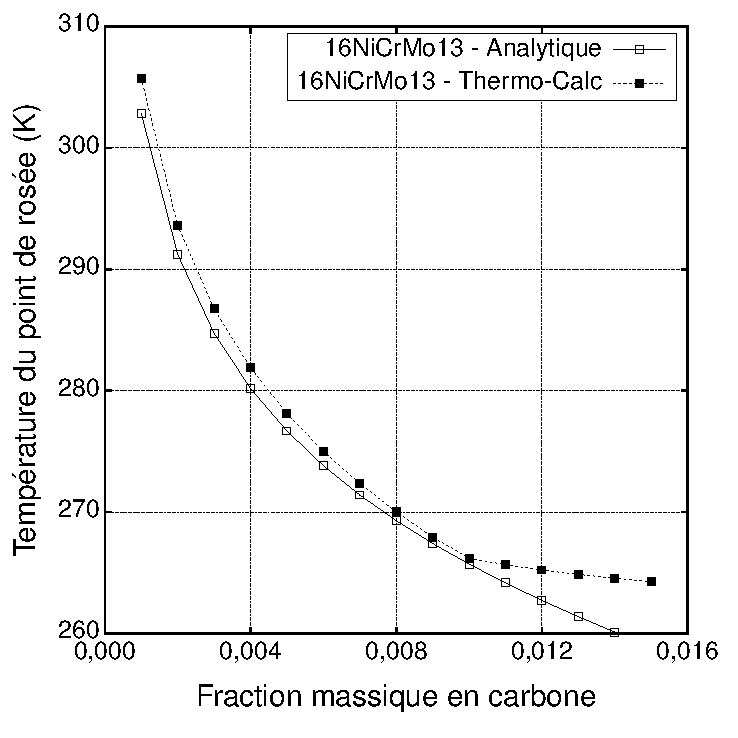
\includegraphics{figures/ch-03-dew_point_aero}}
  }\hfill
  \subfloat[Alliage 23MnCrMo5.]{
    \centering\resizebox{0.48\textwidth}{!}{
    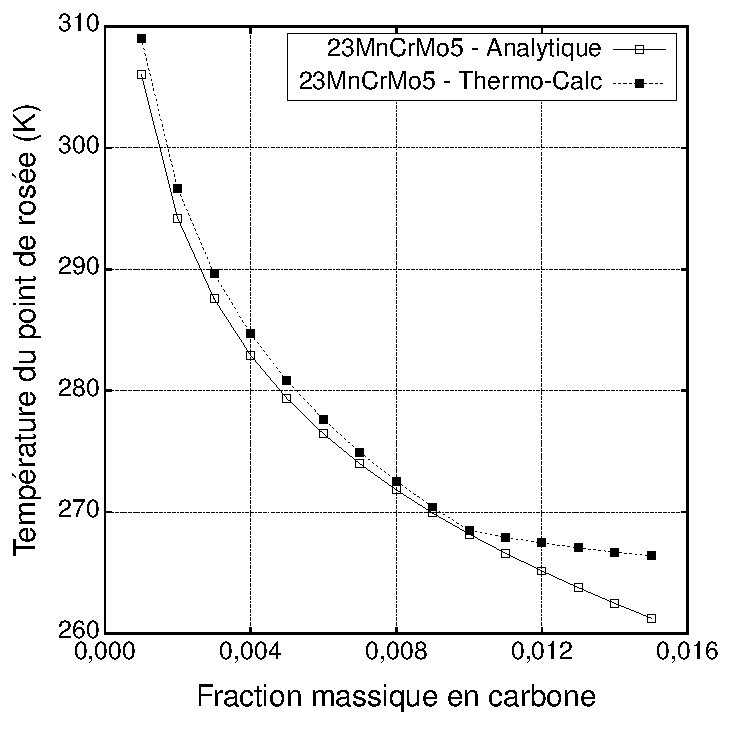
\includegraphics{figures/ch-03-dew_point_auto}}
  }

  \caption{\label{fig:dew_point}Température du point de rosée en fonction de la fraction massique en carbone à l'équilibre avec l'atmosphère de traitement.}
\end{figure}

\section{Procédés à partir des hydrocarbures}
\label{sec:pyrolyse_acetylene}

L'étude de la pyrolyse de l'acétylène, précurseur du carbone pour l'étape de cémentation, s'est faite par chromatographie en phase gazeuse. Les mesures effectuées visent à fournir des indications sur les espèces présentes dans le réacteur pour le transfert de matière vers le solide, sur les mécanismes de surface régissant les traitements évalués et sur la validité des mécanismes développés. L'étude des réactions de surface s'opère généralement par une analyse différentielle des produits obtenus en l'absence et en présence d'un échantillon. Pour cela, on suppose que la réactivité des parois en alumine du réacteur est négligeable par rapport aux effets induits par les surfaces des éprouvettes métalliques.  On commence donc par étudier le réacteur non-chargé. Les paramètres de contrôle pris en compte pour l'étude sont le débit total, le débit du précurseur étudié et la température. % dans la zone de contrôle du réacteur.

\subsection{Pyrolyse à la pression atmosphérique}

Les expériences à la pression atmosphérique ont été réalisées en employant \ch{N2} comme gaz porteur et ont permis le suivi de la pyrolyse de l'acétylène dans la plage de température allant de \SIrange{873}{1223}{\kelvin}. Afin d'établir une pression partielle de \ch{C2H2} de l'ordre de \SI{20}{\hecto\pascal}, pression de référence dans cette étude pour les traitements à basse pression, un mélange contenant \ch{N2 - 0,02 C2H2} en fraction volumique a été employé, et ce pour des débits de \SIlist{500;1000}{\cubic\centi\metre\per\minute}. Ces conditions sont résumées Tableau~\ref{tab:pyrolysis-conditions-pa}. La caractérisation de cette atmosphère en sortie du réacteur a permis la quantification des hydrocarbures légers \ch{CH4}, \ch{C2H2} et \ch{C2H4} et \ch{H2} à l'aide du détecteur FID du chromatographe. L'acquisition des données s'est faite toutes les \SI{20}{\minute} pour les hydrocarbures et toutes les \SI{4}{\minute} pour \ch{H2}, qui est mesuré par le détecteur TCD. 

\begin{table}[h]
  \caption{\label{tab:pyrolysis-conditions-pa}Conditions expérimentales pour l'étude de la pyrolyse du \ch{C2H2} à pression atmosphérique dans le réacteur présenté Figure~\ref{fig:reacteur_pa}.}
  
  \resizebox{\textwidth}{!}{
  \footnotesize{}\centering{}
  \begin{tabular}{\$c^c^c^c^c}
    \toprule[2pt]
    \rowstyle{\bfseries}
    Température 
    & Débit 
    & Mélange 
    & Pression totale 
    & Pression \ch{C2H2}
    \tabularnewline
    \midrule[2pt]
    \SIrange{873}{1223}{\kelvin} 
    & \SIlist{500;1000}{\sccm}
    & \ch{N2 - 0,02 C2H2}
    & \SI{1000}{\hecto\pascal}
    & \SI{20}{\hecto\pascal}
    \tabularnewline
    \bottomrule
  \end{tabular}
  }
\end{table}

Les fractions molaires des espèces identifiées à l'état stationnaire sont présentées Figure~\ref{fig:acetylene_pyrolysis} en fonction de la température de la zone chaude du réacteur. On vérifie que même pour des temps de séjour supérieurs à \SI{100}{\second}, l'acétylène est l'hydrocarbure léger majoritaire. En dessous de \SI{900}{\kelvin} le craquage de \ch{C2H2} est négligeable par rapport à la concentration injectée dans le réacteur et l'étude se limite à des mesures au--dessus de \SI{873}{\kelvin}. On observe aussi le rôle du temps de séjour : à une température donnée, une augmentation du débit produit une plus faible conversion du gaz source en sous-produits, tel qu'on peut le mettre en évidence pour les températures de \SIrange{1023}{1223}{\kelvin} en comparant les fractions de \ch{C2H2} et \ch{H2}, et est équivalente à un décalage de \SI{50}{\kelvin} dans\textsl{} la zone chaude du réacteur. %Pour les distributions de temps de séjour de la Figure~\ref{fig:residence_time_distribution_raw}, cette augmentation de débit est équivalente à une décalage de \SI{50}{\kelvin} dans la température de la zone chaude du réacteur.

\begin{figure}[!ht]
  \centering
  \subfloat[Toutes les espèces.]{
    \centering\resizebox{0.98\textwidth}{!}{
      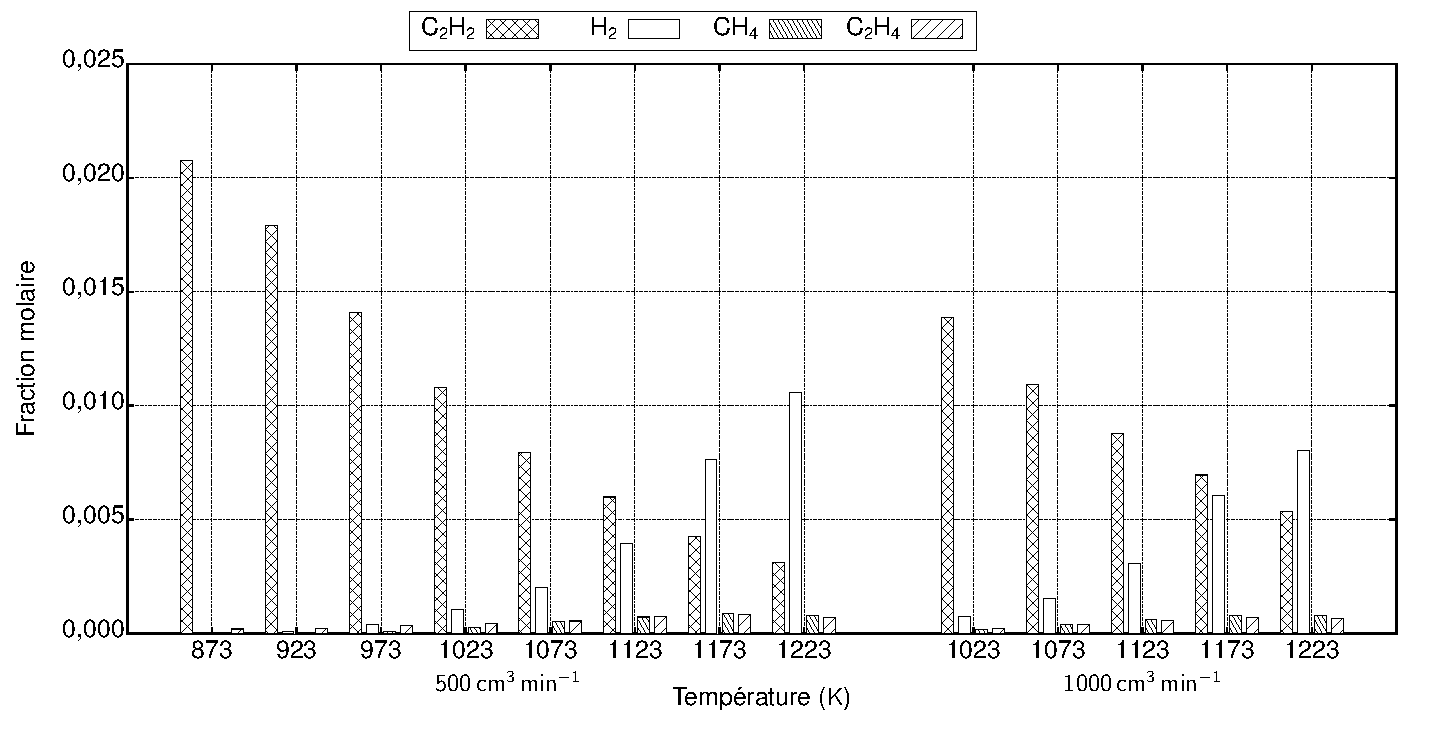
\includegraphics{figures/ch-03-decomposition_c2h2_all_pa}}
  }\\
  \subfloat[Espèces minoritaires.]{
    \centering\resizebox{0.98\textwidth}{!}{
      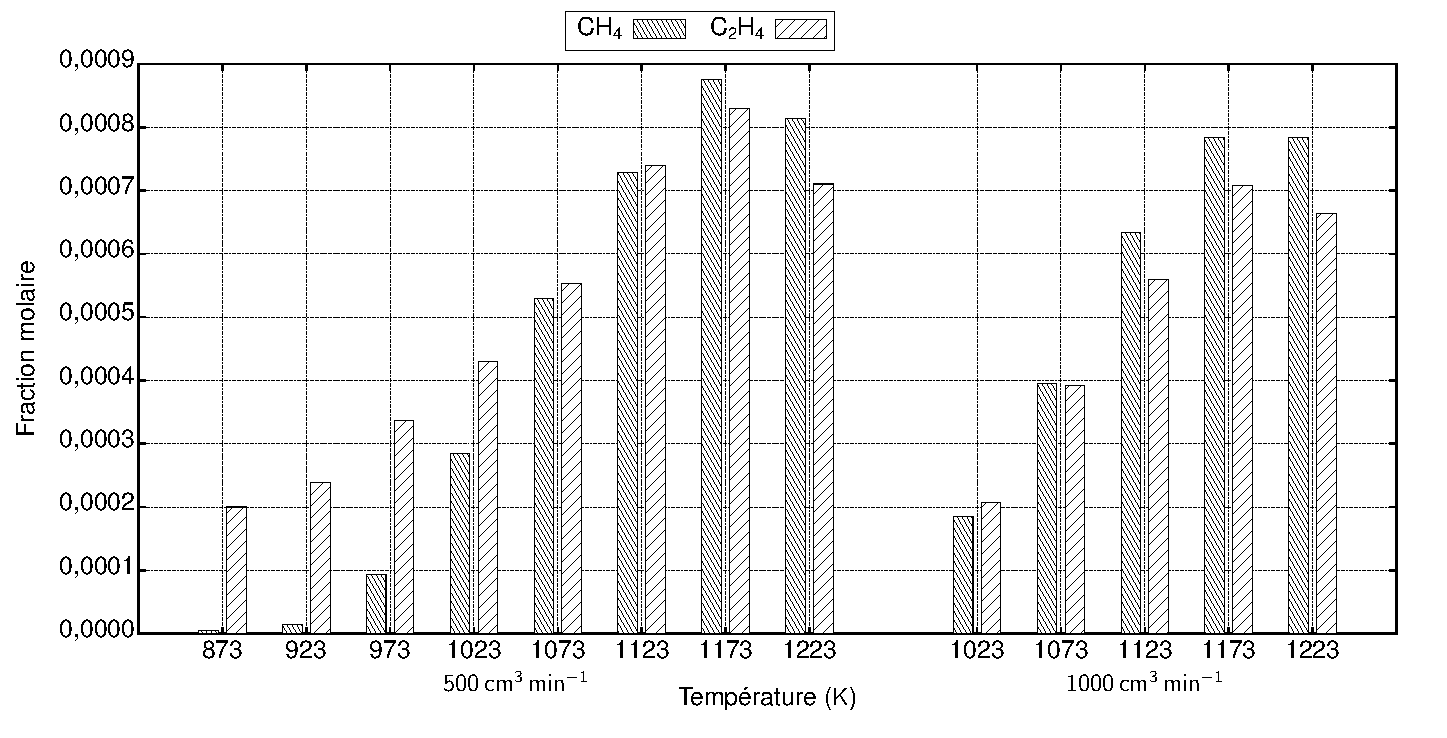
\includegraphics{figures/ch-03-reaction_byproducts_pa}}
  }
  
  \caption{\label{fig:acetylene_pyrolysis}Suivi des produits de pyrolyse de l'acétylène à la pression atmosphérique en fonction de la température de la zone chaude du réacteur. Les produits mesurés sont fonctions des interactions entre le gradient de température et la distribution $E(t_{s})$ pour les débits de \SIlist{500;1000}{\sccm}.}
\end{figure}

Selon les données du Tableau~\ref{tab:temps_caracteristics}, l'augmentation du débit de \SIrange{500}{1000}{\sccm} n'a pas seulement réduit le temps de séjour moyen à l'intérieur du four, mais a aussi diminué la largeur du pic de densité de probabilité, les deux effets combinés conduisant aux réponses mesurées. %Une autre manière de décrire ce comportement, consiste à dire que l'augmentation du débit diminue la valeur de $Bo$, ce qui favorise le comportement de mélange dans le réacteur et permet donc que le précurseur sorte plus tôt du réacteur. 
Il faut aussi tenir compte du fait que la pyrolyse se passe dans une zone comportant un gradient de température si bien que les produits analysés proviennent de différentes zones du réacteur. La réduction de la température de la zone chaude implique aussi l'augmentation du temps de séjour avec un élargissement du pic de la $E(t_{s})$.  Étant donné que les temps de séjour sont beaucoup plus longs que ceux employés par~\citet{Norinaga2005,Norinaga2007}, il en résulte que la décomposition de l'acétylène et la formation de \ch{CH4} et \ch{C2H4} sont beaucoup plus avancées. Ces résultats se rapprochent des observations faites par \citet{Graf2007} et \citet{Khan2008}.

Le bilan matière des espèces rapportées sur la Figure~\ref{fig:acetylene_pyrolysis} n'atteint pas l'unité: il est donc possible d'estimer la composition des espèces inconnues dans le système et la fraction qu'elles représentent. Tout d'abord, on calcule l'apport de chaque espèce mesurée $\phi$ à la fraction des atomes $i$ composant le système \textendash{} le carbone et l'hydrogène \textendash{} récupérés à la sortie. Cette contribution $\psi_{i,\phi}$ s'exprime selon $\psi_{i,\phi}=n_{i,\phi}\times x_{\phi}$, où $n_{i,\phi}$ désigne le nombre d'atomes de $i$ dans $\phi$ et $x_{\phi}$ la fraction molaire mesurée de cette espèce. La fraction d'atomes $i$ récupérée à la sortie par rapport à celle à l'entrée, que l'on notera $\Psi_{i}$, est définie par le rapport entre les sommes des $\psi_{i,\phi}$ à la sortie et à l'entrée du réacteur.  Pour le carbone et l'hydrogène, grâce aux données acquises, on peut écrire les Équations~\ref{eq:psi_c}~et~\ref{eq:psi_h}, respectivement, où les numérateurs sont des sommes pondérées des fractions molaires des produits à la sortie et les dénominateurs la fraction molaire du précurseur à l'entrée. L'hypothèse de débit volumique constant est raisonnable compte tenu de la dilution du mélange à l'entrée et du comportement de pyrolyse de l'acétylène~\cite{Norinaga2005}.

\begin{equation}
  \Psi_{\ch{C}}=\dfrac{1\times x_{\ch{CH4},s}+2\times x_{\ch{C2H2},s}+2\times x_{\ch{C2H4},s}+0\times x_{\ch{H2},s}}{2\times x_{\ch{C2H2},e}}
  \label{eq:psi_c}
\end{equation}

\begin{equation}
  \Psi_{\ch{H}}=\dfrac{4\times x_{\ch{CH4},s}+2\times x_{\ch{C2H2},s}+4\times x_{\ch{C2H4},s}+2\times x_{\ch{H2},s}}{2\times x_{\ch{C2H2},e}}
  \label{eq:psi_h}
\end{equation}

Indépendamment de cette approche, on vérifie Figure~\ref{fig:balance_molaire} que dans la plage de température typique de la cémentation/carbonitruration \textendash{} \SIrange{1173}{1223}{\kelvin} \textendash{} il reste moins de 30\% de carbone sous forme d'hydrocarbures légers pour tous les débits considérés.  Environ 70-80\% du carbone se trouve sous forme d'hydrocarbures plus lourds ou de suies non mesurées. Ces courbes permettent aussi d'identifier la fraction des atomes d'hydrogène présents dans des hydrocarbures non-mesurés. Contrairement au carbone, à haute température, la localisation de l'hydrogène dans des molécules est connue à environ 80\%. Dans tout le domaine de température balayé, la fraction d'hydrogène présente dans les hydrocarbures est inférieure à celle sous forme de \ch{H2}.

\begin{figure}[!ht]
  \centering
  \subfloat[\label{fig:bilan-atomique-pa}Bilan atomique.]{
    \centering\resizebox{0.98\textwidth}{!}{
      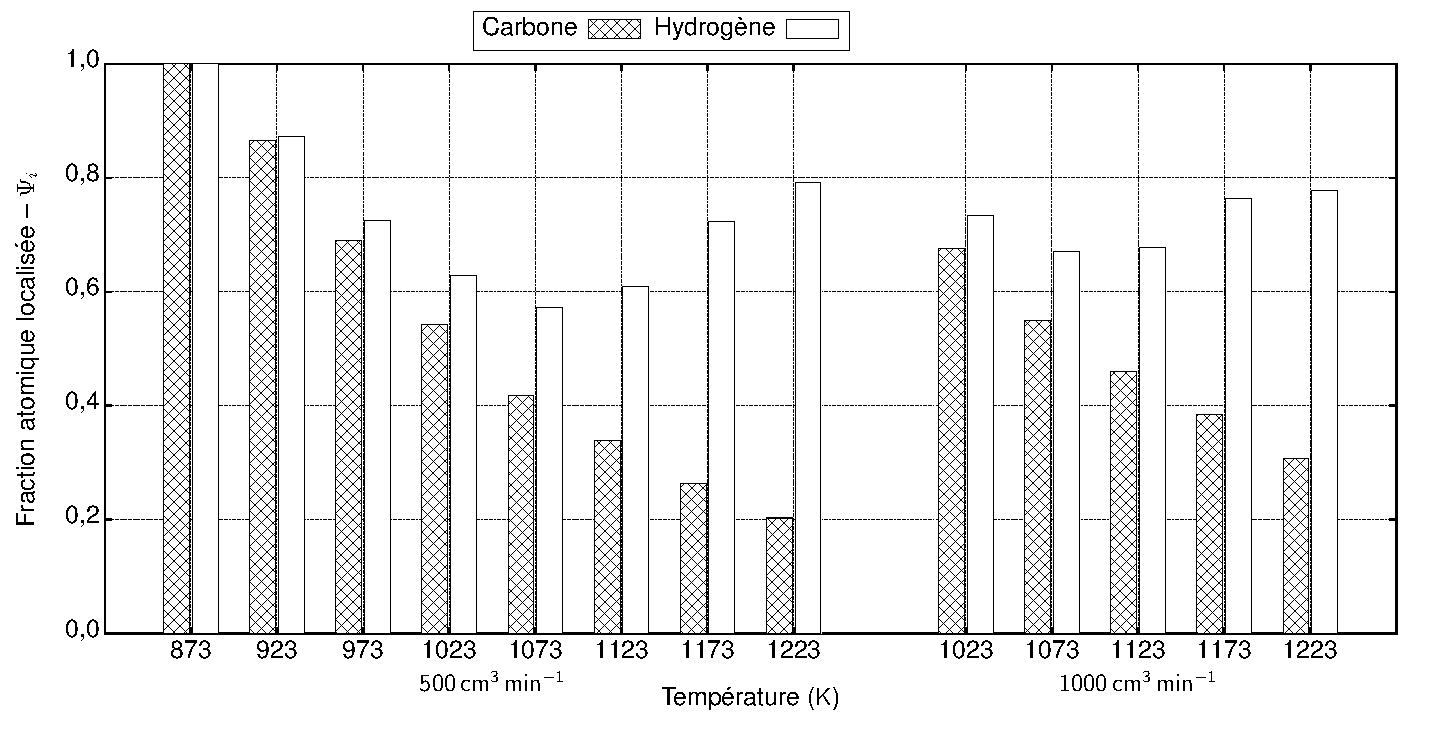
\includegraphics{figures/ch-03-balance_molaire}}
  }\\
  \subfloat[\label{fig:ration_ch}Rapport $\nicefrac{\ch{C}}{\ch{H}}$.]{
    \centering\resizebox{0.98\textwidth}{!}{
      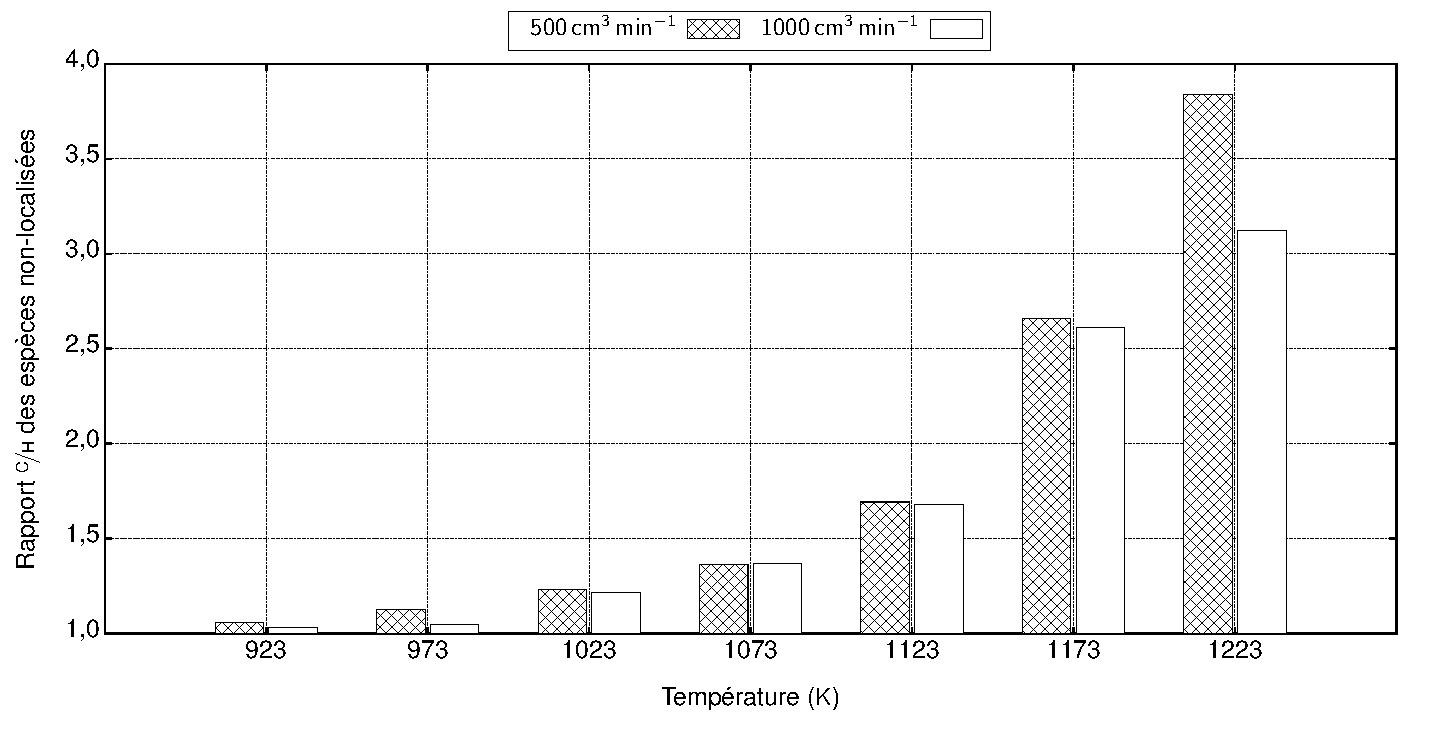
\includegraphics{figures/ch-03-ratio_carbon_hydrogen}}
  }

  \caption{\label{fig:balance_molaire}Bilan matière de la pyrolyse de l'acétylène à la pression atmosphérique réalisé à partir des données de la Figure~\ref{fig:acetylene_pyrolysis} et rapport  calculé entre le nombre d'atomes de carbone et d'hydrogène dans les espèces non-détectées.}
\end{figure}

On observe (Figure~\ref{fig:ration_ch}) que le rapport $\nicefrac{\ch{C}}{\ch{H}}$ des espèces inconnues augmente dans la plage de température étudiée, ce qui implique une réduction des saturations dans les hydrocarbures.  Par exemple, sur plus de 200 espèces présentes dans le mécanisme cinétique compilé par \citet{Norinaga2007}, à peine une dizaine d'entre elles possèdent un ratio $\nicefrac{\ch{C}}{\ch{H}}\geq2,0$, à savoir celles de la famille du coronène. La majorité des composants aromatiques légers se situe entre 1,0 et 2,0. Le benzo(a)pyrène, composant indésirable pour des raisons de santé, présente un rapport $\nicefrac{\ch{C}}{\ch{H}}=1,67$. Les ratios au-delà de 3,0 représentent des radicaux riches en carbone (\ch{C3H}, \ch{C6H}, etc.) ou des dépôts de suie issus de la pyrolyse.  Au--dessus de \SI{1123}{\kelvin} ce ratio croît rapidement, condition pour laquelle la pollution du four et la formation de dépôts est favorisée.

\subsection{Pyrolyse sous pression réduite}
\label{sec:pyrolyse_acetylene_bp}

La cinétique de pyrolyse de l'acétylène a été étudiée à basse pression en utilisant le réacteur décrit Section \ref{sec:reacteur_bp}. Ces expériences ont été réalisées dans la plage de pressions entre \SIrange{30}{100}{\hecto\pascal} en utilisant un mélange \ch{N2 - 0,36 C2H2} sous un débit de \SI{222}{\sccm} \textemdash{} Tableau~\ref{tab:pyrolysis-conditions-bp}. Les résultats de ces mesures se trouvent Figure~\ref{fig:pyrolyse_acetylene_bp}. L'étalonnage du système a été réalisé à la pression de \SI{50}{\milli\bar} et complété par des vérifications aux pressions limites utilisées dans l'expérience. Le système de compression permet un remplissage complet de la boucle de prélèvement du chromatographe à partir de \SI{30}{\milli\bar} et la calibration est indépendante de la pression. Cela n'empêche pas l'utilisation de ce système en dessous de \SI{30}{\milli\bar}, mais dans ce cas un étalonnage doit être réalisé pour chaque pression utilisée et les résultats sont beaucoup moins reproductibles en dessous de ce seuil d'opération. %~\footnote{En outre, du fait de la perturbation causée par le système de pompage pendant le prélèvement de l'échantillon, les résultats sont beaucoup moins reproductibles en dessous de ce seuil d'opération.}. %L'oxygène résiduel a été inclus dans le bilan matière en utilisant une correction de la courbe d'étalonnage du di-azote ce qui est possible en raison de leurs diffusivités thermiques assez proches~\footnote{Conductivité égale à \SI{38,8}{\milli\watt\per\metre\per\kelvin} pour \ch{N2} contre \SI{40,1}{\milli\watt\per\metre\per\kelvin} pour \ch{O2} à une température de \SI{500}{\kelvin}~\cite{Lienhard2008}, i.e. de l'ordre de celle du détecteur TCD.  Ces espèces présentent des capacités calorifiques de \SI{1055}{\joule\per\kilo\gram\per\kelvin} et \SI{972}{\joule\per\kilo\gram\per\kelvin}, ce qui conduit au rapport entre les diffusivités thermiques $\nicefrac{\alpha_{\ch{O2}}}{\alpha_{\ch{N2}}}=1,12$.}. Cela confirme la présence des traces de \ch{O2}, de l'ordre de \SI{1000}{ppm} dans la bouteille de \ch{N2} et permet l'identification jusqu'à 2\% du flux d'espèces provenant de l'atmosphère extérieure donnée des fuites de l'installation.

\begin{table}[h]
  \caption{\label{tab:pyrolysis-conditions-bp}Conditions expérimentales pour l'étude de la pyrolyse du \ch{C2H2} à basse pression dans le réacteur présenté Figure~\ref{fig:reacteur_bp}.}
  
  \footnotesize{}\centering{}
  \begin{tabular}{\$c^c^c^c^c}
    \toprule[2pt]
    \rowstyle{\bfseries}
    Température 
    & Débit 
    & Mélange 
    & Pression totale 
    & Pression \ch{C2H2}
    \tabularnewline
    \midrule[2pt]
    \SIrange{773}{1273}{\kelvin}
    & \SI{222}{\sccm}
    & \ch{N2 - 0,36 C2H2}
    & \SIrange{30}{100}{\hecto\pascal}
    & \SIrange{10,8}{36,0}{\hecto\pascal}
    \tabularnewline
    \bottomrule
  \end{tabular}
\end{table}

\begin{figure}[!ht]
  \centering
  \subfloat[\label{fig:acetylene_bp}Acétylène.]{
    \centering\resizebox{0.98\textwidth}{!}{
      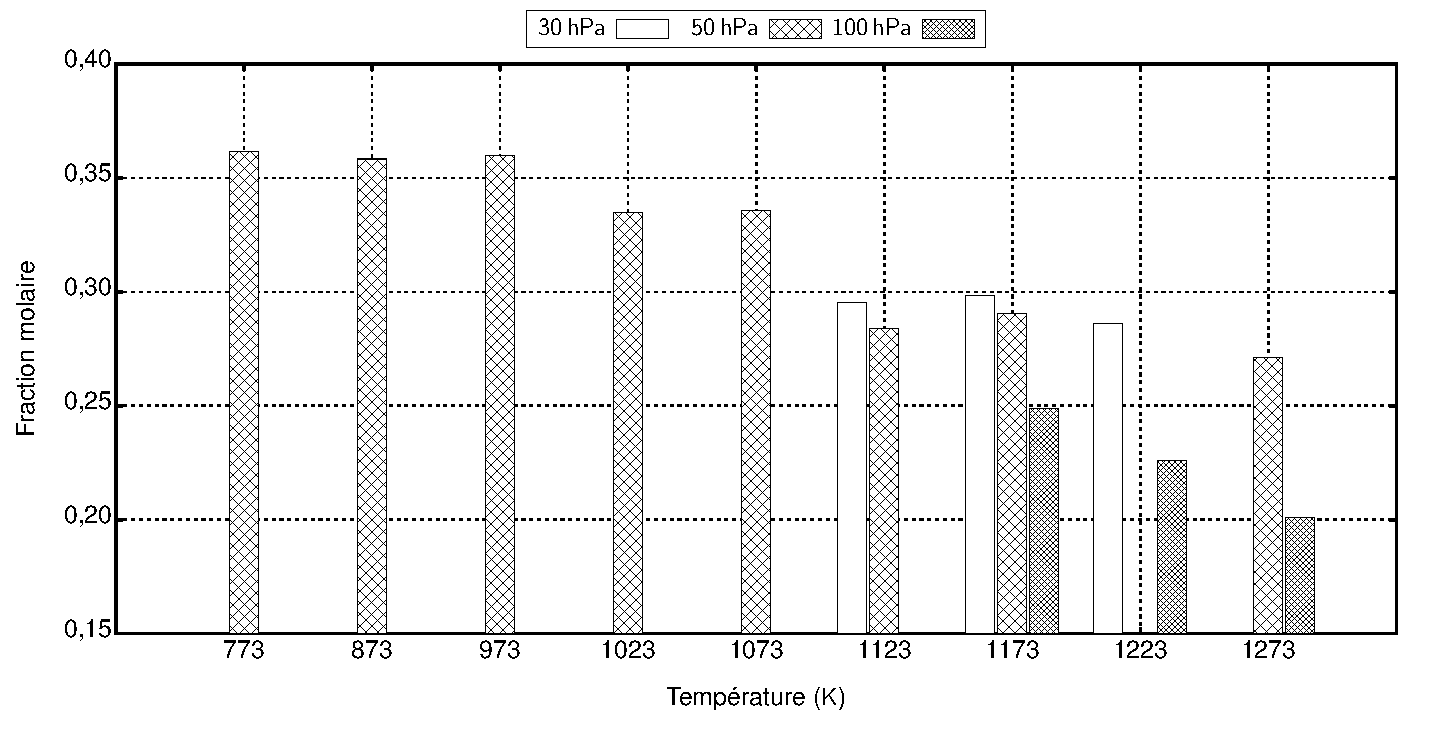
\includegraphics{figures/ch-03-decomposition_c2h2_bp}}
  }\\
  \subfloat[\label{fig:minoritaires_bp}Espèces minoritaires (qualitatif).]{
    \centering\resizebox{0.98\textwidth}{!}{
      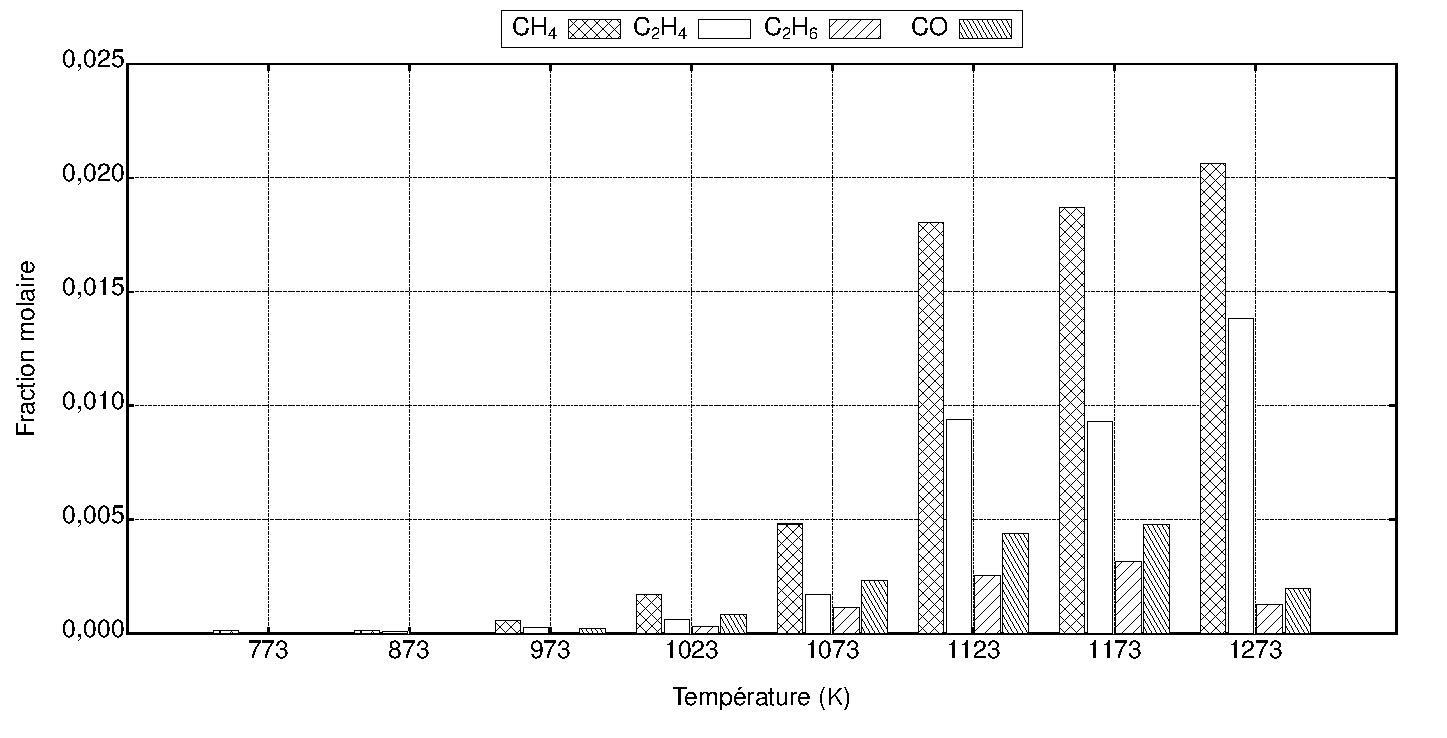
\includegraphics{figures/ch-03-reaction_byproducts_bp}}
  }

  \caption{\label{fig:pyrolyse_acetylene_bp}Pyrolyse du \ch{C2H2} à basse pression dans réacteur horizontal en quartz sous un débit total de \SI{222}{\sccm}: suivi \protect\subref{fig:acetylene_bp} de l'acétylène à la sortie en fonction de la température de contrôle et de la pression d'opération et \protect\subref{fig:minoritaires_bp} des espèces minoritaires à \SI{50}{\hecto\pascal}.}
\end{figure}

On observe Figure~\ref{fig:pyrolyse_acetylene_bp} qu'aucune décomposition du \ch{C2H2} n'a lieu jusqu'à une température de \SI{973}{\kelvin} pour les temps de séjour imposés par le débit total employé. La décomposition commence à devenir importante à partir de \SI{1123}{\kelvin}, température pour laquelle la fraction en acétylène à la sortie correspond à 86\% de celle injectée en entrée. On remarquera que cette valeur ne correspond pas exactement à une conversion de 14\% si l'on prend en compte le changement de volume molaire du gaz. Comme la décomposition ne peut pas être représentée par une réaction globale simple, comme cela est possible pour l'ammoniac, et que par ailleurs l'installation expérimentale utilisée ne comporte pas de système de mesure de débit en sortie, seule une estimation numérique, basée sur nos modèles, du taux de dissociation sera proposée. Les teneurs en \ch{CO} observées sont cohérentes avec la composition nominale de la bouteille \textendash{} le \ch{CO} est issu de l'acétone qui sert à stabiliser l'acétylène \textendash{} comme cela avait déjà été rapporté par \citet{Norinaga2005}. L'influence de la pression présentée Figure~\ref{fig:pyrolyse_acetylene_bp} s'avère être en accord avec la loi d'action de masse. Il faut préciser que la technique de prélèvement induit des difficultés posées par les variations \textendash{} augmentation \textendash{} de pression que l'on observe à \SI{30}{\hecto\pascal}, ce qui peut expliquer la proximité entre les résultats à \SIlist{30;50}{\hecto\pascal} Figure~\ref{fig:acetylene_bp}. Les fractions molaires en hydrocarbures fournies Figure~\ref{fig:minoritaires_bp} sont calculées à partir des intensités relatives des pics mesurés, aucun étalonnage n'étant réalisé~\footnote{Les intensités sont affectées à partir des diffusivités thermiques calculées~\cite{Lienhard2008}: l'estimation est faite en multipliant le facteur d'étalonnage de \ch{C2H2} par le rapport entre la diffusivité de l'espèce considérée et celle de l'acétylène. Le \ch{CO} a été étalonné normalement.}. Ces résultats seront comparés aux prédictions du modèle numérique présenté Chapitre~\ref{ch:modelisation_cinetique}.

\subsection{Cémentation à partir des hydrocarbures}
\label{sec:cementation-hydrocarbure}

La cémentation à partir des hydrocarbures présente quelques particularités par rapport à celle réalisée avec des mélanges \ch{CO-H2}. Les procédés qui utilisent \ch{C2H2} ou \ch{C2H4} comme source de carbone sont régis par la cinétique de catalyse de ces précurseurs et ses produits de décomposition homogène sur les surfaces traitées. La capacité de ces atmosphères de libérer des atomes de carbone est élevée, ce qui implique des potentiels carbone importants. En raison de la cinétique rapide des processus chimiques en phase gazeuse et hétérogènes, la mise au point de la cémentation à partir des hydrocarbures ne peut pas être traitée de la même façon que les procédés proches de l'équilibre, comme les atmosphères \ch{CO-H2}. \citet{Kula2005} ont montré l'importance relative des espèces constituant la couche d'espèces adsorbées formée en utilisant une atmosphère \ch{C2H2}/\ch{C2H4} dilué dans \ch{H2} sans qu'un dépôt carboné soit formé. Les auteurs~\cite{Kula2005} ont observé une faible concentration de radicaux \ch{C1}~\footnote{On notera \ch{C_{$n$}} l'ensemble de composés contenant $n$ atomes de carbone.} avec un maximum de concentration associé aux radicaux de la famille \ch{C2} suivi par une décroissance presque linéaire de l'importance des complexes adsorbés jusqu'à \ch{C7}, lesquels présentent une intensité très réduite. Ces résultats suggèrent l'importance des hydrocarbures légers dans la cémentation réalisée en pulses et donc l'intérêt d'éviter leur consommation dans l'atmosphère. Si l'enrichissement est réalisé avec un flux continu d'hydrocarbures, un dépôt carboné est normalement formé en surface. 
Bien que dans la pratique industrielle de la cémentation consiste en un enrichissement réalisé par pulses d'hydrocarbures pendant une durée de \SIrange{1}{5}{\minute}, en raison de notre installation expérimentale, nous avons tout de même choisi de réaliser des enrichissements en un flux continu. Cette pratique a un effet négligeable sur l'enrichissement de l'alliage en raison du dépôt carboné qui agit à haute température comme une source du carbone: des résultats similaires sont obtenus soit en imposant une condition contrôlée par la cinétique de surface soit en travaillant à concentration constante (dépôt carboné), ce qui permet de contrôler dans chaque cas l'enrichissement par le solide~\cite{Kula2005}. Une étude similaire réalisée par \citet{Gorockiewicz2010429} suggère que le dépôt carboné en surface est composé de graphite.

\subsubsection{Traitements à pression atmosphérique}

La dynamique d'enrichissement en carbone à partir des hydrocarbures à pression atmosphérique a été étudiée uniquement pour l'alliage 23MnCrMo5 à partir du suivi de prise de masse tout au long des traitements de cémentation. Ces traitements ont été réalisés à une température fixe de \SI{1173}{\kelvin} à la pression atmosphérique sous un débit total de \SI{500}{\sccm} dans des mélanges \ch{N2 - C2H2} contenant 0,5\% et 1,0\% d'acétylène en volume à l'entrée \textendash{} soit des pressions partielles d'environ \SI{5}{\hecto\pascal} et \SI{10}{\hecto\pascal}. Ces conditions sont résumées Tableau~\ref{tab:cementation-hydrocarbure}. Les échantillons ont été pesés avant et après traitement pour vérifier les résultats fournis par la thermobalance et permettre le calcul de la prise de masse par unité de surface. L'analyse par chromatographie en phase gazeuse des produits de pyrolyse \textendash{} et de décomposition hétérogène \textendash{} de l'acétylène a été réalisée pendant toute la durée des traitements.

\begin{table}[hb]
  \caption{\label{tab:cementation-hydrocarbure}Conditions de traitement pour la cémentation à pression atmosphérique (\SI{100}{\hecto\pascal}) à partir des mélanges \ch{N2 - $x$ C2H2}.}
  
  \centering{}\footnotesize{}
  \begin{tabular}{\$c^c^c^c}
    \toprule[2pt]
    \rowstyle{\bfseries}
    Température 
    & Débit 
    & Mélange 
    & Pression \ch{C2H2} 
    \tabularnewline
    \midrule[2pt]
    \multirow{2}{1cm}[-3pt]{\SI{1173}{\kelvin}} 
    & \multirow{2}{2cm}[-3pt]{\SI{500}{\sccm}} 
    & \ch{N2 - 0,010 C2H2} 
    & \SI{10}{\hecto\pascal}
    \tabularnewline[6pt]
    & 
    & \ch{N2 - 0,005 C2H2} 
    & \SI{5}{\hecto\pascal}
    \tabularnewline
    \bottomrule
  \end{tabular}
\end{table}

La Figure~\ref{fig:mass_intake_hydrocarbon} présente les prises de masse mesurées au cours des traitements et les simulations correspondantes réalisées en utilisant le coefficient de diffusion fourni par \citet{Slycke1981ii} pour des alliages du système \ch{Fe-C}. En raison de l'utilisation d'un volume de ballast pour homogénéiser le mélange gazeux avant son arrivée dans le réacteur, il a été nécessaire de décaler les courbes mesurées par thermogravimétrie pour que la prise de masse commence bien à l'instant $t=\SI{0}{\second}$. Ainsi, on élimine le délai correspondant à l'arrivée de l'acétylène dans la zone chaude du réacteur. Lors de l'arrivée du \ch{C2H2} l'enrichissement a apparemment lieu à flux constant pendant une durée comprise entre \SIlist{700;1000}{\second} environ, qui dépend de la concentration en entrée de ce précurseur et donc du chargement du ballast. La durée de cette période transitoire dans le régime d'enrichissement est de l'ordre de grandeur de celle observée par \citet{Kula2005} pour la formation d'une précipitation de carbures sur la nuance 20CrMnTi5-4-1.

\begin{figure}[h]
  \centering\resizebox{0.6\textwidth}{!}{
  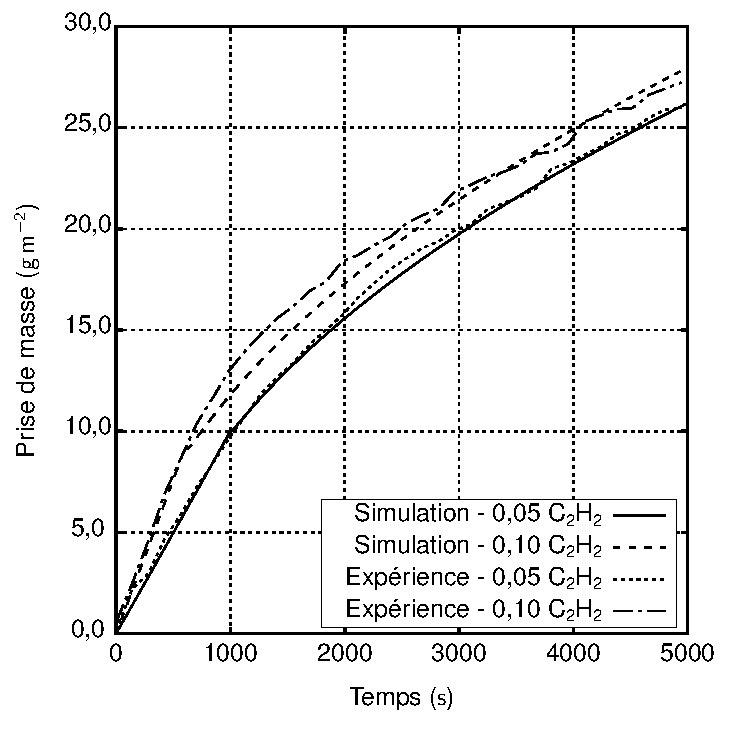
\includegraphics{figures/ch-03-mass_intake_hydrocarbon}}
  
  \caption{\label{fig:mass_intake_hydrocarbon}Comparaison des prises de masse en carbone à partir des hydrocarbures avec des simulations de l'équation de diffusion en utilisant le coefficient de diffusion fourni par \citet{Slycke1981ii} pour des alliages \ch{Fe-C} contenant des fractions en carbone équivalentes à la nuance 23MnCrMo5.}
\end{figure}

Pour ajuster les données nécessaires au modèle de diffusion, il faut supposer pendant cette période transitoire un flux en surface $J=\SI{5,6e-3}{\micro\mole\per\square\metre\per\second}$ pour 0,5\% de \ch{C2H2} à l'entrée ($J=\SI{8,5e-3}{\micro\mole\per\square\metre\per\second}$ pour 1,0\% de \ch{C2H2}). Pour satisfaire le comportement cinétique observé, selon la loi d'action de masse, il est normal que l'atmosphère contenant 0,5\% de \ch{C2H2} au départ produise un flux supérieur de 50\% à celui de l'atmosphère avec 1,0\% de \ch{C2H2} à l'entrée \textemdash{} celle plus riche en \ch{C2H2} ayant un avancement de décomposition homogène proportionnellement plus important. %Ces flux sont supérieurs à ceux produits par les taux de réaction proposés par \citet{Yada2013}, ce qui est lié au fait qu'il s'agit d'un alliage dont la diffusion a lieu en domaine multi-phasé et où la formation de cémentite ne représente pas la limite maximale d'enrichissement. 
Finalement une condition aux limites contrôlée par le transport en phase gazeuse s'établit, pour laquelle on calcule une constante de transfert de matière~\cite{Dulcy2007} $h\sim$~\SIlist{3;10}{\micro\mole\per\square\metre\per\second} correspondant aux deux atmosphères et une concentration en surface de l'ordre de 1,25-1,30\% en poids. Cette condition nécessaire pour expliquer les prises de masse mesurées implique la précipitation de cémentite pendant ces phases d'enrichissements. Le Tableau~\ref{tab:conditions-limite-pa} rassemble les expressions des flux utilisées dans les simulations des prises de masse pendant la période transitoire (flux constant) et à flux variable. Des pressions partielles de \ch{C2H2} de l'ordre de \SI{3}{\hecto\pascal} correspondant aux fractions en acétylène mesurées à la sortie du réacteur, lesquelles sont largement en dessous de celles à l'entrée, conduisent déjà à une condition de saturation en carbone à la surface des échantillons traités. %Selon \citet{Yada2013}, des pressions de l'ordre de 10\% de cette valeur seraient déjà suffisantes.

\begin{table}[h]
  \caption{\label{tab:conditions-limite-pa}Conditions aux limites pour la simulation de la prise de masse lors de la cémentation à pression atmosphérique. $C_{s}$ désigne la fraction molaire de carbone en surface.}
  
  \footnotesize{}\centering{}
  \begin{tabular}{\$l^l^l}
    \toprule[2pt]
    \multicolumn{1}{c}{\bfseries Type de condition}
    & \multicolumn{1}{c}{\bfseries 0,5\%~\ch{C2H2}}
    & \multicolumn{1}{c}{\bfseries 1,0\%~\ch{C2H2}}
    \tabularnewline
    \midrule[2pt]
    Flux constant 
    & $J=\SI{5,6e-3}{\micro\mole\per\square\metre\per\second}$ 
    & $J=\SI{8,5e-3}{\micro\mole\per\square\metre\per\second}$
    \tabularnewline
    Flux variable 
    & $J={3}\times(0,056-C_{s})~\si{\micro\mole\per\square\metre\per\second}$ 
    & $J={10}\times(0,057-C_{s})~\si{\micro\mole\per\square\metre\per\second}$
    \tabularnewline
    \bottomrule
  \end{tabular}
\end{table}

\subsubsection{Traitements à basse pression}

La cémentation de l'alliage 16NiCrMo13 a été réalisée sous une pression totale de \SI{50}{\hecto\pascal} à une température de \SI{1173}{\kelvin} avec les atmosphères et durées fournies Tableau~\ref{tab:cementation_bp}. Des débits de l'ordre de 2-3 fois supérieurs à ceux employés dans les études de pyrolyse ont pour but d'empêcher la décomposition homogène de \ch{C2H2} et donc de permettre l'arrivée du précurseur jusqu'à l'échantillon. Le résultat obtenu pour une atmosphère avec une pression partielle en \ch{C2H2} égale à \SI{2,5}{\hecto\pascal} suggère que la saturation en surface n'a pas été atteinte, ce qui se démarque des résultats à la pression atmosphérique si l'on considère que la pression partielle de \SI{3}{\hecto\pascal} mesurée dans les expériences à pression atmosphérique en sortie est responsable de l'enrichissement. Ceci n'est pas tout-à-fait vrai du fait de la décomposition de l'acétylène après contact avec l'échantillon. L'atmosphère carburante possède une pression partielle au moins supérieure à cette valeur à l'endroit où se trouve l'échantillon. Cela peut aussi être lié à la formation d'un dépôt carboné à pression atmosphérique \textendash{} observé sur les échantillons traités \textendash{} et à un contrôle cinétique à basse pression ne permettant pas d'atteindre la saturation en surface par des espèces carbonées.

\begin{table}[h]
  \caption{\label{tab:cementation_bp}Cémentation basse pression de l'alliage 16NiCrMo13.}
  
  \centering\footnotesize{}%
  \begin{tabular}{\$c^c^c^c^c^c}
    \toprule[2pt]
    \rowstyle{\bfseries}
    Atmosphère 
    & Débit 
    & Pression \ch{C2H2} 
    & Durée 
    & Surface traitée 
    & Gain de masse
    \tabularnewline
    \midrule[2pt]
    %
    \ch{N2 - 0,05 C2H2} 
    & \SI{636}{\sccm} 
    & \SI{2,5}{\hecto\pascal} 
    & \SI{3}{\hour} 
    & $8,80\times10^{-4}\,$\si{\square\metre} 
    & \SI{11,3}{\gram\per\square\metre}
    \tabularnewline
    %
    \ch{N2 - 0,25 C2H2} 
    & \SI{400}{\sccm} 
    & \SI{12,5}{\hecto\pascal} 
    & \SI{2}{\hour} & $8,80\times10^{-4}\,$\si{\square\metre} 
    & \SI{43,8}{\gram\per\square\metre}
    \tabularnewline
    \bottomrule
  \end{tabular}
\end{table}

Si l'on augmente la pression partielle de \ch{C2H2} à \SI{12,5}{\hecto\pascal} tout en réduisant le débit total à \SI{400}{\sccm}, la saturation en carbone à la surface est à nouveau atteinte et un fort enrichissement est observé. Ce résultat peut indiquer que la réaction de cémentation est composée \begin{inparaenum}[(i)] \item d'une réaction de craquage de \ch{C2H2} avec production de radicaux, ce qui peut se produire en surface comme dans le gaz et \item d'un apport de matière au solide. \end{inparaenum} En augmentant le débit, on limite la ré-absorption des radicaux et donc on reduit la réaction de cémentation. Alternativement, on peut supposer que le débit plus élevé empêche la formation d'un dépôt carboné pouvant assurer un enrichissement à concentration constante, ce qui représenterait une autre explication hydrodynamique au phénomène observé.

\section{Procédés utilisant de l'ammoniac}
\label{sec:pyrolyse_ammonia}

Les nitrurations gazeuses réalisées dans cette étude ont lieu sous des atmosphères à base d'ammoniac comme cela est présenté Tableau~\ref{tab:treatment_atmospheres} pour les traitements à la pression atmosphérique. Comme \ch{NH3} est très instable à \SI{1173}{\kelvin} \textendash{} température choisie pour les enrichissements \textendash{} l'équilibre entre la fraction résiduelle d'ammoniac à cette température et l'azote dans le matériau est utilisé pour le contrôle de l'atmosphère.  Thermo-Calc~\cite{Andersson2002,Borgenstam2000} permet de relier l'activité de l'azote dans le matériau à celle dans le gaz, permettant ainsi de généraliser la définition de potentiel nitrurant. La mise au point de l'atmosphère pour la nitruration se fait donc à partir des mesures de l'ammoniac résiduel dans le réacteur non-chargé et du calcul du potentiel de nitruration $K_{N}$ pour chaque alliage \textemdash{} voir Annexe~\ref{an:nitriding-kn}.

\subsection{Décomposition à la pression atmosphérique}

Le suivi de la décomposition de l'ammoniac à pression atmosphérique a été réalisé dans la plage de températures comprises entre \SIlist{773;1223}{\kelvin} en utilisant la chromatographie en phase gazeuse \textendash{} détecteur du type TCD \textendash{} pour la mesure de l'ammoniac résiduel. Les conditions expérimentales sont résumées Tableau~\ref{tab:decomposition-conditions-pa}.

\begin{table}[h]
  \caption{\label{tab:decomposition-conditions-pa}Conditions expérimentales pour l'étude de la décomposition de \ch{NH3} à pression atmosphérique dans le réacteur présenté Figure~\ref{fig:reacteur_pa}.}
  
  \footnotesize{}\centering{}
  \begin{tabular}{\$c^c^c^c^c}
    \toprule[2pt]
    \rowstyle{\bfseries}
    Température 
    & Débit 
    & Mélange 
    & Pression totale 
    & Pression \ch{NH3}
    \tabularnewline
    \midrule[2pt]
    \SIrange{773}{1223}{\kelvin}
    & \SI{415}{\sccm}
    & \ch{0,24 N2 - 0,72 H2 - 0,04 NH3}
    & \SI{1000}{\hecto\pascal}
    & \SI{40}{\hecto\pascal}
    \tabularnewline
    \bottomrule
  \end{tabular}
\end{table}

Les résultats (Figure~\ref{fig:ammonia_decomposition}) du suivi de la décomposition de l'ammoniac à la pression atmosphérique dans le réacteur en alumine décrit Section~\ref{sec:experimental_system} montrent un palier de conversion de l'ammoniac en dessous de \SI{900}{\kelvin} avec un taux de conversion $\alpha$ de l'ordre de 10\%. La faible vitesse de décomposition de l'ammoniac est connue depuis longtemps~\cite{Christiansen1935} et même en considérant l'effet de décomposition hétérogène sur les parois d'un réacteur en quartz~\cite{Cooper1988,Dirtu2006}, l'avancement de la réaction n'est pas très rapide. C'est à partir de ce comportement qu'un contrôle à l'état stationnaire du procédé est possible, donc à partir du débit~\cite{Gantois2010}. Lorsque l'atmosphère (Tableau~\ref{tab:treatment_atmospheres}) est composée d'un mélange ammoniac/ammoniac-craqué, le taux de conversion $\alpha$ de l'ammoniac doit être calculé en tenant compte du changement de volume apporté par la réaction globale de décomposition \ch{NH3 <=> 1/2 N2 + 3/2 H2}. La procédure généralisée présentée dans l'Annexe~\ref{an:ammonia_decomposition} est utilisée.

À partir de ce palier à \SI{900}{\kelvin}, \ch{NH3} devient très instable et la conversion augmente rapidement avec la température de la zone chaude du réacteur, pour atteindre 90\% à une température de \SI{1223}{\kelvin}. À \SI{1173}{\kelvin}, température adoptée pour les traitements thermochimiques dans ce travail, une fraction molaire résiduelle d'ammoniac égale à $5,5\times10^{-3}$ a été mesurée pour les conditions opératoires décrites. Après correction de la fraction molaire en dihydrogène issu de l'ammoniac décomposé, on trouve un potentiel nitrurant $K_{N}=\SI{8,6e-03}{\atm^{-0,5}}$.  D'après les diagrammes présentés Figure~\ref{fig:diagrammes_kn}, le traitement devrait produire des fractions massiques en azote atomique sur les surfaces traitées de l'ordre de 0,009 pour l'alliage 16NiCrMo13 et 0,010 pour la nuance 23MnCrMo5. Des résistances de transfert de matière à l'interface, liées à la composition des nuances traitées, peuvent limiter l'enrichissement.  Physiquement, ceci est lié au fait que les surfaces métalliques traitées catalysent le craquage du précurseur de nitruration et donc seule une faible fraction des molécules de \ch{NH3} adsorbées sur le métal apporte effectivement~\cite{Wrobel2006,Arabczyk2009} de l'azote à l'alliage. Dans le cas plus général des réacteurs industriels, les structures constituant le four sont à considérer.

\subsection{Décomposition sous pression réduite}
\label{sec:decomposition_nh3_bp}

Aux températures employées dans les traitements en phase austénitique des matériaux, l'ammoniac devrait être presque complètement dissocié. Ceci a été mis en évidence à la pression atmosphérique. Ce n'est toutefois pas le cas à basse pression pour des débits similaires. Cela est le résultat de l'augmentation de la vitesse moyenne du gaz qui évolue à l'inverse de la pression de travail. En utilisant une atmosphère composée de \ch{N2 - 0,25 NH3} à \SI{50}{\hecto\pascal} sous un débit total de \SI{684}{\sccm} aucune décomposition mesurable n'est observée dans la zone chaude du réacteur \textemdash{} de \SIrange{473}{1173}{\kelvin}.  Pour vérifier comment agit la loi d'action de masse, nous avons utilisé une atmosphère \ch{N2 - 0,64 NH3} sous un débit \SI{737}{\sccm} une fois à une pression de \SI{50}{\hecto\pascal} et à \SI{1173}{\kelvin} et une fois à une pression de \SI{100}{\hecto\pascal} et à \SI{1223}{\kelvin}. Aucune décomposition n'a été détectée et ces conditions ont été choisies pour la nitruration. Le Tableau~\ref{tab:decomposition-conditions-bp} rassemble ces conditions. 

\begin{table}[!h]
  \caption{\label{tab:decomposition-conditions-bp}Conditions expérimentales pour l'étude de la décomposition du \ch{NH3} à basse pression dans le réacteur présenté Figure~\ref{fig:reacteur_bp}.}
  
  \footnotesize{}\centering{}
  \begin{tabular}{\$c^c^c^c^c}
    \toprule[2pt]
    \rowstyle{\bfseries}
    Température 
    & Débit 
    & Mélange 
    & Pression totale 
    & Pression \ch{NH3}
    \tabularnewline
    \midrule[2pt]
    \SIrange{473}{1173}{\kelvin}
    & \SI{684}{\sccm}
    & \ch{0,75 N2 - 0,25 NH3}
    & \SI{50}{\hecto\pascal}
    & \SI{12,5}{\hecto\pascal}
    \tabularnewline
    %
    \SI{1173}{\kelvin}
    & \SI{737}{\sccm}
    & \ch{0,36 N2 - 0,64 NH3}
    & \SIlist{50;100}{\hecto\pascal}
    & \SIlist{32;64}{\hecto\pascal}    
    \tabularnewline
    %
    \SIrange{773}{1173}{\kelvin}
    & \SI{470}{\sccm}
    & \ch{NH3}
    & \SIlist{50;100}{\hecto\pascal}
    & \SIlist{50;100}{\hecto\pascal}         
    \tabularnewline  
    \bottomrule
  \end{tabular}
\end{table}

En réduisant le débit à \SI{470}{\sccm} et en utilisant une atmosphère composée d'ammoniac pur, on mesure un faible taux de décomposition qui conduit à la formation d'une fraction de moins de 0,04 en diazote. Cette décomposition est liée au temps de séjour plus important dans la zone chaude du réacteur et est légèrement plus prononcée à \SI{100}{\hecto\pascal} qu'à \SI{50}{\hecto\pascal}, comme attendu.  La Figure~\ref{fig:ammoniac_bp} présente l'ammoniac résiduel en fonction de la température de la zone chaude du réacteur. La fin du palier de stabilité de l'ammoniac est cohérent avec les résultats à la pression atmosphérique (Figure~\ref{fig:ammonia_decomposition}). Seul l'ammoniac et le diazote ont été séparés par les colonnes du chromatographe.

\begin{figure}[h]
  \centering
  \subfloat[\label{fig:ammonia_decomposition}Pression atmosphérique.]{
    \centering\resizebox{0.98\textwidth}{!}{
    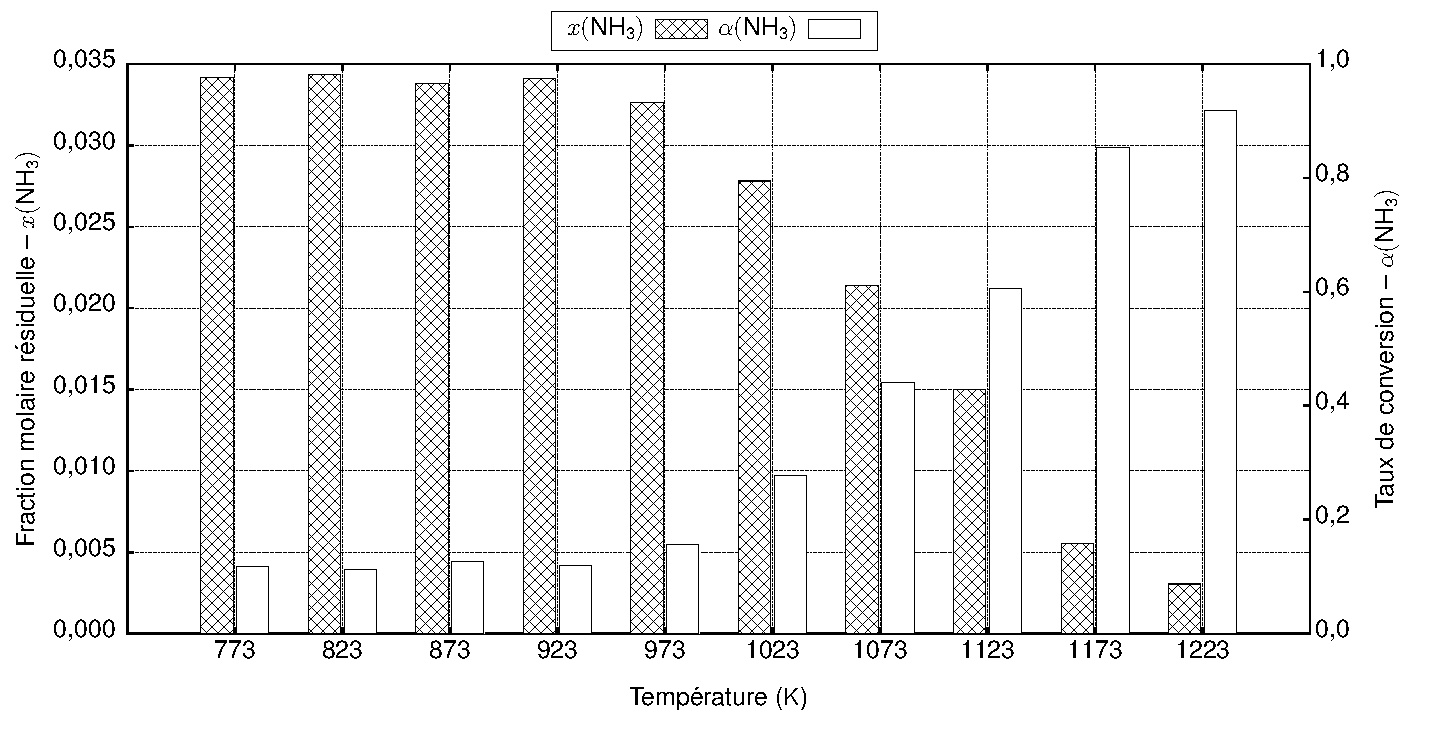
\includegraphics{figures/ch-03-decomposition_nh3_pa}}
  }\\
  \subfloat[\label{fig:ammoniac_bp}Basse pression.]{
    \centering\resizebox{0.98\textwidth}{!}{
    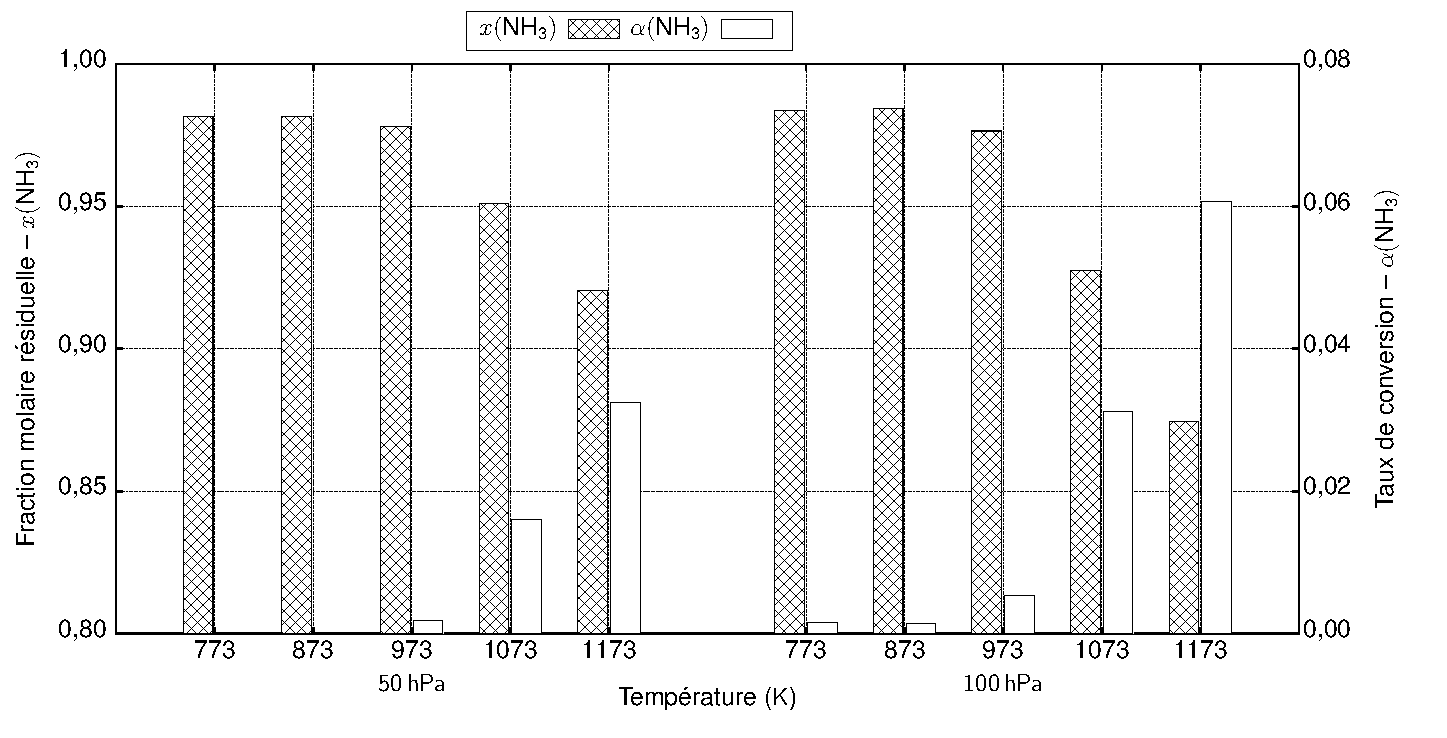
\includegraphics{figures/ch-03-decomposition_nh3_bp}}
  }

  \caption{\label{fig:ammoniac_residuel}Ammoniac résiduel et taux de conversion en fonction de la température de la zone chaude du réacteur: résultats \protect\subref{fig:ammonia_decomposition} à pression atmosphérique et \protect\subref{fig:ammoniac_bp} basse pression.}
\end{figure}

\subsection{Nitruration sous pression réduite}
\label{sec:nitruration-ammoniac}

La nitruration austénitique à basse pression de l'alliage 16NiCrMo13 a été conduite à \SI{1173}{\kelvin} sous une pression de \SI{50}{\hecto\pascal} pendant \SI{3}{\hour}. Ce traitement a été réalisé sous une atmosphère \ch{N2 - 0,64 NH3} avec un débit total de \SI{737}{\sccm} et sous une atmosphère \ch{N2 - 0,23 NH3} sous un débit total de \SI{682}{\sccm}.  Ces conditions ont été choisies en fonction des résultats de la Section~\ref{sec:decomposition_nh3_bp} où il a été montré qu'aucune décomposition de l'ammoniac n'est détectée dans la limite de précision de nos mesures. Le Tableau~\ref{tab:nitruration_bp} présente les traitements réalisés avec les surfaces métalliques exposées et les gains de masse respectifs des échantillons.

\begin{table}[h]
  \caption{\label{tab:nitruration_bp}Nitruration austénitique de l'alliage 16NiCrMo13.}
  
  \centering\footnotesize{}
  \begin{tabular}{\$c^c^c^c}
    \toprule[2pt]
    \rowstyle{\bfseries}
    Atmosphère 
    & Débit 
    & Surface traitée 
    & Gain de masse
    \tabularnewline
    \midrule[2pt] 
    \multirow{2}{*}{\ch{N2 - 0,64 NH3}} 
    & \multirow{2}{*}{\SI{737}{\sccm}} 
    & \SI{1,81e-3}{\square\metre} 
    & \SI{13,1}{\gram\per\square\metre}
    \tabularnewline
    %\cmidrule{3-4} 
    &  
    & \SI{9,54e-4}{\square\metre} 
    & \SI{18,5}{\gram\per\square\metre}
    \tabularnewline
    %
    \ch{N2 - 0,23 NH3} 
    & \SI{682}{\sccm} 
    & \SI{8,80e-4}{\square\metre} 
    & \SI{9,3}{\gram\per\square\metre}
    \tabularnewline
    \bottomrule
  \end{tabular}
\end{table}

On observe un gain de masse par unité de surface plus important pour la condition la plus riche en ammoniac.  En revanche, l'atmosphère contenant une fraction en ammoniac de 0,64 conduit à un enrichissement plus important si le réacteur est moins chargé. Le chargement de \SI{1,81e-3}{\square\metre} correspond à deux échantillons de dimensions équivalentes de \SI{9,54e-4}{\square\metre} placés côté-à-côté dans la même section transversale du réacteur: le taux de craquage en surface est plus prononcé dans la condition où la surface exposée est plus importante \textemdash{} le nombre de moles du système augmente plus rapidement, ce qui entraîne une accélération plus prononcée du mélange et donc un temps de séjour plus court. L'enrichissement est donc moins prononcé, même si l'atmosphère de départ est constante et que le flux de \ch{NH3} en phase gazeuse est largement supérieur à celui requis pour enrichir le solide. En raison de cette hétérogénéité, l'obtention d'une constante cinétique ne peut pas être directe. 

La Figure~\ref{fig:bilan_matiere_nitruration_bp} présente le bilan des espèces mesurées par chromatographie gazeuse pendant les traitements. On vérifie que les fractions en \ch{NH3} en sortie à l'état stationnaire \textendash{} fin de traitement \textendash{} pour l'atmosphère \ch{N2 - 0,64 NH3} sont indépendantes de la surface exposée. Ce n'est possible que si l'hypothèse de changement de temps de séjour \textendash{} ici il vaudrait mieux parler de \og{}temps de contact\fg{} \textendash{} proposée pour expliquer l'enrichissement est valable, ou que \ch{NH3} est formé après contact avec l'échantillon par récombinaison de ses produits de déshydrogénation partielle, via des processus du type \ch{NH + H <=> NH2} et \ch{NH2 + H <=> NH3}. 

Il faut aussi remarquer sur la Figure~\ref{fig:bilan_matiere_nitruration_bp} que la pente de la fraction molaire de \ch{NH3} au cours du traitement est plus élevée pour la condition la moins chargée (surface exposée moins importante), ce qui indique l'établissement d'un état stationnaire plus rapide et confirme les observations précédentes. Cela implique que pour des applications industrielles à basse pression, le diagnostic de la phase gazeuse pour la mise au point de traitements dépendra du chargement \textendash{} et naturellement de l'état de surface des pièces \textendash{} ainsi que du débit et donc pas seulement de l'ammoniac résiduel en équilibre avec les surfaces. Ce n'est qu'après l'établissement de l'état stationnaire qu'une condition aux limites de type concentration constante est possible. De cette manière l'enrichissement se fait globalement avec une condition transitoire sur les surfaces.

\vfill
\begin{figure}[!ht]
  \centering\noindent
  \begin{tikzpicture}
   \node at (0.0,+0.0) {
     \centering\noindent
     \begin{tikzpicture}%
     \node[anchor=south west,inner sep=0] (A) at (0,0) {%
       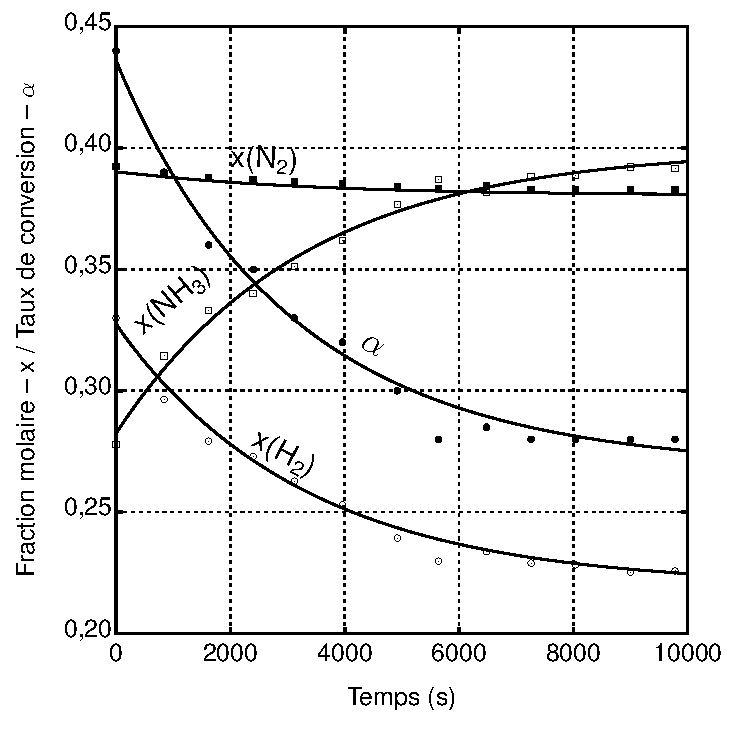
\includegraphics[width=7.5cm]
       {figures/ch-03-nitriding_balance_bp_experiment_1}
     };
     \begin{scope}[x={(A.south east)},y={(A.north west)}]
       \node at (0.55,1.0) 
       {\footnotesize\ch{N2 - 0,64 NH3} - S~=~\SI{1,81e-3}{\square\metre}};
     \end{scope}
     \end{tikzpicture}
   };
   \node at (8.0,+0.0) {
     \centering\noindent
      \begin{tikzpicture}%
      \node[anchor=south west,inner sep=0] (A) at (0,0) {%
        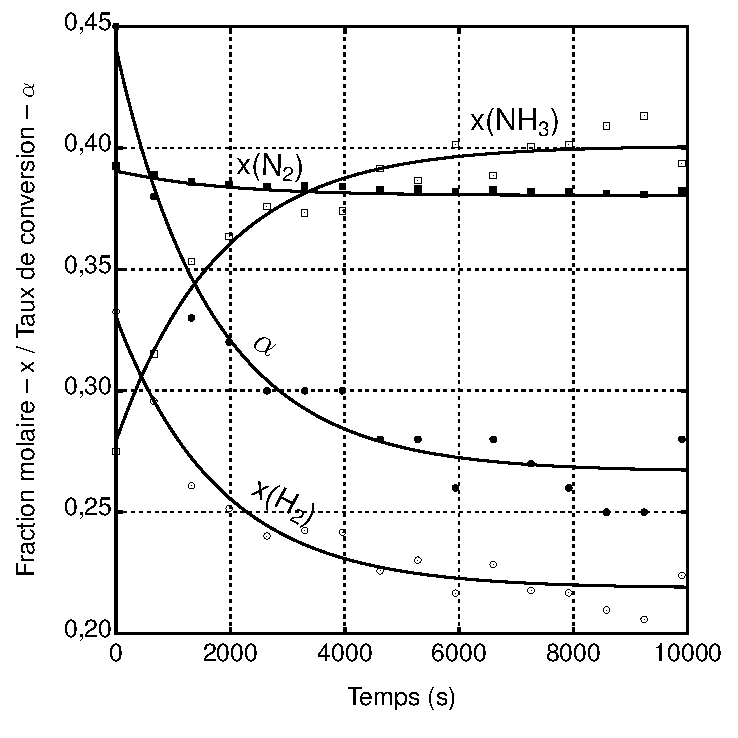
\includegraphics[width=7.5cm]
        {figures/ch-03-nitriding_balance_bp_experiment_2}
      };
      \begin{scope}[x={(A.south east)},y={(A.north west)}]
      \node at (0.55,1.0) 
      {\footnotesize\ch{N2 - 0,64 NH3} - S~=~\SI{9,54e-4}{\square\metre}};
      \end{scope}
      \end{tikzpicture}
   };
   \node at (4.0,-8.0) {
     \centering\noindent
      \begin{tikzpicture}%
      \node[anchor=south west,inner sep=0] (A) at (0,0) {%
        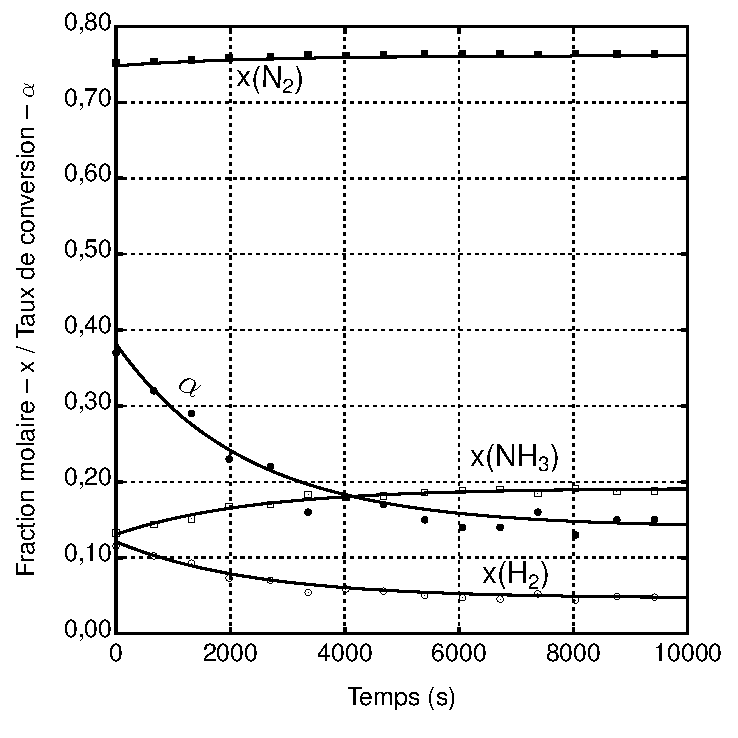
\includegraphics[width=7.5cm]
        {figures/ch-03-nitriding_balance_bp_experiment_3}
      };
      \begin{scope}[x={(A.south east)},y={(A.north west)}]
      \node at (0.55,1.0) 
      {\footnotesize\ch{N2 - 0,23 NH3} - S~=~\SI{8,80e-4}{\square\metre}};
      \end{scope}
      \end{tikzpicture}
   };
  \end{tikzpicture}

  \caption{\label{fig:bilan_matiere_nitruration_bp}Bilan matière de la nitruration austénitique: évolution des fractions molaires des espèces à la sortie du réacteur pour les traitements réalisés en utilisant des atmosphères \ch{N2 - 0,64 NH3}. Les données pour \ch{NH3} et \ch{N2} sont issues des mesures, tandis que pour \ch{H2} elles ont été calculées.}
\end{figure}
\vfill

\clearpage\section{Conclusion}

Cette section concerne les résultats expérimentaux présentés Chapitre~\ref{ch:caracterisation_atmospheres} sur la mise au point des atmosphères utilisées dans les traitements thermochimiques. Ce chapitre peut se résumer ainsi:
\begin{itemize}
  \item les études ont été réalisées dans des réacteurs tubulaires à pression atmosphérique et à basse pression; le transport des espèces dans le réacteur à pression atmosphérique a été caractérisé en utilisant la méthode du pulse d'un traceur; un système d'échantillonnage à basse pression a été présenté pour les études de décomposition des précurseurs;
  
  \item la température de point de rosée de l'atmosphère employée pour la cémentation des alliages a été calculée en fonction de la teneur en carbone visée sur les surfaces; ces résultats se trouvent être en bon accord avec les méthodes classiques;
  
  \item la pyrolyse de l'acétylène a été étudiée à pression atmosphérique et à basse pression; dans les deux cas on a suivi les hydrocarbures de types $C_{1}$ et $C_{2}$; pour les temps de séjour mesurés du réacteur à pression atmosphérique, l'avancement de la réaction de pyrolyse dépasse les 75\% et le bilan matière montre que des espèces et radicaux fortement carbonés sont présents en sortie du réacteur; cependant, à basse pression, le taux de décomposition n'est que de 20\% à \SI{30}{\hecto\pascal} et de 60\% à \SI{100}{\hecto\pascal} à partir d'un mélange \ch{N2 - 0,36 C2H2};
  
  \item à partir de la décomposition de l'ammoniac à la pression atmosphérique on a établi la condition aux limites d'enrichissement pour les simulations de diffusion de l'azote dans le matériaux; contrairement à la thermodynamique de la réaction globale de décomposition de \ch{NH3}, de très faibles niveaux de conversion ont été mesurés à basse pression même à \SI{1173}{\kelvin}, ce qui a été attribué à l'effet cinétique d'action de masse dans le système;
  
  \item la cémentation à partir des hydrocarbures permet l'enrichissement même au--delà de la saturation en surface et les résultats suggèrent un mécanisme de craquage suivie d'une adsorption conduisant à l'enrichissement au lieu d'un enrichissement direct par craquage des hydrocarbures en surface;
  
  \item des résultats similaires ont été obtenus pour la nitruration en domaine austénitique. La variation de surface de la charge du réacteur, qui conduit à des résultats similaires en concentration à la sortie des produits formés permet d'inférer que la recombinaison des produits de décomposition conduit à reformer en partie \ch{NH3} en phase gazeuse. 
\end{itemize}

\endinput
  \cleardoublepage\chapter{Réponses métallurgiques}
\label{ch:reponse_metallurgique}

\vfill

Les propriétés d'usage d'un matériau dépendent du procédé mis en {\oe}uvre lors de l'élaboration et donc des microstructures qui en résultent, celles-ci étant liées essentiellement à la composition du matériau utilisé. Les paramètres de contrôle des enrichissements en carbone et en azote des alliages à base de fer et plus spécifiquement des nuances 16NiCrMo13 et 23MnCrMo5 ayant déjà été définis et présentés dans les chapitres précédents, ce chapitre décrit plus particulièrement les études expérimentales réalisées en carbonitruration et les résultats obtenus sur les propriétés mécaniques et les microstructures formées. Cette partie s'appuiera donc sur les informations relatives aux gammes de cémentation et de nitruration qui ont été mises au point Chapitre~\ref{ch:caracterisation_atmospheres}. Les résultats obtenus sur les deux alliages étudiés suite aux traitements effectués selon les modalités décrites Section~\ref{sec:methodes_metallurgie} sont présentés Section~\ref{sec:comparaison_procedes} sous forme de profils de diffusion des éléments interstitiels. Ces résultats sont confrontés à des simulations conduites avec Thermo-Calc~\cite{Andersson2002,Borgenstam2000} et avec la méthode simplifiée décrite Section~\ref{sec:integration_slycke}. La Section~\ref{sec:reponses_mecaniques} présente les propriétés mécaniques établies à partir des filiations de dureté puis les microstructures obtenues sont discutées Section~\ref{sec:precipitation}, à partir des études réalisées en microscopie électronique en transmission. Elles permettent l'identification des précipités formés lors des différents traitements et, donc, de proposer un mécanisme à l'origine de l'amélioration de la tenue en dureté qui est observée lors du revenu après carbonitruration plutôt qu'après cémentation. Le lien entre compositions locales et réponses métallurgiques sera alors établi et comprend les relations entre dureté, microstructure et composition. Ce chapitre a donné lieu a une publication et il est partiellement présenté sur \citet{DalMaz2017}.

\vfill\clearpage

\section{Méthodes expérimentales}
\label{sec:methodes_metallurgie}

\subsection{Paramètres de traitement employés}
\label{sec:parametres_traitement}

L'étude des réponses mécaniques et métallurgiques aux traitements de carbonitruration, de cémentation et de nitruration austénitique des alliages étudiés (Tableau~\ref{tab:composition_alliages}), a été réalisée à la pression atmosphérique pour une température fixe d'enrichissement et de diffusion de \SI{1173}{\kelvin} en employant le réacteur tubulaire vertical présenté Figure~\ref{fig:reacteur_pa}. La température a été choisie au milieu de la plage typiquement employée dans les traitements thermochimiques et représente une limite pratique pour traiter les nuances qui n'ont pas été élaborées avec des éléments stabilisant la taille de grain austénitique~\cite{Yang2013}. De cette manière, toutes les microstructures qui seront comparées sont issues d'une condition unique de trempe après enrichissement. Pour les étapes d'enrichissement en carbone et en azote, les atmosphères \ch{N2 - 0,2 CO - 0,4 H2} et \ch{N2 - 0,72 H2 - 0,04 NH3} du Tableau~\ref{tab:treatment_atmospheres} ont été utilisées, respectivement. Le chauffage du réacteur chargé avec un échantillon a été réalisé sous atmosphère inerte composée de \ch{N2 - 0,2 H2} en fraction volumique avec un débit total de \SI{500}{\sccm} pendant une durée d'environ \SI{3}{\hour} pour atteindre la température d'enrichissement. Ces conditions sont résumées Tableau~\ref{tab:conditions-traitement}.
% et correspondent aux différentes étapes de traitement définies aux Sections~\ref{sec:classical_carburizing}~et~\ref{sec:pyrolyse_ammonia}.

\begin{table}[h]
  \caption{\label{tab:conditions-traitement}Conditions de traitement et aux limites pour les étapes de cémentation, nitruration et diffusion des différents cycles de traitements thermochimiques réalisés.}
  
  \centering{}\footnotesize{}
  \begin{tabular}{\$l^c^c^l^l}
    \toprule[2pt]
    \multicolumn{1}{c}{\bfseries Étape}
    & \multicolumn{1}{c}{\bfseries Température}
    & \multicolumn{1}{c}{\bfseries Pression}
    & \multicolumn{1}{c}{\bfseries Atmosphère}
    & \multicolumn{1}{c}{\bfseries Condition aux limites}
    \tabularnewline
    \midrule[2pt]
    Cémentation 
    & \multirow{3}{2cm}[-6pt]{\centering\SI{1173}{\kelvin}}
    & \multirow{3}{2cm}[-6pt]{\centering\SI{1000}{\hecto\pascal}}
    & \ch{N2 - 0,2 CO - 0,4 H2}
    & $T_{r}=\SI{263}{\kelvin}$
    %
    \tabularnewline[6pt]
    Nitruration & &
    & \ch{N2 - 0,72 H2 - 0,04 NH3} 
    & $K_{N}=\SI{8,6e-03}{\atm^{-0,5}}$
    %
    \tabularnewline[6pt]
    Diffusion & &
    & \ch{N2 - 0,2 H2}
    & Flux nul
    \tabularnewline
    \bottomrule
  \end{tabular}
\end{table}

Les enrichissements en carbone, soit pour la carbonitruration soit pour la cémentation, ont été réalisés pendant \SI{2}{\hour}. Dans le cas de la nitruration et de la carbonitruration, les enrichissements en azote ont été effectués pendant \SI{3}{\hour}. Après l'enrichissement en carbone de l'alliage 16NiCrMo13, une étape de diffusion à flux nul de \SI{1}{\hour} a été imposée avant la nitruration, ce qui constitue le traitement de carbonitruration. Pour obtenir un profil en carbone similaire, il a fallu faire suivre la cémentation de l'alliage 16NiCrMo13 d'une étape de diffusion à flux nul de \SI{4}{\hour}. Dans le cas de l'alliage 23MnCrMo5, l'étape d'enrichissement en carbone due à la carbonitruration a été suivie directement par la nitruration, ce qui implique de devoir imposer une étape de diffusion à flux nul de \SI{3}{\hour} après enrichissement en carbone pour le traitement de cémentation. La nitruration des deux alliages a lieu en une seule étape d'enrichissement de \SI{3}{\hour}. Un résumé de ces conditions se trouve présenté Tableau~\ref{tab:treatment-conditions} et représenté sur la Figure~\ref{fig:heat-cycles}. En outre, quelques échantillons ont été trempés directement après l'enrichissement en carbone pour obtenir la réponse mécanique correspondant à de fortes teneurs en carbone. Cela a permis d'alimenter le modèle de durcissement au--delà du point--H~\cite{Sherby2008}.

\begin{table}[h]
  \begin{minipage}{\textwidth} 
    \renewcommand*\footnoterule{}
    \caption{\label{tab:treatment-conditions}Durées des étapes d'enrichissement des traitements de cémentation, de nitruration, de carbonitruration et des revenus réalisés. Les champs remplis avec un tiret indiquent que l'étape d'enrichissement/diffusion ne fait pas partie du traitement.}
    
    \centering{}\footnotesize{}
    \begin{tabular*}{\textwidth}{@{\extracolsep{\fill}}llcccc} 
      \toprule[2pt]
      % line 1
      \multirow{2}{*}[-3pt]{\centering\bfseries Traitement} &
      \multirow{2}{*}[-3pt]{\centering\bfseries Alliage} &
      \multicolumn{3}{c}{\bfseries 
        Durée d'enrichissement/diffusion à \SI{1173}{\kelvin}} &
      \multirow{2}{*}[-6pt]{\parbox{1.5cm}{
          \centering\bfseries Revenu~\footnote{
            Les échantillons nitrurés ont subi un revenu pendant \SI{18}{\hour} à \SI{673}{\kelvin}.} (\ch{N2-H2})}}\\
      %line 2
      \cmidrule(l){3-5} & 
      ~ & 
      \multicolumn{1}{p{2cm}}{\centering\bfseries Carbone \\ (\ch{CO-H2-N2})} &
      \multicolumn{1}{p{2cm}}{\centering\bfseries Diffusion \\ (\ch{N2-H2})} &
      \multicolumn{1}{p{2cm}}{\centering\bfseries Azote \\ (\ch{NH3-H2-N2})}\\
      \midrule[2pt]
      %line 3
      \multirow{2}{*}[-3pt]{Cémentation} & 16NiCrMo13 &
      \multirow{2}{*}[-0pt]{\SI{2}{\hour}} & \SI{4}{\hour} &
      \multirow{2}{*}[-0pt]{-} & 
      \multirow{5}{*}[-6pt]{
        \parbox{1.5cm}{\centering 
          \SI{70}{\hour} à \SI{453}{\kelvin}   \\[9pt]
          \SI{18}{\hour} à \SI{573}{\kelvin} }}\\[3pt]
      %line 4
      & 23MnCrMo5 & ~ & \SI{3}{\hour} & &\\[6pt]
      %line 5
      \multirow{1}{*}[-0pt]{Nitruration} & tous les deux  & - & - &
      \multirow{1}{*}[-0pt]{\SI{3}{\hour}} &\\[6pt]
      %line 6	
      \multirow{2}{*}[-0pt]{Carbonitruration} & 16NiCrMo13 &
      \multirow{2}{*}[-0pt]{\SI{2}{\hour}} & \SI{1}{\hour} &
      \multirow{2}{*}[-0pt]{\SI{3}{\hour}} &\\[3pt]
      %line 7
      & 23MnCrMo5 & ~ & - & &\\ 
      \bottomrule 
    \end{tabular*}
  \end{minipage}
\end{table}

\begin{figure}[!h]
  \centering\resizebox{0.98\textwidth}{!}{
    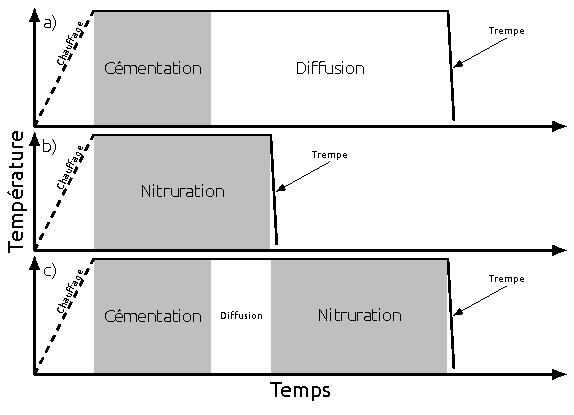
\includegraphics{figures/ch-04-heat_cycles}}
  
  \caption{\label{fig:heat-cycles}Représentation graphique des cycles thermiques des traitements d'enrichissement à \SI{1173}{\kelvin} définis dans le Tableau~\ref{tab:treatment-conditions}: a) cémentation, b) nitruration et c) carbonitruration. Les traitements de revenu ne sont pas représentés.}
\end{figure}

Finalement, pour atteindre les propriétés mécaniques envisagées, tous les traitements ont été suivis d'une trempe à l'huile à la température ambiante \textendash{} soit environ \SI{298}{\kelvin} \textendash{} et d'un traitement cryogénique dans l'azote liquide en ébullition \textendash{} à \SI{77}{\kelvin}. Après le traitement cryogénique, les échantillons ont été soumis à un revenu soit de \SI{18}{\hour} à \SI{573}{\kelvin}, soit de \SI{70}{\hour} heures à \SI{453}{\kelvin}. Le revenu à plus haute température doit permettre l'étude de la stabilité des couches dans des conditions sévères d'opération, alors que le revenu correspond à l'approche classiquement employée avec ce type de traitements thermochimiques. Dans le cas de la nitruration austénitique, un revenu pendant \SI{18}{\hour} à \SI{673}{\kelvin} a aussi été réalisé.

\subsection{Caractérisation des échantillons}
\label{sec:caracterisation_materiaux}

Les échantillons traités dans les conditions décrites à la section précédente pour l'étude des propriétés mécaniques et métallurgiques ont été caractérisés par microscopie optique (MO), microscopie électronique en transmission (MET) et micro-dureté Vickers (HV). Pour les analyses MO et HV, les échantillons ont été enrobés dans une résine époxy et préparés par polissage au papier abrasif jusqu'à une taille de particule inférieure à \SI{14}{\micro\metre}, étape qui a été suivie par un polissage au moyen d'une suspension en alumine jusqu'à une taille de particules inférieure à \SI{0,01}{\micro\metre}. Les indentations Vickers ont été réalisées avec une charge de \SI{300}{gf}. Les profils de diffusion ont été déterminés en employant une micro-sonde électronique Jeol-JXA-8530F. Une procédure similaire à celle qui vient d'être décrite a été adoptée pour la préparation des échantillons servant à la détermination des profils de diffusion mais dans ce cas la résine d'enrobage a été remplacée par un alliage métallique à bas point de fusion ($\approx\SI{353}{\kelvin}$) pour assurer une meilleure conductivité requise par les analyses. Les mesures ont été réalisées tous les \SI{25}{\micro\metre} et la quantification des résultats s'est faite selon la méthode d'étalonnage décrite par \citet{Catteau2014} (en utilisant du $\gamma^{\prime}$\ch{Fe4N} st{\oe}chiométrique pour l'azote et la méthode de la courbe de calibration proposée par \cite{Robaut2006} pour le carbone).

Dans le cas de la microscopie en transmission, réalisée sous un potentiel de \SI{200}{\kilo\volt}, les lames minces ont été prélevées à une distance fixe de \SI{100}{\micro\metre} de la surface traitée. Les lames ont été préparées par la technique FIB~\footnote{de l'anglais \textit{Focused Ion Beam}, Sonde Ionique Focalisée, voir \citet{Williams2009}.} et par polissage manuel des lames jusqu'à une épaisseur inférieure à \SI{50}{\micro\metre} suivi d'une attaque électrolytique. Le MET a été employé pour l'identification des précipités par microanalyse chimique qui permet l'établissement de cartographies de composition par EDX~\footnote{de l'anglais \textit{Energy Dispersive X-ray}, Analyse Dispersive en Énergie, voir \citet{Williams2009}.}. La spectrométrie de pertes d'énergie des électrons (EELS) a été employée comme moyen plus précis de localisation des éléments interstitiels. Les phases présentes ont été identifiées par diffraction des électrons.

\section{Profils de diffusion et prise de masse}
\label{sec:comparaison_procedes}

Les enrichissements réalisés ont été évalués par mesure de prises de masse et par détermination des profils de diffusion dans les échantillons. À partir de l'intégration des profils mesurés par micro-sonde, la prise de masse par unité de surface peut être estimée selon l'Équation~\ref{eq:mass_gain} (Annexe~\ref{an:integration_diffusion}). Les valeurs ainsi obtenues sont comparées à des simulations réalisées à l'aide de Thermo-Calc~\cite{Andersson2002,Borgenstam2000} et de l'intégration numérique du système simplifié \ch{Fe-C-N} décrit à la Section~\ref{sec:integration_slycke}. Bien que Thermo-Calc~\cite{Andersson2002,Borgenstam2000} prenne en compte la précipitation des nitrures et l'interaction entre les éléments interstitiels et la matrice, l'intérêt de l'approche simplifiée réside dans la possibilité d'une utilisation rapide dans un contexte industriel. L'effet d'interaction entre éléments interstitiels est bien connu~\cite{Bhadeshia1980,Bhadeshia2004,Oda1994,Sozinov1997225,Sozinov1999927} et il doit être pris en compte pour une prédiction fiable des profils de diffusion. On peut montrer, par exemple, que pour simuler une prise de masse intégrant l'équation de la diffusion avec un schéma de Crank-Nicolson~\cite{CrankNicolson1947} à concentration constante et égale à la saturation en surface, le coefficient de diffusion du carbone indépendant de la composition~\cite{Slycke1981ii} doit être multiplié par un facteur de 1,8--2,0 pour obtenir un résultat en accord avec les mesures~\cite{Bhadeshia2004}.

Cette analyse a pour but de vérifier la cohérence entre la méthode macroscopique \textendash{} mesure de variation de masse \textendash{} et microscopique \textendash{} micro-sonde \textendash{} et leur convergence selon les conditions aux limites employées dans les simulations. Plusieurs sources d'écart sont possibles entre ces approches: \begin{inparaenum}[(i)] \item le gain de masse par oxydation de surface, \item l'imprécision de la balance et la mesure de surface des pièces, \item l'état de préparation des surfaces, \item les effets de bord qui affectent l'homogénéité de l'enrichissement, \item l'effet de numéro atomique sur l'absorption des rayons x dans les mesures de sonde, \item l'imprécision des données thermodynamiques, etc. \end{inparaenum} Le Tableau~\ref{tab:mass_gain} présente une comparaison entre ces différentes sources de données pour les études réalisées. Les profils de diffusion mesurés sont présentés Figure~\ref{fig:diffusion_profiles}. Cependant, l'ordre de grandeur des valeurs \og{}mesurées\fg{} et simulées reste proche et l'analyse s'avère utile pour valider les conditions aux limites employées dans les simulations des profils de diffusion.

\begin{table}[h]
  \caption{\label{tab:mass_gain}Comparaison entre les prises de masse mesurées et simulées.}
  
  \footnotesize{}\centering{}
  \begin{tabular*}{\textwidth}{@{\extracolsep{\fill}}lcccc} 
    \toprule[2pt]
    % line 1
    \multirow{2}{*}[-3pt]{\centering\bfseries Traitement} &
    \multicolumn{4}{c}{\bfseries Prise de masse (\si{\gram\per\square\metre})}\\
    %line 2
    \cmidrule(l){2-5} & 
    \multicolumn{1}{p{2.5cm}}{
      \centering\bfseries Mesurée  \\ {\tiny{}(Balance)}} & 
    \multicolumn{1}{p{2.5cm}}{
      \centering\bfseries Intégrée \\ {\tiny{}(Micro-sonde)}} &
    \multicolumn{1}{p{2.5cm}}{
      \centering\bfseries Simulée  \\ {\tiny{}(Thermo-Calc)}} &
    \multicolumn{1}{p{2.5cm}}{
      \centering\bfseries Simulée  \\ {\tiny{}(Annexe~\ref{an:integration_diffusion})}} \\
    \midrule[2pt]
    \multicolumn{5}{c}{Alliage 16NiCrMo13}\\
    \midrule[1pt]
    %line 3
    Cémentation
    & 28,8 & 23,5 & 21,0 & 22,2 \\[6pt]
    %line 5
    Nitruration
    & 6,3 & 5,0 & 6,0 & - \\[6pt]
    %line 6	
    Carbonitruration
    & 22,1 & 21,0 & 22,2 & - \\
    \midrule[2pt]
    \multicolumn{5}{c}{Alliage 23MnCrMo5}\\  
    \midrule[1pt]
    %line 3
    Cémentation
    & 20,5 & 15,3 & 17,6 & 17,6 \\[6pt]
    %line 5
    Nitruration
    & 8,5 & 5,8 & 6,1 & - \\[6pt]
    %line 6	
    Carbonitruration
    & 29,0 & 25,1 & 29,1 & - \\
    \bottomrule 
  \end{tabular*}
\end{table}

\begin{table}[!hb]
	\caption{\label{tab:conditions-sim-diffusion}Conditions aux limites pour la simulation des profils de diffusion réalisées à l'aide de Thermo-Calc~\cite{Andersson2002,Borgenstam2000} et selon Annexe~\ref{an:integration_diffusion} pour les étapes de cémentation et nitruration des traitements thermochimiques. Les étapes de diffusion à flux nul ont été simulées en considérant le système fermé. Un flux $J_{i}$ (où $i=\ch{C},\ch{N}$) positif désigne l'entrée de l'élément dans le matériau. Les activités sont notées $a_{i}^{m}$ et les fractions massiques $w_{i}$.}
	
	\centering{}\footnotesize{}
	\begin{tabular}{lclc}
		\toprule[2pt]
		\multicolumn{1}{c}{\bfseries{}Étape}
		& \textbf{Alliage} 
		& \multicolumn{1}{c}{\bfseries{}Thermo-Calc~\cite{Andersson2002,Borgenstam2000}} 
		& \textbf{Annexe}~\ref{an:integration_diffusion}
		\tabularnewline
		\midrule[2pt]
		\multirow{2}{2cm}[-3pt]{Cémentation}
		& 16NiCrMo13 & $a_{\ch{C}}^{m}=0,85$ & $w_{\ch{C}}=0,0100$
		\tabularnewline[6pt]
		& 23MnCrMo5  & $a_{\ch{C}}^{m}=0,66$ & $w_{\ch{C}}=0,0095$
		\tabularnewline[6pt]
		%
		\multirow{4}{2cm}[-12pt]{Nitruration}
		& \multirow{2}{2cm}[-3pt]{16NiCrMo13} 
		& $J_{\ch{N}}=5\times{}10^{-2}(10-a_{\ch{N}}^{m})~\si{\micro\mole\per\square\metre\per\second}$ & -
		\tabularnewline[6pt]
		& & $J_{\ch{C}}=-6\times{}10^{-4}a_{\ch{C}}^{m}~\si{\micro\mole\per\square\metre\per\second}$ & -
		\tabularnewline[6pt]
		& \multirow{2}{2cm}[-3pt]{23MnCrMo5}  
		& $J_{\ch{N}}=5\times{}10^{-2}(40-a_{\ch{N}}^{m})~\si{\micro\mole\per\square\metre\per\second}$ & -
		\tabularnewline[6pt]
		& & $J_{\ch{C}}=-1\times{}10^{-3}a_{\ch{C}}^{m}~\si{\micro\mole\per\square\metre\per\second}$ & -
		\tabularnewline
		\bottomrule
	\end{tabular}
\end{table}

Les simulations à l'aide de Thermo-Calc~\cite{Andersson2002,Borgenstam2000} ont été réalisées en considérant une activité constante du carbone en surface. Pour reproduire les résultats expérimentaux, une activité légèrement supérieure à celle de saturation à la température de traitement a été employée pour la nuance 16NiCrMo13 et légèrement inférieure pour la nuance 23MnCrMo5, ces écarts étant probablement liés aux variations de la température de point de rosée pendant les expériences. L'état de référence adopté pour le carbone est le graphite et la formation de cémentite n'a pas été prise en compte. De la même façon, une fraction massique égale à 0,010 a été utilisée pour la simulation simplifiée de l'alliage 16NiCrMo13 et 0,0095 pour la nuance 23MnCrMo5, valeurs correspondant aux activités utilisées pour les simulations à l'aide de Thermo-Calc~\cite{Andersson2002,Borgenstam2000}. Ces conditions aux limites sont résumées Tableau~\ref{tab:conditions-sim-diffusion}. Ces simulations se trouvent être en bon accord entre elles et reproduisent l'ordre de grandeur des profils intégrés en utilisant les mesures faites par microsonde pour la cémentation. On doit remarquer que les conditions employées dans ces simulations de l'étape de cémentation ne correspondent pas à l'activité $a_{\ch{C}}^{m}\approx{}1$ associée à la température de point de rosée $T_{r}=\SI{263}{\kelvin}$ établie pour l'atmosphère utilisée (Tableau~\ref{tab:conditions-traitement}). Cependant, des profils similaires peuvent être obtenus en utilisant cette condition $a_{\ch{C}}^{m}\approx{}1$ si l'on considère la précipitation de cémentite en surface.

Dans les cas de la nitruration austénitique et de la carbonitruration, les simulations sont limitées à Thermo-Calc~\cite{Andersson2002,Borgenstam2000}. Comme l'approche simplifiée pour le système \ch{Fe-C-N} ne tient pas compte de la précipitation des nitrures pendant l'enrichissement, la condition à la limite nécessaire pour atteindre les fractions en azote en surface conduit à des prises de masse simulées que ne sont pas réalistes. Ces simulations considèrent comme état de référence pour l'azote \ch{N2} à une pression de \SI{1}{\atm}. En choisissant cet état, l'activité correspondant à la prise de masse pour la nuance 23MnCrMo5 est $a_{N}=40$, soit un $K_{N}=\SI{8,3E-3}{\atm^{-0,5}}$ (voir Figure~\ref{fig:diagrammes_kn}), cette valeur étant en très bon accord avec la valeur $K_{N}=\SI{8,6E-3}{\atm^{-0,5}}$ obtenue Section~\ref{sec:pyrolyse_ammonia} à la pression atmosphérique (Tableau~\ref{tab:conditions-traitement}). Pour l'alliage 16NiCrMo13, une valeur d'activité $a_{N}=10$ a dû être fixée pour reproduire les résultats expérimentaux. On vérifie donc que l'approche thermodynamique adoptée s'applique très bien à l'enrichissement en azote de l'alliage 23MnCrMo5 mais ce n'est pas le cas pour la nuance 16NiCrMo13. Pour des raisons probablement cinétiques, l'atmosphère utilisée a imposé une fraction en azote en surface très inférieure à celle attendue: on trouve Figure~\ref{fig:diffusion_profiles} des fractions massiques en azote inférieures à 0,003 en surface en lieu de 0,009 associée au $K_{N}$ établi par l'atmosphère. 

Pour simuler les profils de diffusion du carbone pendant l'étape de nitruration de la carbonitruration, un coefficient de transfert de matière a été introduit pour incorporer l'effet de la décarburation avec une condition à la limite de flux variable. Pour la nuance 16NiCrMo13, une valeur de $h=\SI{6,0E-4}{\micro\mole\per\square\metre\per\second}$ a été utilisée ($h=\SI{1,0E-03}{\micro\mole\per\square\metre\per\second}$ pour l'alliage 23MnCrMo5). Les expressions pour les flux de nitruration et décarburation sont fournies Tableau~\ref{tab:conditions-sim-diffusion}. Si l'on considère que le taux de décarburation est plus important si la recombinaison de l'hydrogène adsorbé est moins rapide (et donc la probabilité de formation d'un radical \ch{CH} est augmentée), la relation qualitative entre ces valeurs est en accord avec les profils de diffusion de l'azote: l'alliage 16NiCrMo13 a un effet catalytique sur la recombinaison des produits de craquage de l'ammoniac et donc est moins sensible à la nitruration et à la décarburation. La Figure~\ref{fig:diffusion_profiles} compare également des profils de diffusion simulés pour la carbonitruration et pour la cémentation aux résultats expérimentaux.

\clearpage

\begin{figure}[!ht]
	\centering
	\subfloat[Alliage 16NiCrMo13.]{
		\centering\resizebox{0.48\textwidth}{!}{
			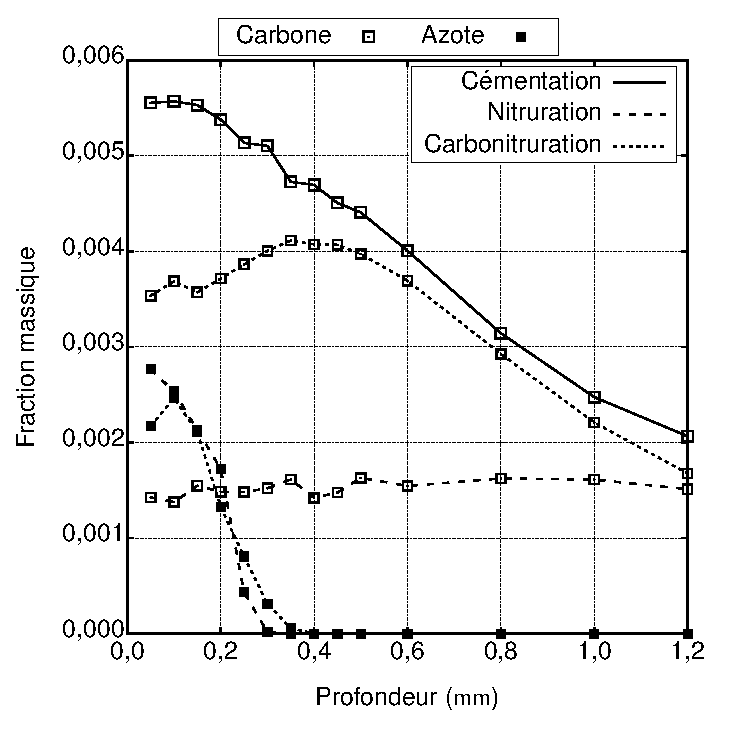
\includegraphics{figures/ch-04-profil_diffusion_aero}}
	}\hfill
	\subfloat[Alliage 23MnCrMo5.]{
		\centering\resizebox{0.48\textwidth}{!}{
			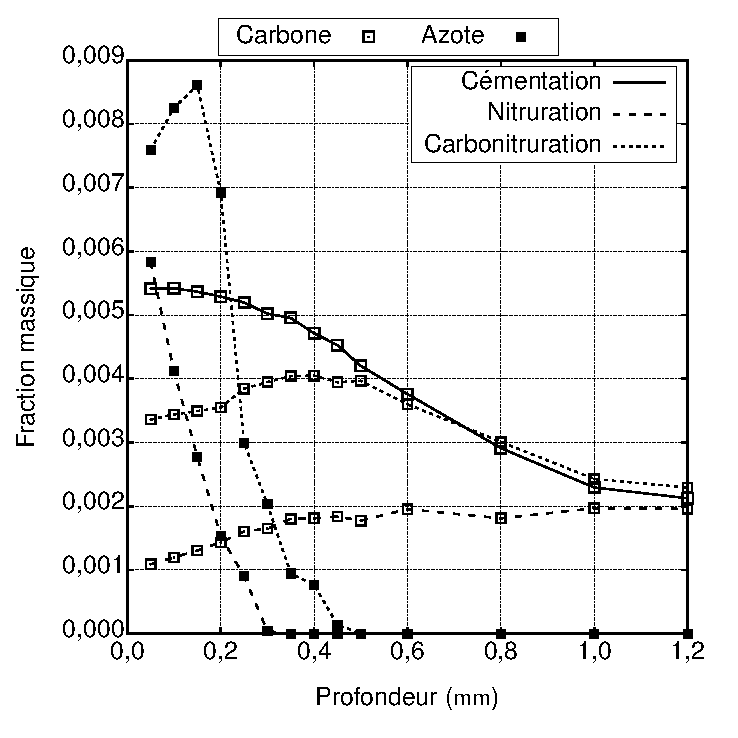
\includegraphics{figures/ch-04-profil_diffusion_auto}}
	}\\
	\subfloat[Simulation alliage 16NiCrMo13.]{
		\centering\resizebox{0.48\textwidth}{!}{
			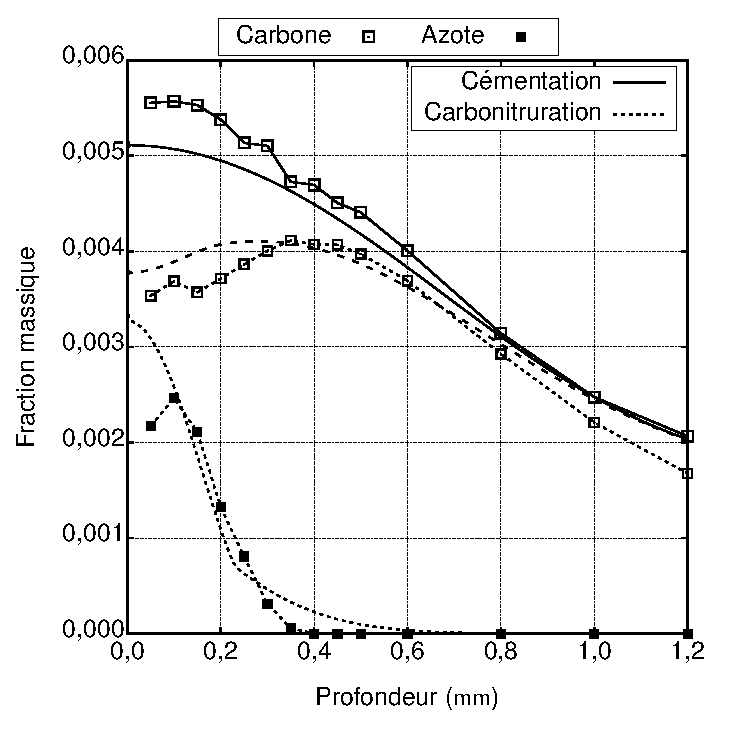
\includegraphics{figures/ch-04-profil_diffusion_sim_aero}}
	}\hfill
	\subfloat[Simulation alliage 23MnCrMo5.]{
		\centering\resizebox{0.48\textwidth}{!}{
			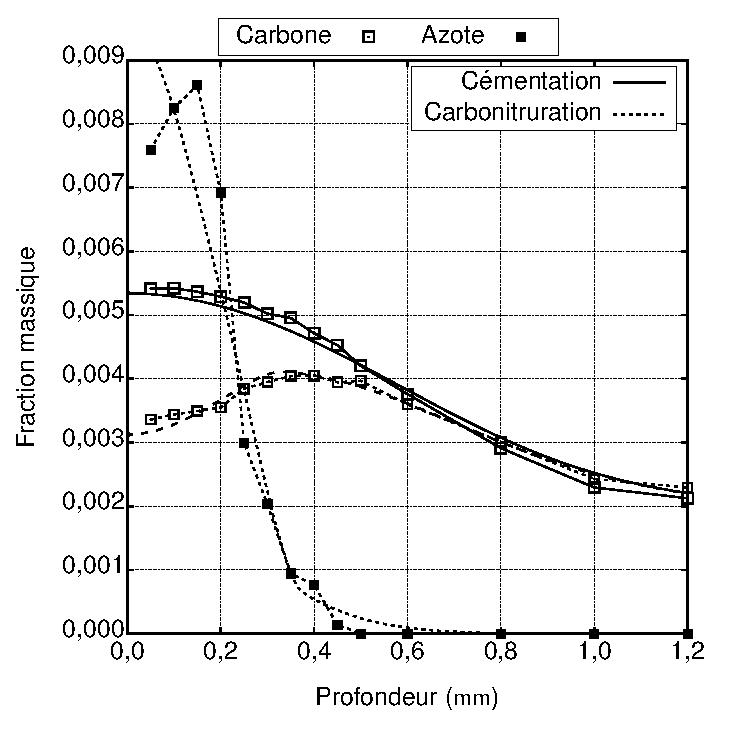
\includegraphics{figures/ch-04-profil_diffusion_sim_auto}}
	}
	
	\caption{\label{fig:diffusion_profiles}Profils de diffusion du carbone et de l'azote après cémentation, nitruration et carbonitruration. Comparaison entre des simulations et mesures expérimentales pour la cémentation et la carbonitruration.}
\end{figure}

\section{Réponses mécaniques}
\label{sec:reponses_mecaniques}

\subsection{Réponse à la trempe}

L'introduction de carbone et d'azote en solution solide permet une diminution de la température de début de transformation martensitique. Par conséquent, la teneur en austénite résiduelle augmente de façon exponentielle \textendash{} comme décrit par l'Équation~\ref{eq:koistinen} attribuée à \citet{Koistinen1959} \textendash{} dans la région traitée. Dans cette étude, on se concentre uniquement sur la réponse mécanique de la martensite, en essayant de minimiser l'austénite résiduelle par une séquence trempe huile -- traitement cryogénique dans l'azote en ébullition. La Figure~\ref{fig:cryogenic_effect_aero} met en évidence le rôle de cette trempe en deux étapes sur la transformation $\gamma_{R}\rightarrow\alpha^{\prime}$ de l'austénite résiduelle $\gamma_{R}$ en martensite $\alpha^{\prime}$ dans une région contenant une fraction massique comprise entre 0,007 et 0,009 en carbone et jusqu'à 0,001 en azote. Figure~\ref{fig:residual-austenite}, on quantifie par analyse d'images une fraction d'environ 35\% d'austénite résiduelle~\footnote{Analyse d'images par conversion de l'image en noir et blanc à travers d'une seuillage des gris manuelle et calcul du rapport des surfaces (en pixels) des zones blanches et de l'image entière.}. Les discussions qui suivent concernent donc des microstructures comme celle de la Figure~\ref{fig:martensite-no-residual}. Dans nos traitements, en général la teneur totale en interstitiels dans les pièces traitées reste en dessous d'une fraction massique d'environ 0,0055, le point-H~\cite{Sherby2008}, et donc les microstructures de départ après trempe huile (\SI{298}{\kelvin}) sont déjà limitées en austénite résiduelle. Ce n'est qu'à partir de cette composition associée au point-H~\cite{Sherby2008} que la fraction en $\gamma_{R}$ devient importante.

\begin{figure}[!h]
  \centering
  \subfloat[\label{fig:residual-austenite}Après trempe huile.]{
    \centering\resizebox{0.48\textwidth}{!}{
    \begin{tikzpicture}
    \node[anchor=south west,inner sep=0] (image1) at (0.0,0.0) {
      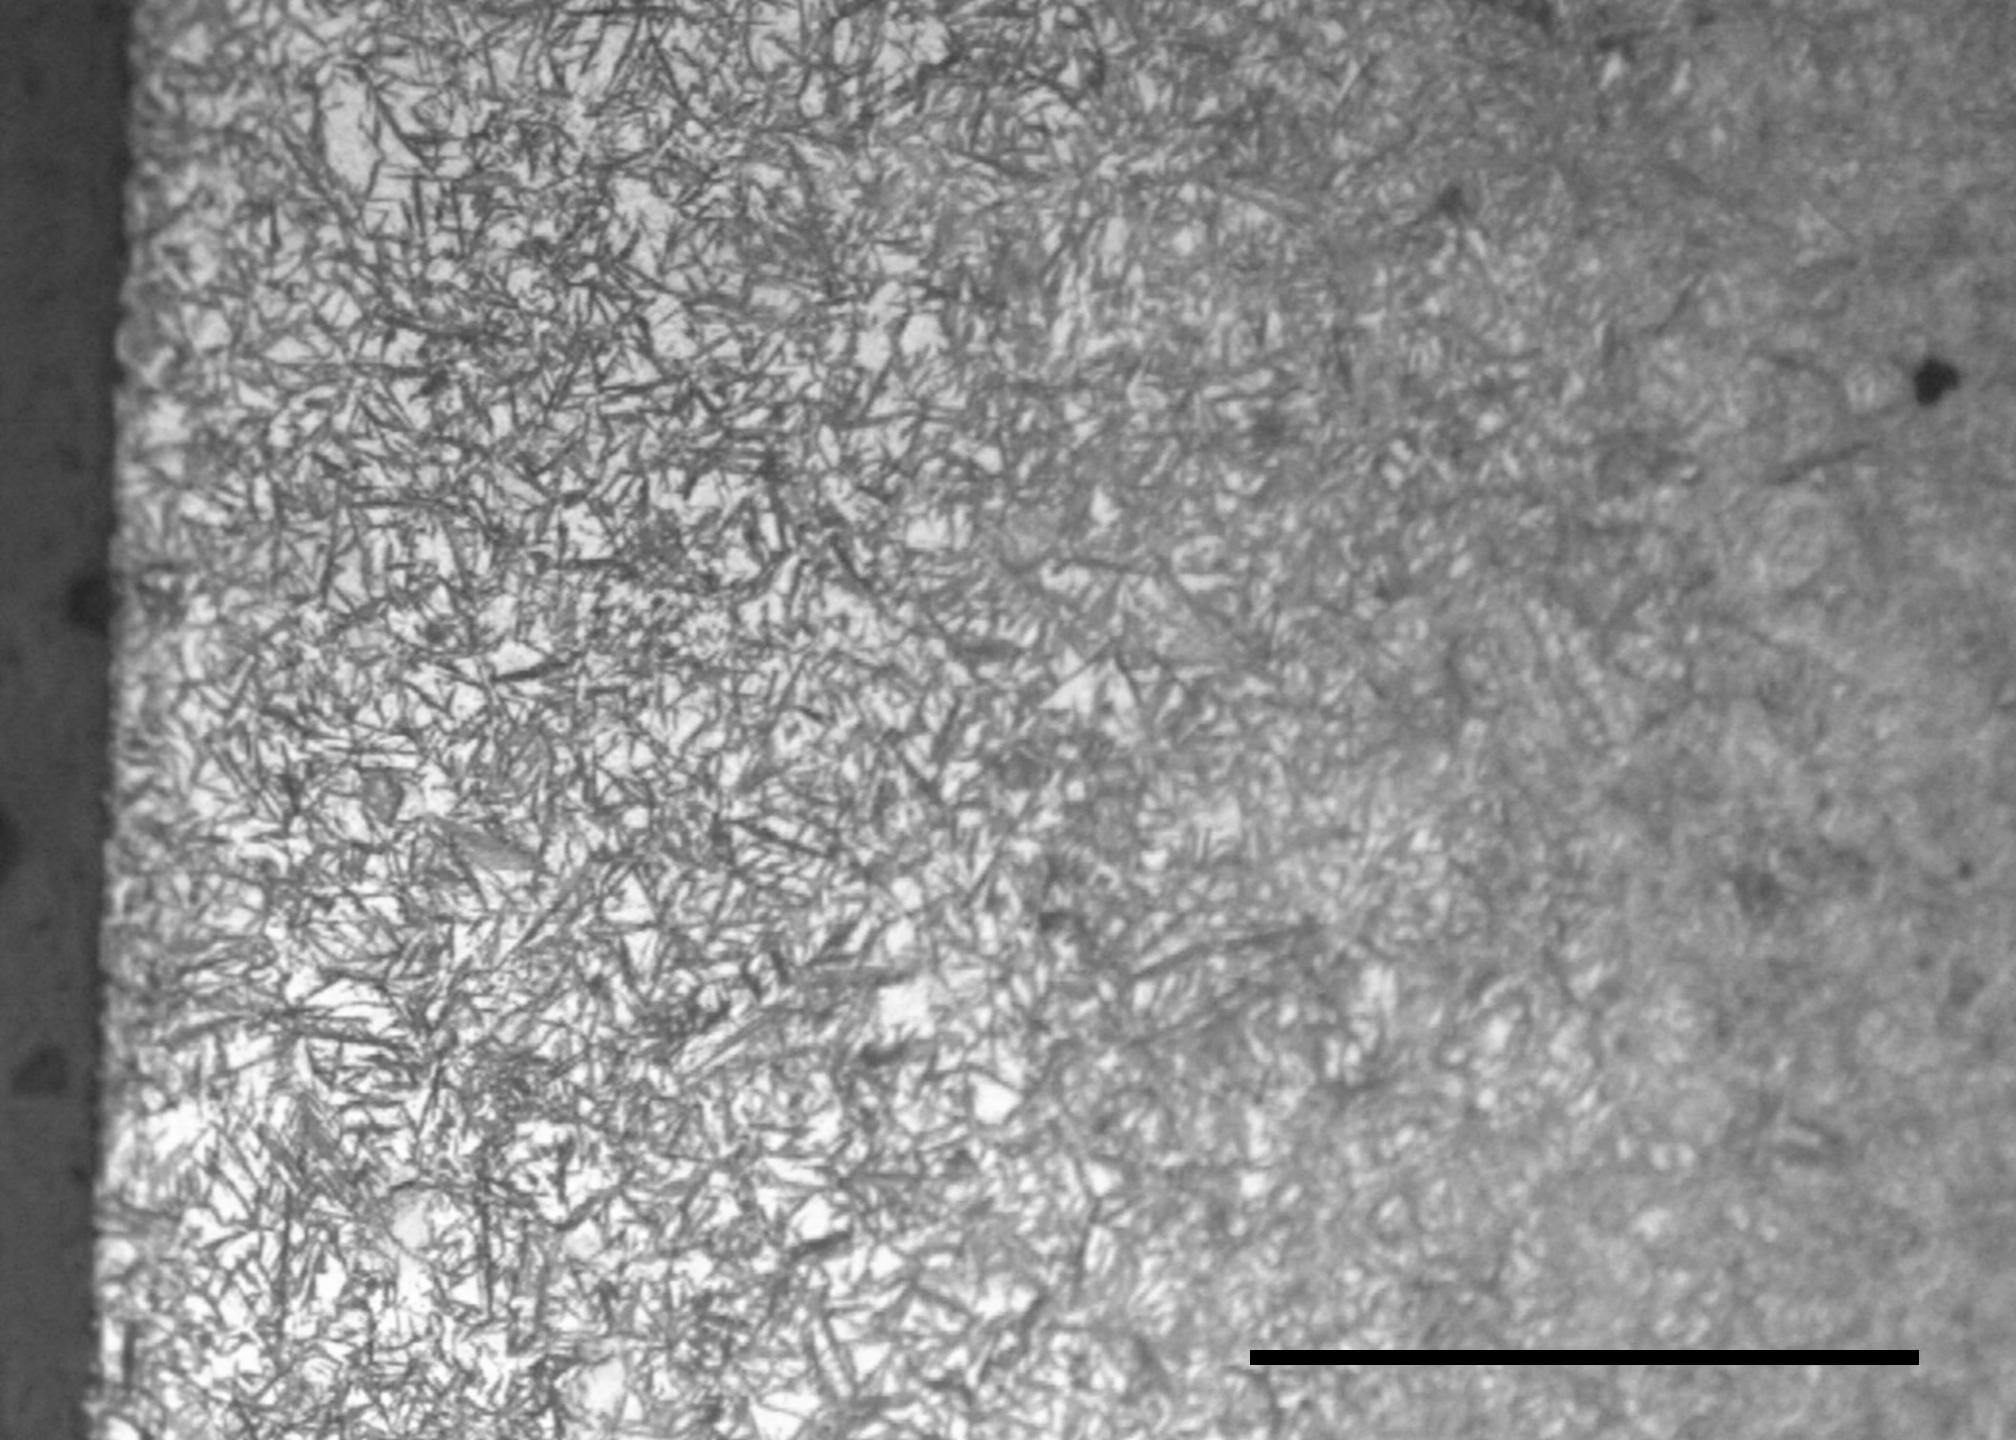
\includegraphics[scale=0.1]{figures/ch-04-aero_carbonitriding_200x_oil}};
    \begin{scope}[x={(image1.south east)},y={(image1.north west)}] 
      \node at (0.8,0.1) {\small\SI{200}{\micro\metre}};
      \node at (0.74, 0.61) {%
        \setlength{\fboxsep}{0pt}
        \setlength{\fboxrule}{2pt}
        \fbox{%
        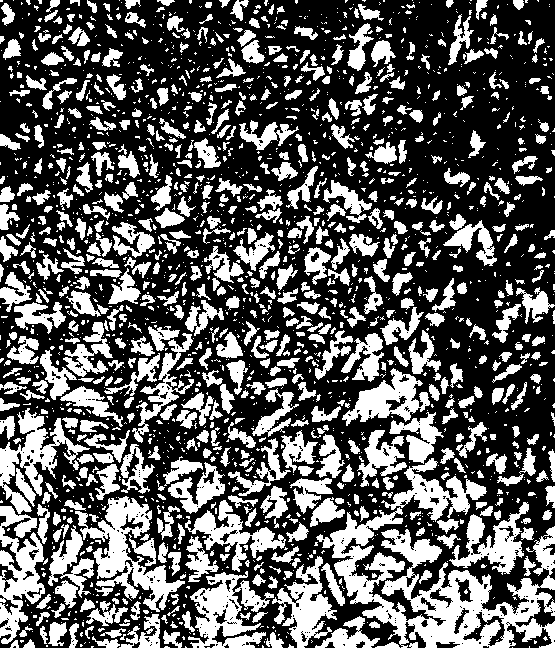
\includegraphics[width=0.2\textwidth]
          {figures/ch-04-aero_carbonitriding_200x_oil_analysis}}
      };
    \end{scope}
    \end{tikzpicture}}
  }\hfill
  \subfloat[\label{fig:martensite-no-residual}Après traitement cryogénique.]{
    \centering\resizebox{0.48\textwidth}{!}{
    \begin{tikzpicture}
    \node[anchor=south west,inner sep=0] (image1) at (0.0,0.0) {
      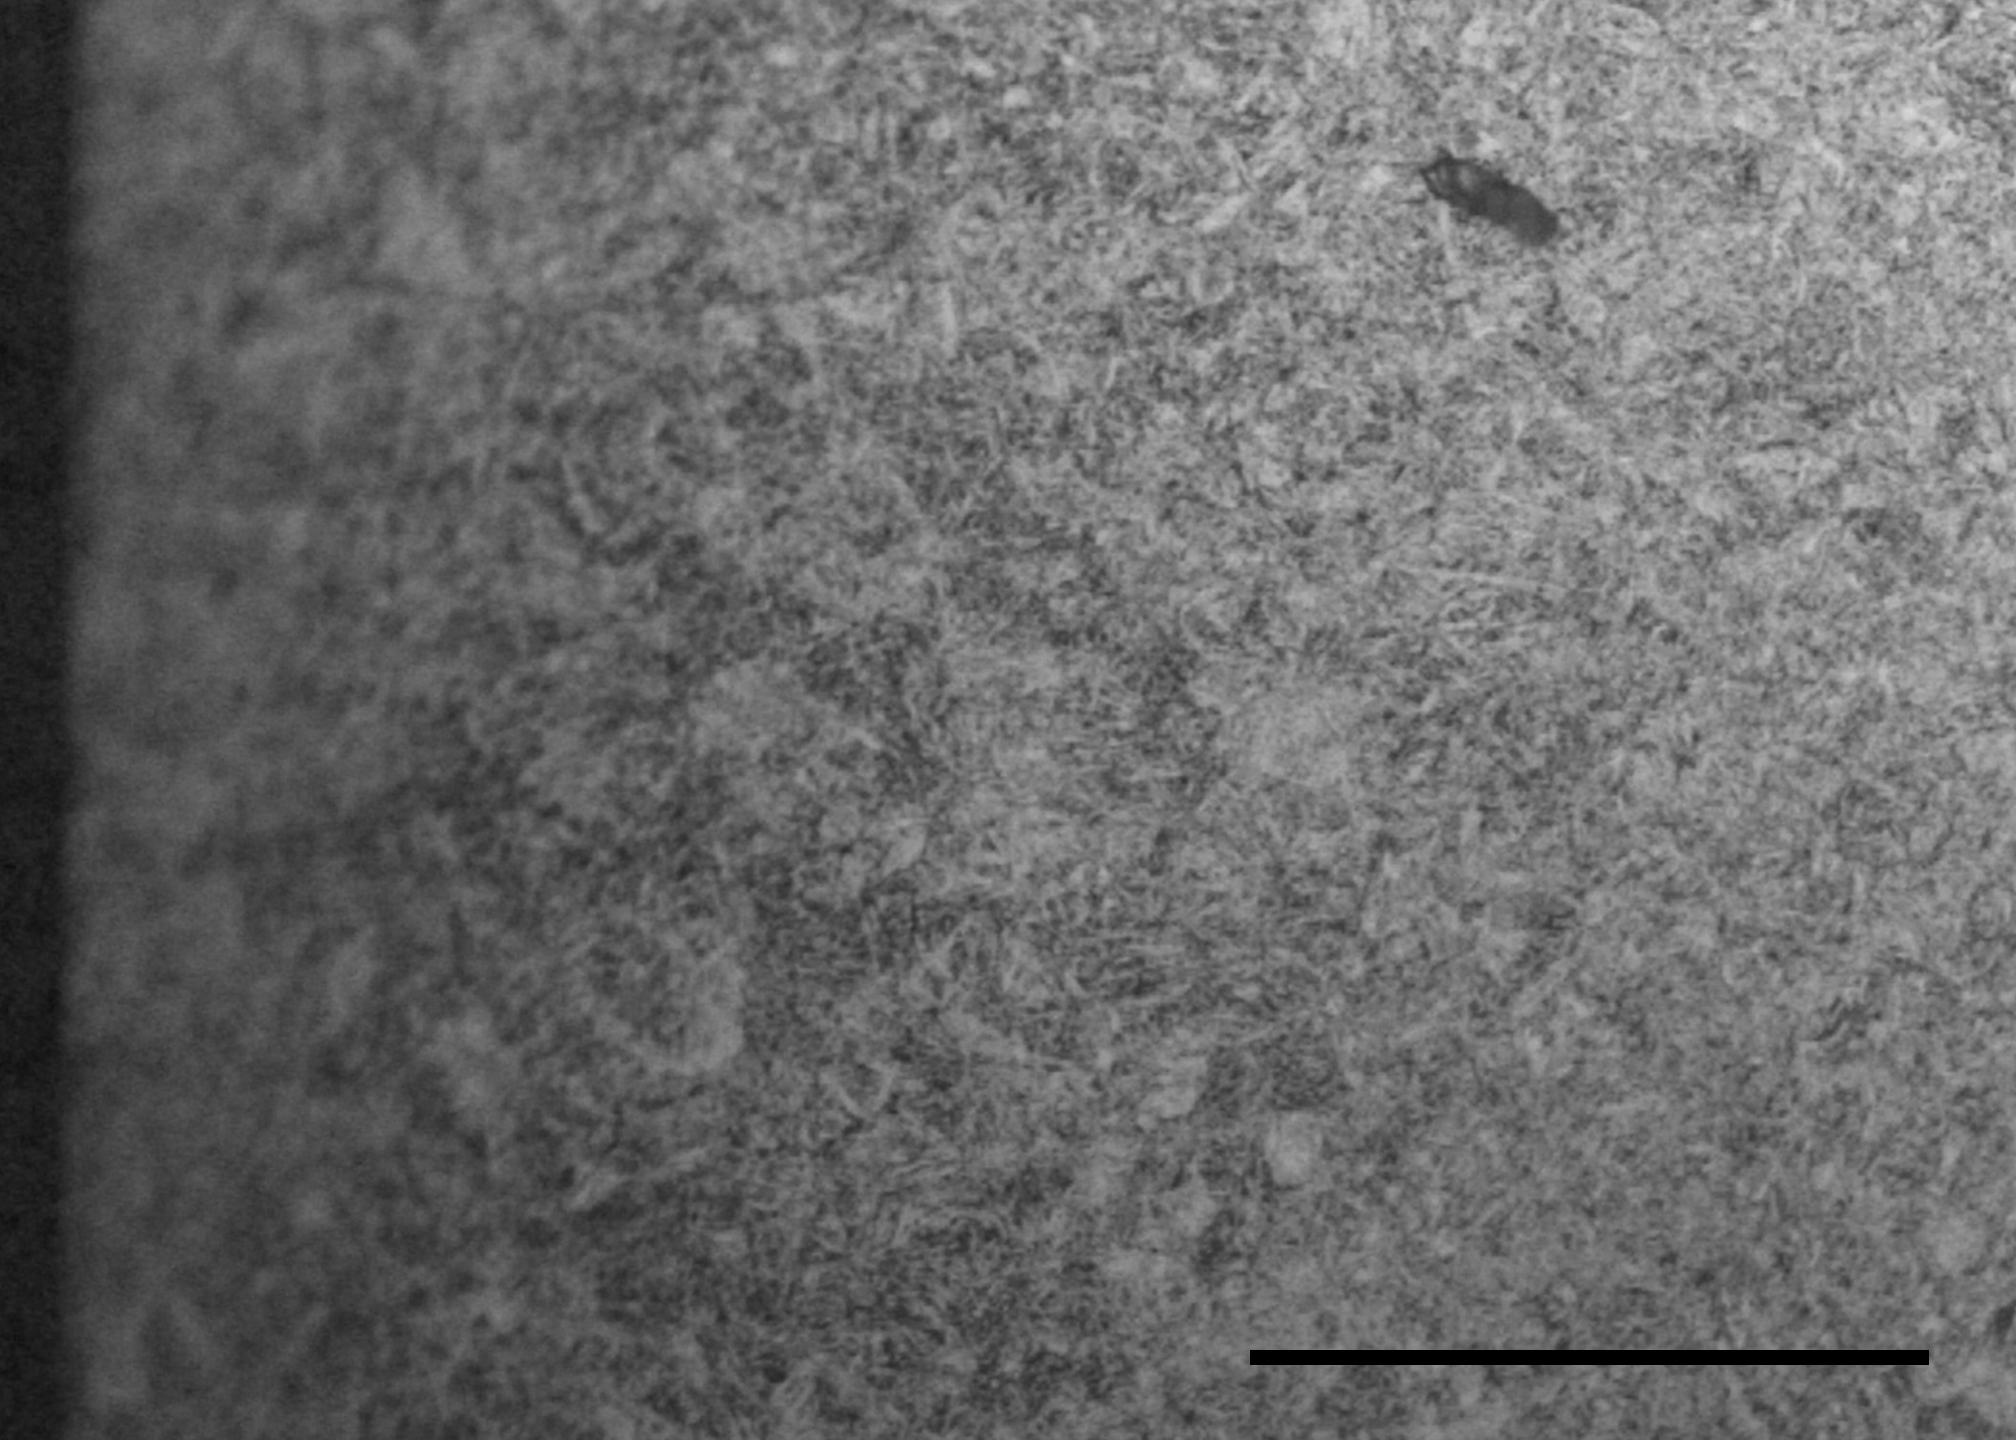
\includegraphics[scale=0.1]{figures/ch-04-aero_carbonitriding_200x_cryo}};
    \begin{scope}[x={(image1.south east)},y={(image1.north west)}] 
    \node at (0.8,0.1) {\small\SI{200}{\micro\metre}};
    \end{scope}
    \end{tikzpicture}}
  }
  
  \caption{\label{fig:cryogenic_effect_aero}Microstructure de l'alliage 16NiCrMo13 enrichi par une fraction massique en carbone donnée en surface après trempe à l'huile à température ambiante et après traitement cryogénique. Microscope optique en lumière visible \textendash{} grandissement de 200$\times$. Le détail à droite de la Figure~\ref{fig:residual-austenite} présente l'image utilisée pour la quantification de $\gamma_{R}$.}
\end{figure}

Les filiations de dureté de la martensite à l'état trempé sont présentées Figure~\ref{fig:hardness_as_quenched} et se trouvent être en bon accord avec des valeurs typiques rapportées dans la littérature~\cite{Grange1977,Krauss1999,Hutchinson20115845,Ferro2014} pour la martensite \ch{Fe-C} et des aciers faiblement alliés. On vérifie Figure~\ref{fig:hardness_as_quenched} le comportement complémentaire du carbone et de l'azote dans l'établissement de la dureté après trempe: la dureté est conservée comme celle de la cémentation en surface des pièces carbonitrurées malgré la décarburation mise en évidence pendant l'introduction de l'azote, ce qui montre la capacité de cet élément à substituer le carbone. En extrême surface (\SI{0,2}{\milli\metre}) de l'alliage 16NiCrMo13, on met en évidence une chute de dureté pour les deux traitements qui est plus prononcée pour la carbonitruration. Cela peut s'expliquer par la formation d'austénite résiduelle~\footnote{À partir de l'Équation~\ref{eq:koistinen}, on montre que pour une teneur en carbone et une température de trempe données, le rapport $r_{\gamma_{R}}$ entre les fractions volumiques d'austénite résiduelle prédites pour les alliages 16NiCrMo13 et 23MnCrMo5 est donnée par $r_{\gamma_{R}}=\exp\big[-1,1\times 10^{-2}(M_{s,\mathrm{16NiCrMo13}}-M_{s,\mathrm{23MnCrMo5}})\big]$. Si l'on considère, par exemple, la formule d'\citet{Andrews1965} pour le calcul de la température d'initiation de la réaction martensitique $M_s$ pour chaque alliage en fixant une teneur en carbone, on montre que ce rapport est de l'ordre de 1,4 -- l'alliage 16NiCrMo13 retient 40\% d'austénite résiduelle de plus que la nuance 23MnCrMo5.}. 
On a présenté Section~\ref{sec:martensite_cn} le modèle de durcissement utilisé pour expliquer la réponse à la trempe dans notre cas: la dureté de la martensite doit augmenter de façon linéaire avec la racine carrée de la fraction molaire $x_{i}$ en interstitiels dissous. On applique le raisonnement de \citet{Hutchinson20115845} qui suppose que les atomes interstitiels en solution solide se comportent comme des agglomérats capables de bloquer le mouvement des dislocations, ces agglomérats contribuent à augmenter la résistance mécanique selon une dépendance en racine carrée de leur teneur~\cite{Haasen19962009}. Comme évoqué par les auteurs~\cite{Hutchinson20115845}, ces atomes ne sont pas nécessairement dans les sites octaédriques de la martensite, mais dans les défauts cristallins sous forme d'atmosphères de Cottrell, stoppant le glissement des dislocations. Par ailleurs, \citet{Morito20031475} montrent une dépendance linéaire entre la teneur en carbone et la densité de dislocations $\rho$ qui augmente aussi en racine carrée la résistance mécanique des alliages~\cite{Cohen1968,Norstrom1976,Krauss1999,Hutchinson20115845}. On a donc ces deux phénomènes complémentaires produisant la réponse en dureté de la martensite trempée selon un même type de dépendance: la racine carrée de la teneur en interstitiels dissous. 

\begin{figure}[h]
  \subfloat[Alliage 16NiCrMo13.]{
    \centering\resizebox{0.48\textwidth}{!}{
      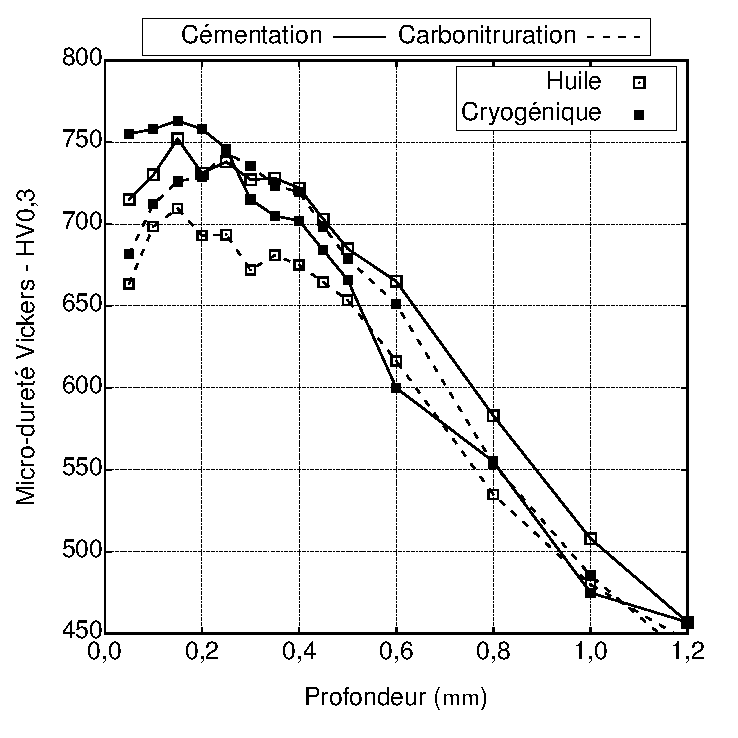
\includegraphics{figures/ch-04-hardness_as_quenched_aero}}
  }\hfill
  \subfloat[Alliage 23MnCrMo5.]{
    \centering\resizebox{0.48\textwidth}{!}{
      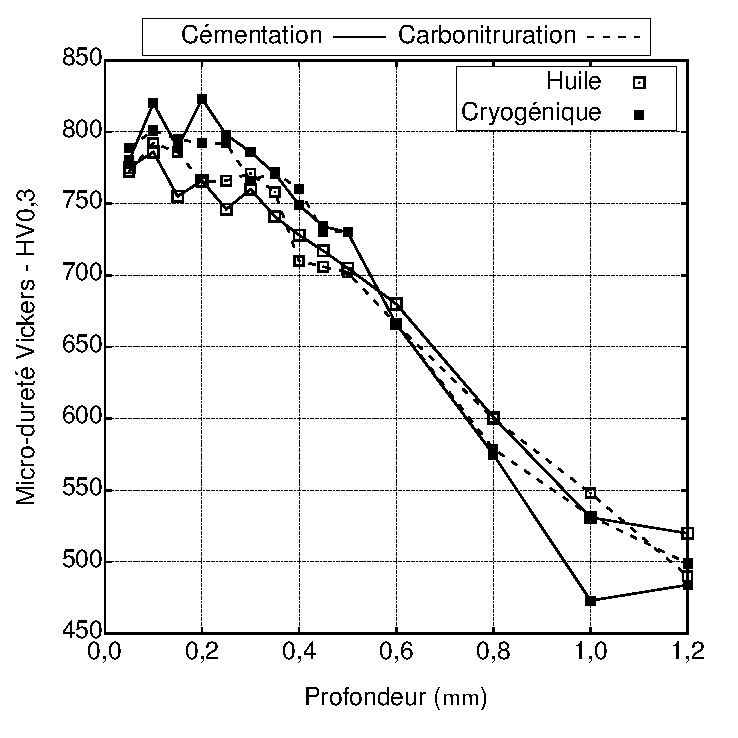
\includegraphics{figures/ch-04-hardness_as_quenched_auto}}
  }

  \caption{\label{fig:hardness_as_quenched}Dureté après cémentation et carbonitruration suivies d'une trempe à l'huile et traitement cryogénique en fonction de la distance à la surface des pièces traitées.}
\end{figure}

On fait l'hypothèse que ce comportement peut aussi être attribué à l'azote en solution solide en dessous du point-H~\cite{Sherby2008}, i.e. dans la région du domaine martensitique cubique, à partir duquel la croissance rapide de la teneur en austénite résiduelle s'écarte de la réponse linéaire de la limite élastique avec la racine carrée en interstitiels. On généralise la relation proposée par \citet{Cohen1968,Norstrom1976} en ajoutant la dépendance avec la fraction en azote. Il est clair que cette approche n'est possible que si l'on utilise des fractions molaires $x_{i}$, avec $i = (\ch{C},\ch{N})$: c'est le nombre d'atomes en solution qui constitue la variable régissant la limite élastique. Cette hypothèse faite, il nous est nécessaire de connaître l'azote dissous en solution solide. C'est là que réside l'importance de l'utilisation de Thermo-Calc~\cite{Andersson2002,Borgenstam2000} et de l'obtention de profils de diffusion simulés en bon accord avec les mesures expérimentales: une allure \og{}correcte\fg{} du profil de diffusion de l'azote simulée traduit une prédiction \og{}correcte\fg{} des nitrures formés pendant l'enrichissement en azote et donc une bonne valeur de l'azote en solution solide qui pourra être utilisée dans le modèle de durcissement. 

Il faut remarquer que la précision des profils de diffusion n'a pas de lien direct avec l'adéquation des conditions aux limites. Comme on l'a montré Section~\ref{sec:comparaison_procedes}, l'activité de l'atmosphère ne correspond pas à la teneur en surface obtenue dans l'alliage 16NiCrMo13, bien que le profil de diffusion simulé pour $a_{N}=10$ semble décrire correctement l'allure des mesures réalisées par EPMA sur la Figure~\ref{fig:diffusion_profiles}: on suppose donc que la prédiction du comportement de l'azote en diffusion-précipitation est correcte, la condition aux limites étant différente de celle fournie par la thermodynamique de l'atmosphère. En fonction de ces résultats, Thermo-Calc~\cite{Andersson2002,Borgenstam2000} a été utilisé pour simuler la teneur en interstitiels en solution solide pour chaque point rapporté Figure~\ref{fig:diffusion_profiles}. D'autres contributions, i.e. durcissement par solution solide promu par les éléments d'alliage, morphologie de la martensite, etc. sont ici considérés comme négligeables. La Figure~\ref{fig:hardness_norstrom} présente la dépendance de la dureté (ici supposée proportionnelle à la limite élastique) avec $x_{i}^{0.5}$, la racine carrée de la fraction molaire totale d'éléments interstitiels en solution solide. 

Les éléments carbone et azote sont considérés comme possédant une capacité de blocage des dislocations similaires du fait de leur taille dans l'austénite: l'azote possède un rayon environ 5-7\% supérieur à celui du carbone~\cite{Yahia1995}. Une étude exhaustive pourrait permettre l'introduction d'un coefficient pour chaque élément, ce qui n'a pas été fait ici. On observe deux régions principales Figure~\ref{fig:hardness_norstrom}, la première à gauche de $\mathrm{x_{i}^{0,5}=0,16}$, où le modèle de \citet{Norstrom1976} est valable et la dureté augmente de façon linéaire avec le paramètre $x_{i}^{0,5}$ puis, la seconde au-delà de cette limite où l'on trouve un plateau de durcissement et même une chute en dureté pour des fractions plus élevées en interstitiels. Un deuxième axe est ajouté en haut de la Figure~\ref{fig:hardness_norstrom} pour donner la fraction massique estimée correspondant à chaque $x_{i}^{0,5}$, la conversion précise n'étant pas possible en raison des différentes masses des éléments en solution. Le point-H~\cite{Sherby2008} est identifié sur la figure, indiquant la limite pratique d'amélioration de la limite élastique des surfaces des aciers faiblement alliés sans que des traitements cryogéniques soient réalisés. À partir de $x_{i}^{0,5}=0,18$ une chute importante en dureté est mise en évidence pour l'alliage 16NiCrMo13 en raison de la présence de l'austénite résiduelle. Sa décomposition rend possible l'augmentation de la dureté au niveau du plateau formé à \SI{850}{\HV}. 

\begin{figure}[h]
  \centering
  \resizebox{0.98\textwidth}{!}{
    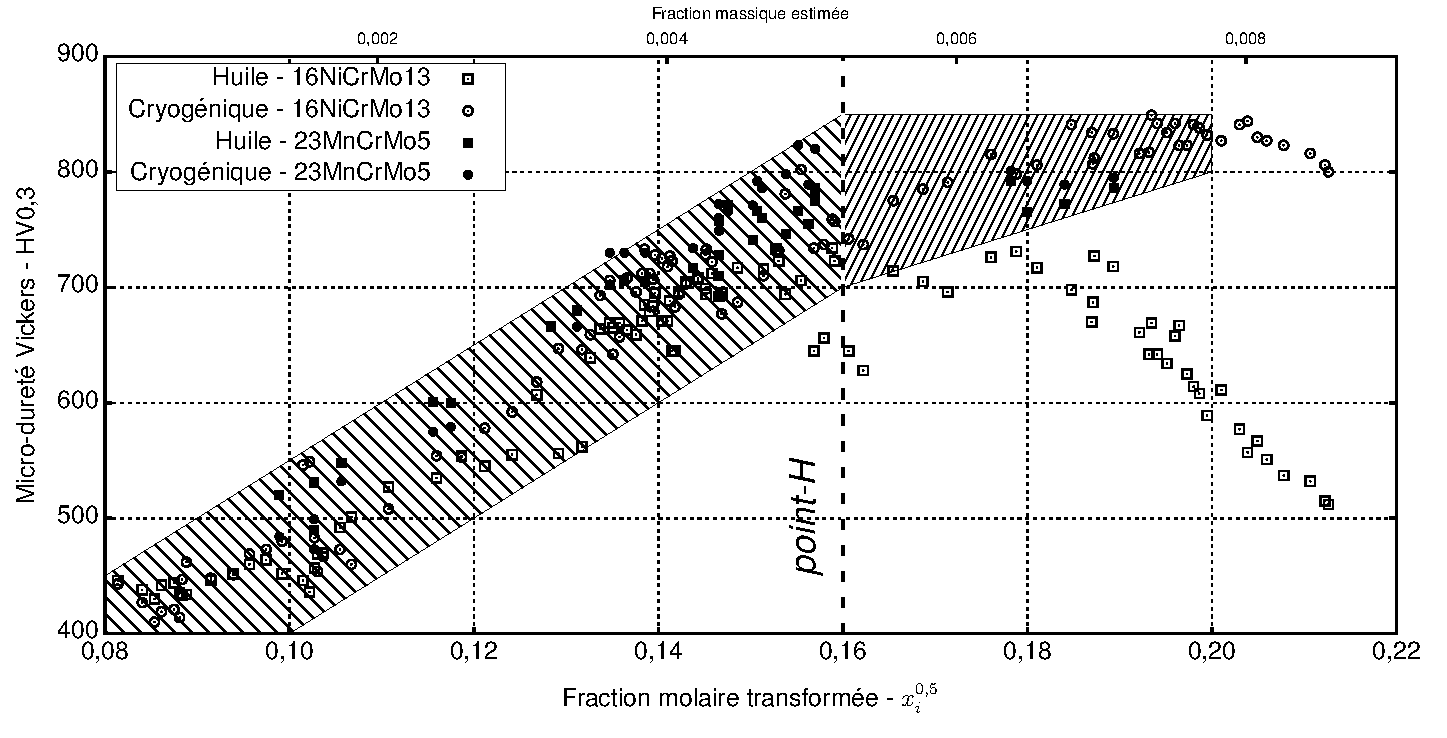
\includegraphics{figures/ch-04-hardness_norstrom}}
  
  \caption{\label{fig:hardness_norstrom}Dureté après trempe à l'huile et traitement cryogénique en fonction de la racine carrée de la somme des fractions molaires en carbone et en azote en solution solide juste avant trempe.  Les données d'entrée pour l'azote sont issues de simulations à l'aide de Thermo-Calc~\cite{Andersson2002,Borgenstam2000}. Les points sont issus de toutes les gammes de traitement réalisées, sans faire la distinction entre les enrichissements par un élément interstitiel spécifique.}
\end{figure}

\subsection{Réponse au revenu}

Bien que la dureté à l'état trempé puisse être expliquée par la composition locale, le revenu induit une série de processus plus complexes conduisant normalement à une chute de dureté sur toute la profondeur enrichie, comme cela est présenté Figure~\ref{fig:hardness_temper} pour la cémentation et la carbonitruration \textemdash{} l'état de référence choisi correspond à la dureté obtenue après traitement cryogénique. Une chute en dureté moins importante est observée pour la carbonitruration sur la zone enrichie en azote \textendash{} voir Figure~\ref{fig:diffusion_profiles} \textendash{} si on la compare à la cémentation, effet qui est particulièrement prononcé pour les deux conditions de revenu de l'alliage 23MnCrMo5. Dans ce cas, même si la dureté de départ \textendash{} après traitement cryogénique \textendash{} est de l'ordre de \SI{800}{\HV} pour les deux traitements thermochimiques, les profils enrichis en azote préservent un gain en dureté sur une profondeur de \SI{0,3}{\milli\metre} d'environ \SI{70}{\HV} par rapport à la dureté à c{\oe}ur.

\begin{figure}[h]
  \centering
  \subfloat[Alliage 16NiCrMo13.]{
    \centering\resizebox{0.48\textwidth}{!}{
    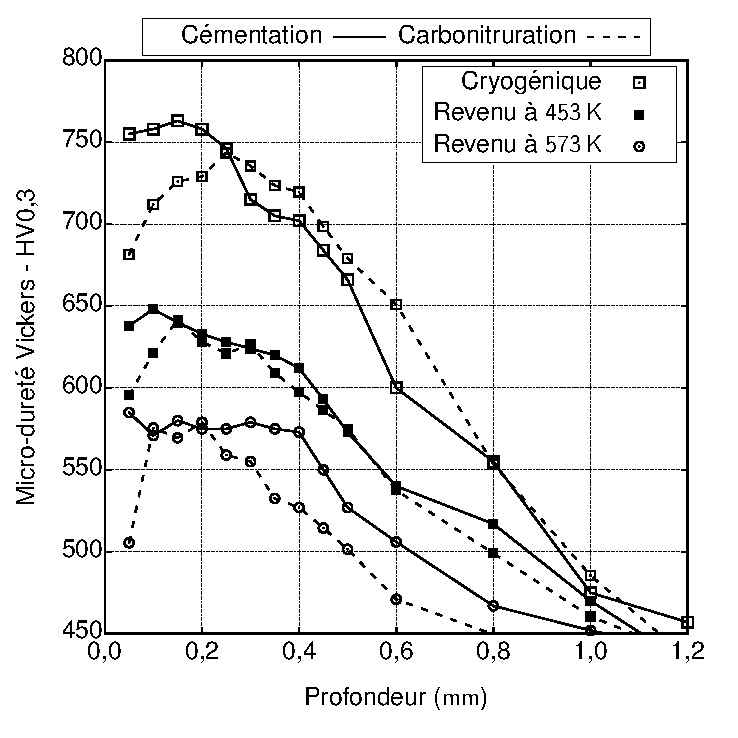
\includegraphics{figures/ch-04-hardness_temper_aero}}
  }\hfill
  \subfloat[Alliage 23MnCrMo5.]{
    \centering\resizebox{0.48\textwidth}{!}{
    \includegraphics{figures/ch-04-hardness_temper_auto}}
  }
  
  \caption{\label{fig:hardness_temper}Dureté après cémentation et carbonitruration suivies soit d'un traitement cryogénique soit d'un revenu en fonction de la distance à la surface des pièces traitées.}
\end{figure}

L'alliage 23MnCrMo5 a été enrichi à environ 0,8~\%~N en poids en surface. Si l'on considère la formation de nitrures de type \ch{MN}, cela devrait réduire le chrome en solution à moins de 0,3~\% en poids et une martensite moins stable au revenu est alors attendue~\cite{Grange1977}. Comme cela a été montré par \citet{Catteau2016}, même pour des teneurs plus faibles en azote, cet alliage devrait précipiter aussi des nitrures mixtes \ch{MnSiN2}, qui devrait accroître d'autant l'appauvrissement de la matrice en éléments carburigènes capables de retarder la cinétique de revenu par la précipitation de carbures. On observe Figure~\ref{fig:microstructure-auto-quenched} une forte densité de particules submicrométriques \textendash{} elles seront caractérisées par microscopie électronique en transmission \textendash{} sur une profondeur de \SI{300}{\micro\metre}. Par conséquent, le revenu de cet alliage doit être gouverné par une matrice moins riche en éléments d'alliage et doit présenter un comportement proche de celui du fer pur, pour lequel une précipitation de \ch{Fe16N2} cohérent à basse température est attendue. Ce type de précipité devient incohérent dans les premiers instants du revenu et est finalement converti à l'équilibre en \ch{Fe4N}~\cite{Kaplow1983,vanGent1985,Mittemeijer1988,Cheng199013,Cheng19902857,Fall1996,vanGenderen1997}. Cette séquence ne peut pas expliquer les réponses mécaniques obtenues: on peut alors penser soit à une \og{} dureté composite \fg{} entre la matrice et les précipités présents à forte concentration, soit à une transformation retardée par présence d'éléments d'alliage, la phase \ch{Fe16N2} cohérente pouvant alors apporter un durcissement comme dans le cas du système \ch{Fe-N}~\cite{Mittemeijer2010}. 

\begin{figure}[h]
  \resizebox{0.98\textwidth}{!}{
    \iftoggle{paper}
    {\includegraphics{figures/ch-04-micrograph_auto_quenched-pdf}} % print
    {\includegraphics{figures/ch-04-micrograph_auto_quenched-png}} % digital
  }
  
  \caption{\label{fig:microstructure-auto-quenched}Gradient de précipités formés pendant l'enrichissement de l'alliage 23MnCrMo5 carbonitruré. On observe une forte densité de points sombres sur les micrographies à \SI{0}{\micro\metre} et à \SI{100}{\micro\metre} suivi d'une décroissance jusqu'à une microstructure majoritairement martensitique à \SI{100}{\micro\metre}.  Microscope optique en lumière visible \textendash{} grandissement de 1250$\times$.}
\end{figure}

\subsection{Réponse à la nitruration}

Les réponses mécaniques à la nitruration austénitique sont traitées à part dans cette section relativement au comportement mis en évidence: alors que les enrichissements uniquement en carbone ou combinés carbone-azote ont conduit a une chute en dureté sur toute la profondeur enrichie lors du revenu, les échantillons nitrurés montrent un maintien de la dureté proche de celle de l'alliage trempé si la température de revenu est supérieure à \SI{573}{\kelvin}. Le revenu équivalent determiné à partir du paramètre d'Hollomon \textendash{} constante d'Hollomon-Jaffe supposée égale à 20~\cite{Wan2005,Steel2006} \textendash{} est plus important avec le traitement réalisé à \SI{573}{\kelvin} (\SI{18}{\hour}) par rapport à celui fait à \SI{453}{\kelvin} (\SI{70}{\hour}). De cette façon, un revenu plus prononcé des matériaux était attendu à \SI{573}{\kelvin}, ce qui n'est pas le cas sur toute la profondeur enrichie en azote \textemdash{} Figure~\ref{fig:hardness_nitriding}. 

\begin{figure}[!b]
  \centering
  \subfloat[Alliage 16NiCrMo13.]{
    \centering\resizebox{0.48\textwidth}{!}{
      \includegraphics{figures/ch-04-hardness_nitriding_aero}}
  }\hfill
  \subfloat[Alliage 23MnCrMo5.]{
    \centering\resizebox{0.48\textwidth}{!}{
      \includegraphics{figures/ch-04-hardness_nitriding_auto}}
  }
  
  \caption{\label{fig:hardness_nitriding}Dureté après nitruration suivie soit par un traitement cryogénique, soit par un traitement cryogénique et un revenu en fonction de la distance à la surface des pièces.}
\end{figure}

La confirmation du phénomène se fait en réalisant un revenu à \SI{673}{\kelvin} pendant \SI{18}{\hour}. La dureté ainsi obtenue est conservée proche de celle après trempe en surface, ce qui peut être lié à une précipitation secondaire. On observe un déplacement du maximum de dureté vers le c{\oe}ur des pièces, ce qui est lié à la coalescence/transition cohérent-incohérent en extrême surface des précipités formés et à la mobilité atomique \textendash{} diffusion de l'azote vers le c{\oe}ur \textendash{}. Finalement, la dureté dans la zone non-nitrurée chute de manière plus importante qu'à plus faible température \textemdash{} en augmentant la température de revenu on diminue progressivement la dureté de la zone au-delà de \SI{0,3}{\milli\metre}. Cette séquence est valable pour les deux alliages étudiés et est plus prononcée pour la nuance 16NiCrMo13, ce qui est possiblement lié à la plus faible teneur en carbone \textendash{} ce comportement n'a pas été mis en évidence lors de la carbonitruration des alliages. Ce comportement peut permettre de comprendre l'amélioration de la résistance au revenu produite par la carbonitruration.

\section{Identification des précipités}
\label{sec:precipitation}

Suite aux résultats de la Section~\ref{sec:reponses_mecaniques}, une étude en  microscopie électronique en transmission ont été réalisées. L'étude vise tout d'abord à identifier les précipités formés à haute température lors des traitements thermochimiques, ce qui s'accompagne d'une consommation des éléments d'alliage de la matrice. Cela comprend des cartographies d'émission de rayons-x obtenues à partir des spectres EDX en mode STEM, permettant d'identifier la redistribution des éléments pour former des précipités de taille sub-micrométrique. Ensuite, l'imagerie en mode TEM et la diffraction d'électrons permettent l'identification des précipités nanométriques cohérents formés lors du revenu, ce qui peut expliquer les filiations de dureté observées pour les traitements avec enrichissement en azote.

\subsection{Alliage 23MnCrMo5 carbonitruré}

Suite à l'observation de précipités dans une échelle sub-micrométrique Figure~\ref{fig:microstructure-auto-quenched}, des cartographies d'émission de rayons-x ont été obtenues dans la région riche en azote de la nuance 23MnCrMo5 carbonitrurée, plus spécifiquement à \SI{100}{\micro\metre} de la surface pour éviter de possibles effets de dénitruration/oxydation en surface. Ces résultats sont présentés Figure~\ref{fig:chemical-maps-auto}, où on met en évidence la formation de zones riches simultanément en chrome et en azote, et d'autres contenant également les éléments manganèse et silicium. Les nitrures sont identifiés comme ayant une st{\oe}chiométrie du type \ch{MN}. Ils sont composés de manière prépondérante de chrome et d'azote et de \ch{MnSiN2} (groupe spatial $Pna2_{1}$~\cite{Weitzer1987178}), comme cela a déjà été mis en évidence par \citet{Catteau2016} pour des teneurs en azote d'environ 0,25~\% en poids. Aucune preuve de la présence de nitrures de type \ch{Si3N4} comme cela est prédit par Thermo-Calc~\cite{Andersson2002,Borgenstam2000} avec la base de données TCFE7, ou de \ch{VN} comme rapporté par \citet{Catteau2016} n'a été apportée. On observe Figure~\ref{fig:chemical-maps-auto} la présence de deux tailles caractéristiques de précipités, l'une associée aux nitrures \ch{MN} de dimensions de l'ordre de \SI{100 x 50}{\nano\metre} et l'autre associée aux précipités \ch{MnSiN2} de \SIrange{200}{1000}{\nano\metre} de dimensions caractéristiques.

\begin{figure}[!ht]
  \centering\resizebox{0.98\textwidth}{!}{
    \iftoggle{paper}
    {\includegraphics{figures/ch-04-TEM/x-tem_auto_cartography/figure.pdf}} % print
    {\includegraphics{figures/ch-04-TEM/x-tem_auto_cartography/figure.png}} % digital
  }
  
  \caption{\label{fig:chemical-maps-auto}Cartographie d'émission des rayons x caractéristiques des éléments constituant les nitrures de type \ch{MN} (avec \ch{M} majoritairement \ch{Cr}) et de type \ch{MnSiN2} formés pendant la carbonitruration de l'alliage 23MnCrMo5. Fraction massique en azote de 0,80\% en poids dans la région analysée.}
\end{figure}

\subsection{Alliage 16NiCrMo13 nitruré}

\begin{figure}[!b]
  \centering\resizebox{0.98\textwidth}{!}{
    \iftoggle{paper}
    {\includegraphics{figures/ch-04-TEM/x-tem_aero_cartography/figure.pdf}} % print
    {\includegraphics{figures/ch-04-TEM/x-tem_aero_cartography/figure.png}} % digital
  }
  
  \caption{\label{fig:chemical-maps-aero}Cartographie d'émission des rayons x caractéristiques des éléments constituant les nitrures de type \ch{MN} (avec \ch{M} majoritairement \ch{Cr}) formés pendant la nitruration de l'alliage 16NiCrMo13. Fraction massique en azote de 0,25\% en poids.}
\end{figure}

Comme pour la nuance 23MnCrMo5, la redistribution des éléments d'alliage lors de l'enrichissement en azote a été observée par analyse d'émission des raies de rayons x pour l'alliage 16NiCrMo13 nitruré. Dans le cas de cet alliage, seuls des nitrures de type \ch{MN} ont été observés (Figure~\ref{fig:chemical-maps-aero}), en accord avec la prédiction faite par Thermo-Calc~\cite{Andersson2002,Borgenstam2000} à l'aide de la base de données TCFE7, pour la composition de la lame observée.  Ces précipités, de morphologie globulaire ou sous forme de bâtonnet, couvrent une surface entre 1,8\% et 2,5\% de la section transversale des lames. Dès que les régions où les cartographies ont été réalisées atteignent une épaisseur moyenne de \SI{80}{\nano\metre} et si l'on suppose que tous les précipités \ch{MN} dans le volume sont détectés, alors une estimation de leur fraction volumique peut être faite par analyse d'images. On obtient qu'entre 0,8\% et 1,0\% de précipités sont formés. Thermo-Calc~\cite{Andersson2002,Borgenstam2000} prédit une fraction volumique autour de 1,0\% pour la composition locale, ce qui est assez proche de la valeur estimée par analyse des cartographies de rayons x. Cela implique une précipitation à l'équilibre dans la région étudiée et cela sert à valider l'approche du modèle de durcissement établi pour expliquer la dureté après trempe: les précipités attendus sont déjà formés et donc la prédiction de l'azote dissous dans la martensite est raisonnable.

%\pagebreak

La structure martensitique après trempe et traitement cryogénique de la nuance 16NiCrMo13 après nitruration en phase austénitique a été identifiée comme étant composée de lattes de largeurs typiques allant de \SIrange{200}{500}{\nano\metre} dans une région contenant 0,13\%~C et 0,25\%~N en poids. Ces structures sont présentées Figure~\ref{fig:tem-aero-micro-laths} où le contraste permet de visualiser quelques nitrures \ch{MN} identifiés Figure~\ref{fig:chemical-maps-aero}. L'alliage présente encore (Figure~\ref{fig:tem-aero-micro-shear}-b) des zones de cisaillement d'environ \SI{100 x 10}{\nano\metre} orientées dans deux directions possibles de la martensite, lesquelles sont probablement formées pendant la trempe. Ces zones correspondent à la structure ordonnée \ch{Fe16N2} et un détail de leur morphologie est présenté en haute résolution Figure~\ref{fig:tem-aero-micro-shear}-d, d'où le cliché de diffraction de la Figure~\ref{fig:tem-aero-micro-shear}-c a été obtenu. Bien que ces régions puissent se comporter comme barrières au glissement des dislocations, elles ne permettent pas d'expliquer le comportement en durcissement observé lors du revenu. Cela vient du fait que ces zones de cisaillement ont aussi été observées avant le revenu. %, juste après enrichissement.

\begin{figure}[h]
  \centering\resizebox{0.6\textwidth}{!}{
    \iftoggle{paper}
    {\includegraphics{figures/ch-04-TEM/x-tem_aero_mesoscale-laths/figure.pdf}} % print
    {\includegraphics{figures/ch-04-TEM/x-tem_aero_mesoscale-laths/figure.png}} % digital
  }

  \caption{\label{fig:tem-aero-micro-laths}Micrographies de l'alliage 16NiCrMo13 nitruré, trempé et soumis au traitement cryogénique: (a) fond clair en mode STEM, mettant en évidence la structure martensitique en lattes ($\times$120k), (b) nitrure \ch{MN} formé à la température d'enrichissement (grandissement de $\times$100k).}
\end{figure}

Les structures de la Figure~\ref{fig:tem-aero-micro-shear} sont prises comme état de référence pour l'étude des échantillons soumis au revenu au-dessus de \SI{573}{\kelvin}: on cherche des caractéristiques pour ces dernières qui ne sont pas présentes avant le revenu. On vérifie Figure~\ref{fig:tem-aero-nano} dans la matrice martensitique cubique centrée de l'alliage 16NiCrMo13 nitruré et soumis au revenu à \SI{573}{\kelvin} la présence d'une multitude de précipités nanométriques \textendash{} moins de \SI{5}{\nano\metre} \textendash{} qui n'ont pas été détectés dans la lame correspondant à la Figure~\ref{fig:tem-aero-micro-shear}. En raison de leur taille et de leur cohérence avec la matrice, ces nitrures sont possiblement à l'origine du comportement en durcissement mis en évidence Figure~\ref{fig:hardness_nitriding} après nitruration austénitique et revenu au-dessus de \SI{573}{\kelvin}. Il est donc probable que la martensite alliée à l'azote présente un comportement similaire à celui du fer pur où la décomposition \ch{Fe16N2 -> Fe4N}~\footnote{Il doit être clair que cette décomposition n'est pas st{\oe}chiométrique: \ch{Fe16N2} est une structure ordonnée métastable avec environ deux fois le paramètre de maille de la ferrite qui se décompose pour donner du nitrure \ch{Fe4N} et de la ferrite $\alpha$ à l'équilibre.} serait retardée en température \textemdash{} du fait que des précipités de type \ch{Fe4N} n'ont pas été détectés. Cette transition pourrait aussi être limitée par la cinétique, du fait de la faible teneur en azote ajouté à l'alliage comparée à celle rapportée par \citet{Kaplow1983} qui ont mis en évidence la formation de \ch{Fe4N} à \SI{433}{\kelvin}.

\begin{figure}[h]
  \centering\resizebox{0.6\textwidth}{!}{
    \iftoggle{paper}
    {\includegraphics{figures/ch-04-TEM/tem_aero_mesoscale-shear/figure.pdf}} % print
    {\includegraphics{figures/ch-04-TEM/tem_aero_mesoscale-shear/figure.png}} % digital
  }
  
  \caption{\label{fig:tem-aero-micro-shear}Micrographies de l'alliage 16NiCrMo13 nitruré, trempé à l'huile et à l'azote liquide: (a) fond clair (BF) orienté en position de diffraction, (b) même région en fond sombre (DF) selon l'axe de réflexion [001] (c) cliché de diffraction et (d) image en haute résolution (HRTEM) des zones \ch{Fe16N2} (grandissement de $\times$2M).}
\end{figure}

\begin{figure}[h]
  \centering\resizebox{0.6\textwidth}{!}{
    \iftoggle{paper}
    {\includegraphics{figures/ch-04-TEM/tem_aero_nanoscale/figure.pdf}} % print
    {\includegraphics{figures/ch-04-TEM/tem_aero_nanoscale/figure.png}} % digital
  }
  \caption{\label{fig:tem-aero-nano}Échantillon de la Figure~\ref{fig:tem-aero-micro-shear} après revenu à \SI{573}{\kelvin}: (a) image en fond clair (BF) d'une région contenant une forte densité de nano-précipités (b) même région en fond sombre (DF) où les précipités orientés apparaissent comme des points clairs et (c) SAED de la région avec cliché de diffraction des précipités \ch{Fe16N2}.}
\end{figure}

\clearpage\section{Conclusion}

Le Chapitre~\ref{ch:reponse_metallurgique} fait état des expériences qui ont été réalisées à pression atmosphérique pour caractériser la réponse métallurgique des alliages 16NiCrMo13 et 23MnCrMo5, principalement en ce qui concerne le rôle de l'azote dans les traitements thermochimiques réalisés en phase austénitique. Les principales observations présentées dans ce chapitre sont les suivantes:
\begin{itemize}
  \item les prises de masse évaluées du moyen d'une balance de précision~\footnote{De l'ordre de \SI{0,1}{\milli\gram}.} ou par intégration des profils de diffusion mesurés par micro-sonde se trouvent en accord avec les simulations pour une saturation en carbone à la surface des pièces traitées. En ce qui concerne l'azote, l'alliage 23MnCrMo5 reproduit bien la condition à la limite prédite d'activité $a_{\ch{N}}^{m}=40$. Cependant, la nuance 16NiCrMo13 présente des difficultés d'enrichissement en azote avec une composition en surface associée avec une activité $a_{\ch{N}}^{m}=10$ dans l'atmosphère et conduit à une décarburation moins intense. Ceci a été attribué à un possible effet de catalyse sur la recombinaison des atomes issus de la décomposition de l'ammoniac;
  
  \item la trempe à l'huile de la nuance 16NiCrMo13 produit des fractions importantes en austénite résiduelle pour des teneurs en interstitiels au--delà du point--H; le traitement cryogénique par immersion dans l'azote en ébullition a permis de transformer presque complètement cette phase $\gamma_{R}$ en martensite $\alpha^{\prime}$; les filiations de dureté des matériaux après trempe à l'huile et traitement cryogénique ont été reliées à la composition locale en négligeant le gradient de microstructure \textendash{} seule la contribution des interstitiels a été prise en compte dans le modèle de durcissement, Équation~\ref{eq:norstrom_model} \textendash{} et montrent une bonne adéquation avec ce modèle. L'incorporation de l'azote pour expliquer les duretés obtenues après trempe a été possible grâce aux simulations de l'équilibre réalisées à l'aide de Thermo-Calc~\cite{Andersson2002,Borgenstam2000} qui ont permis d'estimer la fraction en azote dissous dans la martensite après trempe;
  
  \item la tenue en dureté après revenu des pièces carbonitrurées s'avère être meilleure que celle des pièces cémentées, cela étant évident pour l'alliage 23MnCrMo5 qui gagne \SI{70}{\HV} supplémentaire dans la région riche en azote; dans le cas de la nitruration, la preuve d'une précipitation secondaire de \ch{Fe16N2} dans la profondeur enrichie est observée;
  
  \item des investigations par TEM ont mis en évidence des nitrures de type \ch{MN} pour les deux nuances; la nuance 23MnCrMo5 présente aussi des nitrures \ch{MnSiN2}, qui ne sont pas inclus dans la base de données utilisée pour simuler l'alliage; les effets observés lors du revenu des alliages enrichis en azote ont été attribués à une fine précipitation de \ch{Fe16N2} qui a lieu à l'échelle nanométrique.
\end{itemize}

\endinput
  \part{Modélisation des procédés}
  \label{part:part_3}
  \cleardoublepage\chapter{Modélisation cinétique}
\label{ch:modelisation_cinetique}

\vfill

Ce dernier chapitre est consacré à la simulation des processus cinétiques ayant lieu dans les atmosphères à base de \ch{C2H2} et \ch{NH3} étudiées Chapitre~\ref{ch:caracterisation_atmospheres} et leur simplification pour une utilisation dans des schémas numériques de volumes finis, de Boltzmann sur réseau, etc. Cela vise à rendre possible la simulation des écoulements réactifs des atmosphères utilisées dans les traitements thermochimiques de cémentation, nitruration et carbonitruration à basse pression. On cherche dans un premier temps à vérifier la pertinence de certains mécanismes cinétiques rapportés dans la littérature pour la simulation de la décomposition des précurseurs \ch{C2H2}~\cite{Norinaga2009} et \ch{NH3}~\cite{Dirtu2006}, et on utilisera nos résultats expérimentaux pour la validation des simulations. Sachant que l'état d'avancement de la pyrolyse de l'acétylène n'est pas très important à basse pression pour des temps de séjour de l'ordre d'une dizaine de
secondes, on se servira de la méthode des \og{}graphes orientés\fg{} (DRG) pour éliminer certaines espèces du mécanisme cinétique de \citet{Norinaga2009}. Cela rend possible la simulation des réacteurs industriels de cémentation avec des temps de calcul raisonnables tout en conservant l'aspect quantitatif de la simulation des espèces majoritaires dans le système \textemdash{} hydrocarbures légers. L'approche DRG de \citet{Lu2005} est utilisée dans ce but. Elle permet l'obtention de \og{}mécanismes squelettes\fg{} dans l'espace des phases échantillonné avant simplification. On commence Section~\ref{sec:modeles-reacteur} avec une bref description des modèles de réacteur et de mélange utilisés \textendash{} réacteur de type parfaitement agité, réacteur de type piston et modèle de mélange complet \textendash{} et de leurs applications. Puis, les mécanismes cinétiques adoptés pour les simulations sont présentés
Section~\ref{sec:mecanismes-cinetiques}. Ensuite, le mécanisme de pyrolyse de l'acétylène est simplifié pour les conditions de la cémentation à basse pression Section~\ref{sec:simplification-mechanisme}. On termine Section~\ref{sec:integration-mecanismes} avec l'intégration des processus cinétiques et avec la comparaison des résultats ainsi obtenus avec des données expérimentales présentées Chapitre~\ref{ch:caracterisation_atmospheres}. Cela permettra d'illustrer l'influence des conditions opératoires sur la décomposition des précurseurs étudiés et de valider l'emploi de ces mécanismes pour décrire les traitements thermochimiques.

\vfill\clearpage

\section{Modèles de réacteur et de mélange}
\label{sec:modeles-reacteur}

Avant de procéder à l'intégration des processus cinétiques et à la présentation des mécanismes choisis pour la simulation de l'évolution des atmosphères étudiées, un modèle de réacteur doit être adopté. Ce choix est basé dans des aspects géométriques, hydrodynamiques et thermiques/thermochimiques. De manière plus générale la simulation des écoulements réactifs peut être réalisée en utilisant des méthodes comme les volumes finis ou de type Boltzmann sur réseau, ce qui peut nécessiter un gros effort de calcul numérique. Pour des géométries simples comme celles des réacteurs tubulaires employés dans cette étude (Figure~\ref{fig:experimental_system}) quelques simplifications sont possibles, rendant les simulations beaucoup plus rapides. Tout d'abord, on vérifie le caractère laminaire de l'écoulement à partir du nombre de Reynolds, ce qui a été réalisé Section~\ref{sec:caracterization_gaz} pour le réacteur à pression atmosphérique. Ce résultat reste valable à basse pression étant donné que les débits massiques et les viscosités similaires sont accompagnés d'une réduction importante de l'inertie \textendash{} introduit par la masse spécifique \textendash{} en raison de la pression utilisée qui est de l'ordre de 5\% de la pression atmosphérique. Cette condition est requise pour éviter d'utiliser une méthode prenant en compte les fluctuations introduites par le régime turbulent et on procède à une présentation de quelques uns des modèles possibles de réacteur. 

Dans ce qui suit, l'idée d'un modèle de réacteur tubulaire à flux laminaire n'a pas été retenue en raison de la discrétisation 2D que cela nécessite, et qui est trop gourmande en temps de calcul. Pour des conditions où le transport par diffusion dans la direction axiale peut être négligé \textendash{} conditions favorisées par des temps de séjour courts, de l'ordre de \SI{1}{\second} pour les gaz \textendash{} le comportement de réacteur de type piston peut suffire et conduire à un gain de temps considérable. La principale origine des écarts introduits par cette description simplifiée est associée au front parabolique de vitesses du fluide. En raison de l'absence de mesures de temps de séjour à basse pression dans notre étude, le système (Figure~\ref{fig:reacteur_bp}) est considéré comme étant de type piston du fait des similitudes avec les conditions employées par \citet{Becker1998177} et des temps de séjour de l'ordre de \SI{1}{\second} que nous avons pu estimer dans nos conditions opératoires. La loi des gaz parfaits ($\rho=\nicefrac{PM}{RT}$, Équation~\ref{eq:ideal_gas_law}) est adoptée comme équation d'état pour toutes les simulations réalisées. Les modèles décrits ci-après interviennent dans la façon dont les équations de conservation de la masse, des espèces et de l'énergie sont posées et une description détaillée est fournie dans des ouvrages de référence~\cite{Himmelblau1997,Fogler1999,Kee2003} ainsi que dans la documentation de la bibliothèque de fonctions Cantera~\cite{Cantera2014} utilisée dans cette étude. Le Tableau~\ref{tab:modeles-reactor} présente une liste des modèles employés au cours de ce chapitre.

\begin{table}[h]
  \caption{\label{tab:modeles-reactor}Modèles de réacteur et de mélange utilisés dans ce chapitre.}
  
  \centering{}\footnotesize{}
  \begin{tabular}{\$l^l}
    \toprule[2pt]
    \rowstyle{\bfseries}
    Modèle 
    & Objectifs
    \tabularnewline
    \midrule[2pt]
    Réacteur parfaitement agité 
    & Analyse de sensibilité/simplification des mécanismes
    \tabularnewline
    Mélange complet 
    & Prédiction des taux de conversion après mesure de $E(t_{s})$
    \tabularnewline
    Réacteur piston 
    & Conversion dans un réacteur laminaire à basse pression
    \tabularnewline
    \bottomrule
  \end{tabular}
\end{table}

\subsection{Réacteur parfaitement agité}
\label{sec:reacteur-agite}

Le plus simple des modèles de réacteur est celui de \og{}réacteur parfaitement agité\fg{} qui décrit une cinétique zéro-dimensionnelle. Si l'on considère seulement le cas des réacteurs ouverts, un tel réacteur est composé d'une chambre traversée par des débits de précurseurs. L'hypothèse fondamentale de cette description est une homogénéité chimique et thermique du volume décrit: le réacteur est isotherme et tout élément de gaz arrivant dans la chambre de réaction est dilué instantanément dans le contenu de l'enceinte. Un réacteur parfaitement agité peut être traité à pression constante, en décrivant les changements de volume qu'il établit en fonction de la température ou des variations des quantités de particules dans le réacteur. Une description est également possible à volume constant. Ce comportement de mélange apparait pour certaines conditions d'injection de gaz dans la chambre, comme dans le cas d'un jet de gaz entrant en collision avec les parois qui serait aussi forcé à se mélanger rapidement \textendash{} par rapport au temps de séjour \textendash{} avec le contenu présent. Des solutions analytiques peuvent être dérivées~\cite{Fogler1999} dans certains cas avec un nombre limité d'espèces \textendash{} généralement inférieur à quatre \textendash{} mais ici on s'en tiendra à leur intégration numérique à l'aide de Cantera~\cite{Cantera2014}, donc en faisant avancer dans le temps la composition du gaz et les variables d'état indépendantes. Même si un tel modèle est fondamentalement théorique et d'usage très limité, sa simplicité rend possible son utilisation dans l'analyse de schémas cinétiques soit en termes de sensibilité~\cite{Turanyi1989} soit pour l'obtention de systèmes simplifiés.

\subsection{Mélange complet}
\label{sec:micromelange-complet}

Le modèle de mélange complet introduit par \citet{Zwietering1959} permet la description des réacteurs à faible nombre de Bodenstein et ayant une distribution de temps de séjour quelconque. Il est utile pour des conditions dans lesquelles la mise en solution avec des éléments de volume arrivant dans le réacteur est supposée instantanée dans des volumes \og{}d'âges\fg{}  différents. Ce modèle pondère la dilution d'un volume à l'intérieur du réacteur ayant une espérance de vie $\lambda$ avec les nouveaux éléments arrivant par la fonction densité de probabilité $E(\lambda)\equiv{E(t_{\infty}-t_{s})}$~\cite{Fogler1999,Himmelblau1997}. Génériquement pour le calcul de la concentration $c_{i}$ de l'espèce $i$ à la sortie du réacteur, on écrit l'Équation~\ref{eq:maximum_mixedness}, qui représente un modèle de réacteur de type agité. La variable indépendante de ce modèle dynamique n'est pas le temps, mais l'espérance de vie $\lambda$ des éléments de volume du gaz à l'intérieur du réacteur, espérance qui vaut zéro à la sortie du réacteur. Les autres symboles ont déjà été définis dans le texte. L'utilisation de ce modèle, qui représente le cas limite opposé à celui de la ségrégation ($Bo{}\geq{}50$)~\cite{Becker1998177,Fogler1999} lequel considère qu'aucune dilution des nouveaux éléments arrivant au réacteur n'a lieu, est assez simple et sert à estimer la conversion en sortie d'un réacteur si le changement de volume molaire produit par les transformations chimiques n'est pas important.

\begin{equation}
\frac{\mathrm{d}c_{i}}{\mathrm{d}\lambda}=
-\dot{\omega}_{i}+(c_{i}-c_{i,0})\frac{E(\lambda)}{1-F(\lambda)}
\label{eq:maximum_mixedness}
\end{equation}

L'intégration de l'Équation~\ref{eq:maximum_mixedness} ne peut pas se faire directement en fonction de la variable $\lambda$, ce qui demanderait une intégration dans le temps de $t_{\infty}$ à zéro. En pratique, le temps infini adopté est un temps $t_{max}$ suffisamment grand par rapport à $t_{\infty}$ expérimental pour tenir compte des contributions des éléments de volume les plus anciens dans l'enceinte. On adopte typiquement une valeur $t_{max}$ telle que $F\left(t_{max}\right)\approx{}0,9999$ pour des raisons de stabilité numérique. Grâce au changement de variable $\lambda=t_{max}-t$, on écrit l'Équation~\ref{eq:maximum_mixedness_num} qui est ensuite intégrée dans l'intervalle de temps $t=(0;t_{max})$. Le paramètre $c_{i,0}$ correspond à la concentration de l'espèce $i$ du mélange injecté dans le réacteur et c'est sa mise en solution avec les éléments à l'intérieur du réacteur qui est pondérée par $E(\lambda)$.

\begin{equation}
\frac{\mathrm{d}c_{i}}{\mathrm{d}t}=
-\biggr[\dot{\omega}_{i}+(c_{i}-c_{i,0})\frac{E(t_{max}-t)}{1-F(t_{max}-t)}\biggr]
\label{eq:maximum_mixedness_num}
\end{equation}

\subsection{Réacteur piston}
\label{sec:reacteur-piston}

Les réacteurs tubulaires à écoulement laminaire peuvent être le siège d'un transport par diffusion axiale important sous certaines conditions. Lorsqu'on réduit la pression de travail $P_{op}$, pour un débit massique à l'entrée fixe dans un réacteur à section constante, la vitesse moyenne $u$ de l'écoulement augmente selon le rapport $P_{ref}/P_{op}$, où $P_{ref}$ représente la pression de départ \textendash{} ou de référence. Lorsque $u$ augmente, le nombre de Reynolds $Re$ reste pratiquement inchangé en raison de l'évolution inverse de la densité \textemdash{} les effets visqueux étant négligés. Dans ce scénario, l'augmentation de la vitesse mène à une réduction du nombre de Peclet (Équation~\ref{eq:bodenstein_peclet}) et donc à une diminution du degré de mélange dans la direction de l'axe du réacteur: on peut négliger le transport par diffusion dans cette direction lorsque $Pe_{ax}\rightarrow{}0$. Ce modèle suppose dans le cas le plus simple, en l'absence de réactions de surface, la conservation du flux massique ($\dot{m}=\rho uA_{c}$) selon la direction de l'axe du réacteur, Équation~\ref{eq:mass_continuity_no_wall_term}, où $A_{c}$ est la section transversale de l'écoulement, $\rho$ la masse volumique et $u$ la vitesse axiale. Des généralisations comprenant des processus de surface sont fournies par \citet{Khan2008} et \citet{Deutschmann2001}. Autrement dit, $\rho{}u$ est constant: masse volumique et vitesse sont couplées par une équation algébrique issue de la condition imposée par l'Équation~\ref{eq:mass_continuity_no_wall_term}.

\begin{equation}
A_{c}\frac{\mathrm{d}\left(\rho u\right)}{\mathrm{d}t}=0
\label{eq:mass_continuity_no_wall_term}
\end{equation}

Ce modèle prédit la conversion à l'état stationnaire en un endroit quelconque du réacteur où l'équilibre entre le transfert de chaleur sur les parois, l'apport en énergie par des réactions chimiques et le transport convectif prévaut. Cela se fait par l'Équation~\ref{eq:energy_balance_convection}, où $c_{P}$ est la chaleur spécifique du mélange, $U$ le coefficient global de transfert de chaleur, $T_{p}$ la température de la paroi. Le second terme à gauche représente une source de génération de chaleur par voie chimique $S_{ch}$. 

\begin{equation}
\rho uA_{c}\frac{\mathrm{d}\left(c_{P}T\right)}{\mathrm{d}z}+A_{c}S_{ch}=
UA_{s}\left(T_{p}-T\right)
\label{eq:energy_balance_convection}
\end{equation}

Cette approche est équivalente à considérer que le réacteur tubulaire est composé d'une série de \og{}tranches\fg{} de réacteurs agités de longueur différentielle à l'état stationnaire. C'est à partir de cette formulation qu'on peut simuler des réacteurs de comportement piston à l'aide de Cantera~\cite{Cantera2014}: la longueur du tube est divisée en un nombre $N_{r}$ de réacteurs parfaitement agités de volume $V=A_{c}\cdot{\mathrm{d}z}$. Le premier réacteur de la chaine est amené à l'état stationnaire et la composition obtenue est utilisée comme donnée d'entrée pour le réacteur suivant et cela sur toute la longueur du réacteur. Pour incorporer les transferts thermiques, on suppose que le nombre de Nusselt $Nu\approx{}4$~\cite{Incropera2011}, condition intermédiaire entre une température et un flux d'énergie imposés sur les parois. En négligeant la conduction vers le milieu extérieur, on obtient $U\approx{}4k_{g}D^{-1}$, où $k_{g}$ est la conductivité thermique moyenne du gaz et $D$ le diamètre du tube. La conductivité thermique $k_{g}$ est calculée en considérant un comportement de mélange parfait et en utilisant les conductivités $k_i$ de chaque espèce présente calculées à partir des paramètres de Lennard-Jones~\cite{Bird}.

\section{Mécanismes cinétiques}
\label{sec:mecanismes-cinetiques}

La simulation des écoulements réactifs se fait en partant d'un mécanisme cinétique comprenant les réactions chimiques principales et leurs vitesses de réaction respectives. Ces vitesses peuvent être empiriques ou issues de simulations théoriques~\cite{Henriksen2008}. Elles sont généralement paramétrées par une loi exponentielle modifiée de type Arrhenius. Ces données permettent le calcul des vitesses de réaction, c'est-à-dire de formation/consommation des espèces chimiques. La Section~\ref{sec:cinetique} a présenté les fondements de la cinétique chimique selon la loi d'action de masse et introduit quelques modifications souvent utilisées pour décrire des effets de pression. Un modèle simple de réacteur tout comme un calcul de dynamique des fluides (CFD, LBM, etc) permet le couplage entre phénomènes chimiques \textendash{} changement de composition et échanges thermiques \textendash{} et écoulement dans l'enceinte du réacteur \textemdash{} comportement de mélange, distribution des espèces, changement de vitesse, etc. L'établissement d'un schéma cinétique étant une tâche très longue, généralement de plusieurs années en raison de l'introduction successive de processus cinétiques de plus en plus fins améliorant les mécanismes principaux, on se contentera de présenter des schémas issus de la littérature utilisés pour simuler des écoulements réactifs à base d'hydrocarbures d'abord et d'ammoniac ensuite. Les mécanismes de référence adoptés ont leurs nombres d'espèces et de réactions présentés Tableau~\ref{tab:kinetic-mecanisms}. Ces schémas n'ont pas été reproduits ici car nous avons utilisé exactement les mêmes que ceux des publications citées. Il suffit donc de s'y référer pour avoir la description exhaustive des réactions et des constantes cinétiques utilisées.

\begin{table}[!t]
  \caption{\label{tab:kinetic-mecanisms}Mécanismes cinétiques utilisés dans la simulation de la pyrolyse de l'acétylène et de la décomposition de l'ammoniac.}
  
  \centering{}\footnotesize{}
  \begin{tabular}{\$c^c^c^c}
    \toprule[2pt]
    \rowstyle{\bfseries}
    Précurseur 
    & Nombre d'espèces
    & Nombre de réactions 
    & Références
    \tabularnewline
    \midrule[2pt]
    \ch{C2H2} 
    & 241 (gaz) 
    & 902 (gaz) 
    & \citet{Norinaga2009}
    \tabularnewline[6pt]
    \multirow{2}{2cm}{\centering \ch{NH3}} 
    & 10 (gaz) 
    & 19 (gaz) 
    & \multirow{2}{3cm}{\centering \citet{Dirtu2006}} 
    \tabularnewline
    & 1 (surface) 
    & 2 (surface) 
    &
    \tabularnewline
    \bottomrule
  \end{tabular}
\end{table}

\subsection{Mécanisme de pyrolyse de l'acétylène}
\label{sec:mecanisme-acetylene}

Pour la simulation de la pyrolyse de l'acétylène, un mécanisme attribué à \citet{Norinaga2009} a été choisi en fonction de la plage de températures et de pressions utilisées par les auteurs dans leurs études numériques et expérimentales. Ce mécanisme contient 902 réactions et 241 espèces chimiques et résulte d'une compilation de données cinétiques publiées pendant plus de 40 ans dans la littérature. Les auteurs~\cite{Norinaga2009} ont traité la pyrolyse de l'acétylène ainsi que celle de l'éthylène et du propane dans une série de publications~\cite{Norinaga2005,Norinaga2007,Norinaga2007ii,Norinaga2009} au cours de la dernière décennie, validant le modèle dans la plage de pressions au--dessous de \SI{20}{\hecto\pascal} pour le \ch{C2H2} à \SI{1173}{\kelvin} et pour des temps de séjour de l'ordre de \SI{2}{\second}. \citet{Khan2008} utilise ce mécanisme~\footnote{En fait l'auteur~\cite{Khan2008} emploie une version précédente publiée par \citet{Norinaga2007}.} dans des conditions similaires de pressions partielles à celles de notre étude mais sous une pression totale de \SI{1600}{\hecto\pascal}. L'auteur~\cite{Khan2008} rappelle l'importance de la prise en compte de \ch{CH3COCH3} et de ses dérivés, comme le soulignent aussi \citet{Dimitrijevic2000}, la présence d'acétone dans les bouteilles permettant de stabiliser l'acétylène~\footnote{Des bouteilles de \ch{C2H2} sans acétone sont aussi disponibles.}. 

Un mécanisme simplifié rapporté dans la littérature par \citet{Graf2007} est disponible pour l'acétylène dilué. Ce modèle a été développé pour la modélisation de la cémentation à partir de données expérimentales obtenues au--dessus de la pression atmosphérique. Si l'on intègre ce mécanisme sur des temps de séjour assez courts, il fournit des résultats proches de ceux du mécanisme de \citet{Norinaga2009} pour les espèces \ch{C1} et \ch{C2}, comme cela a été montré par \citet{Khan2008}. Dans la présente discussion, il n'y a pas d'intérêt à l'intégrer: on s'intéresse en effet à des mécanismes simplifiés plus compréhensibles et sans ajustement à l'aide des résultats expérimentaux. Cette discussion vise à montrer l'importance de l'obtention de mécanismes simplifiés pour une application donnée: il a donc été choisi de déterminer un mécanisme squelette à partir de celui de \citet{Norinaga2009}, ce qui a pour but de conserver la cohérence thermodynamique du mécanisme \textendash{} les enthalpies de réaction \textendash{} et d'assurer une simplification substantielle dans des conditions connues expérimentalement.

Le mécanisme de \citet{Norinaga2009} a été analysé d'un point de vue topologique \textendash{} la structure des interdépendances entre les espèces \textendash{} pour identifier les plus importantes sans tenir compte des vitesses de réaction, ce qui fait l'objet de la Section~\ref{sec:simplification-mechanisme}. Si l'on construit le graphe d'interaction orienté des espèces du mécanisme, c'est-à-dire en les utilisant comme n{\oe}uds, on peut les classer selon leur degré, à savoir le nombre total d'arêtes à chaque espèce. Ce classement montre les espèces qui interviennent dans les vitesses de réaction pour la formation du plus grand nombre d'autres espèces dans le système \textendash{} celles qui produisent les colonnes les moins creuses dans la matrice jacobienne du système, laquelle a la forme présentée Figure~\ref{fig:matrice_norinaga}~\footnote{Cette matrice d'adjacence associée au mécanisme est creuse et présente une densité de 0,06. Elle permet l'utilisation d'outils numériques optimisés pour la représentation de ce type de matrices dans l'intégration de ce mécanisme.}. Le résultat de cette analyse est fourni Tableau~\ref{tab:graphe_non_dirige} qui indique les 10 espèces les plus connectées dans le mécanisme et inclut toutes les espèces présentes dans le mécanisme simplifié de \citet{Graf2007} à part le carbone solide, utilisé pour représenter les dépôts de carbone. Si l'on exclut les radicaux listés dans le Tableau~\ref{tab:graphe_non_dirige}, on retrouve l'ensemble des espèces du mécanisme simplifié, ce qui est raisonnable étant donné le court temps de vie des radicaux. Indépendamment de leurs vitesses de formation/consommation, ces espèces seront probablement conservées après simplification selon la méthode de \citet{Lu2005} pour intervenir sur un grand nombre d'autres espèces. Pour éliminer ce comportement, il est recommandé d'utiliser la méthode CSP~\cite{Lam1993,Lam1994}, bien que cette technique soit moins intuitive à analyser.

\begin{table}[h]
  \caption{\label{tab:graphe_non_dirige}Classement selon le degré total des espèces les plus connectées dans le mécanisme de \citet{Norinaga2009} et leur degré de connectivité.}
  
  \centering{}\footnotesize{}%
  \begin{tabular}{ccccc}
    \cmidrule[2pt]{1-2} \cmidrule[2pt]{4-5} 
    Espèce      & Degré  &  & Espèce      & Degré \tabularnewline
    \cmidrule[2pt]{1-2} \cmidrule[2pt]{4-5} 
    $\ch{H}$    & 453    &  & $\ch{C2H3}$ & 171    \tabularnewline
    %\cmidrule{1-2} \cmidrule{4-5} 
    $\ch{H2}$   & 408    &  & $\ch{C2H4}$ & 159    \tabularnewline
    %\cmidrule{1-2} \cmidrule{4-5} 
    $\ch{C2H2}$ & 303    &  & $\ch{C6H6}$ & 104    \tabularnewline
    %\cmidrule{1-2} \cmidrule{4-5} 
    $\ch{CH3}$  & 220    &  & $\ch{C6H5}$ & 95     \tabularnewline
    %\cmidrule{1-2} \cmidrule{4-5} 
    $\ch{CH4}$  & 185    &  & $\ch{C4H4}$ & 90     \tabularnewline
    \cmidrule{1-2} \cmidrule{4-5} 
  \end{tabular}
\end{table}

La Figure~\ref{fig:histogramme_norinaga} présente l'histogramme de degré des n{\oe}uds (espèces) du mécanisme de \citet{Norinaga2009}. Sur cette figure, on vérifie qu'il existe un nombre important d'espèces liées à un nombre réduit d'autres espèces \textemdash{} la fréquence maximale est concentrée autour des n{\oe}uds de degré inférieur à 100, le degré ayant le maximum en fréquence étant de 10 pour 50 espèces: environ 20\% des espèces du mécanisme sont couplées à seulement 10 autres espèces. Cette analyse assez rapide a montré le faible degré moyen des n{\oe}uds du système d'équations de ce mécanisme et donc on attend une simplification importante lors de l'utilisation de l'algorithme DRG. Bien que la simulation du mécanisme complet soit lourde en termes de temps de calcul, la connaissance des espèces les plus connectées est une étape importante pour la simplification du mécanisme.% et donc pour l'optimisation du temps de simulation.

\begin{figure}[h]
  \subfloat[\label{fig:histogramme_norinaga}Histogramme]{
    %tex.stackexchange.com/questions/65386
    \raisebox{9mm}{
    \resizebox{0.40\textwidth}{!}{%
    \includegraphics{figures/ch-05-histogram_norinaga-digraph-adjacency}}}
  }\hfill
  \subfloat[\label{fig:matrice_norinaga}Matrice]{
    \resizebox{0.48\textwidth}{!}{%
    \includegraphics{figures/ch-05-histogram_norinaga-digraph}}
  }

  \caption{Histogramme de degrés des espèces dans le mécanisme de \citet{Norinaga2009} et matrice d'adjacence pour les espèces montrant l'allure de l'occupation de la matrice Jacobienne.}
\end{figure}

\subsection{Mécanisme de décomposition de l'ammoniac}
\label{sec:mecanisme-ammoniac}

Bien que la littérature soit riche en publications relatives à la décomposition des hydrocarbures à basse pression~\cite{Becker1998177,Becker1998201,Becker1998213,Becker1998225,Norinaga2005,Norinaga2007,Norinaga2007ii,Norinaga2009,Khan2008} et propose des compilations de mécanismes qui représentent fidèlement les systèmes de pyrolyse ou de combustion des composants légers, elle s'avère être beaucoup plus pauvre pour l'ammoniac et les espèces du système \ch{N-H}, pour lequel on ne dispose que d'un nombre réduit de données~\cite{Dirtu2006,Odochian2011,Hwang2003,Klippenstein2009} relatives à la cinétique en phase gazeuse dans des conditions d'intérêt pour la nitruration basse pression. En effet, la majorité des résultats sont extrapolés à partir de simulations théoriques des états de transition. L'ammoniac faisant partie de certains processus liés à la combustion, ce précurseur et ses dérivés apparaissent dans des mécanismes~\cite{Grimech,AAUmech} développés dans ce cadre. Ces mécanismes ne sont pas adaptés à une utilisation de \ch{NH3} comme espèce de départ car ils sont plus orientés vers la prédiction des espèces du système \ch{N-O}. 

Les données sur la synthèse de l'ammoniac ne s'avèrent pas utiles aux procédés étudiés en raison des pressions utilisées, \emph{i.e.} la majorité des applications pour la synthèse des composés dérivés de l'ammoniac opèrent à des pressions au--dessus de \SI{1000}{\hecto\pascal} (\SI{1}{\atm}) et les procédés thermochimiques des matériaux utilisant ce précurseur ont été développés principalement à la pression atmosphérique. Une autre raison est la faible vitesse de décomposition homogène de ce précurseur, comme nous l'avons montré Chapitre~\ref{ch:caracterisation_atmospheres}: la décomposition de ce précurseur n'atteint que 6\% à \SI{1173}{\kelvin} et une pression de \SI{100}{\hecto\pascal}.

L'intégration des mécanismes de \citet{Klippenstein2009} ou \citet{Hwang2003} \textendash{} établis à partir de la théorie des états de transition \textendash{} conduit à des niveaux de décomposition négligeables \textendash{} de l'ordre de l'erreur numérique utilisée \textendash{} pour des temps de séjour de l'ordre de \SI{0,5}{\second}, comme celui de nos expériences. Un mécanisme cinétique présenté par \citet{Dirtu2006} et aussi utilisé par \citet{Odochian2011} est la seule compilation de réactions disponible qui permette la simulation des systèmes contenant une fraction importante en ammoniac. Ce mécanisme est composé de 11 espèces chimiques et de 21 réactions \textendash{} certaines étant aussi présentes dans le mécanisme de \citet{AAUmech} \textendash{} dont 2 de surface avec le quartz. 

Le mécanisme de \citet{Dirtu2006} préserve l'ammoniac jusqu'au moment où les radicaux et les espèces minoritaires atteignent une certaine concentration permettant la décomposition de ce précurseur: la rigidité du système cinétique est importante si la composition de départ n'inclut pas de fractions résiduelles \textendash{} c'est-à-dire, des parties par million, selon l'équilibre dans la bouteille \textendash{} de radicaux formés par le mécanisme. Du fait qu'il a été validé avec des résultats expérimentaux~\cite{Dirtu2006,Odochian2011} dans certaines conditions, nous avons choisi le mécanisme de \citet{Dirtu2006} pour la simulation de la phase gazeuse. Des données cinétiques fournies par \citet{Cooper1988} et \citet{Ertl1980} sont incorporées et adaptées pour la simulation des processus de surface. L'introduction d'une densité surfacique de sites actifs sur le quartz fournie par \citet{Tang20151161} permet d'ajuster le craquage de l'ammoniac sur les parois. % du réacteur.

\section{Obtention des mécanismes simplifiés}
\label{sec:simplification-mechanisme}

\subsection{Séquence de simplification}

La simplification des mécanismes cinétiques permet de réduire le nombre d'espèces par élimination de celles dont l'importance est négligeable dans certaines conditions et donc de réduire d'autant l'effort numérique. Il est important que la simplification soit accompagnée d'une validation dans l'espace des états~\footnote{Ici l'espace des états est defini par l'ensemble de variables thermodynamiques indépendantes du système, c'est-à-dire le vecteur $\Phi$ contenant la masse volumique $\rho$, la température $T$ et les fractions molaires $x_{i}$ de toutes les espèces $i$, $\Phi=\{\rho,\,T,\,x_{0},\,x_{1},\,...,\,x_{n}\}$.} d'intérêt pour que l'on puisse incorporer les schémas obtenus dans des problèmes à plus large échelle. Parmi les différents techniques existantes~\cite{Coles2011}, on a choisi d'employer la méthode de \citet{Lu2005} décrite Section~\ref{sec:simplification_cinetique_lu_and_law} en raison de sa simplicité d'implémentation et d'interprétation. La stratégie de simplification du mécanisme de \citet{Norinaga2009} selon cette méthode est composée des étapes suivantes:

\begin{description}[style=unboxed, leftmargin=0cm]
\item[échantillonnage:] l'espace des états du vecteur solution \textendash{} fractions des espèces et variables d'état \textendash{} doit être échantillonné~\footnote{L'étape d'échantillonnage ne possède pas une définition stricte. C'est à l'utilisateur de définir des points représentatifs des compositions qui peuvent être trouvées au cours de l'évolution de l'atmosphère. Il est recommandé d'inclure a minima la composition de départ et les valeurs connues en sortie du réacteur dans l'échantillon de l'espace des états.} de manière à représenter une région connue des compositions obtenues dans l'atmosphère carburante; des solutions utilisant le modèle de réacteur parfaitement agité pour intégrer le mécanisme complet sans tenir compte de l'équation de l'énergie ont été obtenues pour des pressions de \SIlist{10;50;100}{\hecto\pascal} pour l'atmosphère présentée Tableau~\ref{tab:atmosphere-starting}. Pour illustrer le comportement à \SI{1000}{\hecto\pascal} le système a été simplifié pour n'avoir plus que 10\% des fractions des composés du Tableau~\ref{tab:atmosphere-starting}, le diazote représentant 97\% de l'atmosphère;

\begin{table}[h]
  \caption{\label{tab:atmosphere-starting}Composition de départ en fractions molaires pour l'échantillonnage de l'espace des états en vue d'une simplification du mécanisme de \citet{Norinaga2009}.}
  
  \centering{}\footnotesize{}%
  \begin{tabular}{cccc}
    \toprule[2pt] 
    \ch{N2} & \ch{C2H2} & \ch{CH4} & \ch{CH3COCH3}\tabularnewline
    \midrule[2pt] 
    0,700 & 0,294 & 6,0$\times{10^{-4}}$ & 5,4$\times{10^{-3}}$\tabularnewline
    \bottomrule
  \end{tabular}
\end{table}

\item[balayage:] la méthode de \citet{Lu2005} consiste à réaliser une série de simplifications préalables en fonction du paramètre d'erreur $\varepsilon$~\footnote{Ce paramètre ne possède pas un sens physique directe. Sa valeur affecte la proximité entre une intégration d'un mécanisme réduit de celle du mécanisme complet, mais elle n'a aucune relation avec l'erreur relative entre ces intégrations. Des simplifications successives en augmentant la valeur $\varepsilon\in\left[0;\,1\right]$ conduisent typiquement à la diminution du nombre d'espèces dans le mécanisme jusqu'à un seuil contenant les espèces les plus fortement couplées dans l'espace d'états $\phi$ utilisé au départ. Pour rendre notre simplification plus fiable, nous avons choisi de conserver l'union des espèces résiduelles obtenues pour une valeur de $\varepsilon$ pour tous les échantillons $\phi_{i}$ issus des intégrations réalisées pendant l'échantillonnage pour chaque pression utilisée. De cette façon, les espèces conservées dans l'espace des états pour une valeur de $\varepsilon$ donnée sont en fait $N_{\Phi}=\bigcup^{i}N_{\phi_{i}}$, où $N_{\Phi}$ désigne l'ensemble des espèces retenues dans le mécanisme pour une valeur de $\varepsilon$ et $N_{\phi_{i}}$ les espèces retenues pour chaque échantillon $\phi_{i}$ avec la même valeur de $\varepsilon$.} pour identifier les points de découplage interne des sous--graphes~\footnote{Un sous--graphe étant défini comme un graphe $G^{\prime}$ qui fait partie (tous ses n{\oe}uds et toutes ses arêtes) du graphe $G$ représentant l'ensemble des espèces comme des n{\oe}uds. On a donc $G^{\prime}\subseteq{}G$~\cite{Diestel2000}.} composant le système cinétique, ce qui est fait en identifiant dans l'arbre des relations entre espèces les branches associées à la métrique $r_{ij}\geq{}\varepsilon$ \textemdash{} Section~\ref{sec:simplification_cinetique_lu_and_law}. Les régions en échelon (Figure~\ref{fig:diagramme_reduction}) obtenues lors du balayage du mécanisme de \citet{Norinaga2009} selon ce paramètre représentent des valeurs potentielles de $\varepsilon$ pour réaliser la simplification: à 0,06 une chute importante dans le nombre d'espèces est observée pour toutes les pressions, ce qui se répète entre 0,08-0,11, produisant une autre simplification importante; 

\item[composition:] finalement, dans la version la plus simple de la méthode, les mécanismes squelettes sont obtenus par l'union des différentes simplifications obtenues à partir des échantillons de l'espace des états: ces unions ont pour but de générer un mécanisme simplifié qui représente tout l'espace des solutions des échantillons. Dans tous les mécanismes simplifiés, les espèces de départ du Tableau~\ref{tab:atmosphere-starting} et le \ch{C2H4} ont été utilisées comme n{\oe}uds de base dans l'algorithme de parcours en profondeur et sont forcément conservées dans les mécanismes.
\end{description}

\noindent Ces étapes sont détaillées de façon algorithmique ci--dessous:
\begin{itemize}
  \item Échantillonnage (pour chaque pression $P$):
  \begin{inparaenum}[(i)]
    \item intégration des conditions de départ choisies et
    \item enregistrement de quelques états intermédiaires.
  \end{inparaenum}
  \item Balayage (initialiser $\varepsilon=0$):
  \begin{inparaenum}[(i)]
    \item pour chaque point de solution de chaque intégration, simplifier,
    \item enregistrer les espèces à retenir de la simplification et
    \item avancer $\varepsilon$ de $\Delta\varepsilon$ (nous avons utilisé un pas de 0,004).
  \end{inparaenum}
  \item Composition (pour chaque valeur de $\varepsilon$):
  \begin{inparaenum}[(i)]
    \item réaliser l'union de toutes les espèces à retenir pour chaque $\varepsilon$ et
    \item éliminer les espèces redondantes de l'ensemble.
  \end{inparaenum}
\end{itemize}

Il est possible d'ajouter une étape supplémentaire de composition du mécanisme simplifié en utilisant les espèces retenues issues de simplifications réalisées à des différentes pressions et une valeur fixe de $\varepsilon$ pour augmenter la plage de validité du mécanisme squelette. La même chose peut être faite pour la température ou en réalisant une combinaison de paramètres de température et pression.

\subsection{Analyse de la simplification}

Le choix d'une condition de simplification appropriée est effectué par l'analyse des \og{}marches\fg{} de réduction du nombre d'espèces en fonction du paramètre $\varepsilon$: une marche dans le graphe implique une chute importante du nombre d'espèces sans augmenter considérablement la valeur de $\varepsilon$ et donc avec un même niveau d'erreur avant et après l'élimination des espèces \textemdash{} régions où la dérivée du graphe (Figure~\ref{fig:diagramme_reduction}) est la plus importante localement.

\begin{figure}[h]
  \centering\resizebox{0.98\textwidth}{!}{%
    \includegraphics{figures/ch-05-kinetics-reduction-diagram}}
    
  \caption{\label{fig:diagramme_reduction}Diagramme du nombre d'espèces dans le mécanisme simplifié en fonction du seuil d'erreur $\varepsilon$ utilisé dans la simplification.}
\end{figure}

En ce qui concerne la représentativité des échantillons dans l'espace des états, la composition du Tableau~\ref{tab:atmosphere-starting} choisie comme point de départ représente la décomposition de l'acétylène pour des pressions partielles de \SIrange{3}{30}{\hecto\pascal}, dans la région d'intérêt pour la cémentation à partir des hydrocarbures et considère les impuretés typiques présentes dans les bouteilles de \ch{C2H2} dans une proportion qui est celle proposée par \citet{Norinaga2007}. Naturellement, cette composition n'est qu'un choix préliminaire à la simplification et on testera par la suite sa validité: les compositions de départ ne doivent pas forcement être celles que l'on désire simuler de manière simplifiée, mais elles doivent préférentiellement s'en approcher. Ces limites dans l'espace des états de la simplification réalisée sont fournies Tableau~\ref{tab:simplification-space}.

\begin{table}[h]
  \caption{\label{tab:simplification-space}Espace des états échantillonnés à partir de l'intégration isotherme pendant \SI{2}{\second} en réacteur parfaitement agité fermé de l'atmosphère fournie Tableau~\ref{tab:atmosphere-starting}. Un total de 10 échantillons de l'intégration du mécanisme de \citet{Norinaga2009} a été retenu entre les concentrations maximale et minimale en \ch{C2H2} pour la simplification du mécanisme.}
  
  \centering{}\footnotesize{}
  \begin{tabular}{\$c^c^c^c}
    \toprule[2pt]
    \rowstyle{\bfseries}
    Température                                         %1
    & \multicolumn{1}{c}{\bfseries{}Pression totale}    %2
    & \multicolumn{1}{c}{\bfseries{}Pression \ch{C2H2}} %3
    & \multicolumn{1}{c}{\bfseries{}Pression \ch{H2}}   %4
    \tabularnewline
    \midrule[2pt]
    \multirow{4}{2cm}[-9pt]{\centering{}\SI{1173}{\kelvin}} 
    & \SI{10}{\hecto\pascal}
    & \SIrange{2,7}{3,0}{\hecto\pascal}
    & \SIrange{0,0}{0,11}{\hecto\pascal}
    \tabularnewline[6pt]
    %
    & \SI{50}{\hecto\pascal}
    & \SIrange{11}{15}{\hecto\pascal}
    & \SIrange{0,0}{1,05}{\hecto\pascal}
    \tabularnewline[6pt]
    %
    & \SI{100}{\hecto\pascal}
    & \SIrange{17}{30}{\hecto\pascal}
    & \SIrange{0,0}{2,80}{\hecto\pascal}
    \tabularnewline[6pt]
    %
    & \SI{1000}{\hecto\pascal}
    & \SIrange{19}{30}{\hecto\pascal}
    & \SIrange{0,0}{3,70}{\hecto\pascal}
    \tabularnewline
    %
    \bottomrule
  \end{tabular}
\end{table}

Dans notre approche, composée des étapes d'échantillonnage, de balayage et de composition, le nombre d'espèces dans un mécanisme simplifié pour une valeur de $\varepsilon$ donnée Figure~\ref{fig:diagramme_reduction} est le résultat de l'union des mécanismes simplifiés obtenus sur tout l'espace des états échantillonnés pour une pression donnée: un mécanisme simplifié pour une combinaison $\varepsilon-P$ est le résultat de l'union de plusieurs mécanismes simplifiés, chacun obtenu pour un vecteur des états de l'échantillon de départ. Cela rend la simplification plus fiable et représentative de la région d'intérêt. La Figure~\ref{fig:diagramme_reduction} met en évidence un comportement de simplification presque indépendant de la pression: cela renforce l'hypothèse de faible dépendance des processus à trois corps sur la plage de pressions partielles étudiée. Cependant, cette affirmation est conditionnée à l'analyse de la séquence d'élimination des espèces dans les mécanismes obtenus:
\begin{enumerate}
  \item pour des valeurs de $\varepsilon{}<{}0,06$ les hydrocarbures de haut poids moléculaires sont éliminés dans un continuum indépendamment de la pression simulée; cela n'est pas forcement lié à l'absence de réactions décrivant ces espèces sitôt que le mécanisme complet comporte plus de 300 réactions pour les composés à plus de 7 atomes de carbone (C7+), mais aux faibles taux de réaction pour ces composés dans les échantillons utilisés;
  
  \item ce n'est qu'à $\varepsilon\ge{}0,06$ que les échelons de réduction du nombre d'espèces apparaissent et qu'il est possible d'éliminer des réactions liées principalement au naphtalène et au phénanthrène; ces éliminations sont pratiquement les mêmes pour toutes pressions utilisées;
  
  \item l'échelon suivant ($\varepsilon=0,08-0,11$) de réduction du nombre d'espèces est lié principalement aux hydrocarbures en C6; à partir de cette valeur, l'élimination du \ch{C2H4} et du \ch{C2H6} est aussi possible; comme le \ch{C2H4} est parmi les espèces majoritaires identifiées au Chapitre~\ref{ch:caracterisation_atmospheres}, il doit être inclus dans l'ensemble de départ pour ne pas être éliminé.
\end{enumerate}

Si l'on fait le suivi de la valeur $\varepsilon$ liée à l'élimination du \ch{C6H6}, on observe une décroissance de $\varepsilon=0,192$ à $\varepsilon=0,102$ en augmentant la pression partielle en \ch{C2H2} de \SIrange{3}{30}{\hecto\pascal} dans les gammes du Tableau~\ref{tab:atmosphere-starting}. En fixant $P(\ch{C2H2})=\SI{30}{\hecto\pascal}$, l'augmentation de la pression totale de \SIrange{100}{1000}{\hecto\pascal} n'a pas d'effet prononcé. La valeur de $\varepsilon$ associée à l'élimination du \ch{C6H6} monte à 0,118 \textemdash{} la pression totale ne joue pas un rôle essentiel sur l'importance du benzène dans cette plage de pressions. Cette espèce étant connue comme produit de polymérisation de l'acétylène~\cite{Norinaga2005}, son élimination à des valeurs plus faibles de $\varepsilon$ et à des pressions plus élevées est plutôt liée à sa transformation accélérée en HAP et donc à un caractère de composé intermédiaire rapide. Un effet inverse est observé pour les espèces liées à l'acétone: en augmentant la pression totale, leur importance augmente (élimination vers des valeurs plus élevées de $\varepsilon$) et donc leur influence dans l'initiation de la pyrolyse de l'acétylène devient plus importante~\cite{Norinaga2007}.

Cette discussion montre le genre de simplification possible à partir de la Figure~\ref{fig:diagramme_reduction} et des sous-mécanismes qui lui sont associés. La simplification des mécanismes selon la méthode de \citet{Lu2005} ne permet pas seulement la sélection des espèces fortement couplées au mécanisme dans son ensemble, mais fournit des pistes sur le type d'interaction entre certaines espèces. Pour la simulation des conditions expérimentales, on va conserver les mécanismes simplifiés à $\varepsilon=0,097$ pour intégrer le \ch{C6H6} dans toute la plage de pressions d'intérêt. Dans les conditions de simplification utilisées, il a été vérifié qu'une deuxième étape de simplification proposée par \citet{Lu2005} s'avère sans intérêt: essayer de simplifier ce mécanisme déjà simplifié n'apporte aucune élimination additionnelle d'espèces. Le Tableau~\ref{tab:reduced-mechanism} présente les 41 espèces à conserver dans ce mécanisme.% \textemdash{} les réactions avec d'autres espèces doivent être éliminées.
%Le mécanisme ainsi obtenu possède une matrice d'adjacence avec 41 n{\oe}uds (espèces), comptant le \ch{N2} qu'a été conservé comme porteur dans ce mécanisme, de densité 0,36 et donc de caractère moins creuse.

\begin{table}[!h]
  \caption{\label{tab:reduced-mechanism}Espèces à conserver dans le mécanisme simplifié de pyrolyse de l'acétylène dans des conditions représentatives de l'espace des états échantillonnés présenté Tableau~\ref{tab:simplification-space} pour le mécanisme de \citet{Norinaga2009}. Le mécanisme peut aussi prendre en compte \ch{N2} comme gaz porteur pour la source \ch{C2H2}. Pour les espèces qui ont une nomenclature differente de leur formule chimique dans le mécanisme de \citet{Norinaga2009}, leur notation dans le mécanisme est reprise entre parenthèses.}
  
  \centering{}\footnotesize{}%
  \begin{tabular}{p{3cm}lcp{3cm}l}
    \toprule[2pt]
    \multicolumn{5}{c}{Espèces dérivées à conserver}
    \tabularnewline
    \midrule[2pt]
    \ch{H2} & Dihydrogène  & & 
    \ch{H}  & Hydrogène        
    \tabularnewline[6pt]
    %
    \ch{CH4} & Méthane & & 
    \ch{CH3} & Méthyl       
    \tabularnewline[6pt]
    %
    \ch{C2H4} & Éthylène & & 
    \ch{C2H3} & Vinyl            
    \tabularnewline[6pt]
    %
    \ch{C2H6} & Éthane & & 
    \ch{C2H5} & Ethyl            
    \tabularnewline[6pt]
    %
    \ch{C4H2} & Diacétylène & & 
    \ch{C4H4} & Vinylacétylène   
    \tabularnewline[6pt]
    %
    \ch{C6H6} & Benzène & &
    \ch{C6H5} & Phényl           
    \tabularnewline[6pt]
    %
    \ch{C3H6} & Propène & & 
    \ch{C3H3} & Propargyl        
    \tabularnewline[6pt]
    %
    \ch{C3H5} (AC3H5) & Allyl & & 
    \ch{C3H4} (AC3H4) & Allène       
    \tabularnewline[6pt]
    %        
    \ch{C3H4} (PC3H4) & Propyne & & 
    \ch{C3H5} (SC3H5) & \chemfig{\Lewis{0.,}=-} 
    \tabularnewline[6pt]
    %
    \ch{C4H6} & 1,3-Butadiène & &
    \ch{C4H6} (C4H61) & 1-Butyne   
    \tabularnewline[6pt]
    %
    \ch{C4H6} (C4H612)  & 1,2-Butadine & &
    \multirow{2}{*}{\ch{C4H5} (I-C4H51)}   & \multirow{2}{*}{\chemfig{~-([:90]-[,0.1,,,,draw=none]\Lewis{0.,})-[:-30]}  }
    %\ch{C4H5} (I-C4H51) & \chemfig{~-([:90]-[,0.1,,,,draw=none]\Lewis{0.,})-[:-30]}  
    \tabularnewline[6pt]
    %
    \ch{C4H3} (I-C4H3)& \chemfig{~-([:90]-[,0.1,,,,draw=none]\Lewis{0.,})=} & &
    %- & - 
    \tabularnewline[6pt]
    %
    \ch{C5H6} & Cyclopentadiène & &
    \ch{C5H5} & Cyclopentadienyl 
    \tabularnewline[6pt]
    %
    \ch{C7H7} & Benzyl & & 
    \ch{C8H8} & 1,3,5,7-Cyclooctatétraène 
    \tabularnewline[6pt]
    %
    %
    \multirow{4}{3cm}[-6pt]{\ch{C9H8}}
    & \multirow{4}{3cm}[-6pt]{Indène} & &
    \multirow{4}{3cm}[-6pt]{\ch{C9H7}}
    & \multirow{4}{3cm}{\chemfig{[:60]*6(-*5(-=-\Lewis{0.,}-)=-=-=)}}
    \tabularnewline[6pt]
    & & & & 
    \tabularnewline[6pt]
    & & & &
    \tabularnewline[6pt]
    & & & &
    \tabularnewline[6pt]
    %    
    \ch{C8H6} (A1C2H)  & Phénylacétylène & &
    \ch{C8H8} (A1C2H3) & Styrène
    \tabularnewline[6pt]
    %
    \ch{C10H8} (A2) & Naphtalène & &
    \ch{CO}         & Monoxyde de carbone
    \tabularnewline[6pt]
    %
    \ch{C11H10} (A2CH3-2) & 2-Methylnaphthalène & &
    \ch{C11H9} (A2CH2-2)  & 2-Naphthylmethyl
    \tabularnewline[6pt]
    %
    \ch{CH3COCH3} & Acétone & & 
    \ch{CH3COCH2} & -              
    \tabularnewline[6pt]
    %
    \ch{CH2CO} & - & & 
    \ch{CH3CO} & -                
    \tabularnewline[6pt]
    %
    \bottomrule
  \end{tabular}
\end{table}

\section{Intégration des mécanismes cinétiques}
\label{sec:integration-mecanismes}

Les fondements des processus cinétiques chimiques selon la loi d'action de masse ont été introduits dans la Section~\ref{sec:cinetique}. Quelques modifications ont été discutées pour intégrer les processus dépendant de la pression et sur les parois. Ce paragraphe vise à comparer différents mécanismes cinétiques d'intérêt pour la carbonitruration à basse pression dans des conditions reproduisant les expériences réalisées et à comparer les résultats obtenus.

\subsection{Pyrolyse de l'acétylène}

Le mécanisme cinétique choisi pour la simulation de la pyrolyse de l'acétylène a été exploré de manière exhaustive dans la littérature~\cite{Norinaga2007,Norinaga2007ii,Khan2008,Norinaga2009}. Nous l'utilisons ici pour interpréter les expériences réalisées et utiliser les résultats produits pour réaliser une modélisation des étapes de cémentation à basse pression. On commence par une analyse globale de la pyrolyse du \ch{C2H2} puis on réalise l'intégration de la cinétique selon un modèle de réacteur piston, ce qui inclut le mécanisme simplifié du paragraphe précédent.

\subsubsection{Pyrolyse de l'acétylène: modèle global à pression atmosphérique}
\label{sec:simulation-acetylene-melange-pa}

En raison du faible nombre de Bodenstein ($Bo{}<{}10$) évalué dans nos conditions opératoires à la pression atmosphérique (Section~\ref{sec:dynamique_experimentale}), on utilise le modèle de mélange complet pour intégrer la conversion de l'acétylène. L'intégration de l'Équation~\ref{eq:maximum_mixedness_num} est faite directement sans prendre en compte les changements de volume associés à la pyrolyse du \ch{C2H2}. Cela n'est possible que pour les systèmes dilués, comme le mélange \ch{N2 - 0,02 C2H2}, pour lesquels de faibles variations entre les débits à l'entrée et à la sortie du réacteur sont observées à l'état stationnaire.

Le calcul de la vitesse globale de pyrolyse $\dot{\omega}_{i}$ est effectué en utilisant un modèle exponentiel d'ordre $n$ donné par $\dot{\omega}_{i}=-kc_{i}^{n}$. \citet{Norinaga2005} fournissent seulement les paramètres $k=1,5$ et $n=2,7$ pour la pyrolyse de l'acétylène à \SI{1173}{\kelvin} et à des pressions entre \SIlist{20;150}{\hecto\pascal}. Selon certains auteurs~\cite{Norinaga2005}, cet ordre $n=2,7$ est en bon accord avec la proposition de \og{}pyrolyse par polymérisation\fg{} en suivant le chemin de réaction \ch{C2H2 + C2H2 <=> C4H4} puis \ch{C2H2 + C4H4 <=> C6H6}, qui s'avère être le branchement principal~\cite{Norinaga2007} à l'origine de la décomposition du précurseur \ch{C2H2} dans la plage de températures étudiée. Ce chemin est responsable de la formation du benzène qui ensuite peut subir des réactions de condensation et induire formation d'hydrocarbures aromatiques polycycliques (HAP)~\cite{Ziegler2005a,Norinaga2009}. 

En utilisant des interpolations des courbes de distribution de temps de séjour expérimentales $E(t_{s})$ (Figure~\ref{fig:residence_time_distribution_raw}), la prédiction de la conversion peut être finalement réalisée à partir de l'intégration numérique de l'Équation~\ref{eq:maximum_mixedness_num}. Après des essais avec les paramètres proposés par \citet{Norinaga2005} ($k=1,5$ et $n=2,7$), nous avons montré que pour reproduire nos résultats expérimentaux à pression atmosphérique avec une excellente précision, on devait fixer $k=1,55$ et $n=2,85$: cela est raisonnable en fonction des temps de séjour beaucoup plus longs (et donc de pyrolyse dans un état beaucoup plus avancé) que ceux utilisés dans la dérivation des paramètres par \citet{Norinaga2005}. La valeur $n=2,85$ peut aussi indiquer une tendance \textendash{} associée au temps de séjour très long de l'ordre de \SI{200}{\second} \textendash{} plus favorable à la formation des HAP: une valeur $n=3$ correspond à la limite du processus global \ch{3 C2H2 <=> C6H6}, qui est à l'origine des composés lourds. 

Le Tableau~\ref{tab:maximum_mixedness_prediction} compare les mesures expérimentales aux prédictions réalisées à partir de la distribution de temps de séjour et du modèle global. Pour un débit de \SI{500}{\sccm} on obtient un bon accord entre les valeurs comparées \textemdash{} soit un écart de 4\% entre mesures et simulation si le réacteur n'est pas chargé d'un échantillon métallique. Pour les autres débits employés, l'écart entre mesures et simulation augmente mais l'ordre de grandeur de conversion du \ch{C2H2} reste bien représenté: à la sortie il ne reste qu'entre 1,5 et 2,4\% de l'acétylène introduit dans le réacteur non-chargé. Ces observations renforcent l'hypothèse d'une faible influence de la pression à partir de \SI{20}{\hecto\pascal} dans le mécanisme de \citet{Norinaga2009}, ce qui permet la simulation du procédé basse pression en utilisant de l'acétylène dilué à la pression atmosphérique. Les constantes $k$ et $n$ dérivées à basse pression permettent en effet de reproduire l'état d'avancement de la pyrolyse à la pression atmosphérique avec des pressions partielles en \ch{C2H2} à l'entrée de l'ordre de \SI{20}{\hecto\pascal}.

\begin{table}[h]
  \caption{\label{tab:maximum_mixedness_prediction}Comparaison entre les fractions molaires de \ch{C2H2} mesurées et prédites à la sortie du réacteur selon le modèle de mélange complet avec une loi cinétique $\dot{\omega}_{\ch{C2H2}}=1,55{}\times{}c_{\ch{C2H2}}^{2,85}$ et des distributions de temps de séjour correspondant aux conditions simulées \textemdash{} voir Chapitre~\ref{ch:caracterisation_atmospheres}.}
  
  \centering{}\footnotesize{}%
  \begin{tabular}{\$c^c^c^c^c^c}
    \toprule[2pt] 
    \rowstyle{\bfseries}
    \multirow{2}{*}[-3pt]{Chargement} &
    \multirow{2}{*}[-3pt]{Débit \sccm} &
    \multicolumn{3}{c}{\bfseries Fraction molaire -- \ch{C2H2}} &
    \multirow{2}{*}[-3pt]{Rapport}
    \tabularnewline
    \cmidrule{3-5}
    \rowstyle{\bfseries}
    & &
    Entrée $\times10^{2}$  &
    Mesurée $\times10^{3}$ & 
    Simulée $\times10^{3}$ & 
    \tabularnewline
    \midrule[2pt] 
    Non-chargé  & 250  & 2,0 & 3,67 & 3,10 & 0,85\tabularnewline[3pt]
    Non-chargé  & 500  & 2,0 & 4,25 & 4,36 & 1,04\tabularnewline[3pt]
    Non-chargé  & 1000 & 2,0 & 6,96 & 5,15 & 0,74\tabularnewline[3pt]
    Chargé      & 500  & 0,5 & 2,65 & 2,61 & 0,98\tabularnewline[3pt]
    Chargé      & 500  & 1,0 & 3,57 & 3,56 & 0,99\tabularnewline
    \bottomrule
  \end{tabular}
\end{table}

\subsubsection{Pyrolyse de l'acétylène: modèle global à basse pression}
\label{sec:simulation-acetylene-melange-bp}

Une fois vérifié le bon accord obtenu entre les expériences et les prédictions de conversion à pression atmosphérique, on s'intéresse à l'obtention d'une expression d'ordre global analogue pour nos mesures expérimentales sous pression réduite (Figure~\ref{fig:acetylene_bp}). Pour réaliser ce traitement de données, on considère une zone homogène de \SI{20}{\centi\metre} à la température de décomposition, ce qui est raisonnable vus les profils de la Figure~\ref{fig:temperature_profiles_bp}. L'approche de temps fractionnel (Équation~\ref{eq:fractional_time}) est employée dans les interpolations qui sont faites en utilisant une expression d'Arrhenius pour obtenir la dépendance de la constante cinétique avec la température. En l'absence de données de temps de séjour à basse pression, $\tau_{eff}$ est calculé en fonction du débit, de la température et de la pression, ce qui est possible en raison de la faible contraction en volume du gaz $\delta_{\dot{V}}$ lors de la pyrolyse \textemdash{} voir Section~\ref{sec:simulation-acetylene-piston}.

\begin{equation}
c_{i}^{1-n}-c_{i0}^{1-n}=k(T)(n-1)\tau_{eff}
\label{eq:fractional_time}
\end{equation}

Ce traitement de données est résumé Figure~\ref{fig:plug-flow-fit}, où l'on rassemble les fractions en \ch{C2H2} résiduel simulées (traits) comparées aux mesures expérimentales (points) pour les pressions de \SIlist{50;100}{\hecto\pascal}. Alors que les résultats sont rapportés séparément par pression et par débit, une seule interpolation de l'Équation~\ref{eq:fractional_time} a été réalisée pour tous les points expérimentaux. Les conditions de départ correspondent à un débit total de \SI{222}{\sccm} composé de \ch{N2 - 0,36 C2H2} (Tableau~\ref{tab:pyrolysis-conditions-bp}). Comme le temps de séjour $\tau_{eff}$ a été estimé à partir des conditions hydrodynamiques et de la température \textendash{} les autres paramètres du problème étant inchangés \textendash{} au moyen de l'Équation~\ref{eq:fractional_time}, nous avons choisi de rapporter les résultats Figure~\ref{fig:plug-flow-fit} en fonction de la température. Les courbes correspondent aux conversions calculées selon l'Équation~\ref{eq:fractional_time} en utilisant les paramètres du modèle global fournis Équation~\ref{eq:global-acetylene}. Il n'a pas été possible d'intégrer les mesures réalisées à \SI{30}{\hecto\pascal} dans ce modèle du fait de l'erreur importante qu'elles introduisent: une forte oscillation de pression a lieu pendant le prélèvement de l'échantillon de gaz, ce qui affecte la mesure de manière non--négligeable. Comme cela a été mentionné Chapitre~\ref{ch:caracterisation_atmospheres}, cette pression représente la limite minimale pour l'acquisition de chromatogrammes et les mesures sont moins reproductibles, ce qui n'est pas le cas à \SI{100}{\hecto\pascal}. 

\begin{equation}
\dot{\omega}_{\ch{C2H2}}={3,86\times{}10^4}
\exp\biggr(\frac{-\SI{100,7}{\kilo\joule}}{RT}\biggr)c_{\ch{C2H2}}^{2,163}{}\times{}10^{-6}\si{\mole\per\cubic\centi\metre\per\second}
\label{eq:global-acetylene}
\end{equation}

\begin{figure}[h]
  \centering\resizebox{0.98\textwidth}{!}{%
    \includegraphics{figures/ch-05-kinetics-plug-flow-fit}}
    
  \caption{\label{fig:plug-flow-fit}Fraction d'acétylène résiduelle en fonction de la température. Modèle global de temps fractionnel. Comparaison entre les valeurs simulées et les données de la Section~\ref{sec:pyrolyse_acetylene_bp}.}
\end{figure}

La dérivation de l'Équation~\ref{eq:global-acetylene} à partir des données expérimentales conduit à des énergies d'activation comprises entre \SIlist{85;115}{\kilo\joule\per\mole} si l'on utilise séparément les données à \SIlist{50;100}{\hecto\pascal}, respectivement. Si l'on considère tous les points présentés sur la Figure~\ref{fig:plug-flow-fit}, une valeur proche de \SI{100}{\kilo\joule\per\mole} est obtenue. Cette valeur est inférieure à celles des réactions de condensation \ch{C2H2 + C2H2 <=> C4H4} et \ch{C2H2 + C4H4 <=> C6H6} rapportées dans le mécanisme de \citet{Norinaga2009} \textendash{} entre \SIlist{126;179}{\kilo\joule\per\mole} \textendash{} et donc cette valeur est raisonnable si l'on tient compte des étapes intermédiaires de plus faible activation. À \SI{1173}{\kelvin}, on calcule une constante $k=1,26$, inférieure à $k=1,5$ rapportée par \citet{Norinaga2005}. Les données conduisent à un ordre global $n=2,16$, aussi inférieur à celui rapporté dans la littérature~\cite{Norinaga2005}. Cette valeur est encore en accord avec la séquence de décomposition proposée~\cite{Norinaga2005,Becker1998177} mais est moins favorable à la formation de \ch{C6H6}. La précision des données et le manque de mesures pour le benzène ne permettent pas une discussion plus approfondie de ce comportement. De plus, la dilution dans l'azote comme gaz porteur peut jouer un rôle qui n'a pas été mis en évidence dans cette étude. Le Tableau~\ref{tab:constantes-globales} compare les modèles globaux utilisés de décomposition de l'acétylène.

\begin{table}[h]
  \caption{\label{tab:constantes-globales}Comparaison entre les paramètres de vitesse de décomposition de l'acétylène proposés par \citet{Norinaga2005} et dérivés de cette étude. Vitesse globale de décomposition $\dot{\omega}_{\ch{C2H2}}$ donnée en \si{\mole\per\cubic\centi\metre\per\second}.}
  
  \resizebox{\textwidth}{!}{
  \centering{}\footnotesize{}
  \begin{tabular}{\$l^c^c^c^l}
    \toprule[2pt]
    \rowstyle{\bfseries}
    Source 
    & Mélange 
    & Température 
    & Pression 
    & Vitesse globale $\dot{\omega}_{\ch{C2H2}}$
    \tabularnewline
    \midrule[2pt]
    \citet{Norinaga2005}
    & \ch{C2H2}
    & \SI{1173}{\kelvin}
    & \SIrange{20}{150}{\hecto\pascal}
    & $1,500{}\times{}c_{\ch{C2H2}}^{2,700}$
    \tabularnewline[9pt]
    \multirow{2}{3cm}[-3pt]{Cette étude}
    & \ch{N2 - 0,02 C2H2}
    & \SI{1173}{\kelvin}
    & \SI{1000}{\hecto\pascal}
    & $1,550{}\times{}c_{\ch{C2H2}}^{2,850}$
    \tabularnewline[9pt]
    & \ch{N2 - 0,36 C2H2}
    & \SIrange{773}{1273}{\kelvin}
    & \SIrange{50}{100}{\hecto\pascal}
    & $3,86{}\times{}10^{-2}{}\exp(\nicefrac{-12111}{T}){}c_{\ch{C2H2}}^{2,163}$
    \tabularnewline
    \bottomrule
  \end{tabular}
  }
\end{table}

Du point de vue pratique, les paramètres cinétiques de l'Équation~\ref{eq:global-acetylene} peuvent être utilisés pour estimer le flux d'acétylène arrivant aux pièces dans une installation industrielle. Cela peut être fait dans un premier temps en considérant la vitesse calculée du gaz injecté et la distance linéaire du point d'injection aux pièces. Il faut tenir compte que notre estimation de ces paramètres a été perturbée par le gradient de température du réacteur \textendash{} on a fait l'hypothèse qu'aucune décomposition importante n'a lieu avant ou après la zone des gradients en température du réacteur \textendash{} et aussi par le fait que nous n'avons pas mesuré le débit en sortie pour prendre en compte des effets de changement de volume du mélange injecté sur le temps de séjour. Dans le cas des expériences de \citet{Norinaga2005}, les paramètres ont été dérivés à partir d'expériences réalisées proches du cas idéal isotherme et avec des temps de séjour généralement plus courts que les nôtres. De cette manière, on suppose que les résultats de la littérature~\cite{Norinaga2005} représentent la limite supérieure de conversion, alors que notre loi globale représente le seuil inférieur. Une comparaison entre ces modèles est fournie Figure~\ref{fig:conversion-low-pressure}. Dans ce cas, notre principale contribution est l'inclusion de l'effet de la température sur la pyrolyse globale, comme cela est montré Figure~\ref{fig:conversion-temperature-effect}.

\subsubsection{\label{sec:simulation-acetylene-piston}Pyrolyse de l'acétylène: réacteur piston}

La section précédente ayant traité des processus globaux, on s'intéresse maintenant à l'intégration de la cinétique détaillée de pyrolyse de \ch{C2H2} à basse pression avec le mécanisme de \citet{Norinaga2009}. Notre objectif est aussi de valider le mécanisme simplifié obtenu à la Section~\ref{sec:simplification-mechanisme}. L'écoulement étant laminaire avec un nombre de Reynolds de l'ordre de l'unité et des vitesses importantes produites par l'écoulement à basse pression, les expériences réalisées en dessous de \SI{100}{\hecto\pascal} sont simulées en utilisant un modèle de réacteur de type piston avec le profil mesuré de températures imposé sur les parois du tube (Figure~\ref{fig:temperature_profiles_bp}). En raison de l'asymétrie de ces profils, l'Équation~\ref{eq:wall-temperature} a été utilisée pour imposer la température $T_{p}(x)$ sur les parois à une distance $x$ de l'entrée de la zone chauffée. Les températures $T_{a}$, $T_{c}$ et $T_{s}$ désignent les températures ambiante, de contrôle dans la zone chaude et à la sortie du réacteur, respectivement. Les paramètres $x_{1-2}$ et $m_{1-2}$ ont été ajustés aux données expérimentales pour permettre d'imposer cette condition aux limites dans les simulations.

\begin{figure}[!h]
	\centering
	\subfloat[\label{fig:conversion-low-pressure}Comparaison entre les modèles.]{
		\centering\resizebox{0.98\textwidth}{!}{%
			\includegraphics{figures/ch-05-kinetics-conversion-low-pressure}}
	}\\
	\subfloat[\label{fig:conversion-temperature-effect}Effet de la température sur la conversion.]{
		\centering\resizebox{0.98\textwidth}{!}{%
			\includegraphics{figures/ch-05-kinetics-conversion-temperature-effect}}
	}
	
	\caption{Modèle global de décomposition de \ch{C2H2}: \protect\subref{fig:conversion-low-pressure} comparaison entre l'expression globale de pyrolyse de l'acétylène obtenue par \citet{Norinaga2005} et celle dérivée dans cette section, \protect\subref{fig:conversion-temperature-effect} rôle de la température sur la conversion pour une atmosphère \ch{N2 - 0,36 C2H2} à \SI{50}{\hecto\pascal} en termes de temps de séjour.}
\end{figure}

\begin{equation}
  T_{p}(x)=T_{a}+
  (T_{c}-T_{a}){}\biggr[1-\exp\biggr(-\frac{x}{x_{1}}^{m_{1}}\biggr)\biggr]-
  (T_{c}-T_{s}){}\biggr[1-\exp\biggr(-\frac{x}{x_{2}}^{m_{2}}\biggr)\biggr]
  \label{eq:wall-temperature}
\end{equation}

La bibliothèque de fonctions Cantera~\cite{Cantera2014} ne permet pas encore une implémentation d'un tel modèle de réacteur de type piston \textendash{} soit l'intégration d'un système d'équations différentielles algébriques, comprenant les équations de conservation des espèces et de l'énergie avec la contrainte $\rho{}u=\text{constant}$ \textendash{} et sa définition a donc été nécessaire. On peut regarder un réacteur de type piston comme une série de réacteurs parfaitement agités de volume infinitésimal $\mathrm{d}V=\pi{}r^{2}\mathrm{d}l$ à l'état stationnaire. La simulation du comportement \og{}piston\fg{} se fait donc en discrétisant l'axe du réacteur tubulaire en tranches de longueur $\mathrm{d}l$, chacune intégrée comme un réacteur parfaitement agité en utilisant l'état stationnaire de la tranche précédente comme composition à l'entrée. Un débit massique correspondant à la condition expérimentale est fixé à l'entrée de la première tranche dont la composition et la température évoluent dans le temps jusqu'à l'état stationnaire. Cette condition simulée est donc utilisée comme donnée d'entrée pour la deuxième tranche du réacteur et cela continue de proche en proche jusqu'à la sortie de la zone chaude. Ces simulations sont réalisées pour la pyrolyse en l'absence d'un échantillon métallique. Le flux massique est donc conservé tout au long du réacteur. 

\begin{figure}[!hb]
	\centering\resizebox{0.95\textwidth}{!}{%
		\includegraphics{figures/ch-05-kinetics-norinaga-simplification-1173K}}
	
	\caption{\label{norinaga-comparison-simplification-1173K}Comparaison entre des intégrations du mécanisme simplifié (points) et le mécanisme de \citet{Norinaga2009} (traits) de pyrolyse de l'acétylène dans réacteur de type piston avec palier de température à \SI{1173}{\kelvin}.}
\end{figure}

On trouve Figure~\ref{norinaga-comparison-simplification-1173K} l'intégration du mécanisme de \citet{Norinaga2009} en fonction de la position dans la direction de l'axe du réacteur pour les principaux hydrocarbures légers \textendash{} jusqu'à \ch{C6} \textendash{} et pour le \ch{H2}. Ces simulations sont simultanément comparées au mécanisme squelette obtenu Section~\ref{sec:simplification-mechanisme}. On observe l'effet de la pression sur la décomposition de \ch{C2H2} avec une formation importante de \ch{H2}, qui est le produit principal. Pour des pressions inférieures à \SI{50}{\hecto\pascal}, \ch{CH4} est d'avantage produit par rapport à \ch{C2H4}. Ce comportement est inversé à \SI{100}{\hecto\pascal}, pression à partir de laquelle on prédit des fractions plus importantes de \ch{C2H4}. En termes de position dans le réacteur, on vérifie une formation de \ch{C4H4} avant celle de \ch{C6H6} comme attendu en raison du chemin global décrit section précédente. 

Le mécanisme de \citet{Norinaga2009} a été simplifié à partir des simulations réalisées sans résoudre l'équation de l'énergie à \SI{1173}{\kelvin}. Cependant la simplification a été réalisée à cette température fixe, le mécanisme simplifié obtenu s'avère capable de reproduire \textendash{} Figure~\ref{fig:temperature_profiles_bp} \textendash{} les courbes obtenues à partir de l'intégration du mécanisme complet même dans les régions de gradient thermique du réacteur. À \SI{100}{\hecto\pascal} de pression totale, correspondant à \SI{36}{\hecto\pascal} de \ch{C2H2} dans nos expériences et simulations, le mécanisme simplifié commence à s'éloigner de la solution du mécanisme complet. Comme cette condition ne représente pas d'intérêt pour la cémentation, réalisée normalement en--dessous de \SI{20}{\hecto\pascal}, cet écart ne limite pas l'utilisation du mécanisme simplifié dans la simulation de la cémentation.
%~\footnote{Cela pourrait être contourné en réalisant une simplification dans un espace des états de pressions plus élevées, par exemple.}. 
L'Annexe~\ref{an:simplification-norinaga} présente des informations complémentaires des espèces plus lourdes du mécanisme simplifié et de son utilisation en dehors de l'espace des états de la simplification.

Le Tableau~\ref{tab:simulation_pfr_acetylene} compare les fractions molaires de l'acétylène mesurées en sortie du réacteur (Section \ref{sec:pyrolyse_acetylene_bp}) à celles prédites en utilisant le modèle de réacteur piston avec le mécanisme détaillé~\cite{Norinaga2009} et le mécanisme simplifié obtenu Section~\ref{sec:simplification-mechanisme}. Le débit $Q$ Tableau~\ref{tab:simulation_pfr_acetylene} est fourni à la pression atmosphérique à titre comparatif. Pour être précis, le débit massique devrait être employé, mais il est peu utile pour les expériences où l'on préfère utiliser le débit volumique. La pression est donnée sous forme d'une pression totale et l'atmosphère à l'entrée est composée d'un mélange \ch{N2 - 0,36 C2H2}. Pour déterminer la valeur de $\mathrm{d}l$ optimale, on commence avec $\mathrm{d}l=\SI{5}{\milli\metre}$ pour une première intégration. Ensuite, on réduit progressivement l'épaisseur des tranches de \SI{0,5}{\milli\metre} jusqu'au moment o\`{u} la différence relative des fractions molaires entre deux intégrations réalisées avec des $\mathrm{d}l$ consécutifs est inférieure à $10^{-6}$ pour chaque espèce. On trouve que la valeur $\mathrm{d}l=\SI{1}{\milli\metre}$ satisfaisait aux 14 conditions testées.

\begin{table}[h]
  \caption{\label{tab:simulation_pfr_acetylene}Simulations des fractions molaires en acétylène à la sortie du réacteur comparées aux mesures expérimentales. Atmosphère de départ composée de \ch{N2 - 0,36 C2H2}.}
  
  \centering{}\footnotesize{}%
  \begin{tabular}{\$c^c^c^c^c^c^c^c^c^c^c^c}
    \toprule[2pt]
    \rowstyle{\bfseries}
    \multirow{3}{*}[-3pt]{N} &
    {P} &
    {Q} &
    {T} &
    {$\tau_{\mathbf{eff}}$} &
    {$\delta_{\mathbf{\dot{V}}}$} &
    \multicolumn{5}{c}{\bfseries Fraction molaire en \ch{C2H2}}
    \tabularnewline
    \cmidrule{7-12}
    & 
    \multirow{2}{*}[+1pt]{\si{\hecto\pascal}}   &
    \multirow{2}{*}[+1pt]{\si{\sccm}}           & 
    \multirow{2}{*}[+1pt]{\si{\kelvin}}         & 
    \multirow{2}{*}[+1pt]{\si{\second}}         &
    \multirow{2}{*}[+1pt]{\%}                   & 
    \multicolumn{2}{c}{Mesures}              &
    \multicolumn{2}{c}{Mécanisme~\cite{Norinaga2009}} &
    \multicolumn{2}{c}{Simplifié}
    \tabularnewline
    \multicolumn{6}{c}{} & Valeur & $F-\%$ & Valeur & $\varepsilon-\%$ & Valeur & $\varepsilon-\%$
    \tabularnewline
    \midrule[2pt]
    %                                                   241            41                             35   
    1  &  50 & 222 &  773 & 1,836 & 0,0 & 0,352 & 97  & 0,360 & +2,3 & 0,360 & +2,3  \tabularnewline[3pt] % 0,360
    2  &  50 & 222 &  873 & 1,593 & 0,0 & 0,364 & 100 & 0,359 & -1,4 & 0,360 & -1,1 \tabularnewline[3pt] % 0,359
    3  &  50 & 222 &  973 & 1,417 & 0,2 & 0,364 & 100 & 0,356 & -2,2 & 0,356 & -2,2 \tabularnewline[3pt] % 0,355
    4  &  50 & 222 & 1073 & 1,278 & 0,8 & 0,346 & 95  & 0,340 & -1,7 & 0,340 & -1,7 \tabularnewline[3pt] % 0,339
    5  &  50 & 222 & 1123 & 1,236 & 1,5 & 0,312 & 86  & 0,321 & +2,9 & 0,321 & +2,9  \tabularnewline[3pt] % 0,319
    6  &  50 & 222 & 1173 & 1,197 & 2,2 & 0,307 & 84  & 0,302 & -1,6 & 0,301 & -2,0 \tabularnewline[3pt] % 0,295
    7  &  50 & 222 & 1273 & 1,140 & 1,6 & 0,288 & 79  & 0,287 & -0,3 & 0,288 & -0,0 \tabularnewline[3pt] % 0,286
    8  &  30 & 222 & 1173 & 0,713 & 0,9 & 0,323 & 89  & 0,327 & +1,2 & 0,327 & +1,2  \tabularnewline[3pt] % 0,323
    9  &  30 & 222 & 1223 & 0,696 & 1,0 & 0,314 & 86  & 0,320 & +1,9 & 0,319 & +1,6  \tabularnewline[3pt] % 0,324
    10 & 100 & 222 & 1173 & 2,443 & 6,3 & 0,249 & 68  & 0,230 & -7,6 & 0,232 & -6,8 \tabularnewline[3pt] % 0,235
    11 & 100 & 222 & 1223 & 2,363 & 6,0 & 0,226 & 62  & 0,219 & -3,1 & 0,221 & -2,2 \tabularnewline[3pt] % 0,231
    12 & 100 & 222 & 1273 & 2,294 & 4,9 & 0,201 & 55  & 0,208 & +3,5 & 0,212 & +5,5  \tabularnewline[3pt] % 0,222
    13 & 100 & 378 & 1023 & 1,556 & 0,9 & 0,343 & 94  & 0,342 & -0,3 & 0,342 & -0,3 \tabularnewline[3pt] % 0,340
    14 & 100 & 378 & 1123 & 1,443 & 3,2 & 0,298 & 82  & 0,292 & -2,0 & 0,288 & -3,4
    \tabularnewline % 0,285
    %4  &  50 & 222 & 1023 & & 0,35 & & \tabularnewline %REDO
    %9  &  30 & 222 & 1123 & 0,738 & 0,31 & 0,341 & \tabularnewline
    \bottomrule
  \end{tabular}
\end{table}

L'écart $\varepsilon$ à \SIlist{30;50}{\hecto\pascal} entre les simulations \textendash{} pour les deux mécanismes utilisés \textendash{} et les mesures par chromatographie gazeuse de la fraction en \ch{C2H2} à la sortie de la zone chaude du réacteur est de l'ordre de 3\%: l'intégration du mécanisme utilisé~\cite{Norinaga2009} produit des résultats satisfaisants pour la conversion du précurseur \ch{C2H2} ainsi que sa version simplifiée obtenue dans ce chapitre. Cette erreur atteint environ 8\% lorsque la pression augmente à \SI{100}{\hecto\pascal} et que le débit est maintenu à \SI{222}{\sccm}. Cela peut être lié à la manière dont les données sont acquises par chromatographie, le système de recompression à la pression atmosphérique produisant des résultats légèrement dépendant de la pression et du degré de conversion, ici représenté par $F$, fraction en acétylène non-converti. En augmentant le débit à \SI{378}{\sccm} à une pression de \SI{100}{\hecto\pascal}, on réduit le temps de séjour et le degré de conversion, ce qui favorise l'hypothèse d'une limitation du mécanisme sitôt que les taux de conversions dépassent 30\%.

Les simulations permettent l'évaluation de la variation du débit volumique de gaz entre l'entrée et la sortie du réacteur. \citet{Norinaga2005} rapportent des contractions de l'ordre de 10\% à \SI{1173}{\kelvin} et une pression de \SI{40}{\hecto\pascal} avec un temps de séjour $\tau_{eff}=\SI{1,1}{\second}$. Cet ordre de grandeur est obtenu par les simulations réalisées et est appréciable via le paramètre $\delta_{\mathbf{\dot{V}}}$ qui désigne le pourcentage de contraction du débit total du mélange. La Figure~\ref{fig:plug-flow-del-volume} présente les valeurs simulées en fonction de la température de la zone chaude du réacteur. On observe un maximum pour $\delta_{\mathbf{\dot{V}}}$ à \SI{1173}{\kelvin} et une pression de \SI{50}{\hecto\pascal}, une tendance similaire étant observée à \SI{100}{\hecto\pascal}. Cela est lié au maximum de la masse molaire moyenne, comme les Figures~\ref{fig:plug-flow-mw-a}~et~\ref{fig:plug-flow-mw-b} le montrent. À partir de \SI{1173}{\kelvin} la formation de \ch{H2} est très prononcée et la contraction du gaz est freinée. Cependant, nous n'avons pas eu le moyen de mesurer la fraction de \ch{H2} en fonction du détecteur TCD alimenté par l'hélium comme gaz porteur utilisé dans le chromatographe. Les données à la pression atmosphérique ont mis en évidence un tel comportement, Figure~\ref{fig:bilan-atomique-pa}. Il faut ne pas oublier que cette réduction de la masse molaire moyenne n'est pas intrinsèquement liée à l'élimination des hydrocarbures polycycliques prédits par le mécanisme, leur effet sur cette grandeur étant masqué par une \og{}explosion\fg{} de la fraction en \ch{H2}.

Un dernier point très important de l'aspect procédé de la cémentation basse pression c'est la formation de composées lourds~\cite{Sanchez201230,Sanchez2013126}, qui peuvent être cancérigènes Dans ce groupe, on trouve le benzo-a-pyrène (\ch{C20H12}), utilisé comme élément de comparaison du niveau toxicologique des hydrocarbures à haut poids moléculaire (HAP)~\cite{Bensabath2016}. Pour illustrer l'influence de la température et de la pression sur la formation de ce composé, on présente des simulations de son évolution dans le réacteur Figure~\ref{fig:species-BAPYR}. On observe une faible dépendance avec la pression à une température donnée, comme on peut le voir à \SIlist{1173;1273}{\kelvin}. Dans le cas de la température, la dépendance de la fraction molaire de cette espèce est exponentielle: une augmentation de \SI{1173}{\kelvin} à \SI{1273}{\kelvin} implique une fraction à la sortie qui augmente de $4{}\times{}10^{-6}$ à $2{}\times{}10^{-4}$, soit de plus d'un ordre de grandeur. En raison de ce résultat, il est préférable de travailler à une température aussi basse que possible en cémentation basse pression. De plus, lors du refroidissement, ce composée reste stable et peut se condenser sur les parties froides du réacteur.

\begin{figure}[!h]
  \centering
  \subfloat[\label{fig:plug-flow-del-volume}Contraction du débit volumique]{
    \centering\resizebox{0.80\textwidth}{!}{%
      \includegraphics{figures/ch-05-kinetics-plug-flow-del-volume}}
  }\\
  \subfloat[\label{fig:plug-flow-mw-a}Masse molaire \textemdash{} \SI{50}{\hecto\pascal}]{
    \centering\resizebox{0.48\textwidth}{!}{%
      \includegraphics{figures/ch-05-kinetics-plug-flow-mw-005000Pa}}
  }\hfill
  \subfloat[\label{fig:plug-flow-mw-b}Masse molaire \textemdash{} \SI{100}{\hecto\pascal}]{
    \centering\resizebox{0.48\textwidth}{!}{%
      \includegraphics{figures/ch-05-kinetics-plug-flow-mw-010000Pa}}
  }
  
  \caption{Contraction du volume du gaz en fonction de la température de la zone chaude du réacteur:   \protect\subref{fig:plug-flow-del-volume} résultats à \SI{100}{\hecto\pascal} dans une fenêtre de températures réduite. Ce phénomène est associé à la masse molaire moyenne, qui est fournie en fonction de la position sur l'axe du réacteur pour différentes températures à \protect\subref{fig:plug-flow-mw-a} \SI{50}{\hecto\pascal} et à \protect\subref{fig:plug-flow-mw-b} \SI{100}{\hecto\pascal}.}
\end{figure}

\begin{figure}[!h]
  \centering
  \subfloat[\label{fig:BAPYR-low}\SI{50}{\hecto\pascal}]{
    \centering\resizebox{0.48\textwidth}{!}{%
      \includegraphics{figures/ch-05-kinetics-species-BAPYR-005000-Pa}}
  }\hfill
  \subfloat[\label{fig:BAPYR-high}\SI{100}{\hecto\pascal}]{
    \centering\resizebox{0.48\textwidth}{!}{%
      \includegraphics{figures/ch-05-kinetics-species-BAPYR-010000-Pa}}
  }
  
  \caption{\label{fig:species-BAPYR}Évolution de la fraction de benzo-a-pyrène dans la direction de l'axe du réacteur de type piston à \SIlist{50;100}{\hecto\pascal} pour une atmosphère \ch{N2 - 0,36 C2H2} à l'entrée. Simulations réalisées en utilisant le mécanisme de \citet{Norinaga2009}.}
\end{figure}

\subsection{Décomposition de l'ammoniac}
\label{sec:simulation-ammoniac-piston}

Cette section est dédiée à l'intégration des processus cinétiques relatifs à l'ammoniac dans les conditions employées expérimentalement à basse pression au Chapitre~\ref{ch:caracterisation_atmospheres}. Étant donné le fait qu'on désire intégrer les processus de surface et les échanges avec la phase gazeuse, ce qui peut conduire à la formation d'espèces atomiques~\cite{Ertl1980}, on ajoute les réactions de recombinaison de l'hydrogène et de l'azote au mécanisme de \citet{Dirtu2006}. Cette étape est nécessaire pour une future incorporation des processus détaillés dans le mécanisme de surface. Les paramètres cinétiques pour la réaction \ch{H + H <=> H2} sont fournis par \citet{Warnatz1984}, lesquels sont aussi utilisés dans les mécanismes de \citet{Norinaga2009} et \citet{AAUmech}. Pour la recombinaison de l'azote selon \ch{N + N <=> N2}, des données fournies par \citet{Clyne1967} sont incorporées au mécanisme. Le Tableau~\ref{tab:ammonia-decomposition-simulation} présente les résultats des simulations réalisées à l'aide de la version modifiée du mécanisme de \citet{Dirtu2006} dans la colonne notée \og{}Homogène\fg{}. Les profils de température le long de la zone chaude du réacteur et rapportés Section~\ref{sec:simulation-acetylene-piston} ont aussi été utilisés dans ces simulations. On observe un très mauvais accord entre les mesures expérimentales et les valeurs simulées: les processus de surface sur \ch{SiO2} jouent un rôle non-négligeable sur la décomposition de \ch{NH3}. 

Les simulations \og{}1\fg{} et \og{}2\fg{} représentent la condition de mise au point de la nitruration avec le réacteur non-chargé, pour laquelle aucune décomposition n'a été mise en évidence expérimentalement. L'incorporation d'un processus global de surface tel que proposé par \citet{Cooper1988} aux simulations, conduit aux résultats présentés sur la colonne \og{}Hétérogène\fg{}. Après introduction de la réaction globale \ch{NH3 + Qz -> 1/2 N2 + 3/2 H2 + Qz} \textendash{} où \ch{Qz} désigne un site de réaction sur les parois en quartz du réacteur \textendash{} on vérifie que pour les conditions \og{}1\fg{} et \og{}2\fg{}, aucune décomposition importante n'est observée, en accord avec les expériences. La réduction du débit dans les conditions de \og{}3\fg{} à \og{}6\fg{} conduit à des décompositions qui suivent la séquence expérimentale. Les simulations s'avèrent être en bon accord avec les expériences réalisées à \SI{1173}{\kelvin}, alors qu'un accord numérique n'a pas pu être trouvé à \SI{1073}{\kelvin}, en dehors de la plage de températures étudiée par \citet{Cooper1988}. Quelques remarques sont nécessaires: le taux de réaction global fourni par \citet{Cooper1988} est représenté par un processus de premier ordre (et supposé tel cas vérifiant l'approche de Langmuir-Hinshelwood) et aucune densité de sites réactionnels n'est fournie. Cantera~\cite{Cantera2014} requiert l'utilisation de données pour les processus élémentaires. Cela a été contourné en supposant une densité de sites égale à \SI{1,7e-9}{\mole\per\square\centi\metre}~\cite{Tang20151161} et une constante cinétique donnée par l'Équation~\ref{eq:rate-ammonia-quartz}, dont on a conservé l'énergie d'activation proposée par \citet{Cooper1988}.

\begin{equation}
  k{}={}2,71{}\times{}10^{14}{}\exp\biggr(\frac{149\si{\kilo\joule\per\mole}}{RT}\biggr)
  \quad\si{\per\second}
  \label{eq:rate-ammonia-quartz}
\end{equation}

L'incorporation des processus de surface pour des parois métalliques n'a pas été possible en raison des données fournies par \citet{Ertl1980,Arabczyk1999} qui considèrent la catalyse par le fer CC pur. Une description des processus cinétiques en domaine \ch{Fe-$\gamma$} n'a pas été trouvée dans la littérature. \citet{Bell2016} rapportent un changement de l'étape limitant la décomposition de \ch{NH3} par la désorption de \ch{N_s} \textendash{} décomposition des nitrures de fer formés en surface \textendash{} et à la scission des liaisons \ch{N-H} à haute température. Le bilan énergétique de ces transformations est simulé par \citet{Lanzani20106571}, mais aucun paramètre cinétique n'est fourni. L'Annexe~\ref{an:mécanisme-odochian} compile le mécanisme et les données thermodynamiques nécessaires aux simulations de décomposition de l'ammoniac.

\begin{table}[h]
  \caption{\label{tab:ammonia-decomposition-simulation}Simulations de la décomposition de \ch{NH3} selon le mécanisme cinétique proposé par \citet{Dirtu2006} et modifié avec nos données.}
  
  \centering{}\footnotesize{}%
  \begin{tabular}{\$c^c^c^c^c^c^c^c^c^c}
    \toprule[2pt]
    \rowstyle{\bfseries}
    \multirow{2}{*}[-3pt]{N}        &
    {Dilution}                      &
    {P}                             &
    {Q}                             &
    {T}                             &
    {$\tau_{\mathbf{eff}}$}         &
    {$S_{c}$}                       &
    \multicolumn{3}{c}{\bfseries Fraction molaire en \ch{NH3}}
    \tabularnewline
    \cmidrule{8-10} 
    &                           
    {x(\ch{NH3})}               &  
    {\si{\hecto\pascal}}        &
    {\si{\sccm}}                & 
    {\si{\kelvin}}              & 
    {\si{\second}}              &
    {\si{\square\centi\metre}}  & 
    {Mesures}                   &
    {Homogène}                  &
    {Hétérogène}
    \tabularnewline
    \midrule[2pt]
    1 & 0,25 &  50 & 684 & 1173 & 0,396 & 0,0 & 0,250 & 0,250 & 0,244
    \tabularnewline[3pt]
    2 & 0,64 &  50 & 737 & 1173 & 0,369 & 0,0 & 0,640 & 0,640 & 0,622
    \tabularnewline[3pt]
    3 & 0,98 &  50 & 470 & 1073 & 0,613 & 0,0 & 0,951 & 0,980 & 0,965
    \tabularnewline[3pt]
    4 & 0,98 &  50 & 470 & 1173 & 0,571 & 0,0 & 0,920 & 0,979 & 0,925
    \tabularnewline[3pt]
    5 & 0,98 & 100 & 470 & 1073 & 1,248 & 0,0 & 0,927 & 0,979 & 0,950
    \tabularnewline[3pt]
    6 & 0,98 & 100 & 470 & 1173 & 1,151 & 0,0 & 0,875 & 0,938 & 0,875
    \tabularnewline[3pt]
    7 & 0,23 & 100 & 687 & 1173 & - & 8,80 & 0,193 & - & -
    \tabularnewline[3pt]
    8 & 0,64 & 100 & 737 & 1173 & - & 9,54 & 0,413 & - & -
    \tabularnewline[3pt]
    9 & 0,64 & 100 & 737 & 1173 & - & 18,1 & 0,391 & - & -
    \tabularnewline
    \bottomrule    
  \end{tabular}  
\end{table}

\clearpage\section{Conclusion}

La Partie~\ref{part:part_3} de cette thèse traite de la modélisation et de la simulation des atmosphères pour les traitements thermochimiques à partir de mélanges contenant du \ch{C2H2} et du \ch{NH3}. De manière plus spécifique, nous avons choisi des mécanismes et écrit des modèles pour reproduire numériquement les expériences réalisées au Chapitre~\ref{ch:caracterisation_atmospheres}. Au cours de ce chapitre nous avons obtenu les résultats suivants:
\begin{itemize}
  \item des approches simplifiées ont été proposées pour la modélisation des réacteurs de géométrie simple. Cela a permis d'intégrer la cinétique de décomposition des précurseurs mesurée au Chapitre~\ref{ch:caracterisation_atmospheres} sans faire appel à des méthodes numériques de type CFD pour le calcul de la dynamique des fluides;
  
  \item les mécanismes pertinents de décomposition de l'acétylène et de l'ammoniac ont été sélectionnés. Le mécanisme de \citet{Norinaga2009} s'avère pertinent pour la pyrolyse des hydrocarbures \ch{C2} et plus particulièrement le \ch{C2H2}. Il a été analysé d'un point de vue topologique pour identifier les espèces les plus importantes de la décomposition de l'acétylène. La cinétique de décomposition de \ch{NH3} à basse pression s'avère beaucoup moins rapide et l'intégration des processus sur les parois en quartz du réacteur a été nécessaire en complément du mécanisme proposé par \citet{Dirtu2006}.
  
  \item l'application de la méthode de \citet{Lu2005} a été utilisée pour simplifier le mécanisme de \citet{Norinaga2009} qui s'avère trop complexe pour des simulations d'écoulements réactifs détaillés. L'utilisation de la méthode a permis l'obtention d'un mécanisme à 40 espèces \textendash{} au lieu de 241 au départ \textendash{} pour une utilisation à \SI{1173}{\kelvin} dans la plage de pressions partielles en \ch{C2H2} comprise entre \SIlist{10;40}{\hecto\pascal};
  
  \item des constantes globales ont été établies dans le cas de la pyrolyse de l'acétylène à pression atmosphérique avec des temps de séjour de l'ordre de \SI{200}{\second} et à basse pression. Les ordres de réaction ajustés avec des valeurs de $n\geq{}2$ sont en accord avec le processus principal du mécanisme global proposé par \citet{Norinaga2005}, à savoir la condensation \ch{3 C2H2 -> C6H6}; 
  
  \item les simulations des expériences à basse pression à partir de l'acétylène avec le mécanisme de \citet{Norinaga2009} se trouvent être en bon accord avec les données du Chapitre~\ref{ch:caracterisation_atmospheres}. L'écart entre les mesures de \ch{C2H2} résiduel et les valeurs simulées reste généralement inférieur à 3\%;
  
  \item les mécanismes de décomposition de l'ammoniac rapportés dans la littérature sont insuffisants pour simuler des processus en phase gazeuse avec des temps de séjour réduits. L'introduction d'une réaction globale de craquage de \ch{NH3} sur les parois en quartz du réacteur a permis de décrire la conversion hétérogène de ce précurseur à \SI{1173}{\kelvin}.
\end{itemize}

%Les bilans matière de la phase gazeuse de ces traitements sont présentés Figure~\ref{fig:bilan_matiere_nitruration_bp} avec le taux de conversion d'ammoniac calculé. Une forte consommation de \ch{NH3} est observée au début du traitement de nitruration, ce qui est lié plutôt à l'état de surface des pièces traitées et l'absence de nitrures précipités.  Cette consommation est décroissante au cours du traitement et l'état stationnaire est rapproché au but d'un certain instant. Le temps caractéristique pour atteindre cet état stationnaire est une fonction de la surface des pièces traités, comme on verra par la suite.

%La réaction globale de nitruration (Équation \ref{eq:reaction_nitruration}) peut être formulé de manière à incorporer le transfert de masse à l'état solide. En utilisant les fractions injeté et mesuré d'ammoniac le taux de conversion $\alpha$ peut être calculé numériquement en utilisant des prises de masse simulées qui conduisent à celles du Tableau \ref{tab:nitruration_bp} au but de l'enrichissement. Cela c'est fait en utilisant l'Équation \ref{eq:conversion_corrigee_etat_solid}, qui permet de rélier la composition de l'atmosphère (fraction molaire en ammoniac à l'entrée $x_{\mathrm{NH_{3}}}^{i}$ et à la sortie $x_{\mathrm{NH_{3}}}^{o}$) et le facteur d'éfficacité de nitruration $x$ au taux de conversion $\alpha$ de l'ammoniac. La Figure \ref{fig:facteur_de_nitruration} présente la valeur de $x$ au cours du traitement. Le point à l'instant initial n'est pas presenté dans la figure pour des raisons de lisibilité et vaut 0,55 pour une fraction en ammoniac de 0,64 à l'entrée et 0,66 pour une fraction de 0,23 \footnote{Ces valeurs sont absolus et pas normalisées par rapport aux surfaces traités}. Cette quantité répresente la fraction de l'ammoniac decomposé qui a apporté matière au solide et, donc, la vitesse relative de la réaction de nitruration par rapport à celle de craquage catalytique de l'ammoniac sur le surface de l'alliage traité.

%\begin{equation}
%\mathrm{NH_{3}}\stackrel{S}{\longrightarrow}\frac{1}{2}\left(1-x\right)\,\mathrm{N_{2}^{\left(g\right)}}+x\mathrm{\,N^{\left(s\right)}+\frac{3}{2}\,\mathrm{H_{2}}}\label{eq:reaction_nitruration}
%\end{equation}
%
%\begin{equation}
%\alpha=\frac{1-\nicefrac{x_{\mathrm{NH_{3}}}^{o}}{x_{\mathrm{NH_{3}}}^{i}}}{1+x_{\mathrm{NH_{3}}}^{o}\left(1-\nicefrac{1}{2}x\right)}\label{eq:conversion_corrigee_etat_solid}
%\end{equation}

%\begin{figure}
%  \begin{centering}
%    \hfill\subfloat[Facteur de nitruration.]{\begin{centering}
%        \includegraphics[scale=0.6]{figures/nitriding_factor/figure}
%        \par\end{centering}
%    }\hfill\subfloat[Vitesse de décomposition du $\mathrm{NH_{3}}$.]{\begin{centering}
%      \includegraphics[scale=0.6]{figures/nitriding_rate_global/figure}
%      \par\end{centering}
%  }\hfill
%  \par\end{centering}
%\caption{\label{fig:facteur_de_nitruration}Bilan matière de la nitruration
%  austénitique.}
%\end{figure}

%Si l'on suppose homogénéité dans l'atmosphère autour des pièces traités, i.e. que les produits en sortie représentent la comportement moyen des surfaces des échantillons, et en négligeant le changement de volume du gaz donnée la réaction de décomposition de l'ammoniac, le taux de la réaction globale de nitruration peut être approximé Équation \ref{eq:ammonia_decomposition_rate}. Les bilans matière de la Figure \ref{fig:bilan_matiere_nitruration_bp} permet donc le calcul de la vitesse de décomposition de l'ammoniac (Figure \ref{fig:facteur_de_nitruration}-b).  Les courbes ainsi tracés montrent l'effet de l'action de masse sur la cinétique de décomposition de l'ammoniac, tel que initialement attendu.

%\begin{equation}
%\frac{\mathrm{d}N_{\mathrm{NH_{3}}}}{\mathrm{d}t}=kc_{\mathrm{NH_{3}}}^{i}\left(1-\theta\right)S\label{eq:ammonia_decomposition_rate}
%\end{equation}
\endinput
  \part*{Conclusion générale}
  \cleardoublepage\chapter*{Conclusion générale}

Des traitements thermochimiques de cémentation, nitruration et carbonitruration ont été réalisés sur des alliages 16NiCrMo13 et 23MnCrMo5. Du point de vue métallurgique, nous nous sommes intéressés aux mesures des profils de diffusion, aux microstructures obtenues et aux filiations de dureté ainsi produites. L'introduction du carbone et de l'azote a été réalisée en utilisant des atmosphères proches de l'équilibre pour lesquelles le contrôle des enrichissements a pu être obtenu à partir des simulations thermodynamiques. Par ailleurs, l'étude des atmosphères à base de \ch{C2H2} et de \ch{NH3} a été abordée d'un point de vue cinétique à haute température \textendash{} de l'ordre de \SI{1173}{\kelvin} \textendash{} dans le cas des traitements à basse pression.

Les études métallurgiques ont montré un bon accord entre les simulations des profils de diffusion et les paramètres opératoires qui définissent les conditions aux limites des enrichissements en carbone. Dans le cas des enrichissements en azote, ce bon accord est observé uniquement pour la nuance 23MnCrMo5, l'alliage 16NiCrMo13 étant enrichi avec une concentration en surface moins importante que celle attendue de l'équilibre gaz--solide. Cela est probablement lié à la présence de \ch{Ni} dans l'alliage, qui introduit une résistance de transfert de matière à l'interface. Les filiations de dureté observées pour la cémentation et la carbonitruration ont conduit à des résultats similaires. Cependant, des concentrations totales en interstitiels différentes ont été observées dans les couches enrichies par ces deux traitements. Pour expliquer cela, on a choisi d'adopter un modèle de durcissement~\cite{Cohen1968,Norstrom1976,Hutchinson20115845} prenant en compte uniquement le nombre d'atomes en solution solide: la contribution à la dureté de l'azote précipité sous forme de nitrures \ch{MN} a été négligée. Dans un premier temps, ce modèle s'est avéré utile pour expliquer les propriétés après trempe et traitement cryogénique. Seule la nuance 23MnCrMo5 a présenté une dureté finale après revenu supérieure en carbonitruration par rapport à celle obtenue en cémentation.

Dans le cas de la nitruration austénitique, un durcissement lors des revenus réalisés au--dessus de \SI{573}{\kelvin}, probablement lié à une précipitation de nitrures, a été mis en évidence. Cela a été étudié par microscopie électronique en transmission. On a montré la présence de deux morphologies de nitrures \ch{Fe16N2}, une déjà présente après trempe et traitement cryogénique et l'autre qui apparait uniquement après revenu. Cette morphologie observée après trempe possède des dimensions de l'ordre de \SI{100 x 10}{\nano\metre} et n'est probablement pas responsable du durcissement secondaire en raison de sa présence après nitruration. Les échantillons qui ont été revenus à \SIlist{573;673}{\kelvin} présentaient une multitude de nitrures de st{\oe}chiometrie \ch{Fe16N2} mais avec dimensions de moins de \SI{5}{\nano\metre}, pouvant être à l'origine du durcissement observé. En outre, ces études par MET ont confirmé la présence des nitrures \ch{MnSiN2} observés par \citet{Catteau2016} dans l'alliage 23MnCrMo5.

Les études expérimentales de pyrolyse de \ch{C2H2} ont correctement reproduit l'ordre de grandeur des résultats rapportés dans la littérature à basse pression. Nous avons aussi réalisé des études avec des temps de séjour beaucoup plus longs \textendash{} de l'ordre de \SI{200}{\second} \textendash{} que ceux rapportés précédemment, lesquels ont montré qu'à une température de \SI{1173}{\kelvin} moins de 30\% des atomes de carbone se trouvent dans des hydrocarbures de type \ch{CH4} et \ch{C2}. La formation d'espèces lourdes y contribue. La cémentation à pression atmosphérique réalisée à partir d'un mélange \ch{N2 - 0,02 C2H2} a conduit à des enrichissements à concentration constante mais au--dessus de la limite de solubilité simulée avec Thermo-Calc~\cite{Andersson2002,Borgenstam2000}. Dans le cas des enrichissements à basse pression, on a observé le rôle du débit, ce qui peut indiquer un mécanisme radicalaire de cémentation avec craquage de \ch{C2H2} sur les surfaces traitées, désorption et adsorption partielles des radicaux formés. L'étude de décomposition de l'ammoniac à pression atmosphérique a permis d'établir les conditions aux limites d'enrichissement en azote lors des étapes de nitruration des traitements thermochimiques: à \SI{1173}{\kelvin} environ 90\% du \ch{NH3} est dissocié dans les conditions étudiées. L'étude à basse pression de décomposition de \ch{NH3} montre que sa transformation en \ch{H2} et \ch{N2} n'est pas favorisée en raison de la faible action de masse à des pressions de l'ordre de \SIrange{50}{100}{\hecto\pascal}. La nitruration austénitique à partir de \ch{NH3} se produit apparemment selon un mécanisme radicalaire dont la recombinaison des produits de déshydrogénation partielle du précurseur reforme de l'ammoniac dans l'atmosphère.

Les études numériques de pyrolyse de l'acétylène ont montré la pertinence du mécanisme de \citet{Norinaga2009} pour la simulation des processus en phase gazeuse de décomposition de ce précurseur dans les conditions étudiées. Un bon accord entre mesures et prédictions de la fraction en \ch{C2H2} a été trouvé en utilisant un modèle de réacteur de type piston où le profil de températures mesuré dans le réacteur a été utilisé. Des ajustements réalisés grâce à nos mesures à basse pression et à pression atmosphérique ont permis d'établir des expressions globales d'ordre $n>2$. Ces expressions sont en accord avec le chemin réactionnel proposé par \citet{Norinaga2005} qui favorise la formation de benzène et dans un deuxième temps d'hydrocarbures à haut poids moléculaire. Un mécanisme simplifié de pyrolyse de \ch{C2H2} avec 40 espèces a été obtenu et il a permis une bonne prédiction de la conversion du précurseur. Dans le cas de l'ammoniac, aucun des mécanismes obtenus de la littérature n'a permis directement une simulation pertinente des processus étudiés. Les parois en quartz du réacteur semblent jouer un rôle important sur la décomposition de \ch{NH3} et nous avons proposé une expression globale utilisant l'énergie d'activation proposée par \citet{Cooper1988} pour reproduire correctement de nos résultats expérimentaux.

\chapter*{Suggestions pour l'avenir}


Pour ce qui sont des perspectives à ce travail, nous proposons un certain nombre de points listés ci--dessous:
\begin{itemize}
  \item Étude par microscopie électronique en transmission de la formation de nano-précipités dans des alliages modèles \ch{Fe - $x$ Cr - N} avec différentes teneurs en chrome et évaluation de leur effet sur la tenue en dureté après revenu.

  \item Étude par dilatométrie et calorimétrie de lames de l'alliage 16NiCrMo13 décarburées puis nitrurées pour permettre une compréhension détaillée de la formation de \ch{Fe16N2}. Cette étude devra permettre la réalisation de traitements cryogéniques directement dans l'équipement d'analyse \textemdash{} dilatomètre ou calorimètre. 
  
  \item Analyse par AP-FIM~\footnote{De l'Anglais Atom-probe field-ion microscopy.} de la localisation de l'azote \textendash{} comme cela a été réalisé pour le carbone par \citet{Hutchinson20115845} \textendash{} après trempe pour confirmer la validité de l'extension du modèle de \citet{Norstrom1976} à l'azote.
  
  \item Étude de la décomposition de l'ammoniac en couplant FTIR et chromatographie gazeuse en présence d'échantillons de différents matériaux métalliques et avec un condensateur à la sortie pour quantification éventuelle du produit liquide \ch{N2H4}.
  
  \item Conception d'un réacteur de type piston pour l'étude de la cémentation avec interruption de cycle pour une étude de prise de masse à basse pression. Cela permettrait de déterminer des conditions aux limites réalistes et de vérifier l'homogénéité du traitement le long de la direction de l'écoulement sur l'échantillon.

  \item Évaluation en fonction de la position par ToF-SIMS des radicaux adsorbés le long d'un échantillon métallique cémenté dans un réacteur de comportement piston pour différents temps d'enrichissement. Cela permettra d'approfondir les études réalisées par \citet{Kula2005}.
  
  \item Simulation et validation expérimentales à l'échelle semi--industrielle de la décomposition de \ch{C2H2} avec le mécanisme cinétique simplifié obtenu au Chapitre~\ref{ch:modelisation_cinetique}. Ces études doivent incorporer différents chargements et mesures de débits en entrée et en sortie de réacteur.
\end{itemize}

\endinput
  \bibliography{chapter/references}
  \begin{appendices}
    \cleardoublepage\chapter{Potentiel de nitruration}
\label{an:nitriding-kn}

Le potentiel de nitruration $K_{N}$ défini Section~\ref{sec:controle_nitruration} peut être calculé pour une nuance faiblement alliée à partir de l'approche CALPHAD. Le Code~\ref{lst:kn-aero} présente les étapes nécessaires pour le calcul de la relation entre le $K_{N}$ et la fraction massique en azote en utilisant Thermo-Calc~\cite{Andersson2002,Borgenstam2000}. La constante d'équilibre pour la réaction \ch{NH3 <=>[s] N^s + 3/2 H2} fournie par l'Équation~\ref{eq:ammonia_het_k} est utilisée dans cette simulation.

\begin{lstlisting}[caption={\label{lst:kn-aero}Calcul du potentiel de nitruration pour la nuance 16NiCrMo13.}]
GOTO_MODULE DATABASE_RETRIEVAL
SWITCH_DATABASE TCFE7
REJECT PHASES *
DEFINE_SYSTEM FE C CR MN MO N NI SI
REJECT PHASES *
RESTORE PHASES FCC_A1 BCC_A2 HCP_A3
RESTORE PHASES GRAPHITE CEMENTITE M23C6 
RESTORE PHASES M6C MC_ETA FE4N_LP1 GAS
RESTORE PHASES M7C3 M3C2 M5C2 MC_SHP FECN_CHI
GET_DATA
GOTO_MODULE POLY_3
SET_CONDITION T=1173.0, P=101325.0, N=1
SET_CONDITION W(C)=0.0016, W(CR)=0.010, W(MN)=0.0045, w(N)=0.0000
SET_CONDITION W(MO)=0.0025, W(NI)=0.0320, W(SI)=0.0025
SET_REFERENCE_STATE C GRAPHITE * 101325.0
SET_REFERENCE_STATE N GAS * 101325.0
CHANGE_STATUS PHASE GRAPHITE=SUSPENDED
CHANGE_STATUS PHASE GAS=SUSPENDED
COMPUTE_EQUILIBRIUM 
SET_AXIS_VARIABLE 1 W(N) 0.0E-00 1.0E-02 1.0E-04
STEP NORMAL
ENTER FUNCTION LN = LOG(10);
ENTER FUNCTION DG = -0.5*LN*(12.392-5886/T);
ENTER FUNCTION KC = EXP(-DG);
ENTER FUNCTION KN = ACR(N)/KC;
POST
SET_DIAGRAM_AXIS Y KN
SET_DIAGRAM_AXIS X W(N)
MAKE_EXPERIMENTAL_DATAFI kn_diagram_aero.exp
\end{lstlisting}
    \cleardoublepage\chapter{Équation de la diffusion}
\label{an:integration_diffusion}

L'Équation~\ref{eq:fick_nd_nonlinear} requiert le calcul de la dérivée partielle des diffusivités par rapport aux concentrations des atomes interstitiels. Pour la diffusivité, on utilise une notation avec deux indices $D_{m,n}$ où $m$ désigne l'espèce diffusant et $n$ l'espèce pour laquelle on calcule la dérivée partielle. A partir des Équations~\ref{eq:diff_c}~et~\ref{eq:diff_n} des diffusivités, on obtient :

\[
D_{i,i}=D_{i}\cdot G_{i}\quad\quad\text{et}\quad\quad D_{i,j}=D_{i}\cdot G_{j}
\]

\noindent où les facteurs $G_{i}$ et $G_{j}$ sont donnés par :

\[
G_{i}=\biggr(\kappa_{i}E+\frac{5}{1-5\left(x_{C}+x_{N}\right)}\biggr)
\quad\quad\text{et}\quad\quad 
G_{j}=\frac{1}{1-5x_{i}}\biggr(\kappa_{j}E+\frac{5}{1-5\left(x_{C}+x_{N}\right)}-5\biggr)
\]

\noindent où $E=\nicefrac{(570000-320T)}{RT}$, et les constantes $\kappa$, qui ont leur origine dans le rayon atomique relatif de chaque espèce, sont données par $\kappa_{C}=1,00$ et $\kappa_{N}=0,72$.

L'intégration du système d'équations produit par l'Équation~\ref{eq:fick_nd_nonlinear} se fait par discrétisation aux différences finies sur un domaine rectangulaire dont la profondeur $L$ est  divisée en $N_{x}$ cellules de longueur $\delta=\nicefrac{L}{(N_{x}-1)}$. Pour des approximations relatives à des milieux semi-infinis, l'intégration directe du flux peut être conduite selon la méthode présentée par \citet{Karabelchtchikova2007}. Du fait des non-linéarités introduites par la dépendance des diffusivités avec la composition, le système sera intégré de façon explicite en utilisant une méthode de Runge-Kutta-Felhman~\cite{Shampine1976} pour intégrer le vecteur des dérivées dans le temps $\mathbf{\dot{u}}=f(\mathbf{u})$, où le symbole des concentrations est remplacé par $\mathbf{u}$ pour marquer le caractère discret de cette variable qui représente la concentration. Pour chaque cellule d'index $n$ dans l'espace discrétisé, on a pour le pas de temps courant $m^{\prime}$:

\[
\dot{u}_{i,n}^{m^{\prime}}=\frac{D_{i}^{m^{\prime}}}{\delta^{2}}(u_{i,n+1}^{m^{\prime}}-2u_{i,n}^{m^{\prime}}+u_{i,n-1}^{m^{\prime}})+\frac{\dot{D}_{i}^{m\prime}}{2\delta}(u_{i,n+1}^{m^{\prime}}-u_{i,n-1}^{m^{\prime}})
\]

\[
\dot{D}_{i}^{m\prime}=\frac{1}{2\delta}\big[D_{i,i}(u_{i,n+1}^{m^{\prime}}-u_{i,n-1}^{m^{\prime}})+D_{i,j}(u_{j,n+1}^{m^{\prime}}-u_{j,n-1}^{m^{\prime}})\big]
\]

\noindent où les indices $i$ représentent les indices des cellules comprises dans l'intervalle $[0;N_{x}-1]$ du vecteur solution $\mathbf{u}$ où sont stockées les concentrations en carbone et $j$ correspond aux indices des cellules comprises dans l'intervalle $[N_{x};2N_{x}-1]$ où sont stockées les concentrations en azote.

Les conditions aux limites du type concentration constante (Dirichlet) peuvent être obtenues simplement en écrivant $\dot{u}_{n}=0$, avec $n$ représentant l'indice de la cellule où la condition à la limite est désirée. En utilisant la même convention pour $n$, dans le cas où une condition de flux est désirée, on peut calculer par différences centrées :

\[
u_{i,n-1}=u_{i,n+1}+\frac{2\delta J_{i,n}}{D_{i,n}}
\]

\noindent ce qui peut être utilisé directement pour estimer la dérivée temporelle à la limite du système.

En supposant la densité $\rho$ constante de la matrice austénitique, ce système peut être intégré en fractions molaires, ce qui évite la conversion d'unités pour le calcul des diffusivités. Comme on s'intéresse aussi à la prise de masse surfacique des pièces traitées au cours du temps, en considérant toujours la densité constante, on peut montrer à partir de l'intégrale du profil de diffusion que :

\begin{equation}
\sigma_{t}=\rho\int_{0}^{\nicefrac{L}{2}}\big(Y_{C}(x)+Y_{N}(x)\big)dx-\sigma_{0}
\label{eq:mass_gain}
\end{equation}

\noindent où $\sigma_{t}$ est la masse par unité de surface prise par la pièce à l'instant $t$, $Y_{i}(x)$ désigne la fraction massique de l'élément $i$ à une distance $x$ de la surface exposée et $\sigma_{0}$ est la valeur de l'intégrale au temps initial. La limite supérieure se calcule à $\nicefrac{L}{2}$ du domaine discrétisé. Des formules usuelles sont employées pour la conversion entre fractions molaires et massiques.

\endinput

    \cleardoublepage\chapter{Caractérisation des atmosphères}
\label{an:caracterisation_atmospheres}

\section*{Concepts de base}

Tandis que la distribution de temps de séjour $E(t_{s})$  fournit des informations importantes pour la compréhension du couplage hydrodynamique-cinétique, aucune information n'est donnée concernant la composition moyenne du gaz. De manière complémentaire à la $E(t_{s})$ pour la description de la dynamique des réacteurs réels, des techniques de chimie analytique sont nécessaires pour caractériser les atmosphères. Dans ce but, cette section présente une technique non-intrusive employée dans ce travail permettant l'évaluation de la composition des atmosphères à la sortie du réacteur: la chromatographie en phase gazeuse (CG).

La chromatographie est une méthode d'analyse permettant la séparation des composants dans un mélange. Cette technique est devenue l'une des principales méthodes analytiques pour l'identification et la quantification de composants en phase liquide ou gazeuse. Son principe de fonctionnement est basé sur la mesure de la différence de concentrations d'équilibre entre les composants de deux phases non-miscibles. L'une de ces phases est appelée la phase stationnaire tandis que l'autre est appelée la phase mobile. La migration de la deuxième est forcée à travers la première, où les phénomènes permettant l'identification se déroulent. Les phases sont choisies de façon à ce que les solubilités des composants de l'échantillon soient différentes pour chaque phase. La migration différentielle des composants assure alors leur séparation~\cite{Rouessac2007}.

Un détecteur placé à la sortie du système permet la détection des espèces en fonction du temps. Le diagramme donnant l'intensité du signal mesuré en fonction du temps est appelé chromatogramme. Dans le cas idéal, le temps de rétention est indépendant de la quantité injectée. L'identification d'un composant dans le chromatogramme est réalisée par comparaison. Pour un même instrument et pour des conditions expérimentales fixées permettant l'identification d'une série d'espèces précises, des essais doivent être conduits avec des composés purs pour déterminer les temps de rétention correspondant à chacun d'eux. Ensuite, les pics de l'échantillon comportant la série d'espèces à identifier sont corrélés aux temps de rétention des espèces pures. La méthode présente trois inconvénients principaux: \begin{inparaenum}[(i)] \item le processus n'est pas très rapide, \item l'identification absolue n'est pas possible, l'interaction entre l'échantillon et la phase stationnaire peut donner lieu à des modifications physicochimiques~\cite{Rouessac2007}.\end{inparaenum}

\pagebreak

Compte tenu du comportement cinétique de désorption des espèces, les pics dans le chromatogramme sont des distributions \textendash{} idéalement de type gaussien. Du fait de ce comportement statistique, si le signal envoyé par le détecteur varie de façon linéaire en fonction de la fraction molaire $x_{i}$ d'un composant, alors la même variation linéaire sera observée pour l'aire $U_{i}$ en dessous du pic correspondant dans le chromatogramme ($U_{i}\propto x_{i}$). Cette corrélation est la condition fondamentale permettant l'analyse quantitative à partir d'un chromatogramme~\cite{Rouessac2007}.

Une méthode permettant l'étalonnage du système de chromatographie gazeuse consiste à injecter un volume $v_{i,0}$ connu d'une espèce $i$ dans un réacteur réel agité de volume $V_{b}$. Dans ce réacteur, on injecte un débit $Q$ contrôlé de gaz porteur qui est envoyé ensuite vers l'équipement de chromatographie. Connaissant la loi de dilution dans un tel réacteur: 

\[
x_{i}(t)=x_{i,0}\exp(-\nicefrac{t}{\tau})
\]

\noindent où $\tau=\nicefrac{Q}{V_{b}}$, les valeurs du signal $u_{i}$ doivent obéir une même loi. Donc, si l'on trace le logarithme $\ln(u_{i})=\ln(u_{0})-\nicefrac{t}{\tau_{exp}}$ en fonction du temps, on doit obtenir une droite dont la pente est égale à l'inverse de la valeur de $\tau$, que l'on note $\tau_{exp}$, valeur qui tient déjà compte des erreurs sur le volume $V_{b}$ et le débit $Q$. En utilisant cette grandeur expérimentale pour calculer la concentration dans le réacteur agité au cours du temps, on peut obtenir la relation d'étalonnage $x(u_{i})$ nécessaire.

Il faut donc que les détecteurs produisent des réponses linéaires en fonction de la fraction molaire des espèces détectées pour que cette méthode d'étalonnage soit possible. Les détecteurs par ionisation par flamme (FID, de l'Anglais \textit{Flame Ionisation Detector}) et par différence de conductivité thermique (TCD, de l'anglais \textit{Thermal Conductivity Detector}) possèdent une telle propriété~\cite{Rouessac2007}. Compte tenu de leur principe de fonctionnement, les détecteurs du type FID sont normalement utilisés pour la détection des hydrocarbures. Ils remplissent aussi les conditions requises pour la détermination de la distribution de temps de séjour, la description expérimentale de cet aspect étant présentée dans la Section~\ref{sec:dynamique_experimentale}. L'utilisation des détecteurs du type TCD demande que les différences de conductivité thermique entre les espèces à identifier et le gaz porteur soient non-négligeables. Typiquement l'hélium est employé comme gaz porteur, permettant l'identification de la majorité des espèces possibles, espèces qui peuvent alors être séparées par une colonne de chromatographie. Alors que l'hélium est utile pour la détection de la majorité des espèces de la présente étude, la molécule \ch{H2} ne peut pas être mesurée étant donnée la faible différence entre sa conductivité thermique et celle de \ch{He}.

\section*{Séquence de prélèvement à basse pression}

Les étapes d'opération pour le système de prélèvement à basse pression pour la chromatographie gazeuse présenté Figure~\ref{fig:systeme_bp} sont fournies Tableau~\ref{tab:sequence_valves}. La durée de chaque étape doit être réglée en fonction des caractéristiques (diamètre et longueur des tuyaux) propres au système. La vanne $v_2$ contrôle la commutation des colonnes dans l'équipement de chromatographie et la vanne $v_1$ est responsable de l'injection. Dans le système utilisé, les vannes $v_3$ et $\bar{v}_3$, ainsi que les vannes $v_5$ et $\bar{v}_5$ sont synchronisées en opposition de phase, \textit{i.e} la fermeture de la première implique l'ouverture de la seconde. 

%Ces étapes peuvent être décrites comme:
%\begin{enumerate}[\hspace{1.25cm} 1.]
%  \item nettoyage de la ligne principale de prélèvement,
%  \item fermeture de la ligne principale de prélèvement,
%  \item nettoyage du ballon d'échantillonnage,
%  \item commutation des colonnes (dans le chromatographe),
%  \item vidage du container et du ballon d'échantillonnage,
%  \item ouverture de la communication avec le réacteur,
%  \item début d'échantillonnage,
%  \item stabilisation de l'échantillon,
%  \item fermeture de la communication avec le réacteur,
%  \item nettoyage du système,
%  \item envoie de l'échantillon au chromatographe,
%  \item début de l'injection de l'échantillon,
%  \item fin de l'injection de l'échantillon,
%  \item retour à la pompage de la ligne principale, et
%  \item commutation des colonnes (dans le chromatographe).
%\end{enumerate}

\begin{table}[h]
  \caption{\label{tab:sequence_valves}Séquence d'opération pour le prélèvement des gaz à basse pression: $\bullet$ désigne une vanne fermé et $\circ$ une vanne ouverte.}
  
  \centering{}\footnotesize{}%
  \begin{tabular}{\$c^l^c^c^c^c^c^c^c^c}
    \toprule[2pt]
    \rowstyle{\bfseries}
    \multirow{2}{1cm}[-3pt]{Étape} 
    & \multirow{2}{3cm}[-3pt]{Action} 
    & \multicolumn{8}{c}{\bfseries Vanne}\\
    \cmidrule{3-10}
     & & $v_1$ & $v_2$ & $v_3$ & $\bar{v}_3$ & $v_4$ & $v_5$ & $\bar{v}_5$ & $v_6$ \\
    \midrule[2pt]
    1  & nettoyage de la ligne principale de prélèvement
    & $\bullet$ & $\bullet$ & $\bullet$ & $\circ$   & $\bullet$ & $\bullet$ & $\circ$   & $\circ$   \\[6pt]
    2  & fermeture de la ligne principale de prélèvement
    & $\bullet$ & $\bullet$ & $\bullet$ & $\circ$   & $\bullet$ & $\bullet$ & $\circ$   & $\bullet$ \\[6pt]
    3  & nettoyage du ballon d'échantillonnage
    & $\bullet$ & $\bullet$ & $\bullet$ & $\circ$   & $\circ$   & $\bullet$ & $\circ$   & $\bullet$ \\[6pt]
    4  & commutation des colonnes (chromatographe)
    & $\bullet$ & $\circ$   & $\bullet$ & $\circ$   & $\circ$   & $\bullet$ & $\circ$   & $\bullet$ \\[6pt]
    5  & vidage du container et du ballon d'échantillonnage
    & $\bullet$ & $\circ$   & $\circ$   & $\bullet$ & $\circ$   & $\bullet$ & $\circ$   & $\bullet$ \\[6pt]
    6  & ouverture de la communication avec le réacteur
    & $\bullet$ & $\circ$   & $\circ$   & $\bullet$ & $\circ$   & $\bullet$ & $\circ$   & $\circ$   \\[6pt]
    7  & début d'échantillonnage
    & $\bullet$ & $\circ$   & $\circ$   & $\bullet$ & $\circ$   & $\circ$   & $\bullet$ & $\circ$   \\[6pt]
    8  & stabilisation de l'échantillon
    & $\bullet$ & $\circ$   & $\circ$   & $\bullet$ & $\bullet$ & $\circ$   & $\bullet$ & $\circ$   \\[6pt]
    9  & fermeture de la communication avec le réacteur
    & $\bullet$ & $\circ$   & $\circ$   & $\bullet$ & $\bullet$ & $\circ$   & $\bullet$ & $\bullet$ \\[6pt]
    10 & nettoyage du système
    & $\bullet$ & $\circ$   & $\circ$   & $\bullet$ & $\bullet$ & $\bullet$ & $\circ$   & $\bullet$ \\[6pt]
    11 & envoie de l'échantillon vers le chromatographe
    & $\bullet$ & $\circ$   & $\bullet$ & $\circ$   & $\bullet$ & $\bullet$ & $\circ$   & $\bullet$ \\[6pt]
    12 & début de l'injection de l'échantillon
    & $\circ$   & $\circ$   & $\bullet$ & $\circ$   & $\bullet$ & $\bullet$ & $\circ$   & $\bullet$ \\[6pt]
    13 & fin de l'injection de l'échantillon
    & $\bullet$ & $\circ$   & $\bullet$ & $\circ$   & $\bullet$ & $\bullet$ & $\circ$   & $\bullet$ \\[6pt]
    14 & retour à la pompage de la ligne principale
    & $\bullet$ & $\circ$   & $\bullet$ & $\circ$   & $\bullet$ & $\bullet$ & $\circ$   & $\circ$   \\[6pt]
    15 & commutation des colonnes (chromatographe)
    & $\bullet$ & $\bullet$ & $\bullet$ & $\circ$   & $\bullet$ & $\bullet$ & $\circ$   & $\circ$   \\
    \bottomrule
  \end{tabular}
\end{table}
\endinput
    \cleardoublepage\chapter{Température de point de rosée}
\label{an:dew-point}

Le calcul des diagrammes de température de point de rosée est présenté dans cette annexe. Cela comprend des étapes de calcul de l'énergie libre $\Delta{}G$ de la réaction du gaz à l'eau \ch{CO + H2 <=> C_{m} + H2O} à la température de traitement puis de la relation entre l'activité du carbone dans le solide et la pression partielle d'eau dans l'atmosphère. Le Code~\ref{lst:delta-g} présente les étapes nécessaires pour le calcul de l'équilibre de la réaction du gaz à l'eau à \SI{1173}{\kelvin} et \SI{101325}{\pascal} en utilisant Thermo-Calc~\cite{Andersson2002,Borgenstam2000} et la base de données SSUB3.

\begin{lstlisting}[caption={\label{lst:delta-g}Calcul de l'équilibre de la réaction du gaz à l'eau.}]
GOTO_MODULE DATABASE_RETRIEVAL
SWITCH_DATABASE SSUB3
DEFINE_SYSTEM C H O
REJECT PHASES *
RESTORE PHASES GAS
REJECT CONSTITUENTS GAS *
RESTORE CONSTITUENTS GAS C1O1 H2 H2O1 C 
GET_DATA
GOTO_MODULE TABULATION_REACTION
TABULATE_REACTION C1O1+H2=C+H2O1<G>; 101325 1173 1173,,
\end{lstlisting}

La simulation réalisée avec le Code~\ref{lst:delta-g} conduit à $\Delta{}G{}=\SI{3.23848E+04}{\joule}$. À partir de cette valeur, il est possible de calculer la constante d'équilibre en fonction des concentrations $K_{c}$ pour la réaction selon:

\[
K_{c}=\exp\biggr(-\frac{\SI{3.23848E+04}{\joule}}{RT}\biggr)
\]
 
En utilisant l'atmosphère de départ \ch{0,2 CO - 0,4 H2} (Tableau~\ref{tab:treatment_atmospheres}), la pression partielle $P(\ch{H2O})$ est calculée \textendash{} en \si{\pascal} \textendash{} selon l'expression:

\[
P(\ch{H2O})=\SI{101325}{\pascal}\times{}K_{c}{}\frac{x(\ch{CO})\,x(\ch{H2})}{a_{C}^{m}}
\]

\noindent où $x$ représente les fractions molaires des espèces et $a_{C}^{m}$ l'activité du carbone dans le solide. Le Code~\ref{lst:gaz-solide} présente la macro Thermo-Calc~\cite{Andersson2002,Borgenstam2000} utilisé pour le calcul du diagramme de température de point de rosée pour l'alliage 16NiCrMo13. L'état de référence supposé pour le carbone est le graphite.

\newpage

\begin{lstlisting}[caption={\label{lst:gaz-solide}Calcul de l'équilibre gaz-solide.}]
GOTO_MODULE DATABASE_RETRIEVAL
SWITCH_DATABASE TCFE7
REJECT PHASES *
DEFINE_SYSTEM FE C CR MN MO NI SI
REJECT PHASES *
RESTORE PHASES FCC BCC CEMENTITE M23C6 GRAPHITE 
GET_DATA
GOTO_MODULE POLY_3
SET_CONDITION T=1173.0, P=101325.0, N=1
SET_CONDITION W(C)=0.0016, W(CR)=0.010, W(MN)=0.0045
SET_CONDITION W(MO)=0.0025, W(NI)=0.0320, W(SI)=0.0025
SET_REFERENCE_STATE C GRAPHITE * 101325.0
CHANGE_STATUS PHASE GRAPHITE=SUSPENDED
COMPUTE_EQUILIBRIUM
SET_AXIS_VARIABLE 1 W(C) 0.000 0.012 0.001
STEP NORMAL
ENTER FUNCTION KC = EXP(-3.23848E+04/(8.314472*T));
ENTER FUNCTION PH2O = 101325*KC*(0.4)*(0.2)/ACR(C);
POST
SET_DIAGRAM_AXIS X W(C)
SET_DIAGRAM_AXIS Y PH2O
MAKE_EXPERIMENTAL_DATAFI dew_point_aero.exp
\end{lstlisting}

\begin{lstlisting}[caption={\label{lst:point-de-rosee}Calcul de l'équilibre gaz-solide à la température de cémentation (\SI{1173}{\kelvin}) pour la determination de la fraction molaire de \ch{H2O} et calcul de la température de point de rosée.}]
GOTO_MODULE DATABASE_RETRIEVAL
SWITCH_DATABASE SSUB3
DEFINE_SYSTEM C H O N
REJECT PHASES *
RESTORE PHASES GAS C_S
REJECT CONSTITUENTS GAS *
RESTORE CONSTITUENTS GAS H2O1
RESTORE CONSTITUENTS GAS H2
RESTORE CONSTITUENTS GAS O2
RESTORE CONSTITUENTS GAS C1O1
RESTORE CONSTITUENTS GAS C1O2
RESTORE CONSTITUENTS GAS C
RESTORE CONSTITUENTS GAS N2
GET_DATA
GOTO_MODULE POLY_3
SET_REFERENCE_STATE C C_S * 101325.0
SET_CONDITION T=1173, P=101325.0, N=1
SET_CONDITION X(H)=0.4, X(C)=0.1, X(O)=0.1
COMPUTE_EQUILIBRIUM
LIST_EQUILIBRIUM SCREEN VWCS
\end{lstlisting}

\newpage

\begin{lstlisting}[caption={Résultat de la simulation réalisée en utilisant le Code~\ref{lst:point-de-rosee}. En utilisant la fraction $x(\ch{H2O})=2,82\times{}10^{-3}$ et l'Équation~\ref{eq:point_rosee}, on trouve $T_{r}=\SI{263}{\kelvin}$.}]
 Output from POLY-3, equilibrium =     1, label A0  , database: SSUB3   

Conditions:
T=1173, P=1.01325E5, N=1, X(H)=0.4, X(C)=0.1, X(O)=0.1
DEGREES OF FREEDOM 0

Temperature   1173.00 K (   899.85 C),  Pressure  1.013250E+05
Number of moles of components  1.00000E+00,  Mass in grams  8.80696E+00
Total Gibbs energy -1.25816E+05,  Enthalpy  2.04824E+03,  Volume  4.79396E-02

Component               Moles       W-Fraction  Activity   Potential  Ref.stat
C                       1.0000E-01  1.3638E-01 1.0000E+00  0.0000E+00 C_S     
H                       4.0000E-01  4.5777E-02 8.1868E-05 -9.1779E+04 SER     
N                       4.0000E-01  6.3618E-01 2.0568E-06 -1.2771E+05 SER     
O                       1.0000E-01  1.8166E-01 6.8413E-17 -3.6301E+05 SER     

GAS                         Status ENTERED     Driving force  0.0000E+00
Moles 9.9805E-01, Mass 8.7836E+00, Volume fraction 1.0000E+00  Mass fractions:
N  6.37871E-01  O  1.82146E-01  C  1.34083E-01  H  4.58992E-02
Constitution:
N2    4.01563E-01  C1O1  1.95789E-01  C1O2  1.08568E-03  C     1.78312E-24
H2    3.98742E-01  H2O1  2.82096E-03  O2    2.50435E-21

C_S                         Status ENTERED     Driving force  0.0000E+00
Moles 1.9457E-03, Mass 2.3370E-02, Volume fraction 0.0000E+00  Mass fractions:
C  1.00000E+00  O  0.00000E+00  N  0.00000E+00  H  0.00000E+00
\end{lstlisting}
    \cleardoublepage\chapter{Bilan matière pour la nitruration}
\label{an:ammonia_decomposition}

Étant donné l'important changement de volume qu'accompagne la décomposition de l'ammoniac selon la réaction \ch{NH3 <=> 1/2 N2 + 3/2 H2}, le calcul précis du potentiel de nitruration demande la connaissance du taux de conversion du précurseur \ch{NH3}. En considérant un mélange type ammoniac-ammoniac craqué, les expressions suivantes pour les débits en sortie $F_{j}^{o}$ des composants $j$ de l'atmosphère sont écrites à partir des débits à l'entrée $F_{j}^{i}$ et du taux de conversion $\alpha$:

\[
F_{\mathrm{NH_{3}}}^{o}=F_{\mathrm{NH_{3}}}^{i}\left(1-\alpha\right)
\]

\[
F_{\mathrm{N_{2}}}^{o}=F_{\mathrm{N_{2}}}^{i}+\frac{1}{2}\alpha F_{\mathrm{NH_{3}}}^{i}
\]

\[
F_{\mathrm{H_{2}}}^{o}=F_{\mathrm{H_{2}}}^{i}+\frac{3}{2}\alpha F_{\mathrm{NH_{3}}}^{i}
\]

Comme la mesure de l'ammoniac en sortie du réacteur par chromatographie gazeuse apporte la connaissance de la fraction molaire $x_{\mathrm{NH_{3}}}^{o}$de cette espèce, la relation suivante peut être écrite, où $F_{T}^{i}$ désigne le débit total à l'entrée:

\[
x_{\mathrm{NH_{3}}}^{o}=\frac{F_{\mathrm{NH_{3}}}^{o}}{F_{\mathrm{NH_{3}}}^{o}+F_{\mathrm{N_{2}}}^{o}+F_{\mathrm{H_{2}}}^{o}}=\frac{F_{\mathrm{NH_{3}}}^{i}\left(1-\alpha\right)}{F_{T}^{i}+\alpha F_{\mathrm{NH_{3}}}^{i}}
\]

Cela permet de calculer le taux de conversion de l'ammoniac dans le four et aussi de déterminer le débit à la sortie du réacteur à l'aide de l'expression suivante:

\[
\alpha=\frac{F_{\mathrm{NH_{3}}}^{i}-x_{\mathrm{NH_{3}}}^{o}F_{T}^{i}}{F_{\mathrm{NH_{3}}}^{i}\left(1+x_{\mathrm{NH_{3}}}^{o}\right)}=\frac{1-\nicefrac{x_{\mathrm{NH_{3}}}^{o}}{x_{\mathrm{NH_{3}}}^{i}}}{1+x_{\mathrm{NH_{3}}}^{o}}
\]

\endinput
    \cleardoublepage\chapter{Mécanisme de pyrolyse simplifié}
\label{an:simplification-norinaga}

\begin{figure}[!h]
  \centering\resizebox{0.75\textwidth}{!}{%
    \includegraphics{figures/ann-kinetics-norinaga-simplification-1173K-hap}}

  \caption{\label{norinaga-comparison-simplification-1173K-hap}Comparaison entre les intégrations du mécanisme simplifié (points) et le mécanisme de \citet{Norinaga2009} (traits) de pyrolyse de l'acétylène dans un réacteur de type piston avec un palier de température à \SI{1173}{\kelvin}. Cette figure vise à montrer l'accord au moins qualitatif pour quelques espèces lourdes retenues dans le mécanisme simplifié ainsi que pour le \ch{CO}. On doit remarquer le très bon accord quantitatif obtenu pour le naphtalène \ch{C10H8}, un des principaux responsables de la formation des hydrocarbures polycycliques.}
\end{figure}

\begin{figure}[h]
  \centering\resizebox{0.75\textwidth}{!}{%
    \includegraphics{figures/ann-kinetics-norinaga-simplification-1273K}}

  \caption{\label{norinaga-comparison-simplification-1273K}Comparaison entre les intégrations du mécanisme simplifié (points) et le mécanisme de \citet{Norinaga2009} (traits) de pyrolyse de l'acétylène dans un réacteur de type piston avec un palier de température à \SI{1273}{\kelvin}. Cependant le mécanisme simplifié a été obtenu avec des simulations réalisées à \SI{1173}{\kelvin}. Une bonne correspondance est trouvée.}
\end{figure}

\clearpage

\begin{verbatim}
! Mécanisme cinétique simplifié.
! Nombre d'espèces 40 + N2
! Nombre de réactions 161
!
! Mécanisme source: 
!     Norinaga et al., J. Anal. Appl. Pyrolysis 86 (2009) 148–160
!
! Données cinétiques:
!     k = A * T**b * exp (-Ea/RT)        A          b       Ea
!                                    (cm,mol,s)    -     kJ/mol
! 
! Pour les données thermodynamiques, veuillez consulter le mécanisme source.
!

ELEMENTS
C H O N
END

SPECIES
C2H2      H2        H         CH4       CH3       C2H4      C2H3      C2H6
C2H5      C4H2      C4H4      C6H6      C6H5      C3H6      C3H3      AC3H5
AC3H4     PC3H4     SC3H5     C4H6      C4H61     C4H612    I-C4H51   I-C4H3
C5H6      C5H5      C7H7      C8H8      C9H8      C9H7      A1C2H     A1C2H3
A2        CO        A2CH3-2   A2CH2-2   CH3COCH3  CH3COCH2  CH2CO     CH3CO
N2
END

REACTIONS KJOULES/MOLE
! H ****************************************************************************
H + H + M <=> H2 + M                     1.000000e+18     -1.000    0.000000e+00
  C2H6 / 3.00 / CH4 / 2.00 / H2 / 0.00 / 
H + H + H2 <=> 2 H2                      9.200000e+16     -0.600    0.000000e+00
! C1 ***************************************************************************
CH3 + H (+M) <=> CH4 (+M)                1.270000e+16     -0.630    1.600000e+00
  LOW  /                               2.477000e+33     -4.760    1.021000e+01 /
  TROE /    0.78300    7.400000e+01    2.941000e+03    6.964000e+03 /
  C2H6 / 3.00 / CH4 / 2.00 / H2 / 2.00 / 
CH3 + CH3 (+M) <=> C2H6 (+M)             2.120000e+16     -0.970    2.590000e+00
  LOW  /                               1.770000e+50     -9.670    2.603000e+01 /
  TROE /    0.53200    1.510000e+02    1.038000e+03    4.970000e+03 /
  C2H6 / 3.00 / CH4 / 2.00 / H2 / 2.00 / 
CH3 + CH4 <=> C2H5 + H2                  1.000000e+13      0.000    9.624000e+01
CH3 + CH4 <=> C2H6 + H                   8.000000e+13      0.000    1.673700e+02
CH3 + CH3 <=> C2H4 + H2                  1.000000e+16      0.000    1.340200e+02
CH3 + CH3 <=> C2H5 + H                   4.990000e+12      0.100    4.435000e+01
CH3 + I-C4H3 <=> C5H6                    1.000000e+12      0.000    0.000000e+00
CH3 + PC3H4 <=> C3H3 + CH4               1.000000e+12      0.000    3.347000e+01
CH3 + SC3H5 <=> AC3H4 + CH4              1.000000e+11      0.000    0.000000e+00
CH4 + H <=> CH3 + H2                     6.600000e+08      1.620    4.536000e+01
! C2 ***************************************************************************
C2H2 + H (+M) <=> C2H3 (+M)              5.600000e+12      0.000    1.004000e+01
  LOW  /                               3.800000e+40     -7.270    3.021000e+01 /
  TROE /    0.75100    9.850000e+01    1.302000e+03    4.167000e+03 /
  C2H6 / 3.00 / CH4 / 2.00 / H2 / 2.00 / 
C2H3 + H (+M) <=> C2H4 (+M)              6.080000e+12      0.270    1.170000e+00
  LOW  /                               1.400000e+30     -3.860    1.389000e+01 /
  TROE /    0.78200    2.075000e+02    2.663000e+03    6.095000e+03 /
  C2H6 / 3.00 / CH4 / 2.00 / H2 / 2.00 / 
C2H4 (+M) <=> C2H2 + H2 (+M)             8.000000e+12      0.440    3.714300e+02
  LOW  /                               7.000000e+50     -9.310    4.178300e+02 /
  TROE /    0.73500    1.800000e+02    1.035000e+03    5.417000e+03 /
  C2H6 / 3.00 / CH4 / 2.00 / H2 / 2.00 / 
C2H4 + H (+M) <=> C2H5 (+M)              1.080000e+12      0.454    7.620000e+00
  LOW  /                               1.200000e+42     -7.620    2.916000e+01 /
  TROE /    0.97500    2.100000e+02    9.870000e+02    4.374000e+03 /
  C2H6 / 3.00 / CH4 / 2.00 / H2 / 2.00 / 
C2H5 + H (+M) <=> C2H6 (+M)              5.210000e+17     -0.990    6.610000e+00
  LOW  /                               1.990000e+41     -7.080    2.797000e+01 /
  TROE /    0.84200    1.250000e+02    2.219000e+03    6.882000e+03 /
  C2H6 / 3.00 / CH4 / 2.00 / H2 / 2.00 / 
C2H2 + C2H2 <=> C4H2 + H2                1.500000e+13      0.000    1.786700e+02
C2H2 + C2H2 <=> C4H4                     5.500000e+12      0.000    1.546500e+02
C2H2 + C2H3 <=> C4H4 + H                 4.600000e+16     -1.250    3.515000e+01
C2H2 + C4H4 <=> C6H5 + H                 1.000000e+09      0.000    1.260000e+02
C2H2 + C4H4 <=> C6H6                     4.470000e+11      0.000    1.260000e+02
C2H2 + C6H5 <=> A1C2H + H                8.320000e+22     -2.680    7.281000e+01
C2H2 + C7H7 <=> C9H8 + H                 1.000000e+11      0.000    2.929000e+01
C2H2 + C9H7 <=> A2CH2-2                  5.000000e+11      0.000    4.325000e+01
C2H2 + CH3 <=> AC3H4 + H                 2.870000e+21     -2.740    1.037700e+02
C2H2 + CH3 <=> AC3H5                     1.400000e+04      2.210    6.904000e+01
C2H2 + CH3 <=> H + PC3H4                 1.000000e+13     -0.530    5.607000e+01
C2H2 + H2 <=> C2H4                       1.410000e+41     -9.060    2.139450e+02
C2H3 + C2H3 <=> C2H2 + C2H4              1.440000e+13      0.000    0.000000e+00
C2H3 + C2H3 <=> C4H6                     1.500000e+52    -11.970    6.737000e+01
C2H3 + C2H4 <=> C4H6 + H                 7.400000e+14     -0.660    3.523000e+01
C2H3 + C2H5 <=> C2H2 + C2H6              4.820000e+11      0.000    0.000000e+00
C2H3 + C2H6 <=> C2H4 + C2H5              1.500000e+13      0.000    4.180000e+01
C2H3 + C3H3 <=> C5H5 + H                 9.630000e+40     -7.800    1.205900e+02
C2H3 + C3H6 <=> AC3H5 + C2H4             2.200000e+00      3.500    1.960000e+01
C2H3 + C3H6 <=> C2H4 + SC3H5             1.300000e+00      3.500    4.560000e+01
C2H3 + C3H6 <=> C4H6 + CH3               7.230000e+11      0.000    2.096000e+01
C2H3 + C4H4 <=> C2H4 + I-C4H3            5.000000e+11      0.000    6.820000e+01
C2H3 + C5H6 <=> C2H4 + C5H5              6.000000e+12      0.000    0.000000e+00
C2H3 + C6H5 <=> A1C2H3                   3.900000e+38     -7.630    5.398000e+01
C2H3 + C6H6 <=> A1C2H3 + H               8.000000e+11      0.000    2.678000e+01
C2H3 + C6H6 <=> C2H4 + C6H5              6.000000e+11      0.000    5.430000e+01
C2H3 + C9H8 <=> C2H4 + C9H7              4.400000e+00      3.500    1.710000e+01
C2H3 + CH3 <=> AC3H5 + H                 7.200000e+13      0.000    0.000000e+00
C2H3 + CH3 <=> C2H2 + CH4                3.920000e+11      0.000    0.000000e+00
C2H3 + CH3 <=> C3H6                      2.500000e+13      0.000    0.000000e+00
C2H3 + H <=> C2H2 + H2                   3.000000e+13      0.000    0.000000e+00
C2H3 + I-C4H3 <=> C6H5 + H               6.000000e+12      0.000    0.000000e+00
C2H3 + PC3H4 <=> C2H4 + C3H3             2.200000e+00      3.500    1.960000e+01
C2H3 + SC3H5 <=> AC3H4 + C2H4            1.000000e+11      0.000    0.000000e+00
C2H4 + C2H4 <=> C2H3 + C2H5              4.820000e+14      0.000    2.993300e+02
C2H4 + C6H5 <=> A1C2H3 + H               2.500000e+12      0.000    2.594000e+01
C2H4 + CH3 <=> C2H3 + CH4                2.270000e+05      2.000    3.849000e+01
C2H4 + H <=> C2H3 + H2                   1.330000e+06      2.530    5.121000e+01
C2H5 + C2H5 <=> C2H4 + C2H6              1.390000e+12      0.000    0.000000e+00
C2H5 + C3H6 <=> AC3H5 + C2H6             2.230000e+00      3.500    2.777000e+01
C2H5 + C6H6 <=> C2H6 + C6H5              6.000000e+11      0.000    6.270000e+01
C2H5 + C9H8 <=> C2H6 + C9H7              4.400000e+00      3.500    1.710000e+01
C2H5 + CH3 <=> C2H4 + CH4                1.950000e+13     -0.500    0.000000e+00
C2H5 + H <=> C2H4 + H2                   2.000000e+12      0.000    0.000000e+00
C2H5 + PC3H4 <=> C2H6 + C3H3             2.200000e+00      3.500    2.760000e+01
C2H5 + SC3H5 <=> AC3H4 + C2H6            1.000000e+11      0.000    0.000000e+00
C2H6 + CH3 <=> C2H5 + CH4                6.140000e+06      1.740    4.372000e+01
C2H6 + H <=> C2H5 + H2                   1.150000e+08      1.900    3.151000e+01
! C3 ***************************************************************************
C3H3 + H (+M) <=> AC3H4 (+M)             3.000000e+13      0.000    0.000000e+00
  LOW  /                               1.400000e+31     -5.000   -2.511000e+01 /
  TROE /    0.50000    2.000000e+03    1.000000e+01    1.000000e+04 /
  C2H6 / 3.00 / CH4 / 2.00 / H2 / 2.00 / 
C3H3 + H (+M) <=> PC3H4 (+M)             3.000000e+13      0.000    0.000000e+00
  LOW  /                               1.400000e+31     -5.000   -2.511000e+01 /
  TROE /    0.50000    2.000000e+03    1.000000e+01    1.000000e+04 /
  C2H6 / 3.00 / CH4 / 2.00 / H2 / 2.00 / 
C3H3 + CH3 (+M) <=> C4H612 (+M)          1.500000e+13      0.000    0.000000e+00
  LOW  /                               2.600000e+58    -11.940    4.088000e+01 /
  TROE /    0.17500    1.340000e+03    6.000000e+04    9.769000e+03 /
  C2H6 / 3.00 / CH4 / 2.00 / H2 / 2.00 / 
AC3H4 + H (+M) <=> AC3H5 (+M)            1.200000e+11      0.690    1.258000e+01
  LOW  /                               5.560000e+33     -5.000    1.861000e+01 /
  TROE /    0.50000    1.000000e+30    1.000000e+30    0.000000e+00 /
  C2H6 / 3.00 / CH4 / 2.00 / H2 / 2.00 / 
C3H3 + C4H4 <=> AC3H4 + I-C4H3           1.000000e+13      0.000    8.150000e+01
C3H3 + C4H61 <=> I-C4H51 + PC3H4         4.000000e+12      0.000    5.400000e+00
C3H3 + C6H6 <=> C6H5 + PC3H4             6.300000e+11      0.000    8.360000e+01
C3H3 + C9H8 <=> C9H7 + PC3H4             1.600000e+11      0.000    6.310000e+01
C3H3 + C3H3 <=> C6H5 + H                 3.000000e+12      0.000    0.000000e+00
C3H3 + I-C4H51 <=> C7H7 + H              3.000000e+12      0.000    0.000000e+00
C3H6 + CH3 <=> AC3H5 + CH4               2.210000e+00      3.500    2.375000e+01
C3H6 + CH3 <=> CH4 + SC3H5               2.100000e+11      0.000    4.644000e+01
C3H6 + H <=> AC3H5 + H2                  6.000000e+12      0.000    6.280000e+00
C3H6 + H <=> C2H4 + CH3                  3.400000e+13      0.000    1.464000e+01
C3H6 + H <=> H2 + SC3H5                  2.500000e+15      0.000    9.540000e+01
C3H6 <=> C2H2 + CH4                      1.800000e+12      0.000    2.927000e+02
C3H6 <=> H2 + PC3H4                      2.000000e+13      0.000    3.347400e+02
AC3H4 + AC3H4 <=> AC3H5 + C3H3           5.000000e+14      0.000    2.709000e+02
AC3H4 + C3H3 <=> C6H6 + H                1.400000e+12      0.000    4.184000e+01
AC3H4 + CH3 <=> C3H3 + CH4               1.000000e+12      0.000    3.347000e+01
AC3H4 + H <=> C3H3 + H2                  1.150000e+08      1.900    3.151000e+01
AC3H4 <=> PC3H4                          2.500000e+12      0.000    2.468700e+02
PC3H4 + H <=> C3H3 + H2                  1.150000e+08      1.900    3.151000e+01
AC3H5+ AC3H5 <=> AC3H4 + C3H6            8.430000e+10      0.000   -1.100000e+00
AC3H5 + C2H3 <=> AC3H4 + C2H4            2.410000e+12      0.000    0.000000e+00
AC3H5 + C2H3 <=> C2H2 + C3H6             4.820000e+12      0.000    0.000000e+00
AC3H5 + C2H3 <=> C5H6 + 2 H              1.590000e+65    -14.000    2.563400e+02
AC3H5 + C2H5 <=> AC3H4 + C2H6            9.640000e+11      0.000   -5.500000e-01
AC3H5 + C2H5 <=> C2H4 + C3H6             2.590000e+12      0.000   -5.500000e-01
AC3H5 + C3H3 <=> C6H6 + 2 H              5.600000e+20     -2.540    7.100000e+00
AC3H5 + C4H4 <=> C3H6 + I-C4H3           1.000000e+13      0.000    8.150000e+01
AC3H5 + C5H5 <=> AC3H4 + C5H6            1.000000e+12      0.000    0.000000e+00
AC3H5 + C5H6 <=> C3H6 + C5H5             2.000000e-01      4.000    0.000000e+00
AC3H5 + CH3 <=> AC3H4 + CH4              3.010000e+12     -0.320    5.500000e-01
AC3H5 + H <=> AC3H4 + H2                 1.000000e+13      0.000    0.000000e+00
AC3H5 + H <=> C3H6                       2.000000e+14      0.000    0.000000e+00
SC3H5 <=> AC3H5                          5.000000e+13      0.000    1.547000e+02
SC3H5 <=> C2H2 + CH3                     1.300000e+13      0.000    1.397500e+02
SC3H5 <=> H + PC3H4                      1.400000e+13      0.000    1.463000e+02
SC3H5 + H <=> AC3H5 + H                  1.000000e+14      0.000    0.000000e+00
SC3H5 + H <=> C3H6                       1.000000e+14      0.000    0.000000e+00
SC3H5 + H <=> H2 + PC3H4                 2.000000e+13      0.000    0.000000e+00
! C4 ***************************************************************************
I-C4H3 (+M) <=> C4H2 + H (+M)            1.000000e+14      0.000    2.301300e+02
  LOW  /                               2.000000e+15      0.000    2.008400e+02 /
  TROE /    0.50000    1.000000e+30    1.000000e+30    0.000000e+00 /
  C2H6 / 3.00 / CH4 / 2.00 / H2 / 2.00 / 
I-C4H51 (+M) <=> C4H4 + H (+M)           1.000000e+13      0.000    2.048000e+02
  LOW  /                              2.000000e+14      0.000    4.100000e+01 /
  TROE /    0.50000    1.000000e+30    1.000000e+30    0.000000e+00 /
  C2H6 / 3.00 / CH4 / 2.00 / H2 / 2.00 / 
C4H4 + C4H4 <=> A1C2H3                   7.500000e+13      0.000    1.590000e+02
C4H4 + C4H4 <=> C8H8                     4.370000e+10      0.000    7.699000e+01
C4H4 + C6H5 <=> A1C2H + C2H3             3.200000e+11      0.000    5.650000e+00
C4H4 + C6H5 <=> A2 + H                   9.900000e+30     -5.070    8.829000e+01
C4H4 + CH3 <=> CH4 + I-C4H3              6.300000e+11      0.000    6.690000e+01
C4H4 + H <=> H2 + I-C4H3                 3.330000e+05      2.530    3.866000e+01
C4H4 <=> C4H2 + H2                       1.260000e+15      0.000    3.962400e+02
C4H6 + C6H5 <=> A1C2H3 + C2H3            3.200000e+11      0.000    7.950000e+00
C4H6 <=> C2H2 + C2H4                     6.400000e+13      0.000    3.226000e+02
C4H6 <=> C4H4 + H2                       2.520000e+15      0.000    3.962400e+02
C4H61 + CH3 <=> CH4 + I-C4H51            1.000000e+14      0.000    8.159000e+01
C4H61 + H <=> AC3H4 + CH3                1.300000e+05      2.500    4.180000e+00
C4H61 + H <=> C2H2 + C2H5                6.500000e+04      2.500    4.180000e+00
C4H61 + H <=> H2 + I-C4H51               6.500000e+13      0.000    3.933000e+01
C4H61 + I-C4H3 <=> C4H4 + I-C4H51        2.000000e+12      0.000    5.430000e+01
C4H61 <=> C3H3 + CH3                     3.000000e+15      0.000    3.171600e+02
C4H61 <=> C4H612                         2.500000e+13      0.000    2.719700e+02
C4H61 <=> H + I-C4H51                    7.700000e+14      0.000    3.674000e+02
C4H612 + H <=> AC3H4 + CH3               6.000000e+12      0.000    8.790000e+00
C4H612 + H <=> C4H6 + H                  2.000000e+13      0.000    1.674000e+01
C4H612 + H <=> H2 + I-C4H51              3.000000e+07      2.000    2.720000e+01
C4H612 <=> C4H6                          2.500000e+13      0.000    2.636000e+02
I-C4H3 + H <=> 2 C2H2                    3.700000e+22     -2.500    2.151000e+01
I-C4H3 + H <=> C4H2 + H2                 3.000000e+13      0.000    0.000000e+00
I-C4H3 + H <=> C4H4                      5.300000e+46    -10.680    3.879000e+01
I-C4H3 + H2 <=> C2H2 + C2H3              5.010000e+10      0.000    8.368000e+01
I-C4H51 + H <=> C3H3 + CH3               1.000000e+14      0.000    0.000000e+00
I-C4H51 + H <=> C4H4 + H2                2.000000e+13      0.000    0.000000e+00
! C5 ***************************************************************************
C5H5 + C5H5 => A2 + 2 H                  2.000000e+13      0.000    3.347000e+01
C5H5 + H <=> C5H6                        2.000000e+14      0.000    0.000000e+00
C5H5 <=> C2H2 + C3H3                     2.790000e+79    -18.300    5.474400e+02
C5H6 + C6H5 <=> C5H5 + C6H6              1.000000e-01      4.000    0.000000e+00
C5H6 + CH3 <=> C5H5 + CH4                3.110000e+11      0.000    2.301000e+01
C5H6 + H <=> AC3H5 + C2H2                6.600000e+14      0.000    5.165000e+01
C5H6 + H <=> C5H5 + H2                   2.190000e+08      1.770    1.255000e+01
! C6 ***************************************************************************
C6H5 + H (+M) <=> C6H6 (+M)              1.000000e+14      0.000    0.000000e+00
  LOW  /                              6.600000e+75    -16.300    2.929000e+01 /
  TROE /    1.00000    1.000000e-01    5.849000e+02    6.113000e+03 /
  C2H6 / 3.00 / CH4 / 2.00 / H2 / 2.00 /
C6H5 + CH3 <=> C7H7 + H                  4.440000e+33     -5.450    1.016300e+02
C6H6 + CH3 <=> C6H5 + CH4                2.000000e+12      0.000    6.270000e+01
C6H6 + H <=> C6H5 + H2                   6.000000e+08      1.800    7.020000e+01
C6H6 + I-C4H3 <=> C4H4 + C6H5            6.300000e+11      0.000    8.360000e+01
! C6+ **************************************************************************
C7H7 <=> C2H2 + C5H5                     6.000000e+13      0.000    2.930000e+02
C9H7 + H <=> C9H8                        2.000000e+14      0.000    0.000000e+00
C9H8 + CH3 <=> C9H7 + CH4                3.100000e+11      0.000    2.300000e+01
C9H8 + H <=> C9H7 + H2                   2.190000e+08      1.770    1.255000e+01
A2CH2-2 + H <=> A2CH3-2                  1.000000e+14      0.000    0.000000e+00
A2CH3-2 + H <=> A2 + CH3                 1.200000e+13      0.000    2.154000e+01
A2CH3-2 + H <=> A2CH2-2 + H2             3.980000e+02      3.440    1.305000e+01
! Acetone **********************************************************************
CH3CO <=> CH3 + CO                       8.740000e+42     -8.620    9.383000e+01
CH3COCH2 <=> CH2CO + CH3                 1.000000e+13      0.000    1.171600e+02
CH3COCH3 + H <=> CH3COCH2 + H2           2.300000e+07      2.000    2.092000e+01
CH3COCH3 <=> CH3 + CH3CO                 1.130000e+16      0.000    3.418500e+02
CH3COCH3 + CH3 <=> CH3COCH2 + CH4        9.500000e+03      2.500    3.515000e+01
END
\end{verbatim}
\endinput

    \cleardoublepage\chapter{Mécanisme de décomposition de l'ammoniac}
\label{an:mécanisme-odochian}

\begin{verbatim}
"""
dirtu-2011-gas.cti

Mécanisme de décomposition d'ammoniac en format Cantera: phase gaz.

D. Dirtu, L. Odochian, A. Pui et I. Humelnicu. 
Central European Journal of Chemistry, 2006.

L. Odochian, D. Dirtu, A. M. Mocanu et C. Moldoveanu. 
Kinetics and Catalysis, 52(4) : 480-486, 2001.
"""

units(length='cm', time='s', quantity='mol', act_energy='kJ/mol')

ideal_gas(name='gas',
          elements="H N",
          species="""xspecies:
                     H      H2      N       N2      NH     NH2    NH3
                     NNH    N2H2    N2H3    N2H4
                  """,
          transport = "Mix",
          reactions='all')

reaction('NH + H2 <=> NH2 + H', [1.000000e+14, 0.0, 84.03])
reaction('NH + H <=> N + H2', [3.200000e+13, 0.0, 1.36])
reaction('NH2 + NH <=> NH3 + N', [1.000000e+13, 0.0, 8.37])
reaction('NH3 + NH2 <=> N2H3 + H2', [1.000000e+11, 0.5, 90.43])
reaction('NH3 + NH <=> NH2 + NH2', [3.160000e+14, 0.0, 112.08])
reaction('NH3 + H <=> NH2 + H2', [5.420000e+05, 2.4, 41.53])
reaction('N2H2 + NH2 <=> NNH + NH3', [8.800000e-02, 4.05, -6.75])
reaction('N2H2 + H <=> NNH + H2', [8.500000e+04, 2.63, -0.963])
reaction('N2H4 + NH2 <=> N2H3 + NH3', [1.800000e+06, 1.71, -5.78])
reaction('N2H4 + NH <=> N2H3 + NH2', [1.000000e+09, 1.5, 8.37])
reaction('N2H4 + N <=> N2H3 + NH', [1.000000e+10, 1.0, 8.37])
reaction('N2H4 + H <=> N2H3 + H2', [7.000000e+12, 0.0, 10.47])
three_body_reaction('NH3 + M <=> NH2 + H + M', [2.200000e+16, 0.0, 391.0],
                    efficiencies='H2:2.0 N2:2.0')
three_body_reaction('NNH + M <=> N2 + H + M', [1.000000e+13, 0.5, 12.81],
                    efficiencies='H2:2.0 N2:2.0')
three_body_reaction('N2H2 + M <=> NNH + H + M', [5.000000e+16, 0.0, 209.34],
                    efficiencies='H2:2.0 N2:2.0')
three_body_reaction('N2H3 + M <=> N2H2 + H + M', [1.000000e+17, 0.0, 138.16],
                    efficiencies='N2H4:4.0 N2:2.4 NH3:3.0')
three_body_reaction('N2H3 + M <=> NH2 + NH + M', [5.000000e+16, 0.0, 251.21],
                    efficiencies='N2H4:4.0 N2:2.4 NH3:3.0')
three_body_reaction('N2H4 + M <=> N2H3 + H + M', [1.000000e+15, 0.0, 266.28],
                    efficiencies='N2H4:4.0 N2:2.4 NH3:3.0')
# Avec données de la littérature (manque de falloff sur la publication).
# http://kinetics.nist.gov/kinetics/Detail?id=2009KLI/HAR10241-10259:23
# http://kinetics.nist.gov/kinetics/Detail?id=2009KLI/HAR10241-10259:24
# http://atct.anl.gov/%7Eruscic/reprints/Klippenstein%202009.pdf
falloff_reaction('2 NH2 (+ M) <=> N2H4 (+ M)',
                 kf=[8.82e-11, -0.414, 0.27],
                 kf0=[1.17e-27, -5.49, 8.31],
                 falloff=Troe(A=0.31, T3=0.0, T1=0.0, T2=0.0))
\end{verbatim}

\begin{verbatim}
"""
dirtu-2011-sur.cti

Mécanisme de décomposition d'ammoniac en format Cantera: surface.

D. Dirtu, L. Odochian, A. Pui et I. Humelnicu. 
Central European Journal of Chemistry, 2006.

L. Odochian, D. Dirtu, A. M. Mocanu et C. Moldoveanu. 
Kinetics and Catalysis, 52(4) : 480-486, 2001.

D. A. Cooper et E. B. Ljungstroem. 
Energy & Fuels, 2(5) :716–719, 1988.

Cuihua Tang, Jianxi Zhu, Zhaohui Li, Runliang Zhu, Qing Zhou,
Jingming Wei, Hongping He et Qi Tao. 
Applied Surface Science, 355 :1161 – 1167, 2015. ISSN 0169-4332.
"""

units(length='cm', time='s', quantity='mol', act_energy='kJ/mol')

ideal_gas(name='gas',
          elements='H N',
          species="""xspecies:
                     H      H2      N       N2      NH     NH2    NH3
                     NNH    N2H2    N2H3    N2H4
                  """,
          reactions='dirtu-2011-gas: all')

ideal_interface(name = 'surf',
                elements = "Si O",
                species = "xspecies: _Qz_",
                phases = 'gas',
                site_density = (1.7e-09, 'mol/cm2'),
                reactions = 'all',
                initial_state = state(coverages = "_Qz_:1.00"))

surface_reaction('2 H + _Qz_ => H2 + _Qz_',
    Arrhenius(3.51000e+17, 0.0, 0.0))
surface_reaction('2 NH2 + _Qz_ => N2H4 + _Qz_',
    Arrhenius(4.23000e+16, 0.0, 0.0))
# 1988 - Cooper modified
surface_reaction('NH3 + _Qz_ => 0.5 N2 + 1.5 H2 + _Qz_',
    Arrhenius(2.71000e+14, 0.0, (149.0, 'kJ/mol')))
\end{verbatim}

\begin{verbatim}
"""
xspecies.cti

Base de données thermodynamiques.

References:
    001. E. Goos, A. Burcat and B. Ruscic. H2NN+ Isodiazene+ T 9/11
    002. E. Goos, A. Burcat and B. Ruscic. N2H2 equil & transT 9/11
    003. E. Goos, A. Burcat and B. Ruscic. N2H2 cis          T 9/11
    004. E. Goos, A. Burcat and B. Ruscic. N2H4 HYDRAZINE    L 5/90
    005. E. Goos, A. Burcat and B. Ruscic. N2H3   Rad.       T 7/11
    006. E. Goos, A. Burcat and B. Ruscic. SiO2(a-qz)        tpis91
                                           SiO2(b-crt)       T 7/13
    007. E. Goos, A. Burcat and B. Ruscic. O                 L 1/90
    008. E. Goos, A. Burcat and B. Ruscic. NH2OH             ATcT/A
         Transport data from NH3
    009. E. Goos, A. Burcat and B. Ruscic. HNOH trans & Equ  T11/11
    010. E. Goos, A. Burcat and B. Ruscic. HNOH cis  ATcT C  T11/11
"""

species(name="_Qz_",
        atoms="Si:1 O:2",
        thermo=(NASA([300.00,  1000.00],
                     [ 0.000000000E+00, 0.000000000E+00, 0.000000000E+00,
                       0.000000000E+00, 0.000000000E+00, 0.000000000E+00,
                       0.000000000E+00]),
                NASA([1000.00, 3000.00],
                     [ 0.000000000E+00, 0.000000000E+00, 0.000000000E+00,
                       0.000000000E+00, 0.000000000E+00, 0.000000000E+00,
                       0.000000000E+00])),
        note="DUMMY")
        #thermo=(NASA([200.00,  848.00],
                     #[ 9.36474238E-01,  1.16907140E-02,  3.31333870E-05,
                      #-9.45835661E-08,  6.37504640E-11, -1.10466139E+05,
                      #-4.59778443E+00]),
                #NASA([848.00, 1996.00],
                     #[ 6.93617502E+02, -1.71199794E+00,  1.58417730E-03,
                      #-6.44787938E-07,  9.75701644E-11, -3.31368027E+05,
                      #-3.66330403E+03])),
        #note='Ref.006')

species(name="H",
        atoms="H:1",
        thermo=(NASA([200.00,  1000.00],
                     [ 2.500000000E+00,  7.053328190E-13, -1.995919640E-15,
                       2.300816320E-18, -9.277323320E-22,  2.547365990E+04,
                      -4.466828530E-01]),
                NASA([1000.00,  3500.00],
                     [ 2.500000010E+00, -2.308429730E-11,  1.615619480E-14,
                      -4.735152350E-18,  4.981973570E-22,  2.547365990E+04,
                      -4.466829140E-01])),
        transport=gas_transport(
            geom       = "atom",
            diam       = 2.050,
            well_depth = 145.00),
        note="L 7/88")

species(name="N",
        atoms="N:1",
        thermo=(NASA([200.00,  1000.00],
                     [ 2.500000000E+00,  0.000000000E+00,  0.000000000E+00,
                       0.000000000E+00,  0.000000000E+00,  5.610463700E+04,
                       4.193908700E+00]),
                NASA([1000.00, 6000.00],
                     [ 2.415942900E+00,  1.748906500E-04, -1.190236900E-07,
                       3.022624500E-11, -2.036098200E-15,  5.613377300E+04,
                       4.649609600E+00])),
        transport=gas_transport(
            geom       = "atom",
            diam       = 3.298,
            well_depth = 71.40),
        note="L6/88")

species(name="H2",
        atoms="H:2",
        thermo=(NASA([200.00,  1000.00],
                     [ 2.344331120E+00,  7.980520750E-03, -1.947815100E-05,
                       2.015720940E-08, -7.376117610E-12, -9.179351730E+02,
                       6.830102380E-01]),
                NASA([1000.00,  3500.00],
                     [ 3.337279200E+00, -4.940247310E-05,  4.994567780E-07,
                      -1.795663940E-10,  2.002553760E-14, -9.501589220E+02,
                      -3.205023310E+00])),
        transport=gas_transport(
            geom       = "linear",
            diam       = 2.92,
            well_depth = 38.00,
            polar      = 0.79,
            rot_relax  = 280.00),
        note = "TPIS78")

species(name="N2",
        atoms=" N:2 ",
        thermo=(NASA([200.00,  1000.00],
                     [ 3.298677000E+00,  1.408240400E-03, -3.963222000E-06,
                       5.641515000E-09, -2.444854000E-12, -1.020899900E+03,
                       3.950372000E+00]),
                NASA([1000.00,  5000.00],
                     [ 2.926640000E+00,  1.487976800E-03, -5.684760000E-07,
                       1.009703800E-10, -6.753351000E-15, -9.227977000E+02,
                       5.980528000E+00])),
        transport=gas_transport(geom="linear", diam=3.62, well_depth= 97.53,
            polar= 1.76, rot_relax= 4.00),
        note = "121286")

species(name="NNH2",
        atoms="H:2 N:2",
        thermo=(NASA([ 200.00, 1000.00],
                     [ 3.586471660E+00, -6.083848580E-04,  1.560244990E-05,
                      -1.734528510E-08,  6.129677760E-12,  1.364925760E+05,
                       6.154035010E+00]),
                NASA([1000.00, 6000.00],
                     [ 3.346024000E+00,  5.732127460E-03, -2.014587460E-06,
                       3.203357720E-10, -1.897038470E-14,  1.362484370E+05,
                       5.931616740E+00])),
        transport=gas_transport(geom="nonlinear", diam=3.798, 
            well_depth=71.40, rot_relax=1.00),
        note="Ref.001")

species(name="N2H2",
        atoms="H:2 N:2",
        thermo=(NASA([ 200.00, 1000.00],
                     [ 4.910660310E+00, -1.077918800E-02, 3.865164890E-05,
                      -3.865016980E-08,  1.348521340E-11, 2.282419010E+04,
                       9.102733960E-02]),
                NASA([1000.00, 6000.00],
                     [ 1.311151170E+00,  9.001872080E-03, -3.149118240E-06,
                       4.814495810E-10, -2.718978910E-14,  2.338633410E+04,
                       1.640910670E+01])),
        transport=gas_transport(geom="nonlinear", diam=3.798,
            well_depth=71.40, rot_relax=1.00),
        note='Ref.002')

species(name="t-HNNH",
        atoms="H:2 N:2",
        thermo=(NASA([ 200.00, 1000.00],
                     [ 4.910660310E+00, -1.077918800E-02, 3.865164890E-05,
                      -3.865016980E-08,  1.348521340E-11, 2.282419010E+04,
                       9.102733960E-02]),
                NASA([1000.00, 6000.00],
                     [ 1.311151170E+00,  9.001872080E-03, -3.149118240E-06,
                       4.814495810E-10, -2.718978910E-14,  2.338633410E+04,
                       1.640910670E+01])),
        transport=gas_transport(geom="nonlinear", diam=3.798,
            well_depth=71.40, rot_relax=1.00),
        note='Ref.002')

species(name="c-HNNH",
        atoms="H:2 N:2",
        thermo=(NASA([ 200.00, 1000.00],
                     [ 4.942823960E+00, -1.077393940E-02,  3.751691450E-05,
                      -3.706541970E-08,  1.263146190E-11,  2.549722730E+04,
                      -4.554169530E-02]),
                NASA([1000.00, 6000.00],
                     [ 2.876002500E+00,  6.277126250E-03, -2.239618370E-06,
                       3.597925850E-10, -2.146168430E-14,  2.546497520E+04,
                       7.746916130E+00])),
        transport=gas_transport(geom="nonlinear", diam=3.798,
            well_depth=71.40, rot_relax=1.00),
        note='Ref.003')

species(name="HNNH3",
        atoms="H:4 N:2",
        thermo=(NASA([ 200.00, 1000.00],
                     [ 3.834721490E+00, -6.491295550E-04,  3.768484630E-05,
                      -5.007091820E-08,  2.033620640E-11,  1.008939250E+04,
                       5.752720300E+00]),
                NASA([1000.00, 6000.00],
                     [ 4.939573570E+00,  8.750171870E-03, -2.993990580E-06,
                       4.672784180E-10, -2.730685990E-14,  9.282655480E+03,
                      -2.694397720E+00])),
        transport=gas_transport(geom="nonlinear", diam=3.798,
            well_depth=71.40, rot_relax=1.00),
        note='Ref.004')

species(name="N2H4",
        atoms="H:4 N:2",
        thermo=(NASA([ 200.00, 1000.00],
                     [ 3.834721490E+00, -6.491295550E-04,  3.768484630E-05,
                      -5.007091820E-08,  2.033620640E-11,  1.008939250E+04,
                       5.752720300E+00]),
                NASA([1000.00, 6000.00],
                     [ 4.939573570E+00,  8.750171870E-03, -2.993990580E-06,
                       4.672784180E-10, -2.730685990E-14,  9.282655480E+03,
                      -2.694397720E+00])),
        transport=gas_transport(geom="nonlinear", diam=3.798,
                well_depth=71.40, rot_relax=1.00),
        note='Ref.004')

species(name="N2H3",
        atoms="H:3 N:2",
        thermo=(NASA([ 200.00, 1000.00],
                     [ 3.421255050E+00,  1.349015900E-03,  2.234590710E-05,
                      -2.997277320E-08,  1.209789700E-11,  2.581989560E+04,
                       7.831763090E+00]),
                NASA([1000.00, 6000.00],
                     [ 4.044835660E+00,  7.311301860E-03, -2.476257990E-06,
                       3.837330210E-10, -2.231075730E-14,  2.532414200E+04,
                       2.884233920E+00])),
        transport=gas_transport(geom="nonlinear", diam=3.90,
                well_depth=200.0, rot_relax=1.00),
        note='Ref.005')

species(name="NH",
        atoms="N:1 H:1",
        thermo=(NASA([ 200.00,  1000.00], 
                     [ 3.492908500E+00,  3.117919800E-04, -1.489048400E-06,
                       2.481644200E-09, -1.035696700E-12,  4.188062900E+04,
                       1.848327800E+00]),
                NASA([ 1000.00,  6000.00], 
                     [ 2.783692800E+00,  1.329843000E-03, -4.247804700E-07,
                       7.834850100E-11, -5.504447000E-15,  4.212084800E+04,
                       5.740779900E+00])),
        transport=gas_transport(geo="linear", diam=2.65,
                well_depth=80.00, rot_relax=4.00),
        note = "And94")

species(name="NH2",
        atoms=" N:1  H:2 ",
        thermo=(NASA([ 200.00,  1000.00], 
                     [ 4.20400290E+00, -2.10613850E-03, 7.10683480E-06,
                      -5.61151970E-09,  1.64407170E-12, 2.18859100E+04,
                      -1.41842480E-01]),
                NASA( [ 1000.00,  6000.00], 
                     [ 2.83474210E+00,  3.20730820E-03, -9.33908040E-07,       
                       1.37029530E-10, -7.92061440E-15,  2.21719570E+04, 
                   6.52041630E+00])),
        transport=gas_transport(geom="nonlinear", diam=2.65,
                well_depth=80.00, polar=2.26, rot_relax=4.00),
        note = "And89")

species(name="NH3",
        atoms="N:1  H:3",
        thermo=(NASA([  200.00,  1000.00], 
                     [ 4.286027400E+00, -4.660523000E-03,  2.171851300E-05,
                      -2.280888700E-08,  8.263804600E-12, -6.741728500E+03,
                      -6.253727700E-01]),
                NASA([ 1000.00,  6000.00], 
                     [ 2.634452100E+00,  5.666256000E-03, -1.727867600E-06, 
                       2.386716100E-10, -1.257878600E-14, -6.544695800E+03,  
                       6.566292800E+00])),
        transport = gas_transport(geom="nonlinear", diam=2.92,
               well_depth=481.00, dipole=1.47, rot_relax=10.00),
        note = "J 6/77")

species(name = "NNH",
        atoms = " N:2  H:1 ",
        thermo= (NASA([  200.00,  1000.00], 
                      [ 4.344692700E+00, -4.849707200E-03,  2.00594590E-05,
                       -2.172646400E-08,  7.946953900E-12,  2.87919730E+04,
                        2.977941000E+00]),
                 NASA([ 1000.00,  6000.00], 
                      [ 3.766754400E+00,   2.89150820E-03, -1.04166200E-06, 
                        1.684259400E-10,  -1.00918960E-14,  2.86506970E+04,
                        4.470506700E+00])),
        transport = gas_transport(geom="nonlinear", diam=3.80,
               well_depth=71.40, rot_relax=1.00),
        note = "T07/93")
\end{verbatim}

\endinput
  \end{appendices}
  \newpage\phantomsection
  \pdfbookmark{\listfigurename}{\listfigurename}
  {\singlespacing\listoffigures}
  \newpage\phantomsection
  \pdfbookmark{\listtablename}{\listtablename}
  {\singlespacing\listoftables}
  \clearpage
\newgeometry{tmargin=2cm, bmargin=2cm, lmargin=2cm, rmargin=2cm}
\thispagestyle{empty}
{\small
\noindent\emph{Mise au point de la carbonitruration gazeuse des alliages
16NiCrMo13 et 23MnCrMo5: modélisation et procédés}\par\vskip0.4cm

\noindent\textbf{Résumé:} Le développement de matériaux d'ingénierie combinant
ténacité et résistance à l'usure reste encore un défi. Dans le but de contribuer
à ce domaine, cette thèse présente une étude de la carbonitruration des aciers
16NiCrMo13 et 23MnCrMo5. L'évolution cinétique des atmosphères à base
d'hydrocarbures et d'ammoniac est étudiée numériquement, ainsi que le
comportement local à l'équilibre et la cinétique de diffusion pour l'obtention
de profils d'enrichissement des alliages traités. Les simulations sont
confrontées à des mesures par chromatographie en phase gazeuse des produits de
pyrolyse de l'acétylène et de décomposition de l'ammoniac, et aux réponses
métallurgiques, par l'évaluation des profils de diffusion, des filiations de
dureté et par l'identification des précipités formés par microscopie
électronique en transmission. La dureté obtenue après trempe et traitement
cryogénique évolue selon la racine carrée de la teneur en interstitiels en
solution solide simulée à partir de la composition locale en utilisant des
mesures des profils chimiques en carbone et en azote. Après revenu, les zones
enrichies en azote montrent une tenue en dureté supérieure à celles obtenues
avec la même teneur totale en carbone en solution, ce qui a été attribué après
observation par microscopie électronique en transmission à une fine
précipitation de nitrures de fer lors de cette dernière étape de traitement. Le
bilan de matière des produits de pyrolyse montre que les principales espèces non
détectées sont des radicaux fortement carbonés qui peuvent aussi donner lieu à
la formation d'hydrocarbures polycycliques de haut poids moléculaire dans les
zones froides du réacteur. À la pression atmosphérique et à basse pression
l'établissement de conditions d'enrichissement en carbone à concentration
constante est possible en utilisant de faibles pressions partielles d'acétylène
dilué dans l'azote. La conversion atteinte par la pyrolyse de ce précurseur est
pourtant importante à la température de traitement compte tenu du temps de
séjour caractéristique du réacteur employé à la pression atmosphérique. La
cinétique de décomposition de l'ammoniac étant beaucoup plus lente que celle des
hydrocarbures légers, il a été possible de quantifier la vitesse de
décomposition de cette espèce par unité de surface métallique exposée pendant la
durée d'un traitement.

\par\vskip0.3cm\noindent\textbf{Mots-clés:} Carbonitruration; Traitements
thermochimiques; Martensite; Cinétique chimique; Modèles de réacteur.

\par\vskip0.3cm\noindent\emph{Development of gas carbonitriding of alloys
16NiCrMo13 and 23MnCrMo5: modeling and processes}\par\vskip0.4cm

\noindent\textbf{Abstract:} The development of engineering materials combining
both toughness and wear resistance is still a challenge. Aiming to contribute to
this field of study, this thesis presents a study of the carbonitriding process
of alloys 16NiCrMo13~and 23MnCrMo5. Kinetics of hydrocarbon- and ammonia-based
atmospheres, as well as local equilibrium and diffusion kinetics for achieving
the enrichment profiles, are studied by numerical simulation. These simulations
are compared to chromatography measurements of gas phase pyrolysis products of
acetylene and ammonia decomposition, and with metallurgical responses, where the
comparison is made with evaluated diffusion profiles, hardness measurements and
the identification of precipitates by transmission electron microscopy. Hardness
after quench and cryogenic treatment depends on the square root of total solid
solution interstitial content simulated by using local carbon and nitrogen
compositions obtained experimentally. After tempering, the regions enriched in
nitrogen show better hardness stability than those with same total carbon
interstitial content, what was linked to a fine precipitation of iron nitrides
observed by transmission electron microscopy. Mole balance of pyrolysis products
show that the main non-detected species are high-carbon radicals, which may also
lead to the formation of polycyclic aromatic hydrocarbons of high molecular
weight at the reactor outlet. At both atmospheric and reduced pressures,
constant concentration enrichment boundary conditions were established by using
low partial pressures of acetylene diluted in nitrogen. Pyrolysis of this
precursor attains high conversion rates at treatment conditions given the
important residence time of the atmospheric pressure reactor. Ammonia
decomposition kinetics being much slower than that of low molecular weight
hydrocarbons, it was possible to identify the decomposition rate of this species
over a metallic sample during  a treatment. 

\par\vskip0.3cm\noindent\textbf{Keywords:} Carbonitriding; Thermochemical
treatments; Martensite; Chemical kinetics; Reactor models.}
\endinput
\end{document}
